\documentclass[12pt]{report}
%\overfullrule=10pt
%\usepackage[latin1]{utf8}   % Permet usar tots els accents i carácters llatins de forma directa.
\usepackage[spanish]{babel}
   
\spanishdecimal{,}
%\usepackage{multimedia}linkcolor
\usepackage{latexsym}
\usepackage[pdftex,%
            colorlinks=true,
            linkcolor=cyan,
            citecolor=cyan,
            bookmarksnumbered=true,
           bookmarksopen=false,            
           pdftitle={Borrador Notas de Clase de Estadistica para Informatica de Gestion},    % title
           pdfauthor={Ricardo Alberich},     % author
            pdfsubject={UIB. 2007-2008. Informatica de Gestion}
            ]{hyperref}
\usepackage[all]{hypcap}
\usepackage{theorem}
\usepackage{enumerate}
\usepackage{amsfonts, amscd, amsmath, amssymb}
\usepackage[pdftex]{graphicx} 
\usepackage{amsmath}
\usepackage{epstopdf}
\usepackage{eurosym}
\usepackage{latexsym,theorem}
\usepackage{epsdice}


%
%
%%\usepackage{eurosans}
%%\spanishdeactivate{."'~<>}%
%%\addto\shorthandsspanish{\spanishdeactivate{'"~<>}}
%% \usepackage{pictex}
%%%%
%
%%\addto\shorthandsspanish{\spanishdeactivate{/.~<>}}
%%%%\addto\shorthandsspanish{\spanishdeactivate{.~<>@}}
%%
%%%
%%%\bbl@deactivate
%%%\usepackage[pdftex]{graphicx}
%%\usepackage[pdftex]{graphicx}
%%%\usepackage[dvips]{graphicx}
%\usepackage{latexsym,enumerate,hyperref,theorem}
%%  % \usepackage{theorem,latexsym,makeidx,enumerate}
%%  % \input 8bitdefs
%%\DeclareGraphicsExtensions{.eps,.jpg,.png,.pdf,.ps}
%
%
%%
%% Declaracions pels dibuixos i gr\`afics
%%
%% Depenent de si es compila a dvi o a pdf la cosa canvia
%% Primerament definir un nou if
%pppppp
%\newif\ifpdf
%\ifx\pdftexversion\undefined
%    \pdffalse    % no s'utilitza PDFLaTeX
%\else
%    \pdfoutput=1 % s'est\`a utilitzant PDFLaTeX
%    \pdftrue
%\fi
%
%% Incorporar el package que conv\'e
%
%%\usepackage{graphicx}
%
%\ifpdf
%    % pdf - ps
%
%    \usepackage[pdftex]{graphicx}
%    \usepackage{epstopdf}
%    \usepackage{epsdice}
%%\DeclareGraphicsExtensions{eps}
%   % \DeclareGraphicsExtensions{pstex,eps,pdf}
%   % \DeclareGraphicsRule{.eps}{eps}{*}{`epstopdf #1}
%   % \DeclareGraphicsRule{.pstex}{pdf}{*}{epstopdf #1}
%   % \DeclareGraphicsRule{.pstex}{pdf}{.pstex}{`epstopdf  #1}
%   % \DeclareGraphicsExtensions{.pstex}
%
%\else
%    % dvi
%
%    \usepackage[dvips]{graphicx}
%    \usepackage{epsfig}
%    \usepackage{epsdice}
%
%   % \DeclareGraphicsRule{*}{eps}{*}{}
%   % \DeclareGraphicsExtensions{.eps,.pstex}
%\fi % ifpdf
%pppppp
%\usepackage{color}

%\usepackage {amssymb}
%\usepackage {amsmath}

%
% incorporar packages per fer gr\`afiques i esquemes
%
%\usepackage[all]{xy}
%\usepackage{epic}
%\usepackage{eepic}

%
% Directoris on es trobaran les figures
%\graphicspath{{.}}
%
%\graphicspath{{./figures/}}
%%%%%%%%%%%%%%%%%
 \newtheorem{definition}{Definici\'on}
\newtheorem{theorem}[definition]{Teorema}
\newtheorem{proposition}[definition]{Proposici\'on}
\newtheorem{corollary}[definition]{Corolario}
\newtheorem{lemma}[definition]{Lema}
\newtheorem{example}[definition]{Ejemplo}
\newtheorem{Rem}[definition]{Nota:}
  \newcommand{\va}{variable aleatoria }
    \def\N{I\!\!N}
\def\R{I\!\!R}
\def\Z{Z\!\!\!Z}
\def\Q{O\!\!\!\!Q}
\def\C{I\!\!\!\!C}

% \setlength{\textwidth}{17cm} \setlength{\textheight}{24cm}
%  \setlength{\oddsidemargin}{-0.3cm}
%  \setlength{\evensidemargin}{1cm}
% \addtolength{\headheight}{\baselineskip}
% \addtolength{\topmargin}{-3cm}
\makeindex

%\includeonly{cap1descrip}
%\includeonly{cap1descrip,cap2probabilidad,cap3va,cap4distnot}
%\includeonly{cap3va,cap4distnot}
%\includeonly{cap2probabilidad}
%\includeonly{cap2probabilidad,cap3va,cap4distnot,cap5vavect}
%\includeonly{cap1descrip,cap2probabilidad,cap3va,cap4distnot,cap5vavect2008,cap6muestreo2008}
%\includeonly{cap5vavect2008,cap6muestreo2008}

%\includeonly{cap6muestreo}
%\includeonly{cap7inferencia}
%\includeonly{cap8contrateshipotesis}


%%%%Definición de las cabeceras y los pies de página
\usepackage{fancyhdr}
\lhead{}
\chead{Borrador  EST. GES. 27-02-2008}
\rhead{}
\lfoot{Campus Extens}
\cfoot{}
\rfoot{ \thepage}
\renewcommand{\headheight}{15pt}
\renewcommand{\headrulewidth}{0pt}
\renewcommand{\footrulewidth}{0pt}
\pagestyle{fancy}


%%%%%%%%%%%%Para los dibujos de portada y fondo.
\usepackage{fancybox}
%\fancyput(2cm,-19cm){\includegraphics[height=24,width=17cm]{fons.pdf}}
\fancyput(-1cm,-23cm){\includegraphics[height=24cm]{fons.pdf}}



\begin{document}
\maketitle
 
\tableofcontents
%\renewcommand\textspanish{}
%%%\font\fiverm=cmr5 \font\thinlinefont=cmr5
%%%\input prepictex.tex
%%%\input pictex.tex
%%%\input postpictex.tex
%%%\newcommand{\ZZ}{{{\rm Z}\kern-.28em{\rm Z}}}
\newcommand{\RR}{\mbox{I\kern-.2em\hbox{R}}}
\font\fiverm=cmr5 \font\thinlinefont=cmr5
%%%\input prepictex.tex
%%%\input pictex.tex
%%%\input postpictex.tex
\newcommand{\ZZ}{{{\rm Z}\kern-.28em{\rm Z}}}
%%\include{cap1descrip}
%%\include{cap2probabilidad}
%%\include{cap3va}
%%\chapter{Distribuciones notables}

En este tema estudiaremos diversos tipos de experimentos que son muy frecuentes y algunas
de las variables aleatorias asociadas a ellos. Estas variables reciben distintos nombres
que aplicaremos sin distinción al tipo de población del experimento a la variable o a su
función de probabilidad, densidad o distribución.

 \section{Algunas variables aleatorias discretas}

Vamos a ver distintas v.a. discretas que se presentan con frecuencia ya que están
relacionadas con situaciones muy comunes como el número de caras en varios lanzamiento de
una moneda, el número de veces que una maquina funciona hasta que se estropea, el numero de
clientes en una cola,\ldots

    \subsection{Bernoulli}
    Consideremos un experimento con dos resultados posibles éxito (E) y
    fracaso (F). Sea $\Omega=\{E,F\}$ el e.m. asociado al experimento . De
    forma que sabemos que  $P(E)=p$ y $P(F)=1-p=q$ con $0<p<1$.
    Consideremos la  aplicación $X:\Omega=\{E,F\}\to \R$ definida por
    $X(E)=1$, $X(F)=0$ entonces su  función de probabilidad es
    $$P_{X}(x)=\left\{\begin{array}{ll} q & \mbox{si } x=0\\
    p & \mbox{si } x=1\\
    0 & \mbox{en cualquier otro caso}\end{array}\right.$$
    Bajo estas condiciones diremos que $X$ sigue una distribución de
    probabilidad  Bernoulli de parámetro $p$ y lo denotaremos por
    $X\equiv Ber(p)$ o $X\equiv B(1,p)$. A los experimentos de este tipo (éxito/fracaso)
    se les denomina experimentos Bernoulli.

\subsubsection{Resumen v.a con distribución Bernoulli, $Ber(p)$}


\begin{tabular}{|c|c|c|c|c|}
\hline \begin{tabular}{c} Valores\\ admisibles.\end{tabular} & $P_X(x)=P(X=x)=$ &
$F_X(x)=P(X\leq X)=$ &
 $E(X)$ & $Var(X)$\\\hline & & & &\\
 $D_X=\{0,1\}$ & $\left\{\begin{array}{ll} q & \mbox{si } x=0\\
    p & \mbox{si } x=1\\
    0 & \mbox{en otro caso}\end{array}\right.$  &
$\left\{\begin{array}{ll} 0 & \mbox{ si } x<0\\
    q & \mbox{ si } 0\leq x<1\\
    1 & \mbox{ si } 1\leq x \end{array}\right.$ & $p$ & $p q$ \\& & & &\\ \hline
\end{tabular}


 \subsection{Binomial: }
 Supongamos que repetimos $n$ veces de forma
    independiente un experimento Bernoulli de paráme\-tro $p$. Entonces
    $\Omega$ estará formado por cadenas de $E$'s y $F$'s de longitud $n$.

    Sea $X:\Omega\to\R$ definida por $X(\omega)=$número de éxitos en
    $\omega$. Entonces
 $$P_{X}(x)=\left\{
 \begin{array}{ll}
 \left(\begin{array}{cc} n\\
    x\end{array}\right) p^x (1-p)^{n-x} \mbox{ si } x=0,1,\ldots,n\\ 0  & \mbox{ en otro caso
}\end{array}\right..$$


    Entonces diremos que la v.a. sigue una ley de probabilidad binomial
    con parámetros $n$ y $p$ y lo denotaremos por $X\equiv B(n,p)$. (Nota:
    $B(1,p)=Ber(p)$).


     Su función de distribución no tienen una forma general, por ello esta tabulada en
    campus extens disponéis de unas tablas de esta distribución para distintos valores de
    $n$ y $p$. Hoy por hoy cualquier paquete estadístico, hoja de cálculo,\ldots dispone de
    funciones para el cálculo de estas probabilidades, así que el uso de las tablas queda
    algo anticuado. Veremos algunas formas de aproximar las probabilidades de una Binomial,
    en este capítulo y en el siguiente,
    mediante otras variables con distribución Poisson o con distribución normal.


    \subsubsection{Resumen v.a con distribución binomial $B(n,p)$}

\begin{tabular}{|c|c|c|c|c|}
\hline \begin{tabular}{c} Valores\\ admisibles.\end{tabular} & $P_X(x)=P(X=x)=$ &
$\begin{array}{l}F_X(x)=\\P(X\leq X)=\end{array}$ &
 $E(X)$ & $Var(X)$\\\hline & & & &\\
 $D_X=\{0,1,\ldots,n\}$ &
 $\left\{
 \begin{array}{ll}
{n\choose x} p^x q^{n-x} & \mbox{ si } x=0,1,\ldots,n\\
     0  & \mbox{ en otro caso
}\end{array}\right.$  & Tabulada & $n p$ & $n p q$ \\& & & &\\ \hline
\end{tabular}


 \subsection{Geométrica } Consideremos la experiencia consistente en repetir
    un experimento Bernoulli, de parámetro p, de forma independiente
    hasta obtener
    el primer éxito.


    Sea $X$ la v.a. que cuenta el número de intentos
    necesarios para obtener el primer éxito. Entonces

$$P_X(x)=P(X=x)=\left\{\begin{array}{ll}
 q^{x-1} p & \mbox{ si } x=1,2,\ldots\\
 0 &\mbox{ en otro caso}
    \end{array}\right..$$

  Una v.a. de este tipo diremos que sigue una
    distribución geométrica de parámetro $p$ y lo denotaremos por $Ge(p)$ especificando que
    los valores admisibles de $X$ son $D_X=\{1,2,\ldots\}$.

    \subsubsection{Propiedad de la carencia de memoria}
    Sea $X$ una v.a. discreta con valores admisibles $D_X=\{1,2,\ldots\}$.
    $X$ sigue una ley $Ge(p)$ si y sólo si  $P(X\geq k+j/X> j)=P(X\geq k)$ para
    todo $k,j=1,2,3\ldots$ y $P(X=1)=p$

    \subsubsection{La variable geométrica que cuenta el número de fracasos}

    Supongamos que sólo estamos interesados en el número de fracasos antes de obtener el
    primer éxito. Sea $Y$= número de fracasos antes del primer éxito, entonces $Y$ toma
    valores en $\{0,1,2,\ldots\}$ y su función de probabilidad es:

    $$P_Y(y)=\left\{\begin{array}{ll}
 q^k p & \mbox{ si } k=0,1,2,\ldots\\
 0 &\mbox{ en otro caso}
    \end{array}\right..$$

Notemos que $Y=X-1$

        \subsubsection{Resumen v.a con distribución geométrica $Ge(p)$}

%$X=$ número de intentos para conseguir el primer éxito:
\scriptsize{
\begin{tabular}{|c|c|c|c|c|}
 \hline
\multicolumn{5}{|c|}{$X=$ número de intentos para conseguir el primer éxito:}\\ \hline
\begin{tabular}{c} Valores\\ admisibles.\end{tabular} & $P_X(x)=P(X=x)=$ & $F_X(x)=P(X\leq
X)=$&
 $E(X)$ & $Var(X)$\\\hline & & & &\\
 $\begin{array}{l}D_X=\\ \{1,2,\ldots\}\end{array}$ &
 $\left\{\begin{array}{ll}
 q^{x-1} p & \mbox{ si } x=1,2,\ldots\\
 0 &\mbox{ en otro caso}
    \end{array}\right.$  &
 $\left\{\begin{array}{ll} 0 & \mbox{ si } x<1\\
  1- q^{k} & \mbox{ si } \left\{ \begin{array}{l}k\leq x< k+1\\\mbox{para } k=1,2,\ldots\end{array}
    \right.\end{array}\right.$ 
 & $\frac{1}{p}$ & $\frac{q}{p^2}$ \\& & & &\\ \hline
\end{tabular}
%$Y=$ número de fracasos  para conseguir el primer éxito:

\begin{tabular}{|c|c|c|c|c|}
 \hline
\multicolumn{5}{|c|}{$Y=$ número de fracasos  para conseguir el primer éxito.}\\
 \hline \begin{tabular}{c} Valores\\ admisibles.\end{tabular} &
$P_Y(y)=P(Y=y)=$ & $F_Y(y)=P(Y\leq y)=$&
 $E(X)$ & $Var(X)$\\\hline & & & &\\
  $\begin{array}{l}D_X=\\\{0,1,\ldots\}\end{array}$  & $\left\{\begin{array}{ll}
 q^k p & \mbox{ si } k=0,1,2,\ldots\\
 0 &\mbox{ en otro caso}
    \end{array}\right.$  &
$\left\{\begin{array}{ll} 0 & \mbox{si } y<0\\
 1- q^{k+1} & \mbox{si }
 \left\{
 \begin{array}{l}
 k\leq y< k+1\\
  \mbox{para } k=0,1,2,\ldots
 \end{array}\right.
    \end{array}\right..$  & $\frac{q}{p}$ & $\frac{q}{p^2}$ \\& & & &\\ \hline
\end{tabular}
}
\normalsize
    \subsection{Binomial negativa}
         Bajo las mismas condiciones que en el caso anterior repetimos el
     experimento hasta obtener el r-ésimo éxito. Sea $X$ la v.a que
     cuenta el número de repeticiones del experimento hasta el r-ésimo
     éxito. Entonces


     $$P_{X}(x)=P(X=x)=\left\{\begin{array}{ll}
     {{x-1}\choose{r-1}} (q)^{x-r}p^r & \mbox{si } x=r,r+1,\ldots\\
     0 & \mbox{en otro caso}\end{array}\right..$$


     Una v.a. con este tipo de distribución recibe el nombre de binomial negativa y la denotaremos por
     $BN(p,r)$. Notemos que $BN(p,1)=Ge(p)$.
%    \textbf{Nota: }
%    Se define $\left(\begin{array}{c} -n
%    \\ r\end{array}\right)=\frac{(-n)(-n-1)\cdots (-n-k+1)}{k!}$
%    Entonces $(t+1)^{-n}=\sum_{k=0}^{+\infty}\left(\begin{array}{c} -n
%    \\ r\end{array}\right) t^{k}$
%    Además \left(\begin{array}{c} x-1
%    \\ r-1\end{array}\right)\left(\begin{array}{c} -n
%    \\ r\end{array}\right)


\subsubsection{Resumen v.a con distribución Binomial Negativa $BN(r,p)$}
\scriptsize
\begin{tabular}{|c|c|c|c|c|}
\hline \begin{tabular}{c} Valores\\ admisibles.\end{tabular} & $P_X(x)=P(X=x)=$ &
$F_X(x)=P(X\leq X)=$ &
 $E(X)$ & $Var(X)$\\\hline & & & &\\
 $D_X=\{r,1,\ldots\}$ &   $\left(\begin{array}{cc} x-1\\ r-1\end{array}\right)
     q^{x-r}p^r$ si $x=r,r+1,\ldots$  &
Hay que sumarla. & $\frac{r}{p}$ & $\frac{r q}{p^2}$ \\& & & &\\ \hline
\end{tabular}
\normalsize




     \subsection{Poisson}
     
   
     
     Formalmente diremos que una v.a. discreta $X$ con $X(\Omega)=\N$ tiene
     distribución de Poisson con parámetro $\lambda>0$, y lo denotaremos
     por $Po(\lambda)$ si su función de probabilidad es:

    $$P_{X}(x)=P(X=x)=
    \left\{\begin{array}{ll}
    \frac{\lambda^x}{x!} e^{-\lambda}& \mbox{ si } x=0,1,\ldots\\
     0 & \mbox{en otro caso}\end{array}\right..$$

Efectivamente la función anterior es una función de probabilidad (ejercicio\footnote{
Recordemos que el desarrollo de Taylor de la exponencial es $e^{\lambda}=\sum_{x=0}^{+\infty} \frac{\lambda^x}{x!}$.
})

    \subsubsection{La distribución Poisson como ``límite'' de una binomial.}
    


    La distribución Poisson aparece en el conteo de determinados  eventos que se
    producen en un intervalo de tiempo o en el espacio.

       Supongamos que nuestra variable de interés es  $X$= número de
    eventos en el intervalo de tiempo $(0,t]$ (por ejemplo el número de
    llamadas a una centralita telefónica) y que sabemos que se
    cumplen las siguientes condiciones:


    \begin{enumerate}[a)]
        \item El número promedio de eventos en el intervalo $(0,t]$ es
        $\lambda>0$
        \item Es posible dividir el intervalo de tiempo en un
        gran número de subintervalos (denotemos por $n$ al número de intervalos) de forma que:
        \begin{enumerate}[1)]
        \item La probabilidad de que se produzcan dos o más eventos en un
        subintervalo es des\-pre\-cia\-ble.
        \item La ocurrencia de eventos en un intervalo  es
        independiente de los demás.
        \item La probabilidad de que un evento ocurra en un subintervalo
        es $p=\lambda/n$
        \end{enumerate}
        \end{enumerate}


        Bajo estas condiciones podemos considerar que el número de eventos en
        el intervalo $(0,t]$ será el número de ``éxitos'' en $n$
        repeticiones independientes de un proceso Bernoulli de parámetro
        $p$


        Entonces si $n\to\infty$ y $p n$ se mantiene igual a $\lambda$
        resulta que la función de probabilidad de $X$ se puede poner como\footnote{
        La demostración de esta convergencia la podéis encontrar, por ejemplo, en \emph{Probability and Random Processes for
        Electrical Engineering. Alberto-Leon Garcia 2 Ed. Addison Wesley 1994}, páginas 106  a 109}:

        $$f_{X}(k)=\lim_{n\to\infty}\left(\begin{array}{c} n\\ k\end{array}\right)
        p^k q^{n-k}= \frac{\lambda^k}{k!} e^{-\lambda}$$

        \textbf{Propiedad}
        Si tenemos un experimento \textit{tipo} Poisson  con $\lambda$ igual
        al promedio de eventos en una unidad de tiempo (u.t.) entonces si
        $t$ es una cantidad de tiempo en u.t., la v.a.
        $X_{t}$=numero de eventos en el intervalo $(0,t]$
        es una $Po(\lambda\cdot t)$.

        \subsubsection{Resumen v.a con distribución Poisson  $Po(\lambda)$}
        \scriptsize
\begin{tabular}{|c|c|c|c|c|}
\hline \begin{tabular}{c} Valores\\ admisibles.\end{tabular} & $P_X(x)=P(X=x)=$ &
$F_X(x)=P(X\leq X)=$ &
 $E(X)$ & $Var(X)$\\\hline & & & &\\
 $D_X=\{0,1,\ldots\}$ &
     $\left\{\begin{array}{ll}\frac{\lambda^x}{x!} e^{-\lambda} & \mbox{ si }
     x=0,1,\ldots\\
     0 & \mbox{en otro caso}\end{array}\right.$
  & Tabulada. & $\lambda$ & $\lambda$ \\& & & &\\ \hline
\end{tabular}
\normalsize
    \subsubsection{Aproximación de la distribución binomial por la Poisson:}
    Bajo el punto de vista anterior y si $p$ es pequeño y $n$
    suficientemente grande (existen distintos criterios por ejemplo $n>20$ ó $30$ y  $p\leq 0.1$)
    podemos aproximar una $B(n,p)$ por una $Po(n p)$

     \subsection{Distribución hipergeométrica: }
     Es la que modeliza el número de bolas blancas extraídas de una urna
     sin reposición. Sea una urna que contiene $N$ bolas de las que
     $N_{1}$ son blancas y las restantes $N_{2}$ no. Obviamente
     $N=N_{1}+N_{2}$. Extraemos $n$ bolas de la urna sin reemplazarlas.
     Sea $X$ la v.a. que cuenta el número de bolas blancas extraídas.
     Entonces


     $$P_{X}(x)=\left\{\begin{array}{ll}
     \frac{{{N_{1}}\choose{x}}{{N_{2}}\choose{n-x}}}{{{N}\choose{n}}} & \mbox{ si }
     \max\{0,n-N_{2}\}\leq x \leq \min\{n,N_{1}\} \mbox { con } x\in \N
      \\ 0  & \mbox{en otro caso}\end{array}\right.$$


      Una v.a. hipergeométrica con los  parámetros\footnote{En ocasiones se parametriza una v.a.
      hipergeométrica mediante $N=$número total de bolas, $n$=número de extracciones y $p=$
      probabilidad de una bola blanca. Así podríamos $H(N,n,p)$ donde $p=\frac{N_1}{N}$, $N=N_1+N_2$.} anteriores la
denotaremos por
      $H(N_1,N_2,n)$.

\subsubsection{Resumen v.a con distribución hipergeométrica  $H(N_1,N_2,n)$.}
\scriptsize
\begin{tabular}{|c|c|c|c|c|}
\hline \begin{tabular}{c} Valores\\ admisibles.\end{tabular} & $P_X(x)=P(X=x)=$ &
$\begin{array}{l}F_X(x)=\\ P(X\leq X)=\end{array}$ &
 $E(X)$ & $Var(X)$\\\hline & & & &\\
 $\begin{array}{l}D_X=\\ \{x\in\N\mid  \max\{0,n-N_{2}\}\leq x\\
 x \leq \min\{n,N_{1}\}\}
  \end{array}$ &
   $\left\{\begin{array}{ll}
     \frac{{{N_{1}}\choose{x}}{{N_{2}}\choose{n-x}}}{{{N}\choose{n}}} & \mbox{ si }
   x\in D_X
      \\ 0  & \mbox{en otro caso}\end{array}\right.$
& \begin{tabular}{c}No tiene\\ expresión.\end{tabular} & $\frac{n N_1}{N}$ & $n
\frac{N_1}{N}\left(1-\frac{N_1}{N}\right) \frac{N-n}{N-1}$
\\& & & &\\ \hline
\end{tabular}
\normalsize




   \section{Algunas variables aleatorias continuas}
Al igual que en el caso discretos veremos distintos tipos de v.a. continuas que son
utilizadas de forma muy frecuente.

\subsection{Distribución uniforme en el intervalo (a,b):}

Una v.a. continua $X$ diremos que tiene una distribución uniforme sobre el intervalo real
$(a,b)$ ,$(a<b)$, si su función de densidad es $$f_X(x)=\left\{\begin{array}{ll}
\frac{1}{b-a} & \mbox{si } a<x<b\\ 0  & \mbox{en cualquier otro caso}
\end{array}
\right. $$ (como ejercicio comprobar que el área comprendida entre $f_X$ y la horizontal
vale 1.)

Entonces su función de distribución es

$$F_X(x)=\left\{\begin{array}{ll} 0  & \mbox{si } x\leq a\\
\frac{x-a}{b-a} & \mbox{si } a<x<b\\ 1  & \mbox{si } b\leq x
\end{array}
\right. $$

Efectivamente:

\begin{itemize}
    \item Si $x\leq a$ entonces $F_X(x)=\int_{-\infty}^{x} f(t) dt= \int_{-\infty}^{x}
    0 dt= 1\mid_{-\infty}^{x}=1-1=0$
    \item Si $a<x<b$ entonces $F_X(x)=\int_{-\infty}^{x} f(t) dt= \int_{-\infty}^{a}
    0 dt+\int_{-\infty}^{x} \frac{1}{b-a} dt= 1\mid_{-\infty}^{x}+
    \frac{t}{b-a}\mid_{a}^{x}=(1-1) +\frac{x}{b-a}-\frac{t}{b-a}=\frac{x-a}{b-a}$
    \item  Por último si $x\geq b$ entonces $F_X(x)\int_{-\infty}^{x} f(t)
    dt=1$ (ejercicio).
\end{itemize}

Si $X$ es una v.a. uniforme en el intervalo $(a,b)$ escribiremos $X\equiv U(a,b)$.

\subsubsection{Esperanza y varianza  para $X\equiv U(a,b)$}

$E(X)=\int_{-\infty}^{+\infty} x f_X(x) dx=\int_{-\infty}^{+\infty} x \frac{1}{b-a} dx =
\frac{x^2}{2(b-a)}\mid _{a}^{b}=\frac{b+a}{2}$

$E(X^2)=\int_{-\infty}^{+\infty} x^2 f_X(x) dx=\int_{-\infty}^{+\infty} x^2 \frac{1}{b-a}
dx =\frac{x^3}{3(b-a)}\mid_{a}^{b} =\frac{b^3-a^3}{3(b-a)}=\frac{b^2+ab+a^2}{3}$

$Var(X)=E(X^2)-(E(X))^2=\frac{b^2+ab+a^2}{3}-(\frac{b+a}{2})^2=\frac{(b-a)^2}{12}$
%%%%%%%%\subsubsection{Gráficas de la densidad y  distribución de una uniforme}

\begin{figure}[h]
\begin{center}
\begin{tabular}{cc}       \includegraphics[scale=0.75]{densidaduniforme12}
&

       \includegraphics[scale=0.75]{distribucionuniforme12}\\ a) & b) \end{tabular}
\end{center}
       \caption{ Gráficas de la función de densidad (a)  y de la función de distribución (b) de una v.a. $U(-1,2)$.}
        \end{figure}%%%%%%%%  Sea $X$ una v.a. continua diremos que tiene distribución
%%%%%%%%          uniforme en el intervalo $(a,b)$ si su función de distribución
%%%%%%%%          es
%%%%%%%%          $$F_{X}(x)=\left\{\begin{array}{ll} 0 & \mbox{ si } x\leq a\\
%%%%%%%%          \frac{x-a}{b-a} & \mbox{ si } a\leq x\leq\\
%%%%%%%%          1 & \mbox{ si } b\leq x\end{array}\right.$$
%%%%%%%%
%%%%%%%%          $F$ es absolutamente continua y tiene por densidad:
%%%%%%%%         $$f_{X}(x)=\left\{\begin{array}{ll} \frac{1}{b-a} & \mbox{ si }
%%%%%%%%         a<x<b\\
%%%%%%%%         0 & \mbox{en el resto de casos}\end{array}\right.$$



\subsubsection{Cambio lineal v.a. uniforme}


Si $X$ sigue una distribución $U(a,b)$ entonces  $Z=\frac{x-a}{b-a}$ sigue una distribución $U(0,1)$.

En general si $d$ y $e$ son dos constantes reales  $T=d\cdot X+e$ sigue una ley $U(d\cdot a +e,d\cdot b +e)$  si $d>0$, cuando $d$ sea negativo $T$ sigue una ley 
$U(d\cdot b +e,d\cdot a +e)$. Las demostración se dejan como ejercicios.



\subsubsection{Resumen v.a con distribución uniforme, $U(a,b)$}

\scriptsize
\begin{tabular}{|c|c|c|c|c|}
\hline \begin{tabular}{c} Valores\\ admisibles.\end{tabular} & $f_{X}(x)$ & $F_X(x)=P(X\leq
X)=$ &
 $E(X)$ & $Var(X)$\\\hline & & & &\\
 $D_X=(a,b)$ & $\left\{\begin{array}{ll}
\frac{1}{b-a} & \mbox{si } a<x<b\\ 0  & \mbox{en cualquier otro caso}
\end{array}
\right.$  &  $\left\{\begin{array}{ll} 0 & \mbox{ si } x\leq a\\
          \frac{x-a}{b-a} & \mbox{ si } a\leq x\leq\\
          1 & \mbox{ si } b\leq x\end{array}\right.$
 & $\frac{a+b}{2}$ & $\frac{(b-a)^2}{12}$ \\& & & &\\ \hline
\end{tabular}

\normalsize



         \subsection{Distribución exponencial (exponencial negativa):}
         Supongamos que tenemos un proceso Poisson con parámetro
         $\lambda$ en una unidad de tiempo.

         Sea $t$ una cantidad de tiempo en u.t. entonces $N_{t}=$ número de
         eventos en el intervalo de tiempo $(0,t]$
         es una $Po(\lambda\cdot t)$. Consideremos la v.a.
         $T=$tiempo transcurrido entre dos eventos Poisson consecutivos.

         Sea $t>0$, entonces
         $$P(T>t)=P(\mbox{Cero eventos en el
         intervalo}(0,t])
         =P(N_{t}=0)=
         \frac{(\lambda t)^0}{0!} e^{-\lambda
         t}=e^{-\lambda t}.$$


         Tomando complementarios, la función de distribución de $T$ será

         $$F_{T}(t)=P(T\leq t)=\left\{\begin{array}{ll} 0 &\mbox{ si } t\leq 0\\
          1-P(T>t)=1-e^{-\lambda t}& \mbox{ si } t>0\end{array}\right.$$

         Entonces

         $$f_{T}(t)=\left\{\begin{array}{ll}
         \lambda e^{-\lambda t} & \mbox{ si }  t>0\\
         0 & \mbox{ si } t\leq 0
         \end{array}\right.$$

         La exponencial se denota por $Exp(\lambda)$

\subsubsection{Propiedad de la falta de memoria}

          Sea $X$  una v.a. $Exp(\lambda)$ entonces

          $$P(X>s+t/X>s)=P(X>t)\mbox{  para todo } s,t\in \R$$

          Toda v.a. absolutamente continua, que tome valores positivos
          y que verifique la propiedad de la falta de memoria es una v.a.
          exponencial.



\subsubsection{Resumen v.a con distribución exponencial, $Exp(\lambda)$}

Sea $X\equiv Exp(\lambda).$

\scriptsize
\begin{tabular}{|c|c|c|c|c|}
\hline \begin{tabular}{c} Valores\\ admisibles.\end{tabular} & $f_{X}(x)$ & $F_X(x)=P(X\leq
X)=$ &
 $E(X)$ & $Var(X)$\\\hline & & & &\\
 $D_X=(0,+\infty)$ & $\left\{\begin{array}{ll}
         \lambda e^{-\lambda x} & \mbox{ si }  x>0\\
         0 & \mbox{ si } x\leq 0
         \end{array}\right.$ &  $F_{X}(x)=P(X\leq x)=\left\{\begin{array}{ll} 0 &\mbox{si } x\leq 0\\
          1-e^{-\lambda x}& \mbox{si } x>0\end{array}\right.
$ & $\frac{1}{\lambda}$ & $\frac{1}{\lambda^2}$ \\& & & &\\ \hline
\end{tabular}

\normalsize




          \subsection{Distribución normal o Gaussiana}


          Diremos que una v.a. $X$ sigue una ley normal de parámetros
          $\mu$ y $\sigma^2$ y lo denotaremos por $N(\mu,\sigma^2)$
          si tiene por función de densidad

          $$f_{X}(x)=\frac{1}{\sqrt{2\pi}\sigma}
          e^{\frac{-(x-\mu)^2}{2\sigma^{2}}}\mbox{ para todo }x\in \RR$$

          La gráfica de esta función es la conocida campana de Gauss.

          La v.a. normal con $\mu=0$ y $\sigma=1$ recibe el nombre de
          normal estándar y se suele denotar por la letra $Z$.


%%%%%%%%          \textbf{Propiedad} Sea $X$ una v.a. $N(\mu,\sigma^2)$ y sea
%%%%%%%%          $f_{X}$ su función de densidad. Entonces:
%%%%%%%%          \vskip -1cm
%%%%%%%%          \begin{enumerate}[a)]
%%%%%%%%          \item Evidentemente $f_{X}$ verifica todas las pro\-pie\-da\-des de las
%%%%%%%%          funciones de densidad.
%%%%%%%%          \item $f_{X}(\mu-x)=f_{X}(\mu+x)$ es simétrica respecto de la recta
%%%%%%%%          $x=\mu$
%%%%%%%%          \item $f_{X}$ alcanza el máximo en $x=\mu$
%%%%%%%%         \item Si $F_{X}$ la función de distribución de $X$ entonces
%%%%%%%%         $F_{X}(\mu+x)=1-F_{X}(\mu-x)$. En par\-ti\-cu\-lar si $Z$ es una
%%%%%%%%         $N(0,1)$ entonces $F_{Z}(-x)=1-F_{Z}(x)$
%%%%%%%%         \item $Z=\frac{X-\mu}{\sigma}$ es una v.a. $N(0,1)$ y
%%%%%%%%              $X=\sigma Z+\mu$ es una $N(\mu,\sigma^{2})$ donde $Z$ es la
%%%%%%%%              normal estándar.
%%%%%%%%
%%%%%%%%          \end{enumerate}
%%%%%%%%



%%%%%%%%\section{La distribución normal o de Gauss}
%%%%%%%%
%%%%%%%% Diremos que una v.a. continua $X$ tiene
%%%%%%%%distribución normal con parámetros $\mu$ y  $\sigma^{2}$ a una variable aleatoria que tenga
%%%%%%%%por función de densidad :
%%%%%%%%$$f(x)={1\over{\sqrt{2\pi}\sigma}} {e\vphantom{A}}^{\left(-{1\over
%%%%%%%%2}{\left({x-\mu}\over{\sigma}\right)}^{2}\right)}$$



\begin{figure}[h]
\begin{center}
\begin{tabular}{cc}
 \includegraphics[scale=0.75]{densidadgaussiana}
&
\includegraphics[scale=0.75]{distribuciongaussiana}\\ a) & b) \end{tabular}
\end{center}
       \caption{Gráficas de la función de densidad (a)  y de la  función de distribución (b) de una v.a. $N(0,1)$.}
        \end{figure}


%%%%%%%%\begin{figure}
%%%%%%%%\begin{center}
%%%%%%%%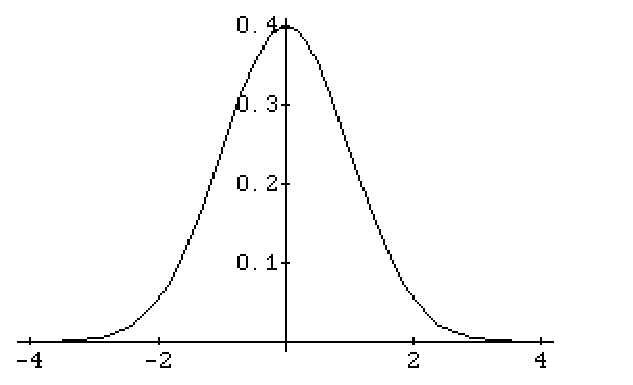
\includegraphics{normal.eps}
%%%%%%%%\end{center}
%%%%%%%%\caption{Curva de Gauss con $\mu=0$ y $\sigma=1$ }
%%%%%%%%\end{figure}



Su función de distribución es, como sabemos :
$$F(x)=\int_{-\infty}^{x} {1\over{\sqrt{2\pi}\sigma}}
{e\vphantom{A}}^{-{1\over 2}{\left({t-\mu}\over{\sigma}\right)}^{2}} dt$$

Que no tiene ninguna expresión algebraica ``decente''. Es por esta razón, y  por comodidad,
que esta función está tabulada.



Cuando una variable tiene distribución normal con parámetros $\mu,\sigma$ la denotamos por
$X\equiv N(\mu,\sigma^2)$


\subsubsection{Resumen v.a con distribución normal, $N(\mu,\sigma^2)$}

\scriptsize
\begin{tabular}{|c|c|c|c|c|}
\hline \begin{tabular}{c} Valores\\ admisibles.\end{tabular} & $f_{X}(x)$ & $F_X(x)=P(X\leq
X)=$ &
 $E(X)$ & $Var(X)$\\\hline & & & &\\
 $D_X=\RR$ & $=\frac{1}{\sqrt{2\pi}\sigma}
          e^{\frac{-(x-\mu)^2}{2\sigma^{2}}}\mbox{ para todo }x\in \R$ & Tabulada la
          $N(0,1)$ & $\mu$ & $\sigma^2$ \\& & & &\\ \hline
\end{tabular}
\normalsize



\subsubsection{Propiedades de la distribución normal.} La función de densidad de la
distribución normal tiene las siguientes propiedades:
\begin{enumerate}[a)]
\item $f$ es continua
\item $\int_{-\infty}^{+\infty} {1\over{\sqrt{2\pi}\sigma}} {e\vphantom{A}}^{-{1\over
2}{\left({x-\mu}\over{\sigma}\right)}^{2}} dx =1$ ( propiedad de todas las densidades).
\item $f(\mu+x)=f(\mu-x)$ y $F(x+\mu)=1-F(\mu-x)$ para todo $x\in \cal{R}$
\item $\lim\limits_{x\to+\infty}f(x)=\lim\limits_{x\to-\infty}f(x)=0$
es decir tiene asíntota horizontal a derecha e izquierda.
\item $f$ es estrictamente creciente si $x<\mu$ y decreciente si $x>\mu$.
\item Alcanza el máximo en $x=\mu$ y en este punto vale $f(\mu)=\frac{1}{\sqrt{2\pi}\sigma}$
\item Tiene dos puntos de inflexión en $x=\mu+\sigma$ y en $x=\mu-\sigma$.
\end{enumerate}


\subsubsection{Transformaciones lineales de variables aleatorias normales}

\begin{proposition} Sea $X\equiv N(\mu,\sigma^2)$  entonces la variable $Y=a X+b$ con
$a\not=0,b\in\cal{R}$ tiene distribución $N(a\mu+b, a^2 \sigma^2)$

En particular si  $X\equiv N(\mu,\sigma^2)$, tomando $a=\frac{1}{\sigma}$ y $b=
\frac{-\mu}{\sigma}$ la v.a. $Z={{X-\mu}\over {\sigma}}$ se distribuye $N(0,1)$.

Esta propiedad es muy importante, ya que utilizándola sólo necesitaremos tabular la
$N(0,1)$. A la función de distribución de una $Z\equiv N(0,1)$ la llamaremos $F_Z$  y a una
normal $N(0,1)$  se le denomina normal estándar. Por lo tanto si
$F_X(x)=F_Z(\frac{x-\mu}{\sigma})$.
\end{proposition}

La propiedad siguiente se desprende de las propiedades generales de una normal y nos será
muy útil en los cálculos de probabilidades de una normal.

\textbf{Propiedad} Si $Z\equiv N((0,1)$ entonces $F_{Z}(x)=1-F_{Z}(-x)$.

\begin{example} Sea $Z\equiv N(0,1)$  Calcular :
\begin{enumerate}[a)]
\item Dado $\delta>0$, $P(-\delta\leq Z \leq
\delta)=F_{Z}(\delta)-F_{Z}(-\delta)=F_Z(3)-(1-F_Z(\delta))=2 F_Z(\delta)-1$
\item $P(-4\leq Z \leq 4)=F_{Z}(4)-F_{Z}(-4)=2 F_Z(4)-1$
\item $P(-2\leq Z \leq 2)=F_{Z}(2)-F_{Z}(-2)=2 F_Z(2)-1$
\item $P(Z\leq -2)=F_Z(-2)=1-F_Z(2)$
\item $P( Z \leq 2)=F_{Z}(2)$
\item $P( Z \geq 2)=1-P(Z<2)=1-F_{Z}(2)$
\item $P( Z > 2)=1-P(Z\leq 2)=1-F_{Z}(2)$
\item $P( Z = 2)=0$
\item $P( Z \geq -2)=1-P(Z< -2)=1-F_{Z}(-2)=1-(1-F_Z(2))=F_Z(2).$
\end{enumerate}
\end{example}
    Resumiendo podemos utilizar las siguientes propiedades, $X\equiv N(\mu,\sigma)$
    \begin{itemize}
    \item  $Z$ es su variable tipificada, es decir,
    $Z=\frac{X-\mu}{\sigma}\equiv N(0,1)$ entonces:

    $$P(X\leq x)=P(\frac{X-\mu}{\sigma}\leq
    \frac{x-\mu}{\sigma})=F_{Z}(\frac{x-\mu}{\sigma})$$

   \item  Cuando tengamos un intervalo
    $$P(a<X<b)=P(\frac{a-\mu}{\sigma}<\frac{X-\mu}{\sigma}<\frac{b-\mu}{\sigma})=$$

    $$=P(\frac{a-\mu}{\sigma}<Z<\frac{b-\mu}{\sigma})=F_{Z}(\frac{b-\mu}{\sigma})-
    F_{Z}(\frac{a-\mu}{\sigma})$$
    \item Si $\delta>0$ $P(\mu-\delta\leq X \leq
\mu+\delta)=2 F_Z(\frac{\delta}{\sigma})-1$
\end{itemize}


    \begin{example}Sea $X$ una normal com media $2$ y varianza $4$, entonces
    \begin{enumerate}[a)]
\item  $P(1< X< 2)= P(\frac{1-2}{2}<\frac{X-2}{2}<\frac{2-2}{2})=
    P(\frac{-1}{2}<Z<0)=F_{Z}(0)-F_{Z}(-0.5)=\frac{1}{2}-1+F_{Z}(0.5).$
    \item $P(X>3)=P(\frac{X-2}{2}>\frac{3-2}{2})=
    P(Z>0.5)=1-F_{Z}(0.5).$
    \end{enumerate}
\end{example}

%%\include{cap5vavect2008}
%%\include{cap6muestreo2008}
%%\include{cap7inferencia}
%%\include{cap8contrateshipotesis}


\chapter{Estadística descriptiva}

Con estas nota de clase iniciamos el curso. El objetivo de este primer capítulo es dar unas
nociones básicas de descripción de datos. Tiene que quedar claro que hay muchas otras
técnicas básicas y avanzadas de descripción de datos que no veremos. Para la resolución
de problemas se tienen que utilizar tanto  la resolución tradicional con papel, lápiz y
calculadora, como la resolución con hojas de cálculo (Excel,OpenOffice\ldots)
o paquetes estadísticos (SPSS, R,\ldots), o programas de propósito todavía más general ( Mathematica, Octave\ldots).
Algunos de estos paquetes están disponibles en los ordenadores de las  aulas de informática de la
universidad y de estos algunos otros tienen licencias que os permiten bajarlos por  internet de forma gratuita; como el OpenOffice (\url{www.openoffice.org})o el paquete
estadístico R (\url{http://www.r-project.org}) en versiones para cualquier sistema operativo usual.




\section{Conceptos básicos}

La estadística es aquella ciencia que tiene por objeto dar métodos tanto para la
 recopilación, organización y análisis de datos
 que provienen de un grupo de individuos, así como  para la decisión de
aceptar o rechazar ciertas afirmaciones o leyes.

Conceptos básicos:
\begin{itemize}
\item Población: Conjunto de todos los individuos que tienen en común alguna
característica observable y de los que se desea estudiar un determinado fenómeno. Sus
 características se definen como  parámetros.

Tipos de población: finita o infinita.
\item Muestra: Es un subconjunto de la población del que se espera
represente a la  población y
 en el que se efectúa el estudio del fenómeno. Sus
características se definen como  estadísticos.
\end{itemize}
\subsection{Estadística descriptiva}

La Estadística Descriptiva se define como aquella ciencia dedicada a describir las
regularidades o características de un conjunto de datos (muestra).

Tareas de la Estadística Descriptiva:
\begin{itemize}
\item Organización de los datos
numéricos de la muestra mediante tablas y  representaciones gráficas.
\item Análisis de los datos obtenidos mediante
la obtención de índices representativos de la muestra como son las medidas de tendencia
central y  de dispersión.
\end{itemize}

\subsection{Estadística Inferencial}

La Estadística Descriptiva basa su estudio sobre las muestras. Ver si éstas son
representativas de la población es  tarea de la estadística inferencial.

La misión principal de la Estadística Inferencial es extraer conclusiones de las
características de la población mediante una muestra representativa de la misma.


\section{Estadística descriptiva}

\subsection{Datos y series estadísticas}

El análisis estadístico parte siempre de un conjunto de datos. Dado un conjunto de
objetos cualesquiera (individuos, países, municipios, etc...), la observación de una
determinada característica o medida de ésta  (cualidad o atributo)  da lugar a un dato
estadístico.

Ejemplos:
\begin{itemize}
\item Población: Países del mundo.

Característica a estudiar: Producto Interior Bruto (P.I.B.). Los datos estadísticos serán
los valores del P.I.B. de los países en cuestión.
\item Población: Estudiantes de segundo curso de Informática.

Característica a estudiar: Altura. Los datos estadísticos serán los valores de la altura
en cm. para cada estudiante.
\end{itemize}

\subsection{Clasificación de los datos}

Una clasificación elemental de los datos estadísticos es la siguiente, dividida en tres
criterios:
\begin{itemize}
\item Tipo de dato
\begin{itemize}
\item Cualitativos o de atributos:  cuando la  comparación entre ellos sólo puede ser de igualdad o
desigualdad.

Por ejemplo: color de los ojos, afiliación política, lugar de residencia, etc,...
\item Ordinales: cuando los datos no son numéricos y la
comparación entre ellos establece un orden.

Por ejemplo: estado de ánimo (valores posibles: depresivo, normal y eufórico), estudios
(valores posibles: ninguno, primarios, secundarios, superiores), etc...
\item Cuantitativas: cuando los datos son
numéricos. Entre los datos cuantitativos podemos señalar dos tipos más:
\begin{itemize}
\item Discretos:  cuando entre dos posibles valores no hay otro.
Por ejemplo: número de  hijos de una familia, número de letras de una palabra en un
texto, etc,...
\item Continuas:  cuando  entre dos posibles valores, siempre podemos encontrar otro valor
posible. Por ejemplo: altura, intereses de una cuenta bancaria, etc,...
\end{itemize}
\end{itemize}
\item Dimensión
\begin{itemize}
\item Unidimensionales: si sólo se considera una única
característica.

Ejemplos: altura, edad, etc,...
\item Multidimensionales: si se consideran conjuntamente varias
características.

Ejemplos: edad y altura, altura y peso, edad, altura y sexo, etc,...
\end{itemize}
\item Tiempo
\begin{itemize}
\item Atemporales:
cuando los datos no están referidos, o no se considera, el momento de tiempo en el que
fueron obtenidos.

Ejemplos: color de los ojos de cierto conjunto de individuos, peso de los  estudiantes que han asistido a 
la clase  de hoy, etc,...
\item Temporales o series cronológicas: en caso contrario.

Ejemplos: P.I.B. anual de Espa\~{n}a durante el periodo 1980 hasta 2004, número de turistas
llegados al aeropuerto de  Palma el mes de agosto durante los a\~{n}os 1970 al 2004, etc,...
\end{itemize}
\end{itemize}

\subsection{Descripción de una serie}

Una vez realizada la recogida de datos, se ha de hacer una representación numérica y
descriptiva de éstos que se adecue de la mejor manera posible al estudio que se desea
realizar.

Cuando los datos son atemporales  y  unidimensionales, es habitual presentarlos en forma
de distribución de frecuencias asociando a cada modalidad o valor las veces que se repite
(frecuencias absolutas).

 En el caso en que los datos sean
bidimensionales y atemporales se suele hacer una tabla de frecuencias de denominada
también como tabla de contingencia.

En el caso en que los datos sean series cronológicas, se representan como una función
matemática en el tiempo, es a decir, una serie de valores $(t, Y_t)$ donde el primer
elemento es el tiempo y  el segundo valor es el dato en ese tiempo.

\subsection{Representación gráfica}

Una vez descrita la serie estadística en forma de tabla, el paso siguiente es
 hacer una representación gráfica de la misma porque lo interesante es observar de golpe
 el aspecto general de los datos.

Veamos con unos cuantos ejemplos en los que  esquemáticamente veremos las
representaciones gráficas más habituales.
\begin{itemize}
\item Diagramas
 de barras. Como ejemplo,  ver en la figura~\ref{ALUMNESTURISME} la representación gráfica
 de la cantidad de alumnos que hay en distintos cursos de informática.

\begin{figure}
\begin{center}
{\tt    \setlength{\unitlength}{0.65pt}
\begin{picture}(161,242)
\thinlines    \put(108,13){\footnotesize TERCERO}
              \put(63,13){\footnotesize SEGUNDO}
              \put(10,13){\footnotesize PRIMERO}
              \put(115,115){125}
              \put(69,88){102}
              \put(22,130){235}
              \put(102,31){\framebox(49,158){}}
              \put(59,31){\framebox(42,118){}}
              \put(10,31){\framebox(49,201){}}
\end{picture}}
\end{center}
\caption {Alumnos de los distintos cursos de Informática} \label{ALUMNESTURISME}
\end{figure}
\item Gráficos de sectores:
Es un gráfico circular dividido en sectores donde cada sector representa el tanto por
ciento de individuos que pertenecen a una determinada modalidad.

\item Pictogramas:
Son representaciones gráficas que guardan relación con el objeto de estudio estadístico.
\end{itemize}

\subsubsection{Diagramas causa-efecto}

Se utilizan en las empresas e industrias, para representar los factores que influyen en un
fenómeno.

Por ejemplo, consideremos el diagrama de la figura \ref{CausaEfecte}:

\begin{figure}
\begin{center}
{\tt\setlength{\unitlength}{0.65pt}
\begin{picture}(213,135)
\thinlines    \put(143,12){TU}
              \put(82,13){TE}
              \put(125,115){ME}
              \put(31,91){MP}
              \put(170,30){\vector(0,1){28}}
              \put(139,46){\vector(1,0){19}}
              \put(121,31){\vector(0,1){30}}
              \put(93,49){\vector(1,0){18}}
              \put(154,102){\vector(0,-1){30}}
              \put(145,108){\vector(0,-1){26}}
              \put(106,95){\vector(1,0){26}}
              \put(63,117){\vector(0,-1){26}}
              \put(37,82){\vector(1,0){36}}
              \put(144,32){\vector(1,1){34}}
              \put(96,34){\vector(1,1){31}}
              \put(115,112){\vector(1,-1){43}}
              \put(47,108){\vector(1,-1){41}}
              \put(10,67){\vector(1,0){193}}
\end{picture}}
\end{center}
\caption{Diagrama causa-efecto} \label{CausaEfecte}
\end{figure}
En la figura anterior tenemos un problema en el que inciden las materias primas
 (MP, 2 diferentes), los métodos de elaboración  (ME, 3 diferentes), la temperatura (TE, 15 grados
 a 20, o bien  de 20 a 30)
y los turnos de trabajo (TU, 2 diferentes).



\section{Variables unidimensionales}

\subsection{Descripción numérica}

La representación ordenada de las observaciones de una muestra se hace mediante una tabla
numérica, en la  que aparecen los valores de la variable y sus frecuencias absolutas;
número de veces que aparece cada dato en la muestra. Además la tabla se puede completar con
las frecuencias absolutas acumuladas.

Mas concretamente, sean  $x_1,\ldots,x_n$ las observaciones de una
 muestra, de tama\~{n}o $n$. Supongamos
que los distintos valores que aparecen en las muestra son $X_1,\ldots,X_J$ y que, si es
posible están ordenados de menor a mayor:
$$X_1<X_2,<\ldots,X_J.$$

Denotaremos por  $n_1$ las veces que aparece el valor $X_1$ en la muestra, $n_2$ las
veces que aparece el valor  $X_2$, $\ldots$, y $n_J$ las veces que aparece el valor
$X_J$. Las frecuencias absolutas serán, por lo tanto los valores:  $n_j,\ j=1,\ldots,J$.

 Es evidente que se verifica la siguiente relación:
$$n=\sum_{j=1}^J n_j$$

Las frecuencias relativas se definen como el cociente entre las absolutas y el  tama\~{n}o de
la muestra: $f_j =\frac{n_j}{ N}$. La frecuencia relativa de $X_j$ es el tanto por uno de
veces que aparece en la muestra. En ocasiones se utilizan los tantos por cien, por
mil,\ldots, pero en la práctica para el cálculo es más cómodo utilizar tantos por uno.

Cuando los datos pueden ser ordenados, se define la frecuencia absoluta acumulada
 $N_j$ del valor $X_j$ como el número de observaciones que son menores o iguales a $X_j$.
 Se verifica la siguiente relación:
$$N_j =\sum_{k=1 }^{j} n_k.$$

La frecuencia relativa acumulada $F_j$ del valor $X_j$ es  el cociente
 entre $N_j$ y $n$, que corresponde a la  suma de las
frecuencias relativas de los datos anteriores a $X_j$. Así podemos escribir
$$F_j =\sum_{k=}^j f_k=\frac{N_j}{ N}.$$

Todos los resultados anteriores se pueden presentar en forma de  tabla, como por ejemplo
la que sigue:
$$
\begin{tabular}{|c|c|c|c|c|}
\hline $X_j$ & $n_j$ & $N_j$ & $f_j$ & $F_j$ \\ \hline \hline $X_1$ & $n_1$ & $N_1$ &
$f_1$ & $F_1$ \\ \hline $X_2$ & $n_2$ & $N_2$ & $f_2$ & $F_2$ \\ \hline $\vdots$ &
$\vdots$ & $\vdots$ & $\vdots$ & $\vdots$ \\ \hline $X_J$ & $n_J$ & $N_J$=n & $f_J$ &
$F_J=1$
\\ \hline \hline Suma $\sum$ & n & & 1 & \\ \hline
\end{tabular}
$$



Cuando los datos son continuos y de una precisión elevada (por ejemplo el tiempo en
segundos, con una precisión hasta milisegundos, de una transmisión) o discretos con un
número elevado de posibles valores (por ejemplo tama\~{n}o en bits de ficheros en un HD), se
corre el riesgo de que las frecuencias resuman escasamente la muestra, es decir que las
frecuencias absolutas de cada valor sean $1$ o  a lo más $2$. En ambos casos se suele
recurrir al conteo de datos por grupos o intervalos de valores a los que se denomina
clases; es lo que se llama recuento de datos agrupados.


Consideremos el caso del peso en kilogramos de una persona. Cuando decimos yo peso 60
kilos ?`qué estoy diciendo en realidad? o si consideramos la edad y digo que tengo 21 a\~{n}os
?`qué estoy diciendo en realidad?

En la variable continua peso en kilos tenemos que los
valores se calculan hasta las unidades, si estamos haciendo una medida en forma correcta
decir que pesamos 60 Kg. debería ser equivalente a decir que pesamos $60\pm 0.5$ Kg, es
decir nuestro instrumento de medida debería medir así; pues el error cometido será la
mitad de la precisión del instrumento de medida. Lo mismo sucede con la edad; cometemos
menos error si decimos que tenemos 21 a\~{n}os cuando tengamos $21\pm 0.5$ a\~{n}os \footnote{
Es evidente que las personas no hacemos esto y que decimos que tenemos 21 a\~{n}os hasta el
día anterior a nuestro aniversario, con lo cual durante la mitad del a\~{n}o, de cada a{\~{n}}o
de nuestra vida, estamos cometiendo un error superior a medio a\~{n}o.}. Así que $60$ Kg.
corresponde al intervalo $(59.5,60.5)$ este tipo de extremos recibe el nombre de límites
reales y puede abarcar más de un tipo de dato, por ejemplo el intervalo $(59,5,70,5)$. Por
contra tenemos los a veces llamados límites aparentes así podríamos definir el
agrupamiento de $60$ a $70$ Kg.

De forma más  general tenemos que si las observaciones vienen dadas con una precisión de
una cifra decimal, los extremos reales de los intervalos serán de la forma $\#.\#5$,
donde el símbolo $\#$ simboliza un dígito para la parte decimal y uno o varios para la
entera.

Por ejemplo si nos dan los datos:
$$1.3, 3.6, 4.7, 4.9, 1.2, 0.6,$$
unos posibles intervalos de agrupamiento con límites reales y de amplitud $1$ son:

$$
\begin{tabular}{c}
$[0.55,1.55)$, \\ $[1.55,2.55)$, \\ $[2.55,3.55)$, \\ $[3.55,4.55)$, \\ $[4.55,5.55)$.
\end{tabular}
$$

Si los valores vienen dados con dos cifras decimales de precisión, los extremos de los
intervalos serían de la forma $\#.\#\# 5.$. Por ejemplo, si los datos son:
$$
0.23, 1.26, 3.54, 5.76, 8.76, 3.67,$$ unos posibles intervalos con límites reales de
amplitud 2 son:
$$
\begin{tabular}{c}
$[0.225,2.225)$, \\ $[2.225,4.225)$, \\ $[4.225,6.225)$, \\ $[6.225,8.225)$, \\
$[8.225,10.225)$.
\end{tabular}
$$

Para escoger el primer extremo se suele calcular el mínimo de la muestra y se toma  como
valor mínimo el extremo  inferior del límite real de ese valor.

En el primer ejemplo, el valor mínimo era $0.6$; por lo tanto el primer extremo es
$0.6-0.05=0.55.$ En el segundo ejemplo, el valor mínimo es $0.23$; por lo tanto, el
primer extremo será $0.23-0.005=0.225$.

Los otros extremos se obtienen sumando una amplitud, de la misma precisión que los datos,
desde el valor mínimo.




Como receta general, que no es de obligado cumplimiento, a la hora de agrupar se
recomienda:


\begin{enumerate}[i)]
\item Decidir el número de clases a considerar. Este número no debe ser inferior a $5$  y
como máximo entre $15$ y $20$. Se pueden utilizar las siguientes heurísticas, si $J$ es
el número de clases tomar $J\geq \sqrt{n}$ (para tama\~{n}os muestrales inferiores a 150)  o
también $2^J\geq n$.
\item Seleccionar los límites de clase que definen los intervalos, de forma que, si es
posible, todos tengan la misma amplitud, salvo quizás los extremos.
\item Intentar no dejar clases con frecuencias muy bajas, para evitar esto se pueden
unir estas clases a una de sus adyacentes.
\end{enumerate}

A cada clase o agrupamiento se le asigna ahora un valor representativo que recibe el
nombre de marca de clase. Se suele tomar, salvo que se diga lo contrario, como marca de
clase el punto medio de un intervalo; que se obtiene dividiendo por dos la amplitud del
mismo.

En el primer ejemplo las marcas de clase son:
$$\begin{tabular}{lr}
\hline $[0.55,1.55)$ & $1.05$ \\ $[1.55,2.55)$ & $2.05$ \\ $[2.55,3.55)$ & $3.05$ \\
$[3.55,4.55)$ & $4.05$ \\ $[4.55,5.55)$ & $5.05$ \\ \hline
\end{tabular}
$$

mientras que para el segundo son estas:
$$\begin{tabular}{lc}
\hline $[0.225,2.225)$ & $1.225$ \\ $[2.225,4.225)$ & $3.225$ \\ $[4.225,6.225)$ &
$5.225$ \\ $[6.225,8.225)$ & $7.225$ \\ $[8.225,10.225)$ & $9.225$ \\ \hline
\end{tabular}
$$


La tabla final es:
$$
\begin{tabular}{lccccc}
intervalos & \begin{tabular}{c}{\footnotesize (Marca de clase)}\\$X_j$ \end{tabular}  &
$n_j$ & $N_j$ & $f_j$ & $F_j$
\\ \hline \hline $[L_1,L_2)$ & $X_1$ & $n_1$ & $N_1$ & $f_1$ & $F_1$ \\ \hline
$[L_2,L_3)$ & $X_2$ & $n_2$ & $N_2$ & $f_2$ & $F_2$ \\ \hline $\vdots$ & $\vdots$ &
$\vdots$ & $\vdots$ & $\vdots$ & $\vdots$ \\ \hline $[L_J,L_{J+1})$ & $X_I$ & $n_I$ &
$N_I$ & $f_I$ & $F_I$
\\ \hline \hline Suma $\sum$ & & n & & 1 & \\ \hline
\end{tabular}
$$

\begin{example}
\label{especial} Consideremos las puntuaciones de $50$ aspirantes a un puesto de trabajo:
{\rm
$$\begin{tabular}{cccccccccc}
8 & 11 & 11 & 8 & 9 & 10 & 16 & 6 & 12 & 19 \\ 13 & 6 & 9 & 13 & 15 & 9 & 12 & 16 & 8 & 7
\\ 14 & 11 & 15 & 6 & 14 & 14 & 17 & 11 & 6 & 9 \\ 10 & 19 & 12 & 11 & 12 &  6 & 15 & 16
& 16 & 12 \\ 13 & 12 & 12 & 8 & 17 & 13 & 7 & 12 & 14 & 12
\end{tabular}
$$
}

La tabla de frecuencias agrupadas con límites reales y amplitud fija de los intervalos
$3$ es:

$$
\begin{tabular}{lccccc}
intervalos  & $X_j$ & $n_j$ & $N_j$ &  $f_j$ &  $F_j$ \\ \hline $[5.5,8.5)$  & \ 7  & 11
& 11 & 0.22 &  0.22 \\ $[8.5,11.5)$ & 10  & 11  & 22  & 0.22  & 0.44 \\ $[11.5,14.5)$ &
13 & 17  & 39  & 0.34  & 0.78 \\ $[14.5,17.5)$ & 16 & \ 9  & 48 & 0.18  & 0.96 \\
$[17.5,20.5)$ & 19   & \ 2  & 50 & 0.04  & 1.00 \\ \hline
\end{tabular}
$$
\end{example}

\subsection{Descripción gráfica}

La representación gráfica de  los datos cuantitativos discretos se hace mediante
diagramas de barras.

 El gráfico~\ref{FAAVQD}  nos muestra el diagrama de barras de las frecuencias absolutas y
 absolutas acumuladas para  variables
discretas. Las frecuencias absolutas $n_i$ son las alturas de las barras con base el
punto~$X_i$. Las frecuencias absolutas acumuladas~$N_i$ son también las alturas de las
barras con base el punto $X_i$.


\begin{figure}
$$
\begin{tabular}{ll}
{\tt    \setlength{\unitlength}{0.70pt}
\begin{picture}(255,178)
\thinlines    \put(210,143){$n_I$}
              \put(128,102){$n_2$}
              \put(76,160){$n_1$}
              \put(200,14){$X_I$}
              \put(141,13){$\cdots$}
              \put(111,14){$X_2$}
              \put(61,14){$X_1$}
              %\put(210,136){\line(-3,-4){38}}
              \put(210,31){\line(0,1){104}}
              %\put(72,153){\line(1,-1){56}}
              \put(127,31){\line(0,1){67}}
              %\put(72,154){\line(-1,-4){31}}
              \put(72,31){\line(0,1){123}}
              \put(10,31){\line(1,0){229}}
              \put(29,167){\line(0,-1){154}}
\end{picture}}
& {\tt    \setlength{\unitlength}{0.70pt}
\begin{picture}(249,228)
\thinlines    \put(31,11){\line(0,1){207}}
              \put(193,193){$N_I$}
              \put(118,153){$N_2$}
              \put(72,88){$N_1$}
              \put(160,170){$\cdots$}
              \put(196,184){\line(1,0){28}}
              \put(196,31){\line(0,1){153}}
              \put(121,144){\line(1,0){42}}
              \put(121,77){\line(0,1){67}}
              \put(78,31){\framebox(43,45){}}
              \put(196,14){$X_I$}
              \put(160,14){$\cdots$}
              \put(118,14){$X_2$}
              \put(72,14){$X_1$}
              \put(10,31){\line(1,0){229}}
\end{picture}}
\end{tabular}
$$
\caption{Frecuencias absolutas. Variables discretas} \label{FAAVQD}
\end{figure}


La descripción gráfica  de los datos continuos (agrupados) se hace mediante histogramas.
En la figura~\ref{FAAVQC} tenemos un ejemplo de histograma. En este caso es el histograma
de  las frecuencias absolutas a la izquierda y a la derecha tenemos el gráfico de las
frecuencias absolutas acumuladas. Las frecuencias absolutas $n_j$ del gráfico de la
izquierda representen las areas de los rectángulos de la base $L_{j+1}-L_j$ (amplitud del
intervalo de clase) mientras que las frecuencias absolutas acumuladas $N_j$ del gráfico
de la derecha representen las alturas de los rectángulos de base $L_{i+1}-L_i$. La curva
 que une los pares ordenados $(X_j,h_j)$ recibe el nombre
  se llama  polígono de frecuencias absolutas (léase igual para relativas), mientras que el polígono
  de frecuencias absolutas acumuladas (de forma similar para relativas) es el formado por los puntos
  $(L_1,0),(L_2,N_1),\ldots,(L_{J+1},N_J)$.

\begin{figure}
%%%\begin{tabular}{ll}
%%%\beginpicture
%%%\setcoordinatesystem units < 0.5cm, 0.5cm> \setlinear
%%%%
%%%% Fig POLYLINE object
%%%%
%%%\linethickness= 0.500pt \setplotsymbol ({\thinlinefont .}) \putrule from  2.508 22.892 to
%%%2.508 12.732
%%%%
%%%% Fig POLYLINE object
%%%%
%%%\linethickness= 0.500pt \setplotsymbol ({\thinlinefont .}) \putrule from  2.032 13.208 to
%%%14.256 13.208
%%%%
%%%% Fig POLYLINE object
%%%%
%%%\linethickness= 0.500pt \setplotsymbol ({\thinlinefont .}) \putrectangle corners at 5.842
%%%15.431 and  7.906 13.208
%%%%
%%%% Fig POLYLINE object
%%%%
%%%\linethickness= 0.500pt \setplotsymbol ({\thinlinefont .}) \putrectangle corners at 3.778
%%%18.447 and  5.842 13.208
%%%%
%%%% Fig POLYLINE object
%%%%
%%%\linethickness= 0.500pt \setplotsymbol ({\thinlinefont .}) \putrectangle corners at
%%%10.763 17.494 and 12.827 13.208
%%%%
%%%% Fig POLYLINE object
%%%%
%%%\linethickness= 0.500pt \setplotsymbol ({\thinlinefont .}) \plot  2.985 13.208  4.731
%%%18.447 /
%%%%
%%%% Fig POLYLINE object
%%%%
%%%\linethickness= 0.500pt \setplotsymbol ({\thinlinefont .}) \plot  4.731 18.447  4.731
%%%18.447 /
%%%%
%%%% Fig POLYLINE object
%%%%
%%%\linethickness= 0.500pt \setplotsymbol ({\thinlinefont .}) \plot  4.731 18.447  6.953
%%%15.431 / \putrule from  6.953 15.431 to  6.794 15.431
%%%%
%%%% Fig POLYLINE object
%%%%
%%%\linethickness= 0.500pt \setplotsymbol ({\thinlinefont .}) \plot 11.557 17.494  9.811
%%%15.589 /
%%%%
%%%% Fig POLYLINE object
%%%%
%%%\linethickness= 0.500pt \setplotsymbol ({\thinlinefont .}) \plot 11.557 17.494 11.557
%%%17.494 /
%%%%
%%%% Fig POLYLINE object
%%%%
%%%\linethickness= 0.500pt \setplotsymbol ({\thinlinefont .}) \plot 11.557 17.494 13.462
%%%13.208 /
%%%%
%%%% Fig POLYLINE object
%%%%
%%%\linethickness= 0.500pt \setplotsymbol ({\thinlinefont .}) \setdots < 0.0953cm> \plot
%%%4.731 13.208  4.731 11.779 /
%%%%
%%%% Fig POLYLINE object
%%%%
%%%\linethickness= 0.500pt \setplotsymbol ({\thinlinefont .}) \plot  6.794 13.208  6.794
%%%11.779 /
%%%%
%%%% Fig POLYLINE object
%%%%
%%%\linethickness= 0.500pt \setplotsymbol ({\thinlinefont .}) \plot 11.716 13.208 11.716
%%%11.779 /
%%%%
%%%% Fig TEXT object
%%%%
%%%\put {$L_1$} [lB] at  3.778 12.414
%%%%
%%%% Fig TEXT object
%%%%
%%%\put {$L_2$} [lB] at  5.842  12.414
%%%%
%%%% Fig TEXT object
%%%%
%%%\put {$L_3$} [lB] at  7.906 12.414
%%%%
%%%% Fig TEXT object
%%%%
%%%\put {$L_I$} [lB] at 10.763 12.414
%%%%
%%%% Fig TEXT object
%%%%
%%%\put {$L_{I+1}$} [lB] at 12.827 12.414
%%%%
%%%% Fig TEXT object
%%%%
%%%\put {$X_1$} [lB] at  4.81 11.144
%%%%
%%%% Fig TEXT object
%%%%
%%%\put {$X_2$} [lB] at  6.837 11.144
%%%%
%%%% Fig TEXT object
%%%%
%%%\put {$X_J$} [lB] at 11.794 11.144
%%%%
%%%% Fig TEXT object
%%%%
%%%\put {$n_1$} [lB] at  4.413 18.923
%%%%
%%%% Fig TEXT object
%%%%
%%%\put {$n_2$} [lB] at  6.953 15.907
%%%%
%%%% Fig TEXT object
%%%%
%%%\put {$n_J$} [lB] at 11.398 18.288
%%%%
%%%% Fig TEXT object
%%%%
%%%\put {$\ldots$} [lB] at  8.700 12.414
%%%%
%%%% Fig TEXT object
%%%%
%%%\put {$\ldots$} [lB] at  8.382 14.637 \linethickness=0pt \putrectangle corners at  2.032
%%%22.892 and 14.256 11.144
%%%\endpicture
%%%&
%%%\beginpicture
%%%\setcoordinatesystem units < 0.5cm, 0.5cm> \setshadesymbol ({\thinlinefont .}) \setlinear
%%%%
%%%% Fig POLYLINE object
%%%%
%%%\linethickness= 0.500pt \setplotsymbol ({\thinlinefont .}) \putrule from  2.508 22.892 to
%%%2.508 12.732
%%%%
%%%% Fig POLYLINE object
%%%%
%%%\linethickness= 0.500pt \setplotsymbol ({\thinlinefont .}) \putrule from  2.032 13.208 to
%%%14.256 13.208
%%%%
%%%% Fig POLYLINE object
%%%%
%%%\linethickness= 0.500pt \setplotsymbol ({\thinlinefont .}) \setdots < 0.0953cm> \plot
%%%4.731 13.208  4.731 11.779 /
%%%%
%%%% Fig POLYLINE object
%%%%
%%%\linethickness= 0.500pt \setplotsymbol ({\thinlinefont .}) \plot  6.794 13.208  6.794
%%%11.779 /
%%%%
%%%% Fig POLYLINE object
%%%%
%%%\linethickness= 0.500pt \setplotsymbol ({\thinlinefont .}) \plot 11.716 13.208 11.716
%%%11.779 /
%%%%
%%%% Fig POLYLINE object
%%%%
%%%\linethickness= 0.500pt \setplotsymbol ({\thinlinefont .}) \setsolid \putrectangle
%%%corners at  3.778 15.748 and  5.842 13.208
%%%%
%%%% Fig POLYLINE object
%%%%
%%%\linethickness= 0.500pt \setplotsymbol ({\thinlinefont .}) \putrectangle corners at 5.842
%%%18.447 and  7.906 13.208
%%%%
%%%% Fig POLYLINE object
%%%%
%%%\linethickness= 0.500pt \setplotsymbol ({\thinlinefont .}) \putrectangle corners at
%%%10.604 20.669 and 12.827 13.208
%%%%
%%%% Fig POLYLINE object
%%%%
%%%\linethickness= 0.500pt \setplotsymbol ({\thinlinefont .}) \putrule from  3.778 13.208 to
%%%3.778 13.208 \plot  3.778 13.208  5.842 15.748 / \plot  5.842 15.748  7.906 18.447 /
%%%%
%%%% Fig POLYLINE object
%%%%
%%%\linethickness= 0.500pt \setplotsymbol ({\thinlinefont .}) \plot 12.827 20.669 10.604
%%%20.034 / \plot 10.604 20.034  9.652 19.082 /
%%%%
%%%% Fig TEXT object
%%%%
%%%\put {$L_2$} [lB] at  5.842 12.414
%%%%
%%%% Fig TEXT object
%%%%
%%%\put {$L_1$} [lB] at  3.778 12.414
%%%%
%%%% Fig TEXT object
%%%%
%%%\put {$X_1$} [lB] at  4.81 11.144
%%%%
%%%% Fig TEXT object
%%%%
%%%\put {$X_2$} [lB] at  6.873 11.144
%%%%
%%%% Fig TEXT object
%%%%
%%%\put {$L_3$} [lB] at  7.906 12.414
%%%%
%%%% Fig TEXT object
%%%%
%%%\put {$\ldots$} [lB] at  8.700 12.414
%%%%
%%%% Fig TEXT object
%%%%
%%%\put {$L_J$} [lB] at 10.604 12.414
%%%%
%%%% Fig TEXT object
%%%%
%%%\put {$X_J$} [lB] at 11.794 11.144
%%%%
%%%% Fig TEXT object
%%%%
%%%\put {$L_{J+1}$} [lB] at 12.688 12.414
%%%%
%%%% Fig TEXT object
%%%%
%%%\put {$N_1$} [lB] at  4.096 16.224
%%%%
%%%% Fig TEXT object
%%%%
%%%\put {$N_2$} [lB] at  6.477 18.764
%%%%
%%%% Fig TEXT object
%%%%
%%%\put {$N_J$} [lB] at 11.081 20.987
%%%%
%%%% Fig TEXT object
%%%%
%%%\put {$\ldots$} [lB] at  8.382 19.399 \linethickness=0pt \putrectangle corners at  2.032
%%%22.892 and 14.256 11.144
%%%\endpicture
%%%\end{tabular}
\begin{center}
\includegraphics{frecuencias.eps}
\end{center}
\caption{Frecuencias absolutas. Variables continuas} \label{FAAVQC}
\end{figure}

\begin{example}
Consideremos las puntuaciones de los $50$ aspirantes del ejemplo~\ref{especial}. Tomamos
intervalos  de amplitud $3$. El histograma de frecuencias absolutas con el
correspondientes polígono de frecuencias acumuladas se muestra en la
figura~\ref{EXEMPLE2}.

Notemos que las alturas de los rectángulos se calculan teniendo en cuenta que la amplitud
de los intervalos es~$3$:
\[
\begin{array}{rlcrl}
h_1 =& \frac{n_1}{3}=\frac{11}{3}=3.6666,& & h_2=& \frac{n_2}{3}= \frac{11}{3}=3.666,\\
&&&&\\ h_3 =& \frac{n_3}{3}=\frac{17}{3}=5.6666,& & h_4=& \frac{n_4}{3}= \frac{9}{3}=3,
\\ &&&&\\ h_5 = & \frac{n_5}{3}=\frac{2}{3}=0.666.&&&
\end{array}
\]

\begin{figure}
%%%$$
%%%\setcoordinatesystem units <0.5cm,0.25cm>
%%%\beginpicture
%%%\setplotarea x from 5.5 to 20.5, y from 0 to 20 \axis bottom shiftedto y=0 ticks in
%%%withvalues $5.5$ $8.5$ $11.5$ $14.5$ $17.5$ $20.5$ / quantity 6 / \axis left shiftedto
%%%x=5.5 ticks in withvalues {} $2$ $4$ $6$ / quantity 4 / \sethistograms \plot 5.5 0 8.5 11
%%%11.5 11 14.5 17 17.5 9 20.5 2 / \setlinear \plot 4 0 7 11 10 11 13 17 16 9 19 2 22 0 /
%%%\endpicture
%%%$$
\begin{center}
\includegraphics{histograma.eps}
\end{center}
 \caption {Histograma de frecuencias absolutas (ejemplo 1)} \label{EXEMPLE2}
\end{figure}
\label{PUNTUACIONS}
\end{example}

\section{Análisis de las distribuciones}

El análisis de las distribuciones de una variable o dato estadístico consiste en reducir
los datos estadísticos a unas pocas medidas o índices, que reciben el nombre de
estadísticos, que nos permitan una interpretación de las regularidades de todo el
colectivo.

Tenemos los siguientes tipos de medidas:
\begin{itemize}
\item Medidas de posición:
Intentan representar toda la distribución. Las más importantes son la media aritmética,
la moda y la mediana.
\item Medidas de dispersión: Intentan se\~{n}alar la
dispersión o separación del conjunto de datos respecto a las medidas de posición
 adoptadas. Las más importantes son la varianza,
la desviación típica, el coeficiente de variación  y los recorridos.
\item Medidas de simetría y apuntamiento: Estudian si el  polígono de frecuencias relativas
es simétrico y lo \emph{estirado} que está (apuntamiento). Se suele comparar este
polígono con la curva de frecuencias de una distribución ideal llamada normal o campana
de Gauss.
\item Otras como las medidas de concentración; que no veremos. Por ejemplo el índice de Gini.
\end{itemize}

\textbf{Nota importante:} Algunas de estas medidas sólo se pueden calcular cuando tenga
sentido operar con los datos, es decir, si estos son cantidades o al menos órdenes. Si
tengo que una variable que responde al deporte que practica una persona de determinad
población, aunque la variable esté codificada a valores enteros, no tiene sentido hacer
la media aritmética. En lo que sigue dejaremos al lector que decida, siempre de forma razonada, que estadísticos no son
aplicables a estas variables.

\subsection{Medidas de posición}
Veremos aquí las más conocidas medidas de posición.

\subsubsection{Media aritmética}

 La media aritmética  es la medida de tendencia central más utilizada,
simboliza el valor central de toda la distribución. Su fórmula general es\footnote{Como
se ve damos dos fórmulas una para datos no agrupados y otra para datos posiblemente
agrupados, en lo que sigue no especificaremos  cuales son las fórmulas para datos
agrupados o no.}:

$$overline{x}=\frac{x_1 + x_2 +\ldots +
x_n}{n}=\frac{\sum\limits_{j=1}^{J} n_j X_j}{n}=\sum\limits_{j=1}^{J} f_j X_j.$$


Para el caso de distribuciones de variables discretas, los $X_j$ son los posibles valores de la
variable mientras que  en el caso continuo, son las marcas de clase de los intervalos.

Una de las propiedades fundamentales de la media es que si  hacemos una transformación lineal
de los datos digamos $Y=aX+b$\footnote{Multiplicar por una constante positiva se suel denominar cambio de escala. SUmar una constante a una varible recibe el nombre de cambio de origen. Así podemos decir que la media arimética queda igual de afectada por  los cambios de escala y origen en los datos.} donde $X$ son los valores de la variable, la relación
entre la media aritmética de $Y$ y la de $X$ es:

$$ \overline{y}=a \overline{x} +b.$$

\subsubsection{Medias armónica y geométrica}

Las medias armónica y geométrica no son de gran utilidad salvo en problemas concretos. Se
calculan de la siguiente forma:

\[ M_{h}=\frac{n}{\sum\limits_{i=1}^{n} \frac{1}{x_i}}=\frac{n}{\sum\limits_{j=1}^{I} \frac{n_j}{X_j}}, \quad  M_g
=\root n\of{\prod_{i=1}^{n} x_j} =\root n\of{\prod_{j=1}^{I} X_j^{n_j}}.\]


Estas medias tienen restricciones sobre los datos, no pueden tener datos nulos, y en
general se utilizan para datos positivos.

\begin{example}
Consideremos los siguientes datos: {\rm
$$
\begin{tabular}{cccccccccc}
10 & 5 & 2 & 7 & 9 & 5 & 7 & 6 & 5 & 9 \\ 12 & 2 & 6 & 6 & 9 & 12 & 6 & 6 & 6 & 4 \\
 9 & 7 & 12 & 11 & & & & & &
\end{tabular}
$$
} La media aritmética de los datos anteriores sin agrupar en intervalos es:

$$\overline{x}= \frac{10+5+2+\cdots +12+11}{24}=\frac{173}{24}=7.20833
$$

Si los agrupamos en intervalos de amplitud $3$, la media será (hacemos primero la
correspondiente tabla de frecuencias){\rm
$$
\begin{tabular}{l|ccc|}
intervalos    & $X_j$ & $n_j$ & $n_jX_j$ \\ \hline $[1.5,4.5)$   &  \ 3 &  \ 3 &   \ 9 \\
\hline $[4.5,7.5)$   &  \ 6  & 12 &  72 \\ \hline $[7.5,10.5)$  &  \ 9 &  \ 5 &  45 \\
\hline $[10.5,13.5)$ & 12  &  \ 4 &  48 \\ \hline
  Suma        &   & 24   & 174
\end{tabular}
$$
 }
$$\overline{x}= \frac{174}{24}=7.25$$
Notemos que los valores difieren ya que el agrupamiento provoca una pérdida de
información.
\end{example}

\subsubsection{Media general de orden m}

Definimos la media general $M_{(m)}$ de orden $m$ como:

$$M_{(m) }=\left(\frac{\sum_{i=1}^n  n_i x_i^m}{n}\right)^{\frac{1}{m}}=
\left(\frac{\sum_{j=1}^J  n_j X_j^m}{n}\right)^{\frac{1}{m}}$$

Se cumple que:

$$M_{(-1)}=M_h;\,  M_{(0)}=M_g;\,  M_{(1)}=\overline{x}$$


Además se cumple que $M_{(m)}$ es una función creciente en $m$ y por lo tanto :

$$M_h\leq M_g\leq \overline{x}.$$


\subsubsection{Mediana y percentiles}

La mediana es aquel valor que, cuando consideremos todos los valores de la muestra
ordenados, ocupa el  lugar central. Es decir, quedan la misma cantidad de valores a su
izquierda que a su derecha.

Supongamos que los datos ordenados son $x_1, x_2,\ldots x_n$, la\textbf{ mediana} vale:

\begin{eqnarray*}
x_{\frac{n+1}{2}}, &\mbox{ si } \mbox{$n$  es impar,}\\
\frac{x_{\frac{n}{2}}+x_{\frac{n}{2}+1}}{2},&\mbox{ si }\mbox{$n$ es par.}
\end{eqnarray*}

Por ejemplo, la mediana de los datos $1,2,5,8,8,9,11$ vale $8$ ya que $8$ es el que ocupa
el lugar central y la mediana de $2,3,3,4,5,6$ vale $\frac{3+4}{2}=3.5$.

La manera anterior de calcular la mediana no es práctica en el caso en que haya muchos
datos es muy costoso ordenarlos ( orden $n^2$ o $n\log(n)$). Veamos alguna manera de
cálculo aproximado de la mediana a partir de la tabla de distribución de frecuencias.

Necesitaremos las columnas de frecuencias absolutas y la de frecuencias absolutas
acumuladas:

$$
\begin{tabular}{l|ccc|}
intervalos & $X_j$ & $n_j$ &$ N_j$ \\ \hline \hline $[L_1, L_2)$ & $X_1$ & $n_1$ & $N_1$
\\ $[L_2, L_3)$ & $X_2$ & $n_2$ & $N_2$ \\ \hline $\vdots$ & $\vdots$ & $\vdots$ &
$\vdots$ \\ \hline $[L_I, L_{I+1})$ & $X_I$ & $n_I$ & $N_I$ \\ \hline $\sum$ & & $n$ &
\end{tabular}
$$

Llamaremos intervalo crítico para la mediana al primer intervalo en el que su frecuencia
absoluta acumulada supere o iguale a $\frac{n}{2}$. Denotemos por $[L_c, L_{c+1})$  el
intervalo crítico. Sea $N_{c-1}$ la frecuencia absoluta acumulada del intervalo anterior
al crítico. En el caso en que el interval crítico sea  el primero, $N_{c-1}=0$. Sea $n_c$
la  frecuencia absoluta del intervalo crítico. Sea  $A_c=L_{c+1}-L_c$ la amplitud del
intervalo crítico. Calcularemos la \textbf{mediana} mediante:

$$M=L_{c}+A \frac{\left(\frac{n}{2}- N_{c-1}\right)}{n_c}.$$

La justificación de la fórmula anterior es la siguiente: si representásemos las
frecuencias absolutas acumuladas entre los extremos de los intervalos, la mediana seria
la antiimagen de $\frac{n}{2}$ en  el intervalo crítico haciendo una interpolación por
rectas (ver figura~\ref{MEDIANA}).

\begin{figure}
%%%$$
%%%\beginpicture
%%%\setcoordinatesystem units < 0.75cm, 0.75cm> \setshadesymbol ({\thinlinefont .})
%%%\setlinear
%%%%
%%%% Fig POLYLINE object
%%%%
%%%\linethickness= 0.500pt \setplotsymbol ({\thinlinefont .}) \putrule from  2.508 22.415 to
%%%2.508 14.954
%%%%
%%%% Fig POLYLINE object
%%%%
%%%\linethickness= 0.500pt \setplotsymbol ({\thinlinefont .}) \putrule from  1.873 15.589 to
%%%10.287 15.589 \putrule from 10.287 15.589 to 10.128 15.589
%%%%
%%%% Fig POLYLINE object
%%%%
%%%\linethickness= 0.500pt \setplotsymbol ({\thinlinefont .}) \setdots < 0.0953cm> \plot
%%%4.096 15.589  4.096 17.177 /
%%%%
%%%% Fig POLYLINE object
%%%%
%%%\linethickness= 0.500pt \setplotsymbol ({\thinlinefont .}) \plot  6.636 15.589  6.636
%%%19.399 /
%%%%
%%%% Fig POLYLINE object
%%%%
%%%\linethickness= 0.500pt \setplotsymbol ({\thinlinefont .}) \plot  8.064 20.510  8.064
%%%15.589 /
%%%%
%%%% Fig POLYLINE object
%%%%
%%%\linethickness= 0.500pt \setplotsymbol ({\thinlinefont .}) \setsolid \plot  4.096 17.177
%%%8.223 20.669 /
%%%%
%%%% Fig POLYLINE object
%%%%
%%%\linethickness= 0.500pt \setplotsymbol ({\thinlinefont .}) \setdots < 0.0953cm> \plot
%%%3.937 17.177  2.508 17.177 /
%%%%
%%%% Fig POLYLINE object
%%%%
%%%\linethickness= 0.500pt \setplotsymbol ({\thinlinefont .}) \plot  6.636 19.399  2.508
%%%19.399 /
%%%%
%%%% Fig POLYLINE object
%%%%
%%%\linethickness= 0.500pt \setplotsymbol ({\thinlinefont .}) \plot  8.064 20.510  2.508
%%%20.510 /
%%%%
%%%% Fig TEXT object
%%%%
%%%\put {$L_c$} [lB] at  3.620 14.796
%%%%
%%%% Fig TEXT object
%%%%
%%%\put {$L_{c+1}$} [lB] at  7.747 14.796
%%%%
%%%% Fig TEXT object
%%%%
%%%\put {$M$} [lB] at  6.318 14.796
%%%%
%%%% Fig TEXT object
%%%%
%%%\put {$N_{c-1}$} [lB] at  1.238 17.018
%%%%
%%%% Fig TEXT object
%%%%
%%%\put {${n\over 2}$} [lB] at  1.238 19.241
%%%%
%%%% Fig TEXT object
%%%%
%%%\put {$N_c$} [lB] at  1.238 20.352 \linethickness=0pt \putrectangle corners at  0.286
%%%22.415 and 10.287 14.796
%%%\endpicture
%%%$$
%%%%CAMBIAR DIBUJO N/2 -> n/2 y mejorar
\begin{center}
\includegraphics{interpretacion.eps}
\end{center}
\caption{Interpretación geométrica de la Mediana} \label{MEDIANA}
\end{figure}

Los percentiles son una generalización de la mediana. La mediana es el percentil~50 ya
que deja el 50\% de las observaciones a su izquierda.

En general el \textbf{percentil}~$P$ es aquel valor que deja el~$P\%$ de las
observaciones a su izquierda. El cálculo, dada la distribución de frecuencias es
semejante al cálculo de la mediana.

Definimos el  intervalo crítico  en  este caso  como el primer intervalo del que su
frecuencia absoluta acumulada supera o iguala a $\frac{n\cdot P}{100}$.


Sean entonces, $[L_c, L_{c+1})$ el intervalo crítico,  $N_{c-1}$ la frecuencia absoluta
acumulada del intervalo anterior al crítico y  $n_c$ la
 frecuencia absoluta del intervalo
crítico. Si denomamos por  $A_c$ a la amplitud  del intervalo crítico, la fórmula
 para calcular el  \textbf{percentil}~$P$ es:

$$M_p =L_c + A_c \frac{\left(\frac{n\cdot P}{100}-N_{c-1}\right)}{n_c}.$$

\begin{example}
Calculemos la mediana, sin agrupar,  de los siguientes datos:

$$
14, 15, 16, 18, 18, 18, 18, 19, 20, 20, 22.
$$
El tama\~{n}o de la muestra es $n=11$ observaciones y ya están ordenadas. El lugar central,
es el que ocupa  el sexto puesto, el valor que ocupa este lugar es el $18$, por lo tanto,
la mediana es $18$.

En la siguiente muestra tenemos un número par de datos:
$$
24, 25, 26, 26, 27, 27, 27, 29.
$$
El tama\~{n}o muestral es $n=8$ observaciones que ya están ordenadas. El lugar central estará
entre el  cuarto y el quinto puesto. Los datos que ocupan estos lugares son el $26$ y el
$27$. Por lo tanto la mediana vale

$$M=\frac{26+27}{2}=26.5.$$
\end{example}

\begin{example}
Consideremos la siguiente  distribución de frecuencias: {\rm
$$
\begin{tabular}{lccc}
intervalos &  $X_j$ &  $n_j$ &  $N_j$ \\ \hline $[1.5,4.5)$   & \ 3  &  \ 3 &   \ 3  \\
$[4.5,7.5)$   & \ 6  & 12 &  15  \\ $[7.5,10.5)$  & \ 9  &  \ 5 &  20  \\ $[10.5,13.5)$ &
12 &  \ 4 &  24  \\ \hline
\end{tabular}
$$
} Tenemos  que $n=24$ y que  $\frac{n}{2}=12$. El intervalo crítico es:
 $[4.5,7.5)$
La mediana valdrá entonces:

$$M=4.5+3\frac{(12-3)}{12}=6.75.$$

Percentil $25$: $25\mbox{\%}\Rightarrow  \frac{n\cdot P}{100}= 6$. Intervalo crítico:
 $[4.5,7.5)$.

$$M_{25}=4.5+3\frac{(6-3)}{12}=5.25$$

Percentil $75$: $75\mbox{\%} \Rightarrow  \frac{n\cdot P}{100}= 18$. Intervalo crítico:
 $[7.5,10.5)$.

$$
M_{75}=7.5+3\frac{(18-15)}{5}=9.3
$$
\end{example}

En general se habla de cuantiles para denominar a todos estos estadísticos. Los cuartiles
que dividen a la población en cuartos son llamados cuartiles, así el primer cuartil $Q_1$
deja a su izquierda el 25\% de las observaciones, el segundo cuartil $Q_2$ es la mediana
y el tercer cuartil $Q_3$ deja a su izquierda el $75\%$ de las observaciones. También se
habla de los deciles que son los estadísticos que dividen a la población en décimas
partes.

\subsubsection{Moda}

La moda de una muestra es un valor que tenga la frecuencia absoluta más grande. En
consecuencia la  moda no tiene por qué ser única puede haber más de un valor con
frecuencia absoluta máxima. Si una distribución tiene una sola moda diremos que es
unimodal, si dos bimodal, \ldots La presencia de dos modas puede indicar la existencia de
dos poblaciones diferenciadas en la muestra (por ejemplo el peso según sexo).



En el caso en que tengamos una tabla de distribuciones, para encontrar la moda, hemos de
localizar el intervalo o intervalos con frecuencia absoluta más alta.

Sean $[L_j, L_{j+1})$ los extremos del intervalo con  frecuencia absoluta máxima.

Para calcular la moda podemos utilizar  la siguiente  fórmula, en la que suponemos que
todos los intervalos tienen la misma amplitud $A$ (en caso contrario se utilizan otras
aproximaciones):

$$M_o =L_j + A \frac{n_{j+1}}{(n_{j-1}+n_{j+1})}.$$

Donde:

\begin{itemize}
\item $A$: amplitud de los intervalos
\item $n_{j-1}$: frecuencia absoluta del intervalo anterior al de
frecuencia máxima.
\item $n_{j+1}$: frecuencia absoluta del intervalo posterior al de
frecuencia máxima.
\end{itemize}

\begin{example}
Consideremos la siguiente distribución de frecuencias: {\rm $$
\begin{tabular}{lccc}
intervalos    & $X_j$ & $n_j$ & $N_j$ \\ \hline $[1.5,4.5) $  &  \ 3 & \ 3 &   \ 3  \\
$[4.5,7.5) $  &  \ 6 &  12 &  15  \\ $[7.5,10.5)$  &  \ 9 &   \ 5 &  20
\\ $[10.5,13.5)$ & 12 &   \ 4 &  24  \\ \hline
\end{tabular}
$$}

El intervalo con la frecuencia absoluta mas alta es el $[4.5,7.5)$. Por lo tanto, la moda
vale:

$$M_0=4.5+3\frac{5}{(3+5)}=6.375.$$
\end{example}



\subsection{Medidas de dispersión}

Una vez estudiadas las medidas de posición, vamos a estudiar algunos estadísticos
 que miden lo separadas que están las observaciones entre sí.

Algunas medidas de dispersión respecto a la media aritmética son la varianza, la
desviación típica, la desviación media respecto de la media y el coeficiente  de
variación.

Las medidas de dispersión respecto a la a la mediana es la desviación media respecto de
la mediana.

Otras medidas de dispersión son el recorrido, el rango , el recorrido intercuartílico, el
rango intercuartílico.

%%%Las medidas de simetría y  apuntamiento (curtosis)  comparan el perfil de la distribución
%%%con el perfil de una distribución normal.

%%%Per últim hi ha els índexos de concentració \index{indexos@índexos!de concentracio@de
%%%concentració} desde el punt de vista d'u\-ni\-for\-mi\-tat de la
%%%distribució\index{distribucio@distribució} com és l'índex de Gini\index{index@índex!de
%%%Gini}.

\subsubsection{Varianza y  desviación típica o estándar}

La varianza y la desviación  típica nos indican si los datos  están muy dispersos
respecto de la media aritmética $\overline{x}$.

La fórmula del cálculo de la varianza es:

$$s^{2}=\frac{1}{n} \sum\limits_{j=1}^{J}
n_j(X_j-\overline{x})^2=\frac{1}{n} \sum\limits_{j=1}^{J} n_j X_j^2- \overline{x}^2.$$

o bien para datos sin agrupar

$$s^{2}=\frac{1}{n} \sum\limits_{j=1}^{n}
(x_i-\overline{x})^2=\frac{1}{n} \sum\limits_{j=1}^{n}  x_i^2- \overline{x}^2.$$

La segunda expresión es más útil que la primera de cara al cálculo de la  varianza.

La propiedad fundamental de la varianza  es que  minimiza las desviaciones  al cuadrado
respecto a cualquier punto $X_0$. Es decir:

$$\min_{X_0} \frac{1}{n} \sum\limits_{j=1}^{J}n_j (X_j - X_0)^2=s^2.$$

La desviación típica o estándar es la raíz cuadrada positiva de la varianza:

$$s=\sqrt{\frac{1}{n} \sum\limits_{j=1}^{J} n_j X_j^2-
\overline{x}^2}.$$

Por motivos que veremos en temas posteriores existe otra fórmula para el cálculo de la
varianza de una muestra a la que en ocasiones se le denomina cuasivarianza o también se le
llama varianza muestral  \footnote{Quizá algunos de vosotros descubra aquí el motivo por el que
las calculadoras llevan dos teclas $s_n^2$ o $\sigma_{n}^2$ y $s_{n-1}$ o
$\sigma_{n-1}$.}:

$$\tilde{s}^2 =\frac{n}{n-1} s^2=\frac{1}{n-1}\sum\limits_{j=1}^{n}n_j(X_j-\overline{X})^2.$$

Notemos que la cuasivarianza es una peque\~{n}a corrección de la varianza, en lugar de
dividir por el tama\~{n}o muestral se divide por el tama\~{n}o muestral menos $1$. Para muestras
grandes la corrección puede resultar insignificante pero para muestras peque\~{n}as es
necesaria.

Cuando  la variable $X$ se vea afectada por un cambio lineal: $Y=aX+b$, la varianza de
$Y$ cumple la siguiente relación:

$$s_Y^2 = a^2 s_X^2.$$

De aquí deducimos que la varianza es independiente respecto a  cambios de origen y que
queda afectada por el cuadrado de los cambios de escala.

Para las desviaciones típicas tendremos:
$$s_Y=|a| s_X.$$

\begin{example}
Consideremos la siguiente distribución de frecuencias{\rm
$$
\begin{tabular}{l|r|r|r|}
intervalos    & $X_j$ & $n_j$ & $n_jX_j$ \\ \hline $[9.5,29.5)$   & 19.5 &  38 &   741.0
\\ $[29.5,49.5)$  & 39.5 &  18 &   711.0 \\ $[49.5,69.5)$  & 59.5 &  31 & 1844.5 \\
$[69.5,89.5)$  & 79.5 &  20 &  1590.0   \\ \hline
    Sumas      &      & 107 &  4886.5
\end{tabular}
$$
} Vamos a calcular la varianza

Primero calculamos la media:

$$\overline{x}=\frac{4886.5}{107}=45.6682$$

Para calcular la varianza hemos de a\~{n}adir dos columnas a la tabla anterior: {\rm
$$
\begin{tabular}{crr}
 $X_j$ & $X_j^2$ & $n_jX_j^2$ \\
\hline
 19.5  & 380.25  & 14449.50 \\
 39.5  & 1560.25 &  28084.50 \\
 59.5  & 3540.25 & 109747.75 \\
 79.5  & 6320.25 & 126405.00 \\
\hline Suma   &          & 278686.75
\end{tabular}
$$
} La varianza y la desviación  típica valen:

$$s_X^2=\frac{278686.75}{107}-45.6682^2=518.962$$
$$s_X=\sqrt{518.962}=22.7807$$
\end{example}

\subsubsection{Coeficiente de variación}

El coeficiente de variación  se define como el cociente entre la desviación
 típica  y la media
aritmética, se utiliza para variables en las que la media represente a la magnitud de los
datos (por ejemplo si todos son positivos y la distribución es unimodal) :

$$CV=\frac{s}{\overline{x}}.$$

El coeficiente de variación  es independiente del cambio de escala. Más concretamente, si
hacemos el cambio lineal  de la variable $X$:
 $Y=a X$, con $a>0$,  el coeficiente de
variación  de la variable $Y$ es el mismo que el de la variable $X$:

$$CV_Y=CV_X.$$

El coeficiente de variación será útil para comparar la dispersión de distribuciones
medidas en diferentes escalas.

\begin{example}

Consideremos la siguiente distribución de frecuencias: {\rm
$$
\begin{tabular}{lccc}
intervalos     & $X_j$ & $n_j$ & $n_jX_j$\\ \hline $[9.5,29.5)$  & 19.5 & \ 38  & \ 741.0
\\ $[29.5,49.5)$ & 39.5 & \ 18  & \ 711.0  \\ $[49.5,69.5)$ & 59.5 & \ 31  & 1844.5 \\
$[69.5,89.5)$ & 79.5 & \ 20  & 1590.0   \\ \hline Sumas     &      & 107 & 4886.5
\end{tabular}
$$
}

La media   y la desviación  típica son:
$$\overline{x}=45.6682,\quad s_X=22.7807$$
Por lo tanto el coeficiente de variación es:
$$CV=\frac{s}{\overline{x}}=\frac{22.6807}{45.6682}=0.4988$$
\end{example}

\subsubsection{Desviación media}

La desviación media es un índice de dispersión respecto a la mediana o a la media. Queda
definido por:

$$D_M=\frac{1}{n}\sum\limits_{j=1}^{J}n_j|X_j - M|.$$

donde $M$ es la mediana o la media aritmética.

La propiedad fundamental de la desviación  media respecto a la mediana es que minimiza
las desviaciones en valor absoluto respecto de un punto cualquiera $X_0$. Es decir:

$$\min_{X_0} \frac{1}{n} \sum\limits_{j=1}^{J}n_j|X_j - X_0|=D_M.$$

\subsubsection{Recorrido}

Otra medida de dispersión es el recorrido. Se define como la diferencia entre el valor
máximo y mínimo de los valores observados.

%%%En el caso de distribuciones agrupadasse entenderá como valor mínimo'entendr\`a com a valor
%%%m\`axim l'extrem de la dreta del últim interval \index{interval} i com a valor mínim
%%%l'extrem de l'esquerra del primer interval. Aquesta mesura\index{mesura} és v\`alida tant
%%%per la media, \index{media} com per la moda com per la mediana.

\begin{example}
Consideremos la siguiente distribución de frecuencias: {\rm
$$
\begin{tabular}{lrrr}
intervalos &\multicolumn{1}{c}{$X_j$} & \multicolumn{1}{c}{$n_j$}
&\multicolumn{1}{c}{$n_j X_j$}\\ \hline $[0.5,15.5) $ &  8 & 4  & 32  \\ $[15.5,30.5)$ &
23 & 4 & 92 \\ $[30.5,45.5)$ & 38 & 2 & 76 \\
 \hline
Sumas     &      & 10 & 200
\end{tabular}
$$
} Vamos a calcular la desviación media:


Calculamos la media

$$\overline{x}=\frac{200}{10}=20$$

A\~{n}adimos dos columnas más a la tabla de frecuencias:


$$
\begin{tabular}{ccc}
$X_j$  & $|X_j-\overline{x}|$ &  $n_j|X_j-\overline{x}|$ \\ \hline \ 8     & 12   &   48
\\ 23     & \ 3     &  12  \\ 38     & 18     &  36   \\ \hline Sumas  &       &  96 \\
\end{tabular}
$$
 La desviación es:

$$D_M=\frac{96}{10}=9.6$$
\end{example}

También se utiliza el recorrido intercuartílico que es $Q_3-Q_1$; la diferencia entre el
tercer y primer cuartil. También se pueden calcular recorridos con deciles, percentiles y
cuantiles en general.

\subsection{Perfil de una distribución}

El perfil de una distribución viene determinado por alguno de sus polígonos de
frecuencias. Es mejor utilizar las frecuencias relativas ya que no dependen del tama\~{n}o de
la muestra. La idea es encontrar la curva a donde tiende el polígono de frecuencias
cuando la muestra se hace grande, que en definitiva sería la curva de frecuencias de toda
la población.

\begin{figure}
%%%$$
%%%\begin{tabular}{ll}
%%%\setcoordinatesystem units <.075cm,.075cm>
%%%\beginpicture
%%%\setplotarea x from 0 to 60, y from 0 to 50 \axis bottom shiftedto y=0 ticks in
%%%withvalues {} {} {} {} {} {} {} /
%%% quantity 7 /
%%%\axis left shiftedto x=0 ticks in withvalues {} {} {} {} {}  /
%%% quantity 5 /
%%%%\arrow <8pt> [0.2,0.67] from 25 75 to 75 65
%%%%\put {$S$} at 23 78
%%%%\put {$A$} [rt] at 0 0
%%%%\put {$C$} [t] at 100 0
%%%%\put {$B$} [lb] at 101 100
%%%\setlinear \putrule from 10 0 to 10 40 \putrule from 20 0 to 20 30 \putrule from 30 0 to
%%%30 20 \putrule from 40 0 to 40 50 \putrule from 50 0 to 50 30 \put {$f_j$} at -5 45 \put
%%%{$\overline x$} at  25 -5
%%%\endpicture
%%%& \setcoordinatesystem units <.075cm,.075cm>
%%%\beginpicture
%%%\setplotarea x from 0 to 60, y from 0 to 50 \axis bottom shiftedto y=0 ticks in
%%%withvalues {} {} {} {} {} {} {} /
%%% quantity 7 /
%%%\axis left shiftedto x=0 ticks in withvalues {} {} {} {} {}  /
%%% quantity 5 /
%%%%\arrow <8pt> [0.2,0.67] from 25 75 to 75 65
%%%%\put {$S$} at 23 78
%%%%\put {$A$} [rt] at 0 0
%%%%\put {$C$} [t] at 100 0
%%%%\put {$B$} [lb] at 101 100
%%%\sethistograms \plot 5 0 15 40 25 30 35 20 45 50 55 30 / \put {$f_j$} at -5 45 \put
%%%{$\overline x$} at  25 -5
%%%\endpicture
%%%\end{tabular}
%%%$$
\begin{center}
\includegraphics{diagrama.eps}
\end{center}
\caption{Diagrama de barras e  histograma de las frecuencias relativas }
\label{RELATIVES}
\end{figure}

Una curva continua en forma de campana llamada curva de Gauss \footnote{Es una buena broma pedir a un amigo el cálculo de la primitiva de la curva de Gauss.} puede servir como un modelo
matemático ideal para comparar el perfil de cualquier distribución. Esta curva
corresponde a la gráfica de la función:

$$y=\frac{1}{\sigma\sqrt{2\pi}} e^{-\frac{(x-\mu)^2}{2\sigma^2}},$$
donde  $\mu$ se aproxima por $\overline{x}$  y  $\sigma$ por $s$.
 Su representación gráfica es
la de la figura~\ref{NORMAL}, gaussiana o campana de gauss, para el caso (estándar) en el  que~$\mu=0$ y~$\sigma =1$.

\begin{figure}
%%%$$
%%%\setcoordinatesystem units <1.75cm,8cm>
%%%\beginpicture
%%%\setplotarea x from -3.5 to 3.5, y from 0 to 0.5 \axis bottom shiftedto y=0 ticks in
%%%withvalues  $-3$ $-2$ $-1$ $0$ $1$ $2$ $3$ / quantity 7 / \axis left shiftedto x=0 ticks
%%%in withvalues {} $0.1$ $0.2$ $0.3$ $0.4$ / quantity 5 / \setlinear \plot -3.200 0.002384
%%%-3.150   0.002794 -3.100   0.003267 -3.050   0.003810 -3.000   0.004432 -2.950 0.005143
%%%-2.900   0.005953 -2.850   0.006873 -2.800   0.007915 -2.750   0.009094 -2.700 0.010421
%%%-2.650   0.011912 -2.600   0.013583 -2.550   0.015449 -2.500   0.017528 -2.450 0.019837
%%%-2.400   0.022395 -2.350   0.025218 -2.300   0.028327 -2.250   0.031740 -2.200 0.035475
%%%-2.150   0.039550 -2.100   0.043984 -2.050   0.048792 -2.000   0.053991 -1.950 0.059595
%%%-1.900   0.065616 -1.850   0.072065 -1.800   0.078950 -1.750   0.086277 -1.700 0.094049
%%%-1.650   0.102265 -1.600   0.110921 -1.550   0.120009 -1.500   0.129518 -1.450 0.139431
%%%-1.400   0.149727 -1.350   0.160383 -1.300   0.171369 -1.250   0.182649 -1.200 0.194186
%%%-1.150   0.205936 -1.100   0.217852 -1.050   0.229882 -1.000   0.241971 -0.950 0.254059
%%%-0.900   0.266085 -0.850   0.277985 -0.800   0.289692 -0.750   0.301137 -0.700 0.312254
%%%-0.650   0.322972 -0.600   0.333225 -0.550   0.342944 -0.500   0.352065 -0.450 0.360527
%%%-0.400   0.368270 -0.350   0.375240 -0.300   0.381388 -0.250   0.386668 -0.200 0.391043
%%%-0.150   0.394479 -0.100   0.396953 -0.050   0.398444
%%% 0.000   0.398942
%%% 0.050   0.398444
%%% 0.100   0.396953
%%% 0.150   0.394479
%%% 0.200   0.391043
%%% 0.250   0.386668
%%% 0.300   0.381388
%%% 0.350   0.375240
%%% 0.400   0.368270
%%% 0.450   0.360527
%%% 0.500   0.352065
%%% 0.550   0.342944
%%% 0.600   0.333225
%%% 0.650   0.322972
%%% 0.700   0.312254
%%% 0.750   0.301137
%%% 0.800   0.289692
%%% 0.850   0.277985
%%% 0.900   0.266085
%%% 0.950   0.254059
%%% 1.000   0.241971
%%% 1.050   0.229882
%%% 1.100   0.217852
%%% 1.150   0.205936
%%% 1.200   0.194186
%%% 1.250   0.182649
%%% 1.300   0.171369
%%% 1.350   0.160383
%%% 1.400   0.149727
%%% 1.450   0.139431
%%% 1.500   0.129518
%%% 1.550   0.120009
%%% 1.600   0.110921
%%% 1.650   0.102265
%%% 1.700   0.094049
%%% 1.750   0.086277
%%% 1.800   0.078950
%%% 1.850   0.072065
%%% 1.900   0.065616
%%% 1.950   0.059595
%%% 2.000   0.053991
%%% 2.050   0.048792
%%% 2.100   0.043984
%%% 2.150   0.039550
%%% 2.200   0.035475
%%% 2.250   0.031740
%%% 2.300   0.028327
%%% 2.350   0.025218
%%% 2.400   0.022395
%%% 2.450   0.019837
%%% 2.500   0.017528
%%% 2.550   0.015449
%%% 2.600   0.013583
%%% 2.650   0.011912
%%% 2.700   0.010421
%%% 2.750   0.009094
%%% 2.800   0.007915
%%% 2.850   0.006873
%%% 2.900   0.005953
%%% 2.950   0.005143
%%% 3.000   0.004432
%%% 3.050   0.003810
%%% 3.100   0.003267
%%% 3.150   0.002794
%%% 3.200   0.002384
%%% 3.250   0.002029 /
%%%\endpicture
%%%$$
\begin{center}
\includegraphics{curva.eps}
\end{center} \caption{Curva normal o campana de Gauss} \label{NORMAL}
\end{figure}

Las propiedades más importantes de la curva normal son:
\begin{enumerate}[a)]
\item Está definida para cualquier real  y es siempre positiva.
\item El área comprendida entre  la curva y el eje de abcisas
vale siempre $1$ para cualquier valor de $\mu$ y $\sigma>0$.
\item Es simétrica respecto a la recta vertical $X=\mu$ y en este punto
tiene un máximo absoluto que vale $\frac{1}{\sqrt{2 \pi} \sigma}$.
\item Tiene dos puntos de inflexión en $x=\mu \pm \sigma$.
\item El eje de abcisas es una asíntota de la curva.
\end{enumerate}

Las medidas de simetría y apuntamiento se suelen referir a la correspondiente
distribución normal; aquella en la que los parámetros se estiman por  $\mu=\overline{x}$
y $\sigma=s.$ ( o por la cuasivarianza).

Se entiende, entonces, que la distribución normal es simétrica y es perfecta respecto 
al apuntamiento. Es decir, que no es ni apuntada ni chata.

\subsection{Medidas de simetría}

Para ver si una distribución es simétrica o asimétrica por la derecha o por la izquierda
se toma como índice de simetría:

$$g_1=\frac{m_3}{s^3},$$
donde $m_3$ es el momento central de tercer orden y se calcula de la siguiente forma:

$$m_3=\frac{1}{n}\sum\limits_{j=1}^{J} n_j(X_j-\overline{x})^3,$$
y $s$ es la desviación típica. Tenemos, entonces  que:
\begin{itemize}
\item[-] Si $g_1>0$, la distribución
es asimétrica por la derecha o asimetría positiva.

\item[-] Si $g_1=0$, la distribución
es simétrica o el  índice no decide.

\item[-] Si $g_1<0$, la distribución
es asimétrica por la izquierda o asimetría negativa.
\end{itemize}
%%%%%%CAMIBIAR DIBUJO INCLUIR PIES CON g1<0 g1=0 g1>0
\begin{figure}
%%%$$
%%%\begin{tabular}{lll}
%%%\setcoordinatesystem units <.065cm,.065cm>
%%%\beginpicture
%%%\setplotarea x from 0 to 60, y from 0 to 60 \axis bottom shiftedto y=0 ticks in
%%%withvalues {} {} {} {} {} {} {} {} {} {} {} {} {} /
%%% quantity 13 /
%%%%\axis left shiftedto x=0 ticks
%%%%in withvalues {} {} {} {} {} {} {} /
%%%% quantity 7 /
%%%\sethistograms \plot 2.5 0 7.5 5 12.5 10 17.5 8 22.5 15 27.5 30 32.5 25 37.5 40 42.5 45
%%%47.5 50 52.5 45 57.5 55 /
%%%\endpicture
%%%& \setcoordinatesystem units <.065cm,.065cm>
%%%\beginpicture
%%%\setplotarea x from 0 to 60, y from 0 to 60 \axis bottom shiftedto y=0 ticks in
%%%withvalues {} {} {} {} {} {} {} {} {} {} {} {} {} /
%%% quantity 13 /
%%%%\axis left shiftedto x=0 ticks
%%%%in withvalues {} {} {} {} {} {} {} /
%%%% quantity 7 /
%%%\sethistograms \plot 2.5 0 7.5 5 12.5 10 17.5 8 22.5 15 27.5 30 32.5 25 37.5 30 42.5 15
%%%47.5 8 52.5 10 57.5 5 /
%%%\endpicture
%%%& \setcoordinatesystem units <.065cm,.065cm>
%%%\beginpicture
%%%\setplotarea x from 0 to 60, y from 0 to 60 \axis bottom shiftedto y=0 ticks in
%%%withvalues {} {} {} {} {} {} {} {} {} {} {} {} {} /
%%% quantity 13 /
%%%%\axis left shiftedto x=0 ticks
%%%%in withvalues {} {} {} {} {} {} {} /
%%%% quantity 7 /
%%%\sethistograms \plot 2.5 0 7.5  55 12.5 45 17.5 50 22.5 40 27.5 25 32.5 30 37.5 15 42.5
%%%10 47.5 8 52.5 10 57.5 5  /
%%%\endpicture
%%%\end{tabular}
%%%$$
\begin{center}
\includegraphics{histogramas2.eps}
\end{center} \caption{Histogramas}
\end{figure}

\begin{example}
Consideremos la siguiente distribución de frecuencias: {\rm
$$
\begin{tabular}{lrrrr}
intervalos  &  $X_j$ & $ n_j$ &  $n_jX_j$  &  $n_jX_j^2$ \\ \hline $[14.5,19.5)$ & 17  &
4    & 68   & 1156  \\ $[19.5,24.5)$ & 22  &  6   & 132   & 2904
\\ $[24.5,29.5)$ & 27  &  8  &  216   & 5832 \\ $[29.5,34.5)$ & 32  & 11  &  352   &
11264 \\ $[34.5,39.5)$ & 37  & 35  & 1295   & 47915 \\ $[39.5,44.5)$ & 42  &100  & 4200 &
176400 \\ $[44.5,49.5)$ & 47  & 218 & 10246 & 481562 \\ \hline
  Sumas       & &   382 & 16509 & 727033
\end{tabular}
$$
} La media y la varianza valen:

$$
\overline{x}=  \frac{16509}{382}=43.2173, \quad s_{X}^2=
\frac{727033}{382}-\left(\frac{16509}{382}\right)^2=35.49
$$

Calculemos el  coeficiente de asimetría $g_1$.  Para hacerlo, hemos de a\~{n}adir una columna
más a la tabla anterior:
\
{\rm
$$
\begin{tabular}{rrr}
        $X_j$ &  $ n_j$ &    $n_j {(X_j-\overline{x})}^3$ \\
\hline
        17 &   4  & -72081.33  \\
        22  &  6  & -57308.66 \\
        27  &  8  & -34121.16 \\
        32  & 11  & -15525.84 \\
        37  & 35  &  -8411.41 \\
        42  & 100  &  -180.37 \\
        47  & 218  & 11799.67 \\
\hline
 Sumas       & 382  &-175829.09
\end{tabular}
$$
} El momento de tercer orden vale:

$$m_3=\frac{-175829.09}{382}=-460.285$$

A continuación calculamos el índice de asimetría:

$$g_1=\frac{m_3}{s^3}=\frac{-460.285}{\left(\sqrt{35.49}\right)^3}=-2.18$$

Por lo tanto podemos decir que se trata de una distribución asimétrica por la izquierda o
negativa
\end{example}

El índice de simetría es independiente de cambios lineales de la forma $Y=aX+b$, con
$a>0$, es decir:

$$g_1(X)=g_1(Y).$$
En otras palabras, el índice de simetría no queda afectado por cambios de origen, ni por
cambios de escala positivos, mientras que para cambios de escala negativos cambia el
signo de la simetría (ejercicio).

\subsection{Medidas de apuntamiento}

Las medidas de apuntamiento nos miden si el perfil de una distribución muestral está muy
apuntado o no en comparación con un perfil ideal, como por ejemplo el de la campana de
gauss asociada. Para estudiar el apuntamiento se utiliza un índice basado en el momento
de cuarto orden, que recibe el nombre de coeficiente de apuntamiento o curtosis\footnote{En inglés \emph{kurtosis}.}:

$$g_2=\frac{m_4}{s^4}-3,$$
donde $m_4$ es el llamado momento central de cuarto orden y se calcula de la
siguiente forma:

$$
m_4 =\frac{1}{n} \sum\limits_{j=1}^{J} n_j(X_j - \overline{x})^4,
$$

y $s$  es la desviación típica. Tenemos, pues  que:
\begin{itemize}
\item[-] Si  $g_2>0$, la distribución
es puntiaguda o leptocúrtica.

\item[-]Si $g_2=0$, la distribución
es similar a la normal o mesocúrtica.

\item[-] Si $g_2<0$, la distribución
es achatada o platicúrtica.
\end{itemize}

\begin{figure}
%%%$$
%%%\begin{tabular}{lll}
%%%\setcoordinatesystem units <.075cm,.075cm>
%%%\beginpicture
%%%\setplotarea x from 0 to 60, y from 0 to 60 \axis bottom shiftedto y=0 ticks in
%%%withvalues {} {} {} {} {} {} {} {} {} {} {} {} {} /
%%% quantity 13 /
%%%%\axis left shiftedto x=0 ticks
%%%%in withvalues {} {} {} {} {} {} {} /
%%%% quantity 7 /
%%%\sethistograms \plot 2.5 0 7.5 5 12.5 10 17.5 8 22.5 15 27.5 30 32.5 45 37.5 10 42.5 15
%%%47.5 10 52.5 15 57.5 5 /
%%%\endpicture
%%%& \setcoordinatesystem units <.075cm,.075cm>
%%%\beginpicture
%%%\setplotarea x from 0 to 60, y from 0 to 60 \axis bottom shiftedto y=0 ticks in
%%%withvalues {} {} {} {} {} {} {} {} {} {} {} {} {} /
%%% quantity 13 /
%%%%\axis left shiftedto x=0 ticks
%%%%in withvalues {} {} {} {} {} {} {} /
%%%% quantity 7 /
%%%\sethistograms \plot 2.5 0 7.5 5 12.5 10 17.5 8 22.5 15 27.5 20 32.5 25 37.5 20 42.5 15
%%%47.5 8 52.5 10 57.5 5 /
%%%\endpicture
%%%& \setcoordinatesystem units <.055cm,.075cm>
%%%\beginpicture
%%%\setplotarea x from 0 to 60, y from 0 to 60 \axis bottom shiftedto y=0 ticks in
%%%withvalues {} {} {} {} {} {} {} {} {} {} {} {} {} /
%%% quantity 13 /
%%%%\axis left shiftedto x=0 ticks
%%%%in withvalues {} {} {} {} {} {} {} /
%%%% quantity 7 /
%%%\sethistograms \plot 2.5 0 7.5 5 12.5 10 17.5 8 22.5 15 27.5 20 32.5 25 37.5 10 42.5 15
%%%47.5 10 52.5 15 57.5 5 /
%%%\endpicture
%%%\end{tabular}
%%%$$
\begin{center}
\includegraphics{histogramas3.eps}
\end{center}
\caption{Histogramas de los tres tipos de apuntamiento}
\end{figure}

\begin{example}
Consideremos la siguiente distribución de frecuencias: {\rm
$$
\begin{tabular}{lrrrr}
intervalos  &  $X_j$  & $n_j$   & $n_jX_j$   & $n_j X_j^2$  \\ \hline $[14.5,19.5)$ & 17
& 4    & 68    & 1156  \\ $[19.5,24.5)$ & 22  & 6    & 132   & 2904
\\ $[24.5,29.5)$ & 27 &   8   & 216   & 5832 \\ $[29.5,34.5)$ & 32 &  11   & 352   &
11264 \\ $[34.5,39.5)$ & 37 &  35   & 1295  &  47915 \\ $[39.5,44.5)$ & 42 & 100   & 4200
& 176400 \\ $[44.5,49.5)$ & 47 & 218  & 10246  & 481562 \\ \hline
  Sumas     & &    382  & 16509  & 727033
\end{tabular}
$$
} La media y la varianza valen:

$$
\overline{x} =  \frac{16509}{382}=43.22,\quad s_X^2=
\frac{727033}{382}-\left(\frac{16509}{382}\right)^2=35.49
$$

El coeficiente de apuntamiento $g_2$.  Hemos de a\~{n}adir una columna a la tabla:

 {\rm
$$
\begin{tabular}{lrrr}
intervalos  &  $X_j$  & $n_j $  & $n_j(X_j-\overline{x})^4$   \\ \hline $[14.5,19.5)$ &
17 & 4    & 1889776.11 \\ $[19.5,24.5)$ & 22  & 6    & 1215933.65 \\ $[24.5,29.5)$ & 27 &
8 &  553352.38 \\ $[29.5,34.5)$ & 32 &  11   & 174157.64 \\ $[34.5,39.5)$ & 37 &  35 &
52296.07 \\ $[39.5,44.5)$ & 42 & 100   &  219.56 \\ $[44.5,49.5)$ & 47 & 218  & 44634.88
\\ \hline
  Sumas     & &    382  & 3930370.29
\end{tabular}
$$
} El momento de cuarto orden vale:

$$m_4=\frac{3930370.29}{382}=10288.93$$

A continuación, calculamos el índice de apuntamiento

$$g_2=\frac{m_4}{s^4} -3 =\frac{10288.93}{35.49^2}-3=5.17$$
Por lo tanto se trata  de una distribución puntiaguda o leptocúrtica.
\end{example}

El  índice de apuntamiento es independiente respecto cambios lineales  de la forma
$Y=aX+b$, es decir:

 $$g_2(X)=g_2(Y).$$


El índice~$g_2$ no queda afectado por cambios de origen ni de escala.

\section{Variables multidimensionales}
Hasta ahora sólo hemos estudiado una variable, es evidente que en la realidad interesa el
comportamiento conjunto de dos o más variables. En cualquier disciplina técnica o
científica, economía, ciencias de la computación, bioinformática,
telecomunicaciones,\ldots son muy utilizados los conceptos de asociación, independencia y
otros, entre dos o más variables. Para introducirlos estudiaremos el caso más sencillo;
el de las variables estadísticas bidimensionales. En lo que respecta a esta sección cada
individuo de la población tiene asociado más de un valor o cualidad observada.  Per
ejemplo peso y altura de un grupo de personas, peso y sexo, altura y nivel de estudios,
\ldots. Por ejemplo  si estudiamos el peso ($p$) y la altura ($h$) de una población una
muestra genérica de tama\~{n}o $n$ tendría el siguiente aspecto:
$$
 (p_1,h_1),(p_2,h_2),\ldots,(p_n,h_n),
$$
donde  $(p_i, h_i)$ es el peso y la estatura correspondientes a la observación $i$-ésima.

Otro ejemplo sería el estudio de la relación entre los turistas llegados a nuestra isla y
el a\~{n}o de llegada. Los datos serían:
$$
 (t_1,n_1),(t_2,n_2),\ldots,(t_N,n_N),
$$
donde $t_i$ es el a\~{n}o $i$-ésimo y  $n_i=$ número de turistas llegados ese a\~{n}o.

\subsection{Descripción numérica: caso bidimensional}


Supongamos que tenemos $(X,Y)$  un par de variables que se pueden medir conjuntamente en
un individuo de la población que se desea estudiar.

Supondremos que las variables son discretas.


Sean $\{X_1,X_2,\ldots, X_I\}$ los valores posibles de  $X$ y   $\{Y_1,Y_2,\ldots, Y_J\}$
los de $Y$.

El conjunto de valores que puede tomar la variable conjunta $(X,Y)$ son:
$$
\{(X_1,Y_1),\ldots,(X_1,Y_J),(X_2,Y_1)\ldots,(X_2,Y_J),\ldots,(X_I,Y_1),\ldots
,(X_I,Y_J)\}.
$$
Sean $n_{ij}$ la frecuencia absoluta correspondiente al valor  $(X_i,Y_j)$, o sea, es el
nombre de individuos de la muestra que tienen la variable $X$ igual a $X_i$ y la variable
$Y$ igual a $Y_j$.

Toda esta información se puede resumir en la siguiente tabla de frecuencias absolutas o
tabla de contingencia:

$$
\begin{tabular}{|c|cccccc|c|}
\hline $X/Y$ & $Y_1$ & $Y_2$ & $\ldots$ & $Y_j$ & $\ldots$ & $Y_J$ & $n_{i \bullet}$ \\
\hline $X_1$ & $n_{11}$ & $n_{12}$ & $\ldots$ & $n_{1j}$ & $\ldots$ & $n_{1J}$ & $n_{1
\bullet}$ \\ $X_2$ & $n_{21}$ & $n_{22}$ & $\ldots$ & $n_{2j}$ & $\ldots$ & $n_{2J}$ &
$n_{2 \bullet}$ \\ $\vdots$ & $\vdots$ & $\vdots$ & $\vdots$ & $\vdots$ & $\vdots$ &
$\vdots$ & $\vdots$ \\ $X_i$ & $n_{i1}$ & $n_{i2}$ & $\ldots$ & $n_{ij}$ & $\ldots$ &
$n_{iJ}$ & $n_{i \bullet}$ \\ $\vdots$ & $\vdots$ & $\vdots$ & $\vdots$ & $\vdots$ &
$\vdots$ & $\vdots$ & $\vdots$ \\ $X_I$ & $n_{I1}$ & $n_{I2}$ & $\ldots$ & $n_{Ij}$ &
$\ldots$ & $n_{IJ}$ & $n_{I \bullet}$ \\ \hline $n_{\bullet j}$ & $n_{\bullet 1}$ &
$n_{\bullet 2}$ & $\ldots$ & $n_{\bullet j}$ & $\ldots$ & $n_{\bullet J}$ &
$N=n_{\bullet\bullet}$ \\ \hline
\end{tabular}
$$

En la tabla anterior, los valores de $n_{i\bullet}$ representan el número de individuos
con $X=X_i$, $n_{\bullet j}$ el nombre de individuos con $Y=Y_j$ y $n$  es el nombre
total de individuos.

\begin{example}
Consideremos la siguiente muestra de tama\~{n}o $12$  de dos características conjuntas; la
edad y peso de unas personas:

$$\begin{array}{rrrr}
(20, 75) & (20, 75) & (30,75) & (40,85) \\ (30, 65) & (20, 75) & (40, 85) & (30, 65) \\
(20, 65) & (40, 75) & (30, 65) & (20, 75)
\end{array}
$$

La variable $X$ es ``edad'' y toma los valores $\{20,30,40\}$ y la variable $Y$ es
``peso'' y toma los valores $\{65,75,85\}$.

La tabla de frecuencias será:

{\rm
$$
\begin{tabular}{c|ccc|c}
$X/Y$ & 65 & 75 & 85 &\multicolumn{1}{c}{} \\ \hline 20 & 1 & 4 & 0 & 5\\ 30 & 3 & 1 & 0
& 4 \\ 40 & 0 & 1 & 2 & 3 \\ \hline
  & 4 & 6 & 2 & 12
\end{tabular}
$$}
\end{example}

En el caso en que las variables  $X$ y  $Y$ sean agrupadas es hace una  tabla semejante al
caso discreto. En este caso, los datos de las dos variables $X$ e $Y$ se agrupan en
intervalos de clase. La tabla de valores queda como se muestra a continuación:

$$
\begin{tabular}{|c|c|c@{}c@{}c@{}c@{}c@{}c@{}c@{}c@{}c|c|}
\cline{1-11} $X/Y$ & intervalos & $[L'_0,L'_1)$ &
 & $\cdots$ &  & $[L'_{j-1},L'_j)$ &  &  $\cdots$ &
 & $[L'_{J-1},L'_J)$ & \multicolumn{1}{c}{} \\
\hline intervalos & M. Clase & $c'_1$  &  & $\cdots$ &  & $c'_j$ &  & $\cdots$ & & $c'_J$
& $n_{i\bullet}$ \\ \hline $[L_0,L_1)$ & $c_1$ & $n_{11}$  && $\cdots$ && $n_{1j}$ &&
$\cdots$ && $n_{1J}$ & $n_{1\bullet}$ \\ $[L_1,L_2)$ & $c_2$ & $n_{21}$  && $\cdots$ &&
$n_{2j}$ && $\cdots$ && $n_{2J}$ & $n_{2\bullet}$\\ $\vdots$ & $\vdots$ & $\vdots$  &&
$\vdots$ && $\vdots$ && $\vdots$ && $\vdots$ & $\vdots$ \\ $[L_{i-1},L_i)$ & $c_i$ &
$n_{i1}$  && $\cdots$ && $n_{ij}$ && $\cdots$ && $n_{iJ}$ & $n_{i\bullet}$\\ $\vdots$ &
$\vdots$ & $\vdots$ && $\vdots$ && $\vdots$ && $\vdots$ && $\vdots$ & $\vdots$ \\
$[L_{I-1},L_I)$ & $c_I$ & $n_{I1}$ && $\cdots$ && $n_{Ij}$ && $\cdots$ && $n_{IJ}$ &
$n_{I\bullet}$\\ \hline \multicolumn{1}{c|}{} & {$n_{\bullet j}$} & $n_{\bullet 1}$  &&
$\cdots$ && $n_{\bullet j}$ && $\cdots$ && $n_{\bullet J}$ & $n$\\ \cline{2-12}
\end{tabular}
$$

En la tabla anterior las $c_i$ son las marcas de clase correspondientes a los intervalos
de la variable $X$ y las  $c_j'$  son las marcas de clase correspondientes a los
intervalos de la variable $Y$.

\begin{example}
Consideremos la siguiente tabla que nos da el peso y la estatura de  $15$ individuos:
\
{\rm
$$
\begin{tabular}{ccc}
Individuo   &  $X$=peso & $Y$=estatura\\ \hline
   \hphantom{1}1        &           65         &          1.6  \\
   \hphantom{1}2        &           62         &          1.6  \\
   \hphantom{1}3        &           71         &          1.6 \\
   \hphantom{1}4        &           72         &          1.7 \\
   \hphantom{1}5        &           75         &          1.8 \\
   \hphantom{1}6        &           80         &          1.6 \\
   \hphantom{1}7        &           74         &          1.6 \\
   \hphantom{1}8        &           77         &          1.7 \\
   \hphantom{1}9        &           81         &          1.8 \\
    10        &           90         &          1.8 \\
    11        &           89         &          1.7 \\
    12        &           83         &          1.8 \\
    13        &           82         &          1.8 \\
    14        &           81         &          1.7 \\
    15        &           71         &          1.7
\end{tabular}
$$}

Tomamos intervalos de amplitud  $10$ para la variable $X$=peso. Así los intervalos para
$X$ empiezan en el límite real del  mínimo peso $62$:
$$[61.5,71.5) \mbox{, } [71.5,81.5) \mbox{, }  [81.5,91.5).$$
Tomamos intervalos de amplitud   $0.1$ para la variable $Y$=talla. Los intervalos para
$Y$ empiezan en el límite real de la  mínimo altura $1.6$.

$$
[1.55,1.65)  \mbox{, } [1.65,1.75) \mbox{, }  [1.75,1.85).
$$

La tabla de frecuencias agrupadas conjunta será:

{\rm
$$
\begin{tabular}{|c|c|ccccc|c|}
\cline{1-7} $X/Y$ & intervalos & \multicolumn{1}{c}{$[1.55,1.65)$} &\vrule &
\multicolumn{1}{c}{$[1.65, 1.75)$} &\vrule &
 \multicolumn{1}{c|}{$[1.75, 1.85)$} &\multicolumn{1}{c}{}\\
\hline intervalos& M. Clase & \multicolumn{1}{c}{1.6} &\vrule & \multicolumn{1}{c}{1.7} &
\vrule & \multicolumn{1}{c|}{1.8} & $n_{i\bullet}$ \\
 \hline
$[61.5, 71.5)$ & 66.5 & 3 && 1 && 0 & 4 \\ $[71.5, 81.5)$ & 76.5 & 2 && 3 && 2 & 7 \\
$[81.5, 91.5)$ & 86.5 & 0 && 1 && 3 & 4 \\ \hline \multicolumn{1}{c|}{} & $n_{\bullet j}$
& 5 && 5 && 5 & 15 \\ \cline{2-8}
\end{tabular}
$$}
\end{example}

\subsection{Distribuciones marginales}

Consideremos una distribución conjunta de las variables $(X,Y)$ donde $X$     toma
valores
$$
\{X_1,X_2,\ldots,X_I\},
$$
mientras que    $Y$   toma  los valores
$$
\{Y_1,Y_2,\ldots,Y_J\},
$$
con la correspondiente tabla de  frecuencias conjunta  $n_{ij}$.

A la distribución unidimensional de la variable $X$ la llamaremos distribución marginal
de $X$ y es la que toma los valores:

$$
\{X_1,X_2,\ldots,X_I\},
$$

y para la que la frecuencia absoluta correspondiente a $X_i$   es:

$$
n_{i \bullet}=\sum\limits_{j=1}^{J} n_{ij},
$$
es decir, la frecuencia absoluta del valor $X_i$ es el número total de
 individuos que tienen la variable $X=X_i$.

De la misma forma, la distribución marginal de$Y$ es aquella variable unidimensional que
toma los valores
$$
\{Y_1,Y_2,\ldots,Y_J\},
$$
y para la que la  frecuencia absoluta correspondiente al valor   $Y_j$     vale:

$$
n_{\bullet j}=\sum\limits_{i=1}^{I} n_{ij},
$$
o sea, el número total de individuos observados que tienen la variable $Y=Y_j$.

Las tablas  de frecuencias correspondientes a las distribuciones marginales son :
\
$$
\begin{tabular}{cc}
Distribución & Distribución \\ marginal de la & marginal de la \\ variable $X$ & variable
$Y$  \\
\begin{tabular}{|c|c|}
$X_i$ & $n_{i\bullet}$ \\ \hline $X_1$ & $n_{1\bullet}$\\ $X_2$ & $n_{2\bullet}$ \\
$\vdots$ & $\vdots$ \\ $X_i$ & $n_{i\bullet}$ \\ $\vdots$ & $\vdots$ \\ $X_I$ &
$n_{I\bullet}$ \\ \hline \multicolumn{1}{c|}{} & $n$ \\ \cline{2-2}
\end{tabular}
&
\begin{tabular}{|c|c|}
$Y_i$ & $n_{\bullet j}$ \\ \hline $Y_1$ & $n_{\bullet 1}$\\ $Y_2$ & $n_{\bullet 1}$ \\
$\vdots$ & $\vdots$ \\ $Y_i$ & $n_{\bullet j}$ \\ $\vdots$ & $\vdots$ \\ $Y_I$ &
$n_{\bullet J}$ \\ \hline \multicolumn{1}{c|}{} & $n$ \\ \cline{2-2}
\end{tabular}
\end{tabular}
$$

\begin{example}
Consideremos una distribución conjunta $(X,Y)$ no agrupada con tabla de frecuencias: {\rm
$$
\begin{tabular}{c|ccc|c}
$X/Y$ & 65 & 75 & 85 & \multicolumn{1}{c}{}\\ \hline 20 & 1 & 4 & 0 & 5\\ 30 & 3 & 1 & 0
& 4 \\ 40 & 0 & 1 & 2 & 3 \\ \hline
 \multicolumn{1}{c}{} & 4 & 6 & 2 & 12
\end{tabular}
$$
} Las distribuciones marginales de $X$ e $Y$ son: {\rm
$$
\begin{tabular}{cc}
\begin{tabular}{cc}
\multicolumn{2}{c}{{\sf Distribución}}\\ \multicolumn{2}{c}{{\sf marginal de $X$}}\\
$X_i$ & $n_{i\bullet}$ \\ \hline
 20     &  5  \\
 30     &  4 \\
 40     &  3   \\
 \hline
 & 12  \\
 \end{tabular}
 &
 \begin{tabular}{cc}
\multicolumn{2}{c}{{\sf Distribución}}\\
 \multicolumn{2}{c}{{\sf marginal de $Y$}}\\
$Y_i$ & $n_{\bullet j}$ \\ \hline
 65  &   4 \\
75  &   6 \\ 85  &   2 \\
 \hline
 & 12
 \end{tabular}
\end{tabular}
$$
}

\end{example}

\begin{example}
Consideremos una distribución conjunta $(X,Y)$ en este caso de valores agrupados con
tabla de frecuencias: {\rm
$$
\begin{tabular}{|c|c|ccccc|c|}
\cline{1-7} $X/Y$ & intervalos & \multicolumn{1}{c}{$[1.55,1.65)$} &\vrule &
\multicolumn{1}{c}{$[1.65, 1.75)$} &\vrule &
 \multicolumn{1}{c|}{$[1.75, 1.85)$} &\multicolumn{1}{c}{}\\
\hline intervalos & M. Clase & \multicolumn{1}{c}{1.6} &\vrule & \multicolumn{1}{c}{1.7}
&\vrule & \multicolumn{1}{c|}{1.8} & $n_{i\bullet}$ \\
 \hline
$[61.5, 71.5)$ & 66.5 & 3 && 1 && 0 & 4 \\ $[71.5, 81.5)$ & 76.5 & 2 && 3 && 2 & 7 \\
$[81.5, 91.5)$ & 86.5 & 0 && 1 && 3 & 4 \\ \hline \multicolumn{1}{c|}{} & $n_{\bullet j}$
& 5 && 5 && 5 & 15 \\ \cline{2-8}
\end{tabular}
$$
}


Les distribuciones marginales de X e Y son: 
{\rm
$$
\begin{tabular}{rr}
{\begin{tabular}{r|rr} \multicolumn{3}{c}{Distribución} \\
 \multicolumn{3}{c}{marginal de $X$}\\
\hline Intervalo   &  $X_i$   &  $n_{i\bullet}$ \\ \hline $[61.5,71.5)$  & 66.5  &    4
\\ $[71.5,81.5)$  &    76.5  &    7 \\ $[81.5,91.5)$  &     86.5  &    4
\\ \hline
       &                   &    15
\end{tabular}} &
{\begin{tabular}{r|rr} \multicolumn{3}{c}{Distribución}\\ \multicolumn{3}{c}{marginal de
$Y$}\\ \hline Intervalo   &  $Y_i$   & $n_{\bullet j}$ \\ \hline $[1.55,1.65)$  &     1.6
&    5 \\ $[1.65,1.75) $  &    1.7  & 5 \\ $[1.75,1.85)$  & 1.8  &    5    \\ \hline
       &                   &    15
\end{tabular}}
\end{tabular}
$$}

\end{example}

\subsection{Distribuciones condicionadas}

Consideremos una distribución conjunta de variables $(X,Y)$ donde $X$ toma valores
$$
\{X_1,X_2,\ldots,X_I\},
$$
e $Y$ toma valores
$$
\{Y_1,Y_2,\ldots,Y_J\},
$$
con la correspondiente tabla de frecuencias conjunta   $n_{ij}$.

Consideremos un valor concreto de la variable $Y$, $Y_j$. Definimos la distribución
condicionada de $X$ respecte al valor $Y_j$ de    $Y$  y lo denotaremos por $X/Y=Y_j$
como aquella distribución unidimensional que toma los mismo valores  que $X$, es decir,
$$
\{X_1,X_2,\ldots,X_I\},
$$
y tal que la frecuencia absoluta del valor $X_i$ (a la que denotaremos por $n_{i/j}$) se
define como el número de individuos observados que tienen $X=X_i$ e $Y=Y_j$.

De la misma manera, podemos considerar un valor concreto de la variable $X$, $X_i$.
Definimos distribución condicionada de $Y$ respecto del valor  $X_i$  y la denotaremos
por
 $Y/X=X_i$ como aquella
distribución unidimensional que toma los mismo valores que $Y$,

$$
\{Y_1,Y_2,\ldots,Y_J\},
$$
y tal que la frecuencia absoluta del valor $Y_j$ (a la que denotaremos por  $n_{j/i}$) se
define como el número de individuos observados que tienen la  $Y=Y_j$ y la $X=X_i$.

Observemos que existen tantas distribuciones condicionadas $X/Y=Y_j$ como valores
distintos toma $Y$ y  que existen tantas condicionales  $Y/X=X_i$ como valores distintos
toma $X$.

\begin{example}
Consideremos una distribución conjunta $(X,Y)$ sin agrupar, con tabla de frecuencias:


{\rm
$$
\begin{tabular}{r|rrr|r}
$X/Y$ & 65 & 75 & 85 & \\ \hline 20 & 1 & 4 & 0 & 5 \\ 30 & 3 & 1 & 0 & 4 \\ 40 & 0 & 1 &
2 & 3 \\ \hline & 4 & 6 & 2 & 12
\end{tabular}
$$}

Fijemos  $Y=75$. La tabla de frecuencias de la distribución $X/Y=75$ es:

{\rm
$$
\begin{tabular}{c|c}
$X_i/Y=75$ &        $n_{i/75}$ \\ \hline 20     &     4 \\
 30      &    1 \\
40      &    1   \\ \hline
    &        6
\end{tabular}
$$
}

Fijemos por ejemplo $X=30$. La tabla de frecuencias de la distribución $Y/X=30$ es:

{\rm
$$
\begin{tabular}{c|c}
 $Y_j/X=30$ &         $n_{j/30}$ \\
\hline 65     &    3 \\ 75     &    1 \\ 85     &    0 \\ \hline
       &      4
\end{tabular}
$$
} \end{example}

\begin{example}
Consideremos una distribución conjunta $(X,Y)$ caso agrupado con tabla de contingencia:

{\rm
$$
\begin{tabular}{|c|c|ccccc|c|}
\cline{1-7} $X/Y$ & intervalos & \multicolumn{1}{c}{$[1.55,1.65)$} &\vrule &
\multicolumn{1}{c}{$[1.65, 1.75)$} &\vrule &
 \multicolumn{1}{c|}{$[1.75, 1.85)$} &\multicolumn{1}{c}{}\\
\hline intervalos & M. Clase & \multicolumn{1}{c}{1.6} &\vrule & \multicolumn{1}{c}{1.7}
&\vrule & \multicolumn{1}{c|}{1.8} & $n_{i\bullet}$ \\
 \hline
$[61.5, 71.5)$ & 66.5 & 3 && 1 && 0 & 4 \\ $[71.5, 81.5)$ & 76.5 & 2 && 3 && 2 & 7 \\
$[81.5, 91.5)$ & 86.5 & 0 && 1 && 3 & 4 \\ \hline \multicolumn{1}{c|}{} & $n_{\bullet j}$
& 5 && 5 && 5 & 15 \\ \cline{2-8}
\end{tabular}
$$
}
\
Fijemos por ejemplo $Y=1.6$. La tabla de frecuencias de $X/Y=1.6$ es:  {\rm
$$
\begin{tabular}{c|c|c}
Intervalo     &     $X_i$   &    $n_{i/1.6}$ \\ \hline $[61.5,71.5) $ & 66.5    & 3 \\
$[71.5,81.5) $   &  76.5    & 2 \\ $[81.5,91.5)$     & 86.5    & 0  \\ \hline
                &          &  5
\end{tabular}
$$
} Fijemos por ejemplo $X=86.5$. La tabla de frecuencias de $Y/X=86.5$ es: {\rm $$
\begin{tabular}{c|c|c}
Intervalo   &      $Y_j$ &      $n_{j/86.5}$ \\ \hline $[1.55,1.65)$ & 1.6   &    0 \\
$[1.65,1.75)$  &     1.7   &    1 \\ $[1.75,1.85)$    &    1.8   &    3
\\ \hline
               &           &           4
\end{tabular}
$$}
\end{example}

\subsection{Momentos bidimensionales}

Consideremos una distribución conjunta de las variables $(X,Y)$ donde $X$  toma valores
$$
\{X_1,X_2,\ldots,X_I\},
$$
mientras que $Y$ toma los valores
$$
\{Y_1,Y_2,\ldots,Y_J\},
$$
con la correspondiente tabla de frecuencias conjunta   $n_{ij}$.

Vamos  a estudiar los momentos  bidimensionales de primer  y segundo orden.

Los momentos de primer orden son la media de $X$ ($\overline{x}$) y la media de $Y$
($\overline{y}$). Se calculan de la siguiente forma:

$$
\overline{x}=\frac{\sum\limits_{i=1}^{I}n_{i\bullet} X_i}{n},\quad
\overline{y}=\frac{\sum\limits_{j=1}^{J}n_{\bullet j} Y_j}{n}.
$$

Los  momentos de segundo orden son la varianza de $X$ ($s_X^2$), la varianza de $Y$
($s_Y^2$) y la covarianza de $X$  e $Y$ ($s_{XY}$).

Las fórmulas respectivas son:
\
$$
\begin{array}{rl}
s_X^2= & \frac{1}{n}\sum\limits_{i=1}^I n_{i\bullet}\left(X_i-\overline{x}\right)^2 =
\frac{1}{n}\sum\limits_{i=1}^I n_{i\bullet}X_i^2 -\overline{x}^2, \\ & \\ s_Y^2= &
\frac{1}{n}\sum\limits_{j=1}^J n_{\bullet j}\left(Y_j-\overline{y}\right)^2 =
\frac{1}{n}\sum\limits_{j=1}^J n_{\bullet j}Y_j^2 -\overline{y}^2, \\ & \\ s_{XY}= &
\frac{\sum\limits_{i=1}^I\sum\limits_{j=1}^J
   n_{ij}\left(X_i-\overline{x}\right)\left(Y_j-\overline{y}\right)}{n}=
   \frac{\sum\limits_{i=1}^I\sum\limits_{j=1}^J
   n_{ij}X_i Y_j}{n} -\overline{x}\cdot\overline{y}.
\end{array}
$$

\begin{example}\label{bidi}
Consideremos las siguientes distribución de las  variables $(X,Y)$: {\rm
$$
\begin{tabular}{c|ccc|c}
$X/Y$ & 65 & 75 & 85 & \\ \hline 20 & 1 & 4 & 0 & 5 \\ 30 & 3 & 1 & 0 & 4 \\ 40 & 0 & 1 &
2 & 3 \\ \hline & 4 & 6 & 2 & 12
\end{tabular}
$$}

Los momentos de primer orden son:

{\rm
$$
\begin{array}{rl}
\overline{x}=&\frac{n_{1\bullet}X_1+n_{2\bullet}X_2+n_{3\bullet}X_3}{n}= \frac{5 \cdot 20
+ 4 \cdot 30 + 3 \cdot 40}{12}=28.333, \\ &\\ \overline{y}=&\frac{n_{\bullet
1}Y_1+n_{\bullet 2}Y_2+n_{\bullet 3}Y_3}{n}= \frac{4 \cdot 65 + 6 \cdot 75 + 2 \cdot
85}{12}=73.333
\end{array}
$$}

Los momentos de segundo orden son: {\rm
$$
\begin{array}{rl}
s^2_X =&\frac{n_{1\bullet}X^2_1+n_{2\bullet}X^2_2+n_{3\bullet}X^2_3}{n}- \overline{x}^2=
\frac{5 \cdot 20^2 + 4 \cdot 20^2 + 3 \cdot 40^2}{12}-28.333^2=63.888,\\ &\\
s^2_Y=&\frac{n_{\bullet 1}Y^2_1+n_{\bullet 2}Y^2_2+n_{\bullet 3}Y^2_3}{n}-\overline{y}^2=
\frac{4 \cdot 65^2 + 6 \cdot 75^2 + 2 \cdot 85^2}{12}-73.333^2=47.222, \\ &\\
s_{XY}=&\frac{1}{n} \left( n_{11} X_1 Y_1 + n_{12} X_1 Y_2 + n_{13} X_1 Y_3 + n_{21} X_2
Y_1 + n_{22} X_2 Y_2 \right.\\ & \\ & \left.+ n_{23} X_2 Y_3 + n_{31} X_3 Y_1 + n_{32}
X_3 Y_2 + n_{33} X_3 Y_3 \right) -\overline{x}\cdot\overline{y}\\ & \\ =& \frac{1}{12}
\left( 1\cdot 20 \cdot 65 + 4\cdot 20 \cdot 75 + 0\cdot 20 \cdot 85 + 3\cdot 30 \cdot 65
+ 1\cdot 30 \cdot 75 +\right.\\ & \\ &  \left. 0\cdot 30 \cdot 85+ 0\cdot 40 \cdot 65 +
1\cdot 40 \cdot 75 + 2\cdot 40 \cdot 85 \right)-28.333\cdot 73.333 \\ & \\ =& 22.222
\end{array}
$$
}
\end{example}
\
\begin{example}
Consideremos una distribución conjunta $(X,Y)$ (datos agrupados) con tabla de
frecuencias:

{\rm
$$
\begin{tabular}{|c|c|ccccc|c|}
\cline{1-7} $X/Y$ & intervalos& \multicolumn{1}{c}{$[1.55,1.65)$} &\vrule &
\multicolumn{1}{c}{$[1.65, 1.75)$} &\vrule &
 \multicolumn{1}{c|}{$[1.75, 1.85)$} &\multicolumn{1}{c}{}\\
\hline intervalos & M. Clase & \multicolumn{1}{c}{1.6} &\vrule & \multicolumn{1}{c}{1.7}
&\vrule & \multicolumn{1}{c|}{1.8} & $n_{i\bullet}$ \\
 \hline
$[61.5, 71.5)$ & 66.5 & 3 && 1 && 0 & 4 \\ $[71.5, 81.5)$ & 76.5 & 2 && 3 && 2 & 7 \\
$[81.5, 91.5)$ & 86.5 & 0 && 1 && 3 & 4 \\ \hline \multicolumn{1}{c|}{} & $n_{\bullet j}$
& 5 && 5 && 5 & 15 \\ \cline{2-8}
\end{tabular}
$$
}

Los momentos de primer orden son:
$$\overline{x}=76.5,\quad\overline{y}=1.7$$

Los  momentos de segundo orden son:

$$s^2_X=53.333,\quad s^2_Y=0.006,\quad s_{XY}=0.4$$
\end{example}

\subsection{Independencia e incorrelación}

Vamos a introducir dos conceptos nuevos: el de independencia  y el de incorrelación.

El concepto de independencia formaliza la idea conocer el valor de la variable~$X$ no
aporta información alguna sobre el valor de $Y$ y viceversa.

%%%Diremos que dos variables~$X$ e $Y$ son independientes  cuando:

Dada una variable bidimensional $(X,Y)$ con tabla de  frecuencias conjunta $n_{ij}$,
diremos que $X$ e $Y$ son independientes  si:
$$
\frac{n_{ij}}{n}=\frac{n_{i\bullet}}{n} \frac{n_{\bullet j}}{n}, \mbox{ para todo } i\in
\{1,2,\ldots, I\} \mbox{y para todo } j\in \{1,2,\ldots, J\}.
$$

En el caso en que la relación anterior falle para  un $i$ y un $j$ diremos que las dos
variable no son  independientes.

\begin{example}
En este ejemplo las variables $X$ e $Y$ no son independientes: {\rm
$$
\begin{tabular}{r|rrr|r}
$X/Y$ & 65 & 75 & 85 & \\ \hline 20 & 1 & 4 & 0 & 5 \\ 30 & 3 & 1 & 0 & 4 \\ 40 & 0 & 1 &
2 & 3 \\ \hline & 4 & 6 & 2 & 12
\end{tabular}
$$}
ya  que por ejemplo
$$
\frac{n_{11}}{n}\not=  \frac{n_{1\bullet}}{n}\frac{n_{\bullet 1}}{n},\quad
\frac{1}{12}\not= \frac{5}{12}\cdot\frac{4}{12}.
$$

En cambio en este otro caso, si son independientes: {\rm
$$
\begin{tabular}{r|rrr|r}
$X/Y$ & 65 & 75 & 85 & \\ \hline 20 & 3 & 2 & 1 & 6 \\ 30 & 6 & 4 & 2 & 12 \\ 40 & 6 & 4
& 2 & 12 \\ \hline
 & 15 & 10 & 5 & 30
\end{tabular}
$$
} Dejamos al lector la comprobación como ejercicio.
\end{example}

El concepto de incorrelación formaliza la idea de relación lineal en el sentido de que
las variables crecen de forma lineal conjuntamente (relación directa) o bien  si una
crece, la otra decrece (relación inversa). Dada una variable bidimensional  $(X,Y)$ con
tabla de frecuencias conjunta $n_{ij}$, diremos que $X$ e $Y$
 son incorreladas si su covarianza    $s_{XY}=0$.

La relación que existe entre los dos conceptos introducidos, el de independencia   y el
de incorrelación viene dada por la siguiente propiedad:

\begin{theorem}
Si las variables $X$ e $Y$  son independientes entonces son  incorreladas.
\end{theorem}

El recíproco del teorema anterior no es cierto en general. Podemos decir que
independencia implica incorrelación pero lo contrario no.
$$
\mbox{ \bf independencia} \Rightarrow \mbox{ \bf incorrelación}
$$

Demostración del teorema:

Si $X$ es independiente de $Y$ tenemos que
$$
\frac{n_{ij}}{n}=\frac{n_{i\bullet}}{n} \frac{n_{\bullet j}}{n}.
$$


Por lo tanto:
$$
\begin{array}{rl}
s_{XY}=&\frac{1}{n}\sum\limits_{i=1}^I\sum\limits_{j=1}^{J}
n_{ij}\left(x_i-\overline{x}\right) \left(y_j-\overline{y}\right)\\
=&\sum\limits_{i=1}^I\left(x_i-\overline{x}\right)\frac{n_{i\bullet}}{n}
\sum\limits_{j=1}^J\left(y_j-\overline{y}\right)\frac{n_{\bullet j}}{n} \\ = & 0 \cdot 0
=0,
\end{array}
$$
teniendo en cuenta que si $X$ es una variable unidimensional con valores
\newline $\{x_1,x_2,\ldots, x_I\}$, con las correspondientes frecuencias
absolutas $\{n_1,n_2,\ldots, n_I\}$, tenemos:
$$
\sum\limits_{i=1}^I n_i\left(x_i-\overline{x}\right)= \sum\limits_{i=1}^I n_ix_i -
n\overline{x}=0.$$


\section{Asociación, concordancia y correlación}

\subsection{Introducción}

En esta sección estudiaremos si existe algún tipo de relación entre dos variables $X$ e
$Y$.

Hasta ahora sabemos cuando dos variables son independientes o no. En caso de  que no se sean
independientes,  nos interesará medir el grado de dependencia que tienen, es decir, si
son ``muy dependientes o no''.

Para medir la dependencia utilizaremos una serie de coeficientes como son  el coeficiente
de contingencia de Pearson y  en el caso de variables con sólo dos valores el coeficiente de contingencia de Yule.


\subsection{Coeficientes de asociación}

{\bf Coeficiente de contingencia o de correlación de Pearson}

Dada una variable bidimensional $(X,Y)$ con tabla de frecuencias conjunta $n_{ij}$,
definimos el coeficiente de correlación de Pearson como:

$$C_P= \sqrt{\frac{\chi^2}{n+\chi^2}},$$
donde $\chi^2$ es el llamado estadístico de Pearson, que se define como:

$$
\chi^2=\sum\limits_{i=1}^I\sum\limits_{j=1}^J \frac{ \left( n_{ij}- \frac{ n_{i\bullet}
n_{\bullet j} }{n} \right)^2 } {\frac{n_{i\bullet} n_{\bullet j}}{n}}.
$$

Las $n_{ij}$ son las conocidas como frecuencias empíricas u observadas y las expresiones
 $\frac{n_{i\bullet} n_{\bullet
j}}{n}$
 se las conocen como frecuencias teóricas; o sea, las
frecuencias conjuntas que tendrían las variables $(X,Y)$ si fueran independientes.

Por lo tanto, cuando más cerca estén las frecuencias empíricas de las teóricas, más
peque\~{n}o será el estadístico de Pearson  $\chi^2$ y el coeficiente de contingencia de
Pearson $C_P$.
\begin{example}
Consideremos la siguiente distribución conjunta:

{\rm
$$
\begin{tabular}{r|rrr|r}
$X/Y$ & 65 & 75 & 85 & \\ \hline 20 & 1 & 4 & 0 & 5 \\ 30 & 3 & 1 & 0 & 4 \\ 40 & 0 & 1 &
2 & 3 \\ \hline & 4 & 6 & 2 & 12
\end{tabular}
$$
}

La tabla anterior es la de frecuencias empíricas. A continuación construimos la tabla de
frecuencias teóricas: {\rm

$$
\begin{tabular}{r|rrr|r}
$X/Y$ & 65 & 75 & 85 & \\ \hline 20 & 1.66 & 2.5 & 0.83 & 5 \\ 30 & 1.33 & 2 & 0.66 & 4
\\ 40 & 1 & 1.5 & 0.5 & 3 \\ \hline & 4 & 6 & 2 & 12
\end{tabular}
$$
}

Como podemos observar, las frecuencias teóricas no coinciden con  las
 empíricas. Por lo tanto, deducimos  que las
dos variables $X$ e $Y$ no son independientes.

Vamos a calcular ahora el  coeficiente de contingencia de Pearson $C_P$.

En primer lugar hemos de calcular el estadístico $\chi^2$:
\
{\rm
$$\begin{array}{rl}
\chi^2= & \frac{\left(1-1.66\right)^2}{1.66} +\frac{\left(4-2.5\right)^2}{2.5}+
\frac{\left(0-0.83\right)^2}{0.83}+ \frac{\left(3-1.33\right)^2}{1.33}
+\frac{\left(1-2\right)^2}{2}+ \\ & \\ & \frac{\left(0-0.66\right)^2}{0.66}+
\frac{\left(0-1\right)^2}{1} +\frac{\left(1-1.5\right)^2}{1.5}+
\frac{\left(2-0.5\right)^2}{0.5} \\ & \\ = & 10.916
\end{array}
$$
} Por último calculamos el coeficiente de contingencia  de Pearson $C_P$:

$$C_P=\sqrt{\frac{10.916}{12+10.916}}=0.690$$
\end{example}

Propiedades $C_P$:
\begin{enumerate}[1)]
\item El valor de   $C_P$         es mayor o igual que $0$ y menor que  $1$. En el
caso en que  $X$  e
 $Y$ sean independientes, las frecuencias empíricas y  teóricas
 coinciden y  $C_P=0$.

\item Cuanto más dependientes son las variables  $X$ e  $Y$,  $C_P$
se aproxima más a $1$.
\end{enumerate}

Por lo tanto si $C_P$  es peque\~{n}o podemos decir que el grado de dependencia es bajo ,
mientras que si $C_P$ aumenta es alto.

Para el caso más trivial en el que  tengamos una tabla $2\times 2$, es decir $I=J=2$, o
sea cuando las variables sólo toman dos valores cada una, se utiliza otro coeficiente, el
coeficiente de contingencia de Yule.  Se define así:
$$
C_\gamma=\frac{n_{11} n_{22}-n_{12}n_{21}}{n_{11}n_{22}+n_{12}n_{21}}.
$$

Recordamos al lector que la tabla de frecuencias tendrá el siguiente aspecto:

$$
\begin{tabular}{|l|lll|l|}
\cline{1-4} $X/Y$ & $Y_{1}$ && $Y_{2}$ &\multicolumn{1}{c}{} \\ \hline $X_1$ & $n_{11}$
&& $n_{12}$ & $n_{1\bullet}$\\ \hline $X_2$ & $n_{21}$ && $n_{22}$ & $n_{2\bullet}$\\
\hline \multicolumn{1}{c|}{} & $n_{\bullet 1}$ && $n_{\bullet 2}$ & $n$\\ \cline{2-5}
\end{tabular}
$$

\begin{example}
Calculemos el coeficiente de contingencia de Yule de la siguiente  distribución conjunta:
{\rm
$$
\begin{tabular}{r|rr|r}
$X/Y$ &   $Y_1$   &    $Y_2$  & \\ \hline $X_1$   &      2       &      8    & 10\\

 $X_2$   &      3        &      7    &  10 \\
\hline
        &      5       &  15     &  20
\end{tabular}
$$
}
$$C_{\gamma} =\frac{2\cdot 7 - 3\cdot 8}{2\cdot 7 + 3\cdot 8}= -0.263158 $$
\end{example}

El coeficiente de contingencia de Yule siempre está entre $-1$y$1$. En caso de
independencia entre las variables, se tiene que $C_\gamma=0$.

\subsection{Correlación lineal}

El problema que nos planteamos en este punto es    saber si existe una relación lineal
entre $X$ e $Y$, es decir, si existen dos valores numéricos $a$ y $b$ tales que:

$$Y\approx a +b X.$$

\begin{figure}
%%%$$\begin{tabular}{cc}
%%%\setcoordinatesystem units <.06cm,.06cm>
%%%$$
%%%\beginpicture
%%%\setplotarea x from -50 to 50, y from -50 to 50 \axis bottom shiftedto y=0 / \axis left
%%%shiftedto x=0 / \put {$X$} at 40 -5 \put {$Y$} at -5 40 \put {$\bullet$} at 5 5 \put
%%%{$\bullet$} at 10 12 \put {$\bullet$} at 20 25 \put {$\bullet$} at 35 30 \put {$\bullet$}
%%%at 42 44 \put {$\bullet$} at -5 -7 \put {$\bullet$} at -10 -12 \put {$\bullet$} at -20
%%%-25 \put {$\bullet$} at -35 -30 \put {$\bullet$} at -42 -44
%%%\endpicture
%%%$$
%%%&
%%%$$
%%%\setcoordinatesystem units <.06cm,.06cm>
%%%\beginpicture
%%%\setplotarea x from -50 to 50, y from -50 to 50 \axis bottom shiftedto y=0 / \axis left
%%%shiftedto x=0 / \put {$X$} at 40 -5 \put {$Y$} at -5 40 \put {$\bullet$} at 12.4 -29.3
%%%\put {$\bullet$} at -12.4 -29.3 \put {$\bullet$} at 12.4 29.3 \put {$\bullet$} at -12.4
%%%-29.3 \put {$\bullet$} at -23.2 44.1 \put {$\bullet$} at -23.2 -44.1 \put {$\bullet$} at
%%%23.2 44.1 \put {$\bullet$} at 23.2 -44.1 \put {$\bullet$} at 43.7 -17.3 \put {$\bullet$}
%%%at -43.7 -17.3 \put {$\bullet$} at 43.7 17.3 \put {$\bullet$} at -43.7 17.3 \put
%%%{$\bullet$} at -2.9 -4.3 \put {$\bullet$} at 2.9 -4.3 \put {$\bullet$} at -2.9 4.3 \put
%%%{$\bullet$} at 2.9 4.3 \put {$\bullet$} at 6.5 -22.3 \put {$\bullet$} at -6.5 -22.3 \put
%%%{$\bullet$} at -6.5 22.3 \put {$\bullet$} at 6.5 22.3 \put {$\bullet$} at 41.5 35.2 \put
%%%{$\bullet$} at -41.5 35.2 \put {$\bullet$} at 41.5 -35.2 \put {$\bullet$} at -41.5 -35.2
%%%\endpicture
%%%$$
%%%\end{tabular}
%%%$$
\begin{center}
\includegraphics{nube.eps}
\end{center}
 \caption{Nube de puntos con relación lineal y sin relación lineal}
\label{LINEAL}
\end{figure}


La relación lineal no tiene por que ser perfecta. Lo que nos interesa es medir esa
relación lineal. En el gráfico de la izquierda de la figura~\ref{LINEAL} se vislumbra una
relación lineal mayor que en el de la derecha ya que podemos encontrar un a recta que
aproxime mejor  $Y$ en función de $X$.

Vamos  a introducir un coeficiente que mide la relación lineal   entre
 dos variables. Este coeficiente es el coeficiente de correlación lineal de Pearson
 $r_{XY}$  y se define de la manera siguiente

$$
r_{XY}=\frac{s_{XY}}{\sqrt{s^2_{X}s^2_{Y}}}=\frac{s_{XY}}{s_{X}s_{Y}}.
$$



Propiedades de $r_{XY}$:
\begin{enumerate}[1)]
\item $-1\leq r_{XY}\leq 1$
\item $r_{XY}=r_{YX}$
\item Interpretación de $r_{XY}$:
\begin{itemize}
\item Si $r_{XY}>0$ y a medida que  se aproxima a  $1$,
aumenta la relación lineal positiva entre las dos variables $X$ e $Y$; lo que quiere
decir que si $X$  crece, la variable $Y$ también y si   $X$ decrece,  $Y$  también,
Obsérvese la parte  izquierda de la figura \ref{LINEAL} como ejemplo de este caso.
 \item Si $r_{XY}<0$  y su valor está muy cerca de -1 quiere
 decir  que hay una buena relación lineal negativa entre las dos variables $X$
 e $Y$; lo
  que significa que si la variable
  $X$    crece, la variable $Y$ decrece o viceversa. Como ejemplo ver
  el gráfico de la derecha de la figura \ref{LINEALNEGATIVA}.

\begin{figure}
%$$
%\begin{tabular}{c}
%$$
%\setcoordinatesystem units <.06cm,.06cm>
%\beginpicture
%\setplotarea x from -50 to 50, y from -50 to 50 \axis bottom shiftedto y=0 / \axis left
%shiftedto x=0 / \put {$X$} at 40 -5 \put {$Y$} at -5 40 \put {$\bullet$} at 5 -5 \put
%{$\bullet$} at 10 -12 \put {$\bullet$} at 20 -25 \put {$\bullet$} at 35 -30 \put
%{$\bullet$} at 42 -44 \put {$\bullet$} at -5 7 \put {$\bullet$} at -10 12 \put
%{$\bullet$} at -20 25 \put {$\bullet$} at -35 30 \put {$\bullet$} at -42 44
%\endpicture $$
%\end{tabular}
%$$
\begin{center}
\includegraphics{nube2.eps}
\end{center} \caption{Nube de puntos con  relación lineal negativa }
\label{LINEALNEGATIVA}
\end{figure}

\item Si  $r_{XY}=0$ o es peque\~{n}o, quiere decir que no hay ningún tipo de relación lineal
  entre las variables $X$ e $Y$.

\item Si $r_{XY}=\pm 1$, hay relación lineal exacta entre $X$ e $Y$, o sea,
 existen dos números reales
$a$ y $b$    tales que $Y=a + b X$.
\end{itemize}
\end{enumerate}

\begin{example}
Consideremos la siguiente distribución conjunta de la variable $(X,Y)$: (ver ejemplo
\ref{bidi})

Los valores de $s^2_X$, $s^2_Y$ y de $s_{XY}$ son:
$$
s^2_X= 63.888,\quad s^2_Y= 47.222,\quad s_{XY}= 22.222
$$

El coeficiente de correlación lineal vale:
$$r_{XY}=\frac{22.222}{\sqrt{63.888 \cdot 47.222}}
=0.405$$
\end{example}

\subsection{Correlación ordinal}

Vamos a estudiar ahora la relación que existe entre dos  ordenaciones dadas por una
muestra de datos bidimensionales.

Los estadísticos que miden este tipo de relaciones reciben el nombre de coeficiente de
correlación ordinal y  nos darán  medidas de la similitud de las dos ordenaciones a lo
que se suele llamar concordancia.

Más concretamente, consideremos un conjunto de individuos  y los ordenamos según dos
criterios. Tendremos así dos ordenaciones de los individuos. Estas ordenaciones las
podemos disponer como si se tratara de una estadística bidimensional, donde la primera
componente de la observación de un individuo correspondería al número de orden del primer
criterio de ordenación y la segunda componente al otro.

Por ejemplo consideremos  las observaciones en $5$ humanos de su peso $X$ en Kg. y
estatura $Y$ en metros:

$$
\begin{tabular}{l|r|r|r|r|}
 Individuo $i$ & $(X_i,Y_i)$ & Orden $X$ & Orden $Y$ \\\hline
 Individuo $1$ & $(80,1.75)$ & 3 & 2 \\
 Individuo $2$ & $(75,1.92)$ & 2 & 4 \\
 Individuo $3$ & $(85,1.67)$ & 4 & 1 \\
 Individuo $4$ & $(66,1.80)$ & 1 & 3 \\
 Individuo $5$ & $(90,2.00)$ & 5 & 5\\\hline
\end{tabular}
$$

Si  ordenamos los individuos en orden ascendente (de menor a mayor) según el peso quedan así:

\begin{center}
\begin{tabular}{l|lllll}
Rango Peso   & 1 & 2 & 3 & 4 & 5\\\hline Individuo & $4$&$2$&$1$&$3$&$5$ \end{tabular}
\end{center}
mientras que si los ordenamos en orden ascendente según su altura:
\begin{center}
\begin{tabular}{l|lllll}
Rango  & 1 & 2 & 3 & 4 & 5\\\hline Individuo & $3$&$1$&$4$&$2$&$5$
 \end{tabular}
\end{center}

Tenemos así dos ordenaciones de  números ordinales enteros que reciben el nombre de
rangos\footnote{El cálculo de rangos se complica en el caso de empates, es decir cuado hay valores repetidos enlas series de datos. En estos casos se puede romper el empate de varias maneras.}. En general podemos escribir:

$$
\begin{array}{cc}
\mbox{para } X \rightarrow & \{r_{x_1},r_{x_2}, r_{x_3},\ldots, r_{x_n}\}, \\ 
\mbox{para } Y \rightarrow & \{r_{y_1},r_{y_2}, r_{y_3},\ldots, r_{y_n}\},
\end{array}
$$

donde los valores de $r_{x_i}$ y $r_{y_i}$ dan el lugar que ocupa el valor $x_i$ o el
$y_i$ en cada una de las muestras ordenadas. Estos valores están comprendidos entre $1$ y $n$, luego
son dos permutaciones de orden $n$.

Las diferencias entre las ordenaciones son:

$$d_i=r_{x_i}-r_{y_i}\, ; i=1,2,\ldots,n.$$

El coeficiente de correlación ordinal o por rangos de Spearman queda definido por:

$$
r_S= 1-\frac{6\sum\limits_{i=1}^n d^2_i}{n \left(n^2-1\right)}.
$$

De hecho, $r_S$ no es más que el coeficiente de correlación lineal introducido en la
sección anterior aplicado a los rangos.

Propiedades de $r_S$:

\begin{itemize}
\item[-] Si $r_S  = 1$, las dos ordenaciones coinciden; o sea,
$r_{x_i}=r_{y_i}$ para cualquier $i$ entre $1$ y $n$.

\item[-] Si $r_S  = -1$, la ordenación de  $Y$ es exactamente la opuesta a la de $X$, es decir
,  $r_{x_i}=r_{y_{n-i+1}}$  para cualquier $i$ entre $1$ y $n$.

\item[-]  El coeficiente $r_S$ esta siempre comprendido  entre -1
y 1. Si $r_S  >0$, podemos decir   que las dos ordenaciones son del mismo sentido
 y si $r_S <0$, las dos ordenaciones son de sentidos opuestos.
\end{itemize}

\begin{example}
Consideremos la muestra anterior de pesos y estaturas de $5$ individuos:

\begin{center}
\begin{tabular}{l|r|r|r|r|}
 Individuo $i$ & $(X_i,Y_i)$ &  $r_{X_i}$ &$r_{Y_i}$ & $d^2_i$ \\\hline
 Individuo $1$ & $(80,1.75)$ & $3$ & $2$ & $1$\\
 Individuo $2$ & $(75,1.92)$ & $2$ & $4$ & $4$\\
 Individuo $3$ & $(85,1.67)$ & $4$ & $1$ & $9$\\
 Individuo $4$ & $(66,1.80)$ & $1$ & $3$ & $4$\\
 Individuo $5$ & $(90,2.00)$ & $5$ & $5$ & $0$\\\hline
 $\Sigma$ & & & & $18$
\end{tabular}
\end{center}


Luego tenemos que :

$$
r_s = 1 -  \frac{6\cdot 18}{5\cdot (25-1)}= 1-\frac{108}{120}= 0.1
$$

\end{example}
\chapter{Probabilidad}

     \section{Espacio muestral}

     Llamaremos espacio muestral (e.m.) asociado a un experimento aleatorio
     al conjunto de todos sus posibles resultados. Normalmente lo
     denotaremos por $\Omega$.

     A los elementos de $\Omega$ les
     denominaremos sucesos elementales.

     Llamaremos suceso del e.m. $\Omega$ a cualquier
     subconjunto de $\Omega$. El suceso $\Omega$ recibe el nombre de
     suceso seguro o cierto y $\emptyset$ es el suceso vacío o imposible.



     Dado un e.m. $\Omega$ llamaremos $\sigma$-\textbf{álgebra de sucesos }
     de $\Omega$ a todo subconjunto $\mathcal{F}\subseteq\mathcal{P}(\Omega)$
     tal que
     \begin{enumerate}[a)]
     \item $\Omega\in\mathcal{F}$
     \item $A\in \mathcal{F} \Longrightarrow \overline{A}\in\mathcal{F}$
     \item $A_{1},A_{2},\ldots\in\mathcal{F}\Longrightarrow
     \displaystyle{\cup_{n=1}^{\infty}} A_{n}\in\mathcal{F}$
     \end{enumerate}


%   Llamaremos suceso a cualquier elemento de $\mathcal{F}$.
         Diremos que un suceso $A\in \mathcal{F}$ ha ocurrido si el
         resultado del experimento es $\omega$ y $\omega\in A$.



         \subsection{Propiedades del álgebra de sucesos }
         \begin{itemize}
             \item  $\emptyset \in\mathcal{F}$

             \item  $A_{1},A_{2},\ldots\in\mathcal{F}\Longrightarrow
     \cap_{n=1}^{\infty} A_{n}\in\mathcal{F}$

             \item  $A_{1},A_{2},\ldots,A_{n}\in\mathcal{F}\Longrightarrow
     \cup_{k=1}^{n} A_{n}\in\mathcal{F}$

             \item  $A_{1},A_{2},\ldots,A_{n}\in\mathcal{F}\Longrightarrow
     \cap_{k=1}^{n} A_{n}\in\mathcal{F}$

             \item  $A,B\in\mathcal{F}\Longrightarrow A-B\in\mathcal{F}$
         \end{itemize}



\begin{example}
         \begin{enumerate}[a)]
         \item $\mathcal{P}(\Omega)$ es la  $\sigma$-álgebra más grande
         sobre $\Omega$
         \item $\{\emptyset,\Omega\}$ es la mínima $\sigma$-álgebra
         sobre $\Omega$
         \item $\{\emptyset, E,\overline{E},\Omega\}$ es la menor
         $\sigma$-álgebra que contiene al suceso $E$
         \item Si $\Omega=\R$ llamaremos $\sigma$-álgebra de Borel
          $\mathcal{B}(\R)$ a la menor $\sigma$
         álgebra que contiene a todos los intervalos $]a,b[$ con $a,b\in \R$.
         \end{enumerate}
\end{example}



         \section{Definición de probabilidad}

         \begin{itemize}
             \item Definición como frecuencia relativa (Von Mises, 1883-1953)

             Sea $N_{A}(n)$ el n\'umero de veces que ha ocurrido  el suceso
             $A$ en $n$ repeticiones del mismo experimento aleatorio.
             Entonces la frecuencia relativa  de $A$ es \newline
                 $$f_{A}(n)=\frac{N_{A}(n)}{n}$$
          y  definimos
             \newline
            $$P(A)=\lim_{n\to\infty} f_{A}(n)$$
             \item Definición Clásica (Laplace, 1812)
             Sea $\Omega=\{\omega_{1},\omega_{2},\ldots,\omega_{n}\}$ un e.m.
             finito. Supongamos que los sucesos elementales sean
             equi\-pro\-ba\-bles, es decir,\hfill\break
                         $P(\{\omega_{i}\})=
                     \frac{1}{n}\mbox{ para todo }
             i=1,\ldots,n$\break
    Entonces definimos la probabilidad del suceso $A$ como:\hfill\break
             $P(A)=\frac{card(A)}{n}=\frac{\mbox{c. favorables al suc.}
             A}{\mbox{casos posibles}}$
             \end{itemize}




             $\bullet$ Definición Axiomática (Kolgomorov, 1933)
             Diremos medida de probabilidad o simplemente probabilidad
             sobre una $\sigma$-álgebra $\mathcal{F}$ de un e.m. $\Omega$ a
             toda aplicación

             $$P:\mathcal{F}\to [0,1]$$

             tal que:\newline
          \noindent  a) $P(\Omega)=1$\newline
          \noindent b) Si $A_{1},A_{2},\ldots\in \mathcal{F}$ y
             $A_{i}\cap A_{j}=\emptyset$ para $i,j=1,2,
             \ldots$ con $i\not= j$,
             entonces
             $$P(\cup_{i=1}^{\infty}A_{i})=
             \sum_{i=1}^{\infty} P(A_{i})$$

             A $(\Omega,\mathcal{F},P)$ se le denomina espacio de probabilidad.





             \textbf{Consecuencias}


             \begin{itemize}
             \item $P(\emptyset)=0$
             \item Si $A_{1},\ldots,A_{n}\in \mathcal{F}$ y $A_{i}\cap
             A_{j}=\emptyset$ para todo $i,j=1,\ldots n $ con $i\not=j$,
              entonces \newline
              $\displaystyle P(\cup_{i=1}^{n}A_{i})= \sum_{i=1}^{n} P(A_{i})$
                 \item  $P(\overline{A})=1-P(A)$
             \item $P(A-B)=P(A)-P(A\cap B)$
             \item $P(A\cup B)=P(A)+P(B)-P(A\cap B)$
             \item Si $ A\subseteq B$ entonces $P(A)\leq P(B)$
             \item $\displaystyle P(\cup_{i=1}^{n}A_{i})\leq
             \sum_{i=1}^{n} P(A_{i})$
        \end{itemize}



        \subsection{Probabilidad Condicionada}

        \begin{definition}
        Si $B$ es un suceso no nulo, es decir $P(B)>0$, definimos la
        probabilidad condicional del suceso $A$ al ocurrir el suceso
           $B$ como

        $$P(A/B)=\frac{P(A\cap B)}{P(B)}$$
\end{definition}

        \textbf{Propiedad} (Bayes)

        $P(A/B)=\frac{P(A\cap B)}{P(B)}=\frac{P(B/A) P(A)}{P(B)}$

    \subsubsection{Regla del producto}
        \begin{itemize}
            \item $P(A\cap B)=P(A) P(B/A)=P(B) P(A/B)$
            \item $P(A_{1}\cap A_{2}\cap\ldots\cap A_{n})=$\newline
            $P(A_{1})
            P(A_{2}/A_{1}) P(A_{3}/A_{1}\cap A_{2})\ldots P(A_{n}/A_{1}\cap
            \ldots\cap A_{n-1})$
         \end{itemize}



         \section{Fórmula de la probabilidad total}

         Sean $A_{1},\ldots, A_{n}$ sucesos tales que

         $\bullet$ $\displaystyle \cup_{i=1}^n A_{i} =\Omega$

         $\bullet$ $A_{i}\cap A_{j}=\emptyset\mbox{  para todo } i,j=1,\ldots n \quad
         i\not=j$
         Una partición así se denomina sistema completo de sucesos.

         Entonces si $A$ es otro suceso
         $$P(A)=\sum_{i=1}^{n}P(A\cap A_{i})=\sum_{i=1}^n P(A_{i}) P(A/A_{i})$$



         \section{Regla de  Bayes}
         Sean $A_{1},\ldots,A_{n}$ un sistema completo de sucesos, y sea
         $B$ otro suceso
         $$P(A_{i}/B)=\frac{P(A_{i}\cap B)}{P(B)}=\frac{P(A_{i}) P(B/A_{i})}
         {\sum_{k=1}^n P(A_{k}) P(B/A_{k})}$$





         \textbf{Propiedad}

         Si $B$ es un suceso no nulo, podemos definir

         $$\begin{array}{llcl}
         P(\bullet/B):&\mathcal{F} & \to & [0,1]\\
           & A& \mapsto & P(A/B)\end{array}$$



        Entonces $P(\bullet/B)$ es una medida de probabilidad y por lo tanto
        cumple todas las propiedades de las medidas de probabilidad.





        \section{Independencia Estadística}
        \begin{enumerate}[a)]
            \item Dos sucesos $A$ y $B$ son es\-ta\-dís\-ti\-ca\-men\-te independientes
            si $P(A\cap B)=P(A) P(B)$.
           \item Diremos que los sucesos $\{A_{i}\}_{i\in I}$
           son es\-ta\-dís\-ti\-ca\-men\-te independientes si
           $$P(\cap_{i\in J} A_{i})=\prod_{i\in J}P(A_{i})\mbox{ para todo }
           J\subseteq I\mbox{finito}$$
           \item Diremos que los sucesos $\{A_{i}\}_{i\in I}$
           son es\-ta\-dís\-ti\-ca\-men\-te independientes  dos a dos si

           $P(A_{i}\cap A_{j})=P(A_{i}) P(A_{j})\mbox{ para todo }$\newline
          $i,j\in I \, , i\not=j$
           \end{enumerate}


           \textbf{Propiedad}
           Si los sucesos $\{A_{i}\}_{i\in I}$ son es\-ta\-dís\-ti\-ca\-men\-te
           independientes entonces son independientes dos a dos. El
           recíproco no es cierto en general.



           \textbf{Propiedad}
           \begin{itemize}
               \item $A$ y $B$ son independientes sii $P(A/B)=P(A)$
            \item Las siguientes afirmaciones son equivalentes
            \begin{enumerate}
            \item $A$ y $B$ son independientes
            \item  $\overline{A}$ y $B$ son independientes.
            \item $\overline{A}$ y $\overline{B}$ son independientes.
            \end{enumerate}

            \item si $A,B,C,D$ son independientes entonces
            $A\cup B$ y $C\cup D$ son independientes. También son
            independientes $A\cup B$, $C$ y $D$.
\end{itemize}
\chapter{Variables aleatorias}
  Hasta ahora nuestros sucesos han sido de varios tipos: $\{C,+\}$ en
  la moneda, nombres de periódicos, ángulos en una ruleta, número de
  veces que sale cara en el lanzamiento de una moneda etc\ldots.

  Necesitamos estandarizar de alguna manera todos estos sucesos. Una
  solución es asignar a cada suceso un cierto conjunto de
  números reales, es decir, convertir todos los sucesos en
  \emph{sucesos de números reales} para trabajar con ellos de forma
  unificada. Para conseguirlo utilizaremos  unas funciones que
  transformen los elementos del espacio muestral en números; esta funciones son las
  variables aleatorias.

  \section{Variables aleatorias}
 Comenzaremos dando una definición práctica de  variable aleatoria.

  \subsection{Definición de variable aleatoria}
  \begin{definition}
   De manera informal\footnote{Formalmente dado un espacio de probabilidad $(\Omega,\mathcal{F},P)$ y
    el espacio probabilizable\newline $(\RR,\mathcal{B}(\RR))$ una aplicación $X:\Omega\to\RR$ es una v.a. si y
    sólo si $X^{-1}(B)\in \mathcal{F}$ para todo $B\in\mathcal{B}(\RR)$.} una variable
    aleatoria (v.a.) es una aplicación que toma valores numéricos determinados por el resultado de un experimento aleatorio
   $$X:\Omega\to\RR$$
   \end{definition}

   \textbf{Notación}:
   \begin{itemize}
       \item Normalmente representaremos las v.a. por letras
       mayúsculas $X,Y,Z$\ldots
       \item Los valores que ``\emph{toman}'' las v.a. los
       representaremos por letras minúsculas (las mismas en principio)
       $x,y,z\ldots$
    \end{itemize}

\begin{example}
Lanzar un dado de seis caras entonces

$$\Omega=\{\epsdice{1}, \epsdice{2}, \epsdice{3}, \epsdice{4},  \epsdice{5},
\epsdice{6}\}$$
y  una v.a

$$X:\Omega\to\RR$$
 sobre este espacio queda definida por $X( \epsdice{1})=1,X( \epsdice{2})=2,X( \epsdice{3})=3,
 X( \epsdice{4})=4,X( \epsdice{5})=5,X( \epsdice{6})=6$. Ahora el suceso $A=\{ \epsdice{2},
  \epsdice{4}, \epsdice{6}\}$, es decir ``salir
número par'', es equivalente a $\{X=2,X=4,X=6\}$ y el suceso $B=\{ \epsdice{1},
  \epsdice{2}, \epsdice{3}\}$, es decir ''salir un número
inferior o igual a $3$" es  en términos de la v.a. $\{X=1,X=2,X=3\}$ o también $\{X\leq
3\}$.
\end{example}

\begin{example}
Consideremos el experimento lanzar una anilla al cuello de una botella. Si acertamos a
ensartar la anilla en la botella el resultado del experimento es \emph{éxito} y
\emph{fracaso} en caso contrario. El espacio muestral asociado a este experimento será
$\Omega=\{\mbox{éxito, fracaso}\}$. Construyamos la siguiente variable aleatoria:
$$X:\{\mbox{éxito, fracaso}\}\to\RR$$
definida por $X(\mbox{éxito})=1$ y  $X(\mbox{fracaso})=0$.
\end{example}

\subsection{Tipos de variables aleatorias}
       Hay dos tipos fundamentales de variables aleatorias, las discretas y las continuas.
       Damos a continuación una definición informal\footnote{
\begin{itemize}
\item La distinción entre variables aleatorias discretas y continuas es teóricamente más
sofisticada. En la práctica serán discretas aquellas variables a las que podamos asignar
probabilidades a los sucesos elementales y queden así descritas, siendo continuas las
``restantes''. En los problemas que trataremos en este curso esto será casi siempre así.
      \item  Hay variables aleatorias mixtas que, no por ser menos frecuentes, tienen menos
importancia.  Por ejemplo el tiempo que está ocupado un procesador atendiendo los trabajos
que llegan en una hora, si llega al menos un trabajo nos dará una v.a. continua pero si no
llega ningún trabajo el tiempo que está ocupado es cero en ese punto, que posiblemente
tenga probabilidad mayor que cero, la v.a. tiene un comportamiento discreto. Otro ejemplo
más artificial es el siguiente juego: lanzar un dado al aire y  si sale numero par anotar
el resultado mientras que  si sale impar lanzar un dardo a una diana y anotar la distancia
al centro. \end{itemize}} de estos tipos.
\begin{definition}
    \begin{enumerate}[a)]
    \item Una variable aleatoria es discreta si sólo puede tomar una cantidad numerable de valores con probabilidad
     positiva.
    \item La variables aleatorias continuas  toman  valores en intervalos.
\end{enumerate}
\end{definition}


  \begin{example}
      Son variables aleatorias discretas:
      \begin{itemize}
          \item  Número de artículos defectuosos en un cargamento.
          \item  Número de clientes que llegan a una ventanilla de un
          banco en una hora.
          \item  Número de errores detectados en las cuentas de una
          compañía.
          \item  Número de reclamaciones de una póliza de un seguro
          médico.
      \end{itemize}

       Son variables aleatorias continuas:
      \begin{itemize}
          \item  Renta anual de una familia.
          \item Cantidad de petróleo importado por un país
          \item  Variación del precio de las acciones de una compañía
          de telecomunicaciones.
          \item  Porcentaje de impurezas en un lote de productos
          químicos.
      \end{itemize}
\end{example}



\section{Distribuciones de probabilidad para v.a. discretas.}

Pasamos ahora a describir el comportamiento  de la v.a. Para ello utilizaremos distintas
funciones que nos darán algunas probabilidades de la variable aleatoria y que intentan
emular a las frecuencias relativas y relativas acumuladas que vimos para muestras. En el
caso discreto estas funciones son la de probabilidad, y  la de distribución.

\subsection{Función de probabilidad de una variable aleatoria
discreta}

En el caso discreto la función de probabilidad es la que nos da las probabilidades de los
sucesos elementales de la v.a.

\begin{definition}
La \emph{función de probabilidad}\footnote{También llamada función de cuantía o de masa
 de probabilidad,  inglés "\emph{ probability mass function}" por lo que se
 abrevia con el acrónimo \emph{pmf}, recordar esto cuando busquéis comandos en paquetes
estadísticos} de una variable aleatoria discreta $X$ a la que denotaremos por $P_{X}(x)$
está definida por\footnote{ Concretamente $P(X=x)=P(X^{-1}(x))$.}  $P_{X}(x)=P(X=x)$ es
decir la probabilidad de que $X$ tome el valor $x$. Si $X$ no asume ese valor entonces
$P_{X}(x)=0$. El conjunto $D_X=\{ x\in\RR \mid P_X(x)>0\}$ recibe el nombre de soporte o
dominio de la v.a. En el caso discreto lo más habitual es que $X(\Omega)=D_X$.
\end{definition}


\begin{example}
  En un dado de seis caras que se lanza una vez, en esta ocasión representaremos los
   sucesos elementales por el número de puntos de la cara obtenida,  tenemos que
  $\Omega=\{1,2,3,4,5,6\}$ y $X:\Omega\to \RR$ viene definida
  por  $X(i)=i$ para $i=1,2,3,4,5,6$. Supongamos que el dado está
  bien balanceado. Entonces
  $$P_{X}(1)=P_{X}(2)=P_{X}(3)=P_{X}(4)=P_{X}(5)=P_{X}(6)=\frac{1}{6}$$
  Concretamente:
  $$
  P_{X}(x)=
  \left\{
  \begin{array}{ll}
   \frac{1}{6} & \mbox{si } x=1,2,3,4,5,6\\
  0 & \mbox{en otro caso }
  \end{array}
  \right.
  $$
\end{example}

\begin{example}
 Sea $X$ la v.a. asociada al lanzamiento de una moneda. $\Omega=\{c,+\}$:
 $$X(\omega)=\left\{\begin{array}{ll} 1 & \mbox{si } \omega=c \\
0 & \mbox{si }\omega=+\end{array}\right.$$
 entonces:
$$P_{X}(x)=P(X=x)=\left\{\begin{array}{ll} \frac{1}{2} & \mbox{si } x=1,0\\
0 & \mbox{en otro caso}\end{array}\right.$$
\end{example}

\begin{example} Tenemos una urna con tres bolas rojas,una negra y dos blancas.
Realizamos una extracción y observamos el color de la bola entonces un espacio muestral es
$\Omega=\{roja, blanca, negra\}$ una variable aleatoria asociada al experimento es:

 $$X(\omega)=\left\{\begin{array}{ll} 1 & \mbox{si } \omega=roja  \\
2 & \mbox{si }\omega=negra \\ 3 & \mbox{si } \omega=blanca \end{array}\right.$$

entonces

$$P_{X}(x)=\left\{\begin{array}{ll} \frac{3}{6} & \mbox{si } x=1\\
\frac{1}{6} & \mbox{si } x=2\\ \frac{2}{6} & \mbox{si } x=3\\ 0 & \mbox{en otro
caso}\end{array}\right.$$

\end{example}

\subsection{Propiedades de la función de probabilidad}
 Sea $X$ una \va discreta $X:\Omega:\to\RR$ entonces los valores  que
  \emph{asume}  la \va $X$ son
$X(\Omega)$. Su función de probabilidad $P_{X}$ verifica las siguientes propiedades:
\begin{enumerate}[1)]
\item $0\leq P_{X}(x)\leq 1$ para todo $x\in\RR$
\item $\sum\limits_{x\in X(\Omega)} P_{X}(x)=1$
\end{enumerate}


\begin{example}
    Lanzamos al aire tres veces, de forma independiente, una
    moneda perfecta. El espacio muestral de este experimento es
    $\Omega=\{ccc,cc+,c+c,+cc,c++,+c+,++c,+++\}$ (expresados en orden
    de aparición). Este espacio tiene todos los sucesos elementales
    equiprobables. Consideremos la variable aleatoria asociada a este
    experimento $X=$ número de caras en los tres lanzamientos. Entonces
    $$\begin{array}{l}
P(X=0)=P(\{+++\})=\frac{1}{8}\\ P(X=1)=P(\{c++,+c+,++c\})=\frac{3}{8}\\
    P(X=2)=P(\{cc+,c+c,+cc\})=\frac{3}{8}\\
    P(X=3)=P(\{ccc\})=\frac{1}{8}
    \end{array}$$

    La función de probabilidad de $X$ es:
    $$P_{X}(x)=\left\{\begin{array}{ll} \frac{1}{8} & \mbox{si } x=0,3\\
\frac{3}{8} & \mbox{si } x=1,2\\ 0 & \mbox{en otro caso}\end{array}\right.$$
\end{example}


\section{Función de distribución} Otra función que nos será útil es la  que  da las
probabilidades de los sucesos del tipo $\{X\leq x\}$, por lo que también recibe el nombre
de distribución de frecuencias acumuladas.

\begin{definition}
La función de probabilidad acumulada\footnote{ También llamada función de distribución de
probabilidad o simplemente función de distribución de una v.a., y en inglés
\emph{cumulative distribution function} por lo que se abrevia con el acrónimo \emph{cdf},
que es el que se suele utilizar en los paquetes estadísticos} $X$ ( de cualquier tipo;
discreta o continua) $F_{X}(x)$ representa la probabilidad de que $X$ no tome un valor
superior a $x$ es decir\footnote{Más concretamente $$F_{X}(x)=P(X\leq
x)=P(X^{-1}((-\infty,x])$$}:
$$F_{X}(x)=P(X\leq x)$$
\end{definition}

%\subsubsection{Propiedades}
 %%%Sea $X$ una v.a. y $F_{X}$ su función
%%%de distribución:
%%%\begin{enumerate}[1)]
%%%    \item $P(X>x)=1-P(X\leq x)=1-F_{X}(x)$
%%%    \item Sea a y b tales que $a<b$, $P(a<X\leq b)=P(X\leq b)-P(X\leq a)=F_{X}(b)-F_{X}(a)$
%%%\end{enumerate}
%%%\textit{Demostración:}
%%%\begin{enumerate}[1)]
%%%    \item $\overline{\left\{X>x\right\}}=\left\{X\leq x\right\}$.
%%%    $P(X>x)=1-P(\overline{\left\{X>x\right\}})=1-P(X\leq x)=1-F_{X}(x)$
%%%    \item $\left\{a< X \leq b\right\}= \left\{X\leq b\right\}-\left\{X\leq
%%%    a\right\}$
%%%    $P(a<X\leq b)=P(\left\{X\leq b\right\}-\left\{X\leq
%%%    a\right\})=P(\left\{X\leq b\right\})-P(\left\{X\leq
%%%   a\right\})=F_{X}(b) -F_{X}(a)$.
%%%\end{enumerate}

\begin{proposition}
       Sea $F_{X}$ la función de distribución  de una  v.a. $X$ entonces:
\begin{enumerate}[a)]
           \item  $0\leq F_{X}(x)\leq 1$.
           \item La función $F_{X}$ es no decreciente.
           \item La función $F_{X}$ es continua por la derecha.
          %%% \item Si denotamos por $F_X(x_0^{-})=\lim_{x\to x_0^{-}} F(x)$, entonces se
%%%           cumple que $P(X< x_0)=F_X(x_0^{-})$ y que $P(X=x_0)=F_X(x_0)-F_X(x_0^{-})$.
           \item Se cumple que $\displaystyle\lim_{x\to\infty}F_{X}(x)=1$;
           $\lim_{x\to-\infty}F_{X}(x)=0$.
           \item  Toda función $F$ verificando las propiedades anteriores es función de
           distribución de alguna v.a. $X$.
           \item $P(X>x)=1-F_{X}(x)$
           \item Dados $a,b\in\R$ con $a<b$ $$P(a<X\leq b)=F_{X}(b)-F_{X}(a)$$
\end{enumerate}
\end{proposition}

En la última propiedad anterior no se pueden cambiar en general las desigualdades a
estrictas o no estrictas, veamos que propiedades tenemos cuando se cambian estas
desigualdades.

\begin{proposition}
           Sea $F_{X}$ una función de distribución de la v.a. $X$ y denotamos
           por $F_{X}(x_{0}^{-})=\lim_{x\to x_{0}^{-}} F_{X}(x)$, entonces.
           \begin{enumerate}[a)]
           \item  $P(X=x)=F_{X}(x)-F_{X}(x^{-})$
           \item $P(a< X< b)=F_{X}(b^{-})-F_{X}(a)$
           \item $P(a\leq X< b)=F_{X}(b^{-})-F_{X}(a^{-})$
           \item $P(X<a)=F_{X}(a^{-})$
           \item $P(a\leq X\leq b)=F_{X}(b)-F_{X}(a^{-})$
           \item $P(X\geq a)=1-F_{X}(a^{-})$
        \end{enumerate}
\end{proposition}

La siguiente afirmación es consecuencia inmediata del primer ítem de la proposición
anterior.

\begin{corollary}
Si  $F_X$ es continua en $x$ se tiene que $P(X=x)=0$.
\end{corollary}


\begin{proposition} Sea $X$ una variable aleatoria discreta que toma valores en $X(\Omega)$ y
que tiene por función de probabilidad $P_{X}(x)$ entonces su función de distribución
$F_{X}(x_0)$ es
$$F_{X}(x_0)=\sum_{x\leq x_{0}} P_{X}(x)$$

donde $\sum_{x\leq x_{0}}$ indica que sumamos todos los $x\in X(\Omega)$ tales que $x\leq
x_{0}$
\end{proposition}

\textbf{Demostración:}
$$F_{X}(x_{0})=P(X\leq x_{0})=P\left(\bigcup_{x\leq
x_{0}; x\in X(\Omega)} \{x\}\right)=\sum_{x\leq x_{0}}P(X=x)= \sum_{x\leq x_{0}}P_{X}(x).$$
%s\end{proof}

\begin{example}
   En el experimento del dado se tiene que:

   $$P_{X}(x)=\left\{\begin{array}{ll}
   \frac{1}{6} & \mbox{si } x=1,2,3,4,5,6\\
   0 & \mbox{en el resto de casos}\end{array}\right.,$$

por lo tanto

   $$F_{X}(x)=P(X\leq x)=\left\{\begin{array}{ll}
   0 & \mbox{si } x<1\\
   \frac{1}{6} &\mbox{si } 1\leq x<2\\
   \frac{2}{6} &\mbox{si }  2\leq x<3\\
   \frac{3}{6} &\mbox{si }  3\leq x<4\\
   \frac{4}{6} &\mbox{si } 4\leq x<5\\
   \frac{5}{6} &\mbox{si } 5\leq x<6\\
   1 &\mbox{si } 6\leq x\end{array}\right.$$


   Calculemos más detalladamente algún valor de $F_{X}$, por ejemplo:

   $F_{X}(3.5)=P(X\leq 3.5)=P(\{X=1\}\cup\{X=2\}\cup \{X=3\})=
  P(\{X=1\})+P(\{X=2\})+P(\{X=3\})=\frac{1}{6}+\frac{1}{6}+\frac{1}{6}=\frac{3}{6}
  =\frac{1}{2},$

o de otra forma

   $$F_{X}(3.5)=\sum_{x\leq 3.5} P_X(x)=\sum_{x=1}^3 P(X=x)=\sum_{x=1}^3 \frac{1}{6}= 3 \cdot
   \frac{1}{6}=\frac{1}{2}.$$
\end{example}


%%%\textbf{Propiedades de la función de distribución}
%%%
%%%Sea $X$ una variable discreta o continua con función de distribución $F_{X}$ entonces:
%%%\begin{enumerate}[1)]
%%%\item $0\leq F_{X}(x)\leq 1$ para todo $x$
%%%\item Si $x<x'$ entonces $$F_{X}(x)\leq F_{X}(x')$$, es decir, es una
%%%función creciente.
%%%\item $\lim_{x\to -\infty}F_{X}(x)=0$ y $\lim_{x\to +\infty}F_{X}(x)=1$
%%%\item Es continua por la derecha $\lim_{x\to x_{0}^{+}}F_{X}(x)=F_{X}(x_{0})$.
%%%\end{enumerate}

\section{Momentos de variables aleatorias discretas}

Al igual que el capítulo de estadística descriptiva  utilizamos distintas medidas para
resumir los valores centrales y para medir la dispersión de una muestra, podemos definir
las correspondiente medidas para variables aleatorias. A estas medidas se les suele añadir
el adjetivo poblacionales mientras que a las que provienen de la muestra se las adjetiva
como muestrales.

\subsection{Esperanza para variables aleatorias discretas}

Una vez hemos descrito el comportamiento de las probabilidades de una variable aleatoria
discreta  mediante las funciones de probabilidad y de distribución, profundizaremos un poco
más en la descripción  de una v.a. Vamos a buscar un valor que resuma toda la variable.
Este valor es el que ``\emph{esperamos}'' que se resuma la v.a. o esperamos que las
realizaciones de la v.a. queden cerca de él.


\begin{definition}
    El valor esperado $E(X)$ de una v.a. discreta $X$, se define como
    $$E(X)=\sum_{x\in X(\Omega)} x P_{X}(x)$$

    En ocasiones se le domina media (poblacional) y muy frecuentemente se la denota
    $\mu_{X}=E(X)$ o simplemente $\mu=E(X)$.
    \end{definition}

\subsubsection{Relación de la esperanza para variables aleatorias
discretas con la media aritmética}

Supongamos que lanzamos un dado $n$ veces y obtenemos unas frecuencias absolutas $n_{i}$
para el resultado $i$ con $i=1,\ldots,6$. Sea $X$ la v.a. que nos representa el valor de
una tirada del dado.

Calculemos la media aritmética (o media muestral) de los datos
$$\overline{x}=\frac{1 n_{1}+2 n_{2}+3 n_{3}+4 n_{4}+5 n_{5}+6
n_{6}}{n}=\sum_{x=1}^{6} x \frac{n_{x}}{n}$$ Si $n\to \infty$ entonces $lim_{n\to \infty}
\frac{n_{x}}{n}=P_{X}(x)$ y por lo tanto
$$E(X)=lim_{x\to\infty}\sum_{x=1}^{6}x \frac{n_{x}}{n}$$
Entonces el valor esperado en una v.a. discreta puede entenderse como el valor promedio que
tomaría una v.a. en un número grande de repeticiones.


\begin{example}
    Sea $X$= número  de errores de imprenta en una página de un libro,
    y resulta que
    $$P(X=0)=0.42,\qquad P(X=1)=0.4,\quad P(X=2)=0.18$$
    entonces
    $E(X)=0\cdot 0.42+ 1\cdot 0.4 + 2 \cdot 0.18=0.76$

    Elegida una página del libro con igual probabilidad esperamos encontrar $0.76$
    errores.
\end{example}


\subsection{Esperanzas de funciones de variables aleatorias
discretas}

Supongamos que en el ejemplo anterior el autor nos paga $2$ euros por cada página que
encontremos con $1$ error y $3$ euros por cada página con  dos errores (y nada por las
páginas correctas) ?`Cuánto esperamos cobrar si analizamos una página?

$$0\cdot 0.42 + 2\cdot 0.4 + 3\cdot 0.18=1.34$$


\begin{definition}
Sea $X$ una v.a. discreta con función de probabilidad $P_{X}$ y de distribución
$F_{X}$. Entonces el valor esperado de $g(x)$ es :

$$E(g(X))=\sum_{x}g(x) P_{X}(x)$$
\end{definition}

La demostración de las siguientes propiedades se deja como ejercicio.

\begin{proposition}

\begin{itemize}
\item $E(k)=k.$ para cualquier constante $k$.
\item Si $a\leq X\leq b$ entonces $a\leq E(X)\leq b$.
\item Si $X$ es una v.a. discreta que toma valores enteros no negativos entonces
$E(X)=\sum_{x=0}^{+\infty}(1- F_X(x))$
\end{itemize}
\end{proposition}

\begin{example} Supongamos que estamos sentados delante de nuestro ordenador con un amigo y
le decimos que en dos minutos podemos programar una paleta  para poner colores a unos
gráficos. Queremos la que paleta tenga dos botones con las opciones color rojo y color azul.
Como hemos programado a gran velocidad resulta que el programa tiene un error; cada vez que
se abre la paleta los colores se colocan al azar (con igual probabilidad) en cada botón,
así que no sabemos en que color hemos de pinchar. Además, como nos sobraron $15$ segundos
para hacer el programa y pensando en la
 comodidad del usuario, la paleta se cierra después de haber seleccionado  un
color y hay que volverla a abrir de nuevo. La pregunta es ?`cuál es el valor esperado del
número de veces que hemos pinchar el botón de color azul antes de obtener este color?

Llamemos $X$ al número de veces que pinchamos en el botón azul (y nos sale rojo) hasta
obtener el primer azul. La variable $X$ toma valores en los enteros no negativos. Su
función de probabilidad queda determinada por

$$P_X(x)=P(X=x)=P(\stackrel{x \mbox{veces}}{\overbrace{rojo, rojo,\ldots,rojo},azul})
=\left(\frac{1}{2}\right)^{x+1}$$

Por lo tanto \footnote{ Recordemos conceptos básicos de las  series geométricas. Una
progresión geométrica es de la forma $r^0, r^1,\ldots,r^n,\ldots$, el valor $r$ recibe el
nombre de razón de la progresión geométrica. La serie geométrica es la suma de todos los
valores de la progresión geométrica $\sum_{k=0}^{+\infty} r^k$. Se cumplen las siguientes
propiedades:

\begin{itemize}
\item Las sumas parciales desde el término $n_0$ al $n$ de una progresión geométrica son
 $\sum_{k=n_0}^n r^k=\frac{r^{n_0}- r^n r}{1-r}$
\item Si $|r|<1$ la serie geométrica es convergente y $\sum_{k=0}^{+\infty }
r^k=\frac{1}{1-r}$. En el caso en que se comience en $n_0$ se tiene que
$\sum_{k=n_0}^{+\infty} r^k=\frac{r^{n_0}}{1-r}$.
\item  Si $|r|<1$  también son convergentes las derivadas, respecto de $r$,
 de la serie geométrica y convergen a la derivada correspondiente. Así tenemos que
$$\left(\sum_{k=0}^{+\infty} r^k\right)'=\sum_{k=1}^{+\infty}k
r^{k-1}=\left(\frac{1}{1-r}\right)'=\frac{1}{(1-r)^2}$$
$$\left(\sum_{k=0}^{+\infty} r^k\right)''=\sum_{k=2}^{+\infty}k (k-1)
r^{k-2}=\left(\frac{1}{1-r}\right)''=\frac{2}{(1-r)^3}$$
\end{itemize}}


 $$E(X)=\sum_{x=0}^{+\infty} x P(X=x)=\sum_{x=0}^{+\infty} x
\left(\frac{1}{2}\right)^{x+1}= \left(\frac{1}{2}\right)^2\sum_{x=1}^{+\infty} x
\left(\frac{1}{2}\right)^{x-1}=\left(\frac{1}{2}\right)^2
\frac{1}{\left(1-\frac{1}{2}\right)^2}=1$$

Por otra parte, calculemos su función de distribución

$$F_X(x)=P(X\leq x)=\sum_{k=0}^x P(X=k)=\sum_{k=0}^x
(\frac{1}{2})^{k+1}=\frac{\frac{1}{2}-\frac{1}{2}^{x+1}
\frac{1}{2}}{1-\frac{1}{2}}=1-(\frac{1}{2})^{x+1}$$

Ahora como la variable toma valores enteros positivos, podemos calcular su valor esperado
de esta otra manera

$E(X)=\sum_{x=0}^{+\infty} (1-F_X(x))=\sum_{x=0}^{+\infty}(\frac{1}{2})^{x+1}=\frac{1}{2}
\frac{1}{1-\frac{1}{2}}=1.$

Queda como ejercicio que calculéis el valor esperado de la variable $Y$= número de intentos
para conseguir el color azul.

\end{example}

\subsection{Momentos de una v.a. discreta}

Se llama momento de orden $r$
    respecto al punto $C$ a $E((X-C)^m)$. Cuando $C=0$ los momentos reciben el
     nombre de momentos respecto al origen y cuando
    $C=E(X)$ reciben el nombre de centrales o respecto de la media, así la esperanza
     es el momento de orden $1$ respecto al origen. Estos momentos son la versión
     poblacional de los momentos que vimos en el capítulo de estadística descriptiva,
     recibiendo estos último el nombre de momentos muestrales.

\subsection{Varianza de una variable aleatoria discreta}

Ya tenemos descrito el comportamiento aleatorio de una v.a. discreta mediante $P_{X}$ y
$F_{X}$, también tenemos un valor central; el valor esperado $E(X)$. Nos queda encontrar
una medida de lo lejos que están los datos del valor central $E(X)$ una de estas medidas es
la varianza de $X$.



\begin{definition}
    Sea $X$ una v.a. Llamaremos varianza de $X$ a

    $$Var(X)=E((X-E(X))^2)$$

Por lo tanto la varianza es el momento
      central de orden $2$.

    De forma frecuente se utiliza la notación $\sigma_{X}^2=Var(X)$. A la raíz cuadrada
    positiva de la varianza
   $\sigma_{X}=\sqrt{Var(X)}$ se la denomina desviación típica  o estándar de $X$.

   En el caso discreto:
 $$\sigma_{X}^2=Var(X)=E((X-E(X))^2)=\sum_{x}(x-E(X))^2 P_{X}(x)$$
 \end{definition}


 \begin{proposition} Sea $X$ una v.a.
 $$Var(X)=E(X^2)-(E(X))^2=\sum_{x} x^2 P_{X}(X)-(E(X))^2$$
\end{proposition}
 \textit{Demostración}:

 $$Var(X)=\sum_{x}(x-E(X))^2 P_{X}(x)=\sum_{x}(x^2 -2 x E(X)+(E(X)^2) P_{X}(x) =$$
 $$\sum_{x}x^2P_{X}(x) -E(X)\sum_{x}2 x P_{X}(x)
+(E(X)^2)\sum_{x} P_{X}(x)=$$ $$ E(X^2)- 2 E(X) E(X) + (E(X))^2=E(X^2)-(E(X))^2.
$$

\begin{example}
    Vamos a calcular en  el ejemplo anterior la varianza del número de errores.
    Recordemos que:
    $$P(X=0)=0.42,\quad P(X=1)=0.4, \quad P(X=2)=0.18$$
    y  $E(X)=0.76$

    Entonces:
    $$Var(X)=E(X^2)-(E(X))^2 = E(X^2)-(0.76)^2$$

  Ahora
  $$E(X^2)= 0^2 (0.41)+ 1^2 (0.4)+ 2^2 (0.18)=0.4+0.72=1.12$$
  y por lo tanto
  $$Var(X)= E(X^2)-(0.76)^2=1.12-0.5776=0.542$$
  y $$\sqrt{Var(X)}=\sqrt{0.542}$$

  En resumen $\sigma_{X}^2=0.542$ y $\sigma_{X}=\sqrt{0.542}$
     \end{example}

    \begin{proposition}

    \begin{itemize}
    \item $Var(X)\geq 0$
    \item $Var(cte)=E(cte^2)-(E(cte))^2= cte^2 - cte^2=0$
    \item El mínimo de $E((X-C)^2)$ se alcanza cuando $C=E(X)$ y es $Var(X)$. Esta
    propiedad es una de las que hace útil a la varianza como medida de dispersión.
    \end{itemize}

    \end{proposition}

       \textit{Demostración:}(ejercicio)

%\end{definition}


\subsubsection{Esperanza y varianza de transformaciones lineales}
 Un cambio lineal o transformación lineal
de una v.a. $X$ es otra v.a. $Y= a+ b X$  donde $a,b\in\RR$. Sea $X$ una v.a. con
$E(X)=\mu_{X}$ y $Var(X)=\sigma_{X}^2$ y $a,b\in\RR$. Entonces si $Y=a+b X$ :
\begin{itemize}
    \item $E(Y)=E(a + b X)=a+ b E(X)= a + b \mu_{X}$.
    \item $Var(Y)=Var(a+bX)=b^2 Var(X)= b^2 \sigma_{X}^2$
    \item $\sigma_{Y}=\sqrt{Var(Y)}=\sqrt{b^2 Var(X)}=|b| \sigma_{X}$
    \end{itemize}
    \textit{Demostración:}
    $$
E(Y)=E(a+bX)=\sum_{x}(a+bX) P_{X}(x)= a \sum_{x} P_{X}(x) + b \sum_{x} x P_{X}(x) =a + b
E(X)=a + b \mu_{X}
$$

Las demostración de las demás propiedades queda como ejercicio.

% \end{enumerate}



\section{Variables aleatorias continuas}
    Como ya hemos dicho las variables aleatorias continuas toman valores en
    intervalos.
    Lo más habitual es que estas variables tengan función de distribución continua y
    derivable (salvo  a los más en una cantidad finita o numerable de puntos). En lo que
    sigue supondremos que la función de distribución de variables
   aleatorias continuas cumplen estas propiedades.


\subsection{Distribuciones de probabilidad de v.a. continuas}
    Notemos que si $X$ es una v.a. con función de distribución continua se tiene que
        $P(X=x_{0})=F_X(x_0)-F(x_0^{-})=0$. Por lo que no tiene sentido definir `'\textit{función de
        probabilidad}''. Más en general tendremos que $P(X<x_0)=P(X\leq x_0)$.
    Por otra parte podemos utilizar una regla parecida del
    cociente entre casos favorables y casos posibles de Laplace  pero en
    este caso el conteo se hace por la ``medida''  de los casos
    posibles partida por la ``medida'' de los casos favorables.
    Veamos un ejemplo de v.a. continua, que ampliaremos en el
    tema siguiente, en el que se utilizan todos estos conceptos.


    \begin{example}
    \textbf{Distribución uniforme en el intervalo unidad.}

    Supongamos que lanzamos un dardo a una diana de radio $1$, de forma que sea
    ``\textit{equiprobable}'' cualquier distancia al centro\footnote{!Cuidado! esto no es equivalente
    a que cualquier punto de la diana  sea ``\textit{equiprobable}''.}.
    Consideremos la v.a. continua $X=$distancia al centro.

    $$F_{X}(x)=\left\{\begin{array}{ll}
    0 & \mbox{si } x\leq 0\\
    x & \mbox{si } 0<x<1\\
    1 & \mbox{si } x\geq 1
\end{array}\right.$$


Ya que
\begin{itemize}
\item C.F. `'\textit{longitud favorable}'' $x-0$
\item C.P. `'\textit{longitud posible}'' $1-0$
\item Luego $P(X\leq x)=\frac{x-0}{1-0}=x$
\end{itemize}


\begin{figure}
\begin{center}
\includegraphics{distribucionuniforme}
\end{center}
\caption{Función de distribución de una v.a. uniforme en el intervalo unidad.}
\end{figure}

Por ejemplo $$F_{x}(0.75)=0.75$$
\end{example}



En las variables continuas los sucesos del tipo $\{X\leq x \}$ y $\{X< x \}$ tendrán la
misma probabilidad, y otros tipos de sucesos similares también, algunas de estas
propiedades se explicitan en la siguiente proposición.

\begin{proposition}
    Dada una v.a. continua $X$ se tiene que:
\begin{enumerate}[a)]
    \item $P(X\leq b)=P(X<b)$
    \item $P(X<b)=P(X<a)+P(a<X<b)$
    \item $P(a<X<b)=P(X<b)-P(X<a)$
\end{enumerate}
\end{proposition}

\textbf{Demostración:}
\begin{itemize}
    \item[b)] $\{X<a\}\cap \{a<X<b\}=\emptyset$
$\{X<a\}\cup \{a<X<b\}=\{X<a\}$ entonces\newline
$$P(X\leq b)=P(\{X<a\}\cup \{a<X<b\})=P(X<a)+P(a<X<b)$$
    \item[a)] $P(X<b)=P(X<b)+P(X=b)=P(X<b)$
    \item[c)] \'Idem que b) aplicando a).
\end{itemize}

Las propiedades anteriores  y combinaciones de ellas se pueden
escribir utilizando la función de distribución de $X$:

\begin{proposition}Dada una variable aleatoria continua se tiene que:
    \begin{enumerate}[a)]
        \item $F_{X}(b)=F_{X}(a)+P(a<X<b)$
        \item $P(a<X<b)=F_{X}(b)-F_{X}(a)$
         \item $P(a\leq X\leq b)=F_{X}(b)-F_{X}(a)$
     \end{enumerate}
     \end{proposition}

    \textbf{Demostración:} ejercicio.

\begin{example}
    En los dardos:
    $$P(0.25<X<0.3)=F_{X}(0.3)-F_{X}(0.25)=$$
    $$=0.3-0.25=0.05$$
\end{example}

\subsection{Función de densidad}

Una función $f:\RR\to\RR$ es una función de densidad sobre $\RR$ si cumple que

\begin{enumerate}[a)]
\item $f_{X}(x)\geq 0$ para todo $x \in\RR.$
\item $f$ es continua salvo a lo más en una cantidad finita de puntos sobre
 cada intervalo acotado de $\R$, es decir es
integrable Riemman.
\item $\int\limits_{-\infty}^{+\infty} f_{X}(x) dx=1.$
\end{enumerate}

\begin{definition}

Sea $X$ una v.a. con función de distribución $F_X$. Sea $f:\RR\to\\R$ una función de
densidad tal que
$$F_X(x)=\int_{-\infty}^{x} f_X(t) dt.\mbox{ para todo } x\in\RR.$$

Entonces $X$ es una variable aleatoria continua y $f_X$ es la densidad de la v.a.  $X$.

El conjunto $D_X=\{x\in\RR| f_x(x)>0\}$ recibe el nombre de soporte o dominio de la
variable aleatoria continua y se interpreta su conjunto de resultados posibles.
\end{definition}

 \begin{example}
    En nuestra diana la función $f$ es una densidad
    $$f_{X}(x)=\left\{
    \begin{array}{ll}
        0 & \mbox{si } x\leq 0\\
        1 & \mbox{si } 0 < x < 1\\
        0 & \mbox{si } 1\leq x
     \end{array}\right.
    $$

     que    es la densidad de $X$, en efecto:

\begin{itemize}
\item Si $x \leq 0$ entonces $\int_{-\infty}^x f_X(t) dt = 0.$
\item  Si $0\leq x\leq 1$ entonces $\int_{-\infty}^x f_X(t) dt =
\int_{0}^x 1 dt = x.$
\item Si $x\geq 1$  entonces $\int_{-\infty}^x f_X(t) dt =
\int_{0}^1 1 dt = 1.$
\end{itemize}


Luego $F_X(x)=\int_{-\infty}^x f_X(t) dt$ para todo $x\in\RR.$

\end{example}

        \begin{figure}
       \begin{center} \includegraphics{densidaduniforme}
\end{center}
        \caption{Función de densidad de una v.a. uniforme en el intervalo
    $(0,1)$}
\end{figure}


La función de densidad nos permite calcular diversas probabilidades.

\begin{proposition} Sea $X$ una v.a. continua con función de distribución $F_X$ y de
densidad $f_X$, entonces
\begin{enumerate}
 \item $P(a< X< b)=P(a<X\leq b)= P(a\leq X< b)= P(a\leq X\leq b)=\int_{a}^b f_X(x) dx.$
\item Si $A$ es un recinto adecuado\footnote{ Un boreliano} de $\RR$ entonces $P(X\in
A)=\int_{A} f(x) dx=\int_{A\cap D_X} f(x) dx$.
\end{enumerate}
\end{proposition}


La siguiente proposición fija algunas propiedades de la función de densidad para v.a.
continuas y nos da un método de cálculo; la densidad es la derivada de la función de
distribución.

\begin{proposition}

Sea $X$ una v.a. continua con función de distribución $F_X$ y de densidad $f_X$, entonces:

\begin{enumerate}[a)]
\item $F_X$ es continua.
\item Si $f_x$ es continua en un punto $x$, $F_X$ es derivable en ese punto y
$F_X'(x)=f_X(x).$
\item $P(X=x)=0$ para todo $x\in\RR.$
\end{enumerate}
\end{proposition}
      %%%  \textbf{Ejercicio:} Comprobar estas propiedades en la diana.

        \begin{example}
            Sea $X=$ tiempo de ejecución de un proceso. Se supone que $X$
             sigue una distribución uniforme en dos unidades de tiempo,
             si tarda más el proceso se cancela. Entonces

        $$F_{X}(x)=P(X\leq x)=\frac{CF}{CP}=\frac{x}{2}$$
        Luego su función de distribución es:



            $$F_{X}(x)=\left\{\begin{array}{ll}
        0 & \mbox{si } x\leq 0\\
        \frac{x}{2} & \mbox{si } 0<x<2\\
        1 & \mbox{si } 2\leq x
        \end{array}\right.$$

        mientras que su función de densidad es:
            $$f_{X}(x)=F_{X}'(x)=\left\{\begin{array}{ll}
        0 & \mbox{si } x\leq 0\\
        \frac{1}{2} & \mbox{si } 0<x\leq 2\\
        0 & \mbox{si } 2\leq x
        \end{array}\right.$$

                Efectivamente
\begin{itemize}
                \item $f_{X}(x)\geq 0,$ y tiene un conjunto finito de discontinuidades.
                \item $F_X(x)=\int_{-\infty}^x f_X(t) dt.$ para todo $x\in \RR$ (ejercicio,
                resolverlo gráficamente.)
                \item $\int\limits_{-\infty}^{+\infty}f_{X}(x)dx=
                \int\limits_{0}^{2}\frac{1}{2}dx=\frac{x}{2}\mid_{0}^{2}=
                =\frac{2}{2}-\frac{0}{2}=1.$
\end{itemize}
\end{example}

        \textbf{Ejercicio:} Calcular la probabilidad de que uno de nuestros procesos tarde
        más de una unidad de tiempo en ser procesado. Calcular también la  probabilidad de
         que dure entre $0.5$ y $1.5$ unidades de tiempo.

         \section{Momentos para variables aleatorias continuas}
Los mismos comentarios y definiciones que se dieron en la sección correspondiente del tema
de estadística descriptiva %\ref{modis}
 son aplicables aquí. Así que sólo daremos las
definiciones, la forma de cálculo y algunos ejemplos.


    \subsection{Esperanza de  una v.a. continua}
    Sea $X$ una v.a. continua con función de densidad $f_{X}(x)$
    entonces:

    \begin{itemize}
    \item su esperanza es :
    $E(X)=\int\limits_{-\infty}^{+\infty} xf_{X}(x)dx.$
    \item Si $g(x)$ es una función de la variable $X$ entonces
    $$E(g(X))=\int\limits_{-\infty}^{+\infty} g(x)f_{X}(x)dx.$$
    \end{itemize}

    \subsection{Varianza  de una  v.a. continuas}
        \begin{itemize}
            \item $Var(X)=\sigma_{X}^{2}=E((X-\mu_{X})^2)=
            \int\limits_{-\infty}^{+\infty} (x-\mu_{X})^2 f_{X}(x)dx.$
            \item A $\sigma_{X}=+\sqrt{\sigma_{X}^{2}}$ se le denomina desviación típica o
            estándar de $X$.
        \end{itemize}




\textbf{Propiedades}
\begin{itemize}
    \item $\sigma_{X}^{2}\geq 0$
    \item $Var(cte)=E(cte^2)-(E(cte))^2= cte^2 - cte^2=0$
    \item $Var(x)=E(X^{2})-\mu_{X}^2=\int\limits_{-\infty}^{+\infty}x^2
    f_{X}(x)dx - \mu_{X}^2.$
    \item El mínimo de $E((X-C)^2)$ se alcanza cuando $C=E(X)$ y es $Var(X)$.
    \end{itemize}

    \textbf{Ejemplos} Calcular $\mu_{X}$ y $\sigma_{X}^{2}$ en el dardo.

    Resultado $\mu_{X}=\frac{1}{2}$, $E(X^2)=\frac{1}{3}$,
    $Var(X)=\frac{1}{12}$.

%\section{Transformación de variables aleatorias}
    \subsubsection{Esperanza y varianza de trasformaciones lineales}
    Sea $X$ una v.a. continua con $E(X)=\mu_{X}$ y $Var(X)=\sigma_{X}^{2}$ sea $Y=a+b X$, donde
$a,b\in\RR$, es una nueva v.a. continua obtenida mediante una transformación lineal de $X$.
Se verifican las mismas propiedades que en el caso discreto:
 \begin{itemize}
     \item  $E(Y)=E(a+b X)=a+b E(X)$
     \item $Var(Y)=Var(a+b X)=b^{2} Var(X)$
      \item $\sigma_{Y}=|b| \sigma_{X}$
      \item $Z=\frac{X-\mu_{X}}{\sigma_{X}}$ es una transformación
      lineal de $X$ de forma que
      $$E(Z)=0 \mbox{ y } Var(Z)=1$$
 \end{itemize}

            \textbf{Ejemplo}
            En una empresa de venta de vinos por internet, sea
            $X=$ número de  litros de vino del país vendidos en un año.
            Supongamos que sabemos que $E(X)=10000$ y que $Var(X)=100$
            Supongamos que los gastos fijos de distribución son
            50000 y el beneficio por litro es de 10 pts por botella.
            Definimos $T=10 X-50000$ que será el beneficio después de gastos
            entonces:
            $$E(T)=10 E(X)-50000 = 50000$$
            y
            $$Var(T)=10^2 VAR(X)= 10000$$


\section{Transformación de variables aleatorias}


          Muchas variables aleatorias son funciones de otras v.a. En lo que
          sigue resumiremos diversas técnicas para dada una v.a. $X$ y una
          transformación $Y=h(X)$  encontrar $F_{Y}$ a
          partir de $F_{X}$.


          \subsection{Transformaciones de v.a. discretas}

        \begin{proposition}
        Sea $X$ una v.a. discreta con \newline
        $X(\Omega)=\{x_{1},x_{2},\ldots,x_{n},..\}$ y sea $h:\R\to\R$ una aplicación.
        Entonces $Y=h(X)$ es también una v.a. discreta. Además si $P_X$
        y $F_{X}$ son las funciones de probabilidad y de distribución de
        $X$ entonces

        \begin{enumerate}[a)]
        \item $\displaystyle P_{Y}(y)=\sum_{x_{i}|h(x_{i})=y}P_X(x_{i}).$
        \item $\displaystyle F_{Y}(y)=\sum_{x_{i}|h(x_{i})\leq y} P_X(x_{i}).$
        \end{enumerate}
\end{proposition}

        \subsection{Transformaciones de v.a. continuas}

        Desafortunadamente este caso no es tan sencillo como el anterior, pues la
        transformación de una v.a. continua puede ser continua, discreta, mixta \ldots

        \begin{proposition}
        Sea $X$ una v.a. continua cuya función de densidad es $f_{X}$. Sea
        $h:\R\to\R$ una aplicación estrictamente monótona y derivable, tal
        que $h'(x)\not=0$ para todo $x\in\R$. Sea $Y=h(X)$ la
        transformación de $X$ por $h$. Entonces $Y$ es una v.a. continua con función
        de densidad

       $$f_{Y}(y)=\left.\frac{f_{X}(x)}
        {\left|h'(x)\right|}\right|_{x=h^{-1}(y)}$$
        \end{proposition}

   \begin{proposition}
    Sea $X$ una v.a. continua cuya función de densidad es $f_{X}$. Si
        $h:\R\to\R$ es  una aplicación, no necesariamente monótona,
         pero sí derivable con derivada no nula, y si
        la ecuación $h(x)=y$ tiene un número finito de soluciones
        $x_{1},x_{2},..,x_{n}$ entonces:

        $$\displaystyle f_{Y}(y)=\left.\sum_{k=1}^{n} \frac{f_{X}(x)}
        {\left|h'(x)\right|}\right|_{x=x_{k}}$$
     \end{proposition}

     \subsubsection{Método general}
        Cuando no podamos aplicar las propiedades anteriores intentaremos
        calcular primero la función de distribución de la transformación
        y luego su densidad.

        Notemos que en general si $Y=g(X)$ es una v.a. transformación  de la
        v.a. $X$ entonces

        $$F_{Y}(y)=P(Y\leq y)=P(g(X)\leq y)$$

        Por ejemplo si $g$ es estrictamente creciente y cont.

        $$F_{Y}(y)=P(g(X)\leq y)=P(X\leq g^{-1}(y))=F_{X}(g^{-1}(y))$$

        y si $g$ es estrictamente decreciente y cont.
        $$F_{Y}(y)=P(g(X)\leq y)=P(X\geq g^{-1}(y))=1-F_{X}(g^{-1}(y))$$



        \section{ Desigualdad de Chebyshef}

Veremos en esta sección distintas desigualdades que acotan determinadas probabilidades de
una variable aleatoria. Estas desigualdades sirven en algunos casos para acotar
probabilidades de determinados sucesos, también son interesantes desde el punto de vista
teórico y por ejemplo para justificar que la varianza es una mediada de la dispersión de
los datos
              \subsection{Desigualdad de Markov}
\begin{proposition}
              Sea $X$ una v.a. positiva con $E(X)$ finita. Entonces
              $P(X\geq a)\leq \frac{E(X)}{a}$ para todo $a>0$.
\end{proposition}
\textbf{Demostración: }

              Si $X$ es continua  y sólo toma valores positivos\newline
              $\displaystyle E(X)=\int_{-\infty}^{+\infty} x f_{X}(x)
              dx=\int_{0}^{+\infty} x f_{X}(x) dx=
              \displaystyle \int_{0}^{a} x f_{X}(x)
              dx+\int_{a}^{+\infty} x f_{X}(x) dx \geq \int_{a}^{+\infty} x
              f_{X}(x) dx \geq\displaystyle a \int_{a}^{+\infty}
              f_{X}(x) dx=a P(X\geq a)$

              de donde se sigue que  $P(X\geq a)\leq \frac{E(X)}{a}$

          \begin{corollary}
          Sea $X$ una v.a. con $E(X)$ finita entonces $P(|X|\geq a )\leq
          \frac{E(|X|)}{a}$. Para todo $a>0$
          \end{corollary}


          \subsubsection{Desigualdad de Chebyshef}
          \begin{proposition}
          Sea  $X$ una v.a.con $E(X)=\mu$ y $Var(X)=\sigma^2$ entonces

          $$P(|X-\mu|\geq a)\leq \frac{\sigma^{2}}{a^2}$$ para todo $a>0$
\end{proposition}
          \textit{Demostración}:

          Apliquemos la consecuencia de la desigualdad de Markov a la v.a.
          no negativa $Y^2=(X-\mu)^{2}$ entones

          $P(Y^2\geq a^2)\leq
          \frac{E(Y^2)}{a^2}=\frac{E((X-\mu)^{2})}{a^2}=
          \frac{Var(X)}{a^2}=\frac{\sigma^{2}}{a^{2}}$

          Por otra parte

          $$P(Y^2\geq a^2)=P(|Y|\geq a)= P(|X-\mu|\geq a)$$

           hecho que, junto con la desigualdad anterior,
          demuestra el resultado.



         \textbf{Observación:} Supongamos que $X$ es una v.a. con $Var(X)=0$
         entonces aplicando la desigualdad anterior

         $P(|X-E(X)|\geq a )=0$ para todo $a>0$ lo que implica que
         $P(X=E(X))=1$ luego la probabilidad de que $X$ sea
         constantemente $E(X)$ es 1. Lo que nos confirma la utilidad de la varianza es una
         medida de la dispersión de los datos.

         \begin{example}

         Se sabe que el tiempo de respuesta medio y la desviación típica de
         un sistema multiusuario  son 15 y 3 u.t.
         respectivamente. Entonces:

         $P(|X-15|\geq 5)\leq \frac{9}{25}=0.36$.

         Si substituimos $a$ por $a\sigma$ en la
         desigualdad de Chebyshef. Entonces nos queda:

         $P(|X-\mu|\geq a \sigma)\leq
         \frac{\sigma^2}{(a\sigma)^2}=\frac{1}{a^2}$

         Que es otra manera de expresar la desigualdad de Chebyshef.

         La desigualdad de Chebyshef también se puede escribir de al menos dos maneras más:

         $P(\mu-a\leq X\leq \mu+a)\geq 1-\frac{\sigma^2}{a^2}$

         $P(\mu-a\cdot \sigma\leq X\leq \mu+ a \cdot \sigma)$
\end{example}


\subsubsection{La varianza como medida de dispersión}
         Tomando la segunda expresión que hemos visto para la desigualdad de
         Chebyshef para distintos valores de $a>0$ tenemos la siguiente tabla.
\begin{center}
         \begin{tabular}{l|l}
             a & $P(|X-E(X)|\geq a \sigma)$\\
             \hline
             1 & $\leq 1$ \\
             2 & $\leq 0.25$ \\
             3 & $\leq 0.111$ \\
             4 & $\leq 0.0025$
             \end{tabular}
\end{center}
             Lo que se interpreta, por ejemplo para $a=2$,  como
             que dada una v.a. $X$ con cualquier distribución
             que tenga $E(X)$ y $Var(X)$ finitos
            la  pro\-ba\-bi\-li\-dad de que un valor se aleje de la media $\mu$ más de
             2 desviaciones típicas es menor o igual que $0.25$. Es decir
             sólo el 25\% de los valores estarán alejados de la media
             más de $2\sigma$  !sea cual sea la distribución de la v.a.!
\chapter{Distribuciones notables}

En este tema estudiaremos diversos tipos de experimentos que son muy frecuentes y algunas
de las variables aleatorias asociadas a ellos. Estas variables reciben distintos nombres
que aplicaremos sin distinción al tipo de población del experimento a la variable o a su
función de probabilidad, densidad o distribución.

 \section{Algunas variables aleatorias discretas}

Vamos a ver distintas v.a. discretas que se presentan con frecuencia ya que están
relacionadas con situaciones muy comunes como el número de caras en varios lanzamiento de
una moneda, el número de veces que una maquina funciona hasta que se estropea, el numero de
clientes en una cola,\ldots

    \subsection{Bernoulli}
    Consideremos un experimento con dos resultados posibles éxito (E) y
    fracaso (F). Sea $\Omega=\{E,F\}$ el e.m. asociado al experimento . De
    forma que sabemos que  $P(E)=p$ y $P(F)=1-p=q$ con $0<p<1$.
    Consideremos la  aplicación $X:\Omega=\{E,F\}\to \R$ definida por
    $X(E)=1$, $X(F)=0$ entonces su  función de probabilidad es
    $$P_{X}(x)=\left\{\begin{array}{ll} q & \mbox{si } x=0\\
    p & \mbox{si } x=1\\
    0 & \mbox{en cualquier otro caso}\end{array}\right.$$
    Bajo estas condiciones diremos que $X$ sigue una distribución de
    probabilidad  Bernoulli de parámetro $p$ y lo denotaremos por
    $X\equiv Ber(p)$ o $X\equiv B(1,p)$. A los experimentos de este tipo (éxito/fracaso)
    se les denomina experimentos Bernoulli.

\subsubsection{Resumen v.a con distribución Bernoulli, $Ber(p)$}


\begin{tabular}{|c|c|c|c|c|}
\hline \begin{tabular}{c} Valores\\ admisibles.\end{tabular} & $P_X(x)=P(X=x)=$ &
$F_X(x)=P(X\leq X)=$ &
 $E(X)$ & $Var(X)$\\\hline & & & &\\
 $D_X=\{0,1\}$ & $\left\{\begin{array}{ll} q & \mbox{si } x=0\\
    p & \mbox{si } x=1\\
    0 & \mbox{en otro caso}\end{array}\right.$  &
$\left\{\begin{array}{ll} 0 & \mbox{ si } x<0\\
    q & \mbox{ si } 0\leq x<1\\
    1 & \mbox{ si } 1\leq x \end{array}\right.$ & $p$ & $p q$ \\& & & &\\ \hline
\end{tabular}


 \subsection{Binomial: }
 Supongamos que repetimos $n$ veces de forma
    independiente un experimento Bernoulli de paráme\-tro $p$. Entonces
    $\Omega$ estará formado por cadenas de $E$'s y $F$'s de longitud $n$.

    Sea $X:\Omega\to\R$ definida por $X(\omega)=$número de éxitos en
    $\omega$. Entonces
 $$P_{X}(x)=\left\{
 \begin{array}{ll}
 \left(\begin{array}{cc} n\\
    x\end{array}\right) p^x (1-p)^{n-x} \mbox{ si } x=0,1,\ldots,n\\ 0  & \mbox{ en otro caso
}\end{array}\right..$$


    Entonces diremos que la v.a. sigue una ley de probabilidad binomial
    con parámetros $n$ y $p$ y lo denotaremos por $X\equiv B(n,p)$. (Nota:
    $B(1,p)=Ber(p)$).


     Su función de distribución no tienen una forma general, por ello esta tabulada en
    campus extens disponéis de unas tablas de esta distribución para distintos valores de
    $n$ y $p$. Hoy por hoy cualquier paquete estadístico, hoja de cálculo,\ldots dispone de
    funciones para el cálculo de estas probabilidades, así que el uso de las tablas queda
    algo anticuado. Veremos algunas formas de aproximar las probabilidades de una Binomial,
    en este capítulo y en el siguiente,
    mediante otras variables con distribución Poisson o con distribución normal.


    \subsubsection{Resumen v.a con distribución binomial $B(n,p)$}

\begin{tabular}{|c|c|c|c|c|}
\hline \begin{tabular}{c} Valores\\ admisibles.\end{tabular} & $P_X(x)=P(X=x)=$ &
$\begin{array}{l}F_X(x)=\\P(X\leq X)=\end{array}$ &
 $E(X)$ & $Var(X)$\\\hline & & & &\\
 $D_X=\{0,1,\ldots,n\}$ &
 $\left\{
 \begin{array}{ll}
{n\choose x} p^x q^{n-x} & \mbox{ si } x=0,1,\ldots,n\\
     0  & \mbox{ en otro caso
}\end{array}\right.$  & Tabulada & $n p$ & $n p q$ \\& & & &\\ \hline
\end{tabular}


 \subsection{Geométrica } Consideremos la experiencia consistente en repetir
    un experimento Bernoulli, de parámetro p, de forma independiente
    hasta obtener
    el primer éxito.


    Sea $X$ la v.a. que cuenta el número de intentos
    necesarios para obtener el primer éxito. Entonces

$$P_X(x)=P(X=x)=\left\{\begin{array}{ll}
 q^{x-1} p & \mbox{ si } x=1,2,\ldots\\
 0 &\mbox{ en otro caso}
    \end{array}\right..$$

  Una v.a. de este tipo diremos que sigue una
    distribución geométrica de parámetro $p$ y lo denotaremos por $Ge(p)$ especificando que
    los valores admisibles de $X$ son $D_X=\{1,2,\ldots\}$.

    \subsubsection{Propiedad de la carencia de memoria}
    Sea $X$ una v.a. discreta con valores admisibles $D_X=\{1,2,\ldots\}$.
    $X$ sigue una ley $Ge(p)$ si y sólo si  $P(X\geq k+j/X> j)=P(X\geq k)$ para
    todo $k,j=1,2,3\ldots$ y $P(X=1)=p$

    \subsubsection{La variable geométrica que cuenta el número de fracasos}

    Supongamos que sólo estamos interesados en el número de fracasos antes de obtener el
    primer éxito. Sea $Y$= número de fracasos antes del primer éxito, entonces $Y$ toma
    valores en $\{0,1,2,\ldots\}$ y su función de probabilidad es:

    $$P_Y(y)=\left\{\begin{array}{ll}
 q^k p & \mbox{ si } k=0,1,2,\ldots\\
 0 &\mbox{ en otro caso}
    \end{array}\right..$$

Notemos que $Y=X-1$

        \subsubsection{Resumen v.a con distribución geométrica $Ge(p)$}

%$X=$ número de intentos para conseguir el primer éxito:
\scriptsize{
\begin{tabular}{|c|c|c|c|c|}
 \hline
\multicolumn{5}{|c|}{$X=$ número de intentos para conseguir el primer éxito:}\\ \hline
\begin{tabular}{c} Valores\\ admisibles.\end{tabular} & $P_X(x)=P(X=x)=$ & $F_X(x)=P(X\leq
X)=$&
 $E(X)$ & $Var(X)$\\\hline & & & &\\
 $\begin{array}{l}D_X=\\ \{1,2,\ldots\}\end{array}$ &
 $\left\{\begin{array}{ll}
 q^{x-1} p & \mbox{ si } x=1,2,\ldots\\
 0 &\mbox{ en otro caso}
    \end{array}\right.$  &
 $\left\{\begin{array}{ll} 0 & \mbox{ si } x<1\\
  1- q^{k} & \mbox{ si } \left\{ \begin{array}{l}k\leq x< k+1\\\mbox{para } k=1,2,\ldots\end{array}
    \right.\end{array}\right.$ 
 & $\frac{1}{p}$ & $\frac{q}{p^2}$ \\& & & &\\ \hline
\end{tabular}
%$Y=$ número de fracasos  para conseguir el primer éxito:

\begin{tabular}{|c|c|c|c|c|}
 \hline
\multicolumn{5}{|c|}{$Y=$ número de fracasos  para conseguir el primer éxito.}\\
 \hline \begin{tabular}{c} Valores\\ admisibles.\end{tabular} &
$P_Y(y)=P(Y=y)=$ & $F_Y(y)=P(Y\leq y)=$&
 $E(X)$ & $Var(X)$\\\hline & & & &\\
  $\begin{array}{l}D_X=\\\{0,1,\ldots\}\end{array}$  & $\left\{\begin{array}{ll}
 q^k p & \mbox{ si } k=0,1,2,\ldots\\
 0 &\mbox{ en otro caso}
    \end{array}\right.$  &
$\left\{\begin{array}{ll} 0 & \mbox{si } y<0\\
 1- q^{k+1} & \mbox{si }
 \left\{
 \begin{array}{l}
 k\leq y< k+1\\
  \mbox{para } k=0,1,2,\ldots
 \end{array}\right.
    \end{array}\right..$  & $\frac{q}{p}$ & $\frac{q}{p^2}$ \\& & & &\\ \hline
\end{tabular}
}
\normalsize
    \subsection{Binomial negativa}
         Bajo las mismas condiciones que en el caso anterior repetimos el
     experimento hasta obtener el r-ésimo éxito. Sea $X$ la v.a que
     cuenta el número de repeticiones del experimento hasta el r-ésimo
     éxito. Entonces


     $$P_{X}(x)=P(X=x)=\left\{\begin{array}{ll}
     {{x-1}\choose{r-1}} (q)^{x-r}p^r & \mbox{si } x=r,r+1,\ldots\\
     0 & \mbox{en otro caso}\end{array}\right..$$


     Una v.a. con este tipo de distribución recibe el nombre de binomial negativa y la denotaremos por
     $BN(p,r)$. Notemos que $BN(p,1)=Ge(p)$.
%    \textbf{Nota: }
%    Se define $\left(\begin{array}{c} -n
%    \\ r\end{array}\right)=\frac{(-n)(-n-1)\cdots (-n-k+1)}{k!}$
%    Entonces $(t+1)^{-n}=\sum_{k=0}^{+\infty}\left(\begin{array}{c} -n
%    \\ r\end{array}\right) t^{k}$
%    Además \left(\begin{array}{c} x-1
%    \\ r-1\end{array}\right)\left(\begin{array}{c} -n
%    \\ r\end{array}\right)


\subsubsection{Resumen v.a con distribución Binomial Negativa $BN(r,p)$}
\scriptsize
\begin{tabular}{|c|c|c|c|c|}
\hline \begin{tabular}{c} Valores\\ admisibles.\end{tabular} & $P_X(x)=P(X=x)=$ &
$F_X(x)=P(X\leq X)=$ &
 $E(X)$ & $Var(X)$\\\hline & & & &\\
 $D_X=\{r,1,\ldots\}$ &   $\left(\begin{array}{cc} x-1\\ r-1\end{array}\right)
     q^{x-r}p^r$ si $x=r,r+1,\ldots$  &
Hay que sumarla. & $\frac{r}{p}$ & $\frac{r q}{p^2}$ \\& & & &\\ \hline
\end{tabular}
\normalsize




     \subsection{Poisson}
     
   
     
     Formalmente diremos que una v.a. discreta $X$ con $X(\Omega)=\N$ tiene
     distribución de Poisson con parámetro $\lambda>0$, y lo denotaremos
     por $Po(\lambda)$ si su función de probabilidad es:

    $$P_{X}(x)=P(X=x)=
    \left\{\begin{array}{ll}
    \frac{\lambda^x}{x!} e^{-\lambda}& \mbox{ si } x=0,1,\ldots\\
     0 & \mbox{en otro caso}\end{array}\right..$$

Efectivamente la función anterior es una función de probabilidad (ejercicio\footnote{
Recordemos que el desarrollo de Taylor de la exponencial es $e^{\lambda}=\sum_{x=0}^{+\infty} \frac{\lambda^x}{x!}$.
})

    \subsubsection{La distribución Poisson como ``límite'' de una binomial.}
    


    La distribución Poisson aparece en el conteo de determinados  eventos que se
    producen en un intervalo de tiempo o en el espacio.

       Supongamos que nuestra variable de interés es  $X$= número de
    eventos en el intervalo de tiempo $(0,t]$ (por ejemplo el número de
    llamadas a una centralita telefónica) y que sabemos que se
    cumplen las siguientes condiciones:


    \begin{enumerate}[a)]
        \item El número promedio de eventos en el intervalo $(0,t]$ es
        $\lambda>0$
        \item Es posible dividir el intervalo de tiempo en un
        gran número de subintervalos (denotemos por $n$ al número de intervalos) de forma que:
        \begin{enumerate}[1)]
        \item La probabilidad de que se produzcan dos o más eventos en un
        subintervalo es des\-pre\-cia\-ble.
        \item La ocurrencia de eventos en un intervalo  es
        independiente de los demás.
        \item La probabilidad de que un evento ocurra en un subintervalo
        es $p=\lambda/n$
        \end{enumerate}
        \end{enumerate}


        Bajo estas condiciones podemos considerar que el número de eventos en
        el intervalo $(0,t]$ será el número de ``éxitos'' en $n$
        repeticiones independientes de un proceso Bernoulli de parámetro
        $p$


        Entonces si $n\to\infty$ y $p n$ se mantiene igual a $\lambda$
        resulta que la función de probabilidad de $X$ se puede poner como\footnote{
        La demostración de esta convergencia la podéis encontrar, por ejemplo, en \emph{Probability and Random Processes for
        Electrical Engineering. Alberto-Leon Garcia 2 Ed. Addison Wesley 1994}, páginas 106  a 109}:

        $$f_{X}(k)=\lim_{n\to\infty}\left(\begin{array}{c} n\\ k\end{array}\right)
        p^k q^{n-k}= \frac{\lambda^k}{k!} e^{-\lambda}$$

        \textbf{Propiedad}
        Si tenemos un experimento \textit{tipo} Poisson  con $\lambda$ igual
        al promedio de eventos en una unidad de tiempo (u.t.) entonces si
        $t$ es una cantidad de tiempo en u.t., la v.a.
        $X_{t}$=numero de eventos en el intervalo $(0,t]$
        es una $Po(\lambda\cdot t)$.

        \subsubsection{Resumen v.a con distribución Poisson  $Po(\lambda)$}
        \scriptsize
\begin{tabular}{|c|c|c|c|c|}
\hline \begin{tabular}{c} Valores\\ admisibles.\end{tabular} & $P_X(x)=P(X=x)=$ &
$F_X(x)=P(X\leq X)=$ &
 $E(X)$ & $Var(X)$\\\hline & & & &\\
 $D_X=\{0,1,\ldots\}$ &
     $\left\{\begin{array}{ll}\frac{\lambda^x}{x!} e^{-\lambda} & \mbox{ si }
     x=0,1,\ldots\\
     0 & \mbox{en otro caso}\end{array}\right.$
  & Tabulada. & $\lambda$ & $\lambda$ \\& & & &\\ \hline
\end{tabular}
\normalsize
    \subsubsection{Aproximación de la distribución binomial por la Poisson:}
    Bajo el punto de vista anterior y si $p$ es pequeño y $n$
    suficientemente grande (existen distintos criterios por ejemplo $n>20$ ó $30$ y  $p\leq 0.1$)
    podemos aproximar una $B(n,p)$ por una $Po(n p)$

     \subsection{Distribución hipergeométrica: }
     Es la que modeliza el número de bolas blancas extraídas de una urna
     sin reposición. Sea una urna que contiene $N$ bolas de las que
     $N_{1}$ son blancas y las restantes $N_{2}$ no. Obviamente
     $N=N_{1}+N_{2}$. Extraemos $n$ bolas de la urna sin reemplazarlas.
     Sea $X$ la v.a. que cuenta el número de bolas blancas extraídas.
     Entonces


     $$P_{X}(x)=\left\{\begin{array}{ll}
     \frac{{{N_{1}}\choose{x}}{{N_{2}}\choose{n-x}}}{{{N}\choose{n}}} & \mbox{ si }
     \max\{0,n-N_{2}\}\leq x \leq \min\{n,N_{1}\} \mbox { con } x\in \N
      \\ 0  & \mbox{en otro caso}\end{array}\right.$$


      Una v.a. hipergeométrica con los  parámetros\footnote{En ocasiones se parametriza una v.a.
      hipergeométrica mediante $N=$número total de bolas, $n$=número de extracciones y $p=$
      probabilidad de una bola blanca. Así podríamos $H(N,n,p)$ donde $p=\frac{N_1}{N}$, $N=N_1+N_2$.} anteriores la
denotaremos por
      $H(N_1,N_2,n)$.

\subsubsection{Resumen v.a con distribución hipergeométrica  $H(N_1,N_2,n)$.}
\scriptsize
\begin{tabular}{|c|c|c|c|c|}
\hline \begin{tabular}{c} Valores\\ admisibles.\end{tabular} & $P_X(x)=P(X=x)=$ &
$\begin{array}{l}F_X(x)=\\ P(X\leq X)=\end{array}$ &
 $E(X)$ & $Var(X)$\\\hline & & & &\\
 $\begin{array}{l}D_X=\\ \{x\in\N\mid  \max\{0,n-N_{2}\}\leq x\\
 x \leq \min\{n,N_{1}\}\}
  \end{array}$ &
   $\left\{\begin{array}{ll}
     \frac{{{N_{1}}\choose{x}}{{N_{2}}\choose{n-x}}}{{{N}\choose{n}}} & \mbox{ si }
   x\in D_X
      \\ 0  & \mbox{en otro caso}\end{array}\right.$
& \begin{tabular}{c}No tiene\\ expresión.\end{tabular} & $\frac{n N_1}{N}$ & $n
\frac{N_1}{N}\left(1-\frac{N_1}{N}\right) \frac{N-n}{N-1}$
\\& & & &\\ \hline
\end{tabular}
\normalsize




   \section{Algunas variables aleatorias continuas}
Al igual que en el caso discretos veremos distintos tipos de v.a. continuas que son
utilizadas de forma muy frecuente.

\subsection{Distribución uniforme en el intervalo (a,b):}

Una v.a. continua $X$ diremos que tiene una distribución uniforme sobre el intervalo real
$(a,b)$ ,$(a<b)$, si su función de densidad es $$f_X(x)=\left\{\begin{array}{ll}
\frac{1}{b-a} & \mbox{si } a<x<b\\ 0  & \mbox{en cualquier otro caso}
\end{array}
\right. $$ (como ejercicio comprobar que el área comprendida entre $f_X$ y la horizontal
vale 1.)

Entonces su función de distribución es

$$F_X(x)=\left\{\begin{array}{ll} 0  & \mbox{si } x\leq a\\
\frac{x-a}{b-a} & \mbox{si } a<x<b\\ 1  & \mbox{si } b\leq x
\end{array}
\right. $$

Efectivamente:

\begin{itemize}
    \item Si $x\leq a$ entonces $F_X(x)=\int_{-\infty}^{x} f(t) dt= \int_{-\infty}^{x}
    0 dt= 1\mid_{-\infty}^{x}=1-1=0$
    \item Si $a<x<b$ entonces $F_X(x)=\int_{-\infty}^{x} f(t) dt= \int_{-\infty}^{a}
    0 dt+\int_{-\infty}^{x} \frac{1}{b-a} dt= 1\mid_{-\infty}^{x}+
    \frac{t}{b-a}\mid_{a}^{x}=(1-1) +\frac{x}{b-a}-\frac{t}{b-a}=\frac{x-a}{b-a}$
    \item  Por último si $x\geq b$ entonces $F_X(x)\int_{-\infty}^{x} f(t)
    dt=1$ (ejercicio).
\end{itemize}

Si $X$ es una v.a. uniforme en el intervalo $(a,b)$ escribiremos $X\equiv U(a,b)$.

\subsubsection{Esperanza y varianza  para $X\equiv U(a,b)$}

$E(X)=\int_{-\infty}^{+\infty} x f_X(x) dx=\int_{-\infty}^{+\infty} x \frac{1}{b-a} dx =
\frac{x^2}{2(b-a)}\mid _{a}^{b}=\frac{b+a}{2}$

$E(X^2)=\int_{-\infty}^{+\infty} x^2 f_X(x) dx=\int_{-\infty}^{+\infty} x^2 \frac{1}{b-a}
dx =\frac{x^3}{3(b-a)}\mid_{a}^{b} =\frac{b^3-a^3}{3(b-a)}=\frac{b^2+ab+a^2}{3}$

$Var(X)=E(X^2)-(E(X))^2=\frac{b^2+ab+a^2}{3}-(\frac{b+a}{2})^2=\frac{(b-a)^2}{12}$
%%%%%%%%\subsubsection{Gráficas de la densidad y  distribución de una uniforme}

\begin{figure}[h]
\begin{center}
\begin{tabular}{cc}       \includegraphics[scale=0.75]{densidaduniforme12}
&

       \includegraphics[scale=0.75]{distribucionuniforme12}\\ a) & b) \end{tabular}
\end{center}
       \caption{ Gráficas de la función de densidad (a)  y de la función de distribución (b) de una v.a. $U(-1,2)$.}
        \end{figure}%%%%%%%%  Sea $X$ una v.a. continua diremos que tiene distribución
%%%%%%%%          uniforme en el intervalo $(a,b)$ si su función de distribución
%%%%%%%%          es
%%%%%%%%          $$F_{X}(x)=\left\{\begin{array}{ll} 0 & \mbox{ si } x\leq a\\
%%%%%%%%          \frac{x-a}{b-a} & \mbox{ si } a\leq x\leq\\
%%%%%%%%          1 & \mbox{ si } b\leq x\end{array}\right.$$
%%%%%%%%
%%%%%%%%          $F$ es absolutamente continua y tiene por densidad:
%%%%%%%%         $$f_{X}(x)=\left\{\begin{array}{ll} \frac{1}{b-a} & \mbox{ si }
%%%%%%%%         a<x<b\\
%%%%%%%%         0 & \mbox{en el resto de casos}\end{array}\right.$$



\subsubsection{Cambio lineal v.a. uniforme}


Si $X$ sigue una distribución $U(a,b)$ entonces  $Z=\frac{x-a}{b-a}$ sigue una distribución $U(0,1)$.

En general si $d$ y $e$ son dos constantes reales  $T=d\cdot X+e$ sigue una ley $U(d\cdot a +e,d\cdot b +e)$  si $d>0$, cuando $d$ sea negativo $T$ sigue una ley 
$U(d\cdot b +e,d\cdot a +e)$. Las demostración se dejan como ejercicios.



\subsubsection{Resumen v.a con distribución uniforme, $U(a,b)$}

\scriptsize
\begin{tabular}{|c|c|c|c|c|}
\hline \begin{tabular}{c} Valores\\ admisibles.\end{tabular} & $f_{X}(x)$ & $F_X(x)=P(X\leq
X)=$ &
 $E(X)$ & $Var(X)$\\\hline & & & &\\
 $D_X=(a,b)$ & $\left\{\begin{array}{ll}
\frac{1}{b-a} & \mbox{si } a<x<b\\ 0  & \mbox{en cualquier otro caso}
\end{array}
\right.$  &  $\left\{\begin{array}{ll} 0 & \mbox{ si } x\leq a\\
          \frac{x-a}{b-a} & \mbox{ si } a\leq x\leq\\
          1 & \mbox{ si } b\leq x\end{array}\right.$
 & $\frac{a+b}{2}$ & $\frac{(b-a)^2}{12}$ \\& & & &\\ \hline
\end{tabular}

\normalsize



         \subsection{Distribución exponencial (exponencial negativa):}
         Supongamos que tenemos un proceso Poisson con parámetro
         $\lambda$ en una unidad de tiempo.

         Sea $t$ una cantidad de tiempo en u.t. entonces $N_{t}=$ número de
         eventos en el intervalo de tiempo $(0,t]$
         es una $Po(\lambda\cdot t)$. Consideremos la v.a.
         $T=$tiempo transcurrido entre dos eventos Poisson consecutivos.

         Sea $t>0$, entonces
         $$P(T>t)=P(\mbox{Cero eventos en el
         intervalo}(0,t])
         =P(N_{t}=0)=
         \frac{(\lambda t)^0}{0!} e^{-\lambda
         t}=e^{-\lambda t}.$$


         Tomando complementarios, la función de distribución de $T$ será

         $$F_{T}(t)=P(T\leq t)=\left\{\begin{array}{ll} 0 &\mbox{ si } t\leq 0\\
          1-P(T>t)=1-e^{-\lambda t}& \mbox{ si } t>0\end{array}\right.$$

         Entonces

         $$f_{T}(t)=\left\{\begin{array}{ll}
         \lambda e^{-\lambda t} & \mbox{ si }  t>0\\
         0 & \mbox{ si } t\leq 0
         \end{array}\right.$$

         La exponencial se denota por $Exp(\lambda)$

\subsubsection{Propiedad de la falta de memoria}

          Sea $X$  una v.a. $Exp(\lambda)$ entonces

          $$P(X>s+t/X>s)=P(X>t)\mbox{  para todo } s,t\in \R$$

          Toda v.a. absolutamente continua, que tome valores positivos
          y que verifique la propiedad de la falta de memoria es una v.a.
          exponencial.



\subsubsection{Resumen v.a con distribución exponencial, $Exp(\lambda)$}

Sea $X\equiv Exp(\lambda).$

\scriptsize
\begin{tabular}{|c|c|c|c|c|}
\hline \begin{tabular}{c} Valores\\ admisibles.\end{tabular} & $f_{X}(x)$ & $F_X(x)=P(X\leq
X)=$ &
 $E(X)$ & $Var(X)$\\\hline & & & &\\
 $D_X=(0,+\infty)$ & $\left\{\begin{array}{ll}
         \lambda e^{-\lambda x} & \mbox{ si }  x>0\\
         0 & \mbox{ si } x\leq 0
         \end{array}\right.$ &  $F_{X}(x)=P(X\leq x)=\left\{\begin{array}{ll} 0 &\mbox{si } x\leq 0\\
          1-e^{-\lambda x}& \mbox{si } x>0\end{array}\right.
$ & $\frac{1}{\lambda}$ & $\frac{1}{\lambda^2}$ \\& & & &\\ \hline
\end{tabular}

\normalsize




          \subsection{Distribución normal o Gaussiana}


          Diremos que una v.a. $X$ sigue una ley normal de parámetros
          $\mu$ y $\sigma^2$ y lo denotaremos por $N(\mu,\sigma^2)$
          si tiene por función de densidad

          $$f_{X}(x)=\frac{1}{\sqrt{2\pi}\sigma}
          e^{\frac{-(x-\mu)^2}{2\sigma^{2}}}\mbox{ para todo }x\in \RR$$

          La gráfica de esta función es la conocida campana de Gauss.

          La v.a. normal con $\mu=0$ y $\sigma=1$ recibe el nombre de
          normal estándar y se suele denotar por la letra $Z$.


%%%%%%%%          \textbf{Propiedad} Sea $X$ una v.a. $N(\mu,\sigma^2)$ y sea
%%%%%%%%          $f_{X}$ su función de densidad. Entonces:
%%%%%%%%          \vskip -1cm
%%%%%%%%          \begin{enumerate}[a)]
%%%%%%%%          \item Evidentemente $f_{X}$ verifica todas las pro\-pie\-da\-des de las
%%%%%%%%          funciones de densidad.
%%%%%%%%          \item $f_{X}(\mu-x)=f_{X}(\mu+x)$ es simétrica respecto de la recta
%%%%%%%%          $x=\mu$
%%%%%%%%          \item $f_{X}$ alcanza el máximo en $x=\mu$
%%%%%%%%         \item Si $F_{X}$ la función de distribución de $X$ entonces
%%%%%%%%         $F_{X}(\mu+x)=1-F_{X}(\mu-x)$. En par\-ti\-cu\-lar si $Z$ es una
%%%%%%%%         $N(0,1)$ entonces $F_{Z}(-x)=1-F_{Z}(x)$
%%%%%%%%         \item $Z=\frac{X-\mu}{\sigma}$ es una v.a. $N(0,1)$ y
%%%%%%%%              $X=\sigma Z+\mu$ es una $N(\mu,\sigma^{2})$ donde $Z$ es la
%%%%%%%%              normal estándar.
%%%%%%%%
%%%%%%%%          \end{enumerate}
%%%%%%%%



%%%%%%%%\section{La distribución normal o de Gauss}
%%%%%%%%
%%%%%%%% Diremos que una v.a. continua $X$ tiene
%%%%%%%%distribución normal con parámetros $\mu$ y  $\sigma^{2}$ a una variable aleatoria que tenga
%%%%%%%%por función de densidad :
%%%%%%%%$$f(x)={1\over{\sqrt{2\pi}\sigma}} {e\vphantom{A}}^{\left(-{1\over
%%%%%%%%2}{\left({x-\mu}\over{\sigma}\right)}^{2}\right)}$$



\begin{figure}[h]
\begin{center}
\begin{tabular}{cc}
 \includegraphics[scale=0.75]{densidadgaussiana}
&
\includegraphics[scale=0.75]{distribuciongaussiana}\\ a) & b) \end{tabular}
\end{center}
       \caption{Gráficas de la función de densidad (a)  y de la  función de distribución (b) de una v.a. $N(0,1)$.}
        \end{figure}


%%%%%%%%\begin{figure}
%%%%%%%%\begin{center}
%%%%%%%%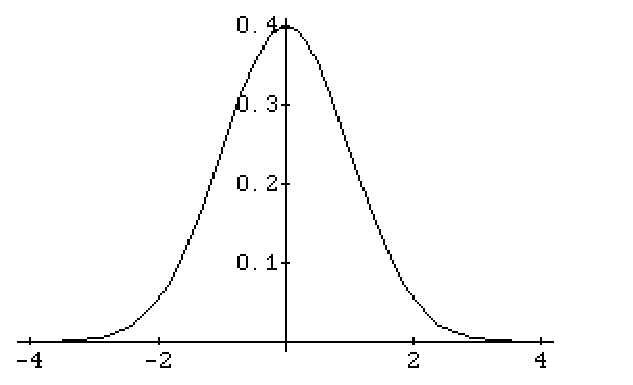
\includegraphics{normal.eps}
%%%%%%%%\end{center}
%%%%%%%%\caption{Curva de Gauss con $\mu=0$ y $\sigma=1$ }
%%%%%%%%\end{figure}



Su función de distribución es, como sabemos :
$$F(x)=\int_{-\infty}^{x} {1\over{\sqrt{2\pi}\sigma}}
{e\vphantom{A}}^{-{1\over 2}{\left({t-\mu}\over{\sigma}\right)}^{2}} dt$$

Que no tiene ninguna expresión algebraica ``decente''. Es por esta razón, y  por comodidad,
que esta función está tabulada.



Cuando una variable tiene distribución normal con parámetros $\mu,\sigma$ la denotamos por
$X\equiv N(\mu,\sigma^2)$


\subsubsection{Resumen v.a con distribución normal, $N(\mu,\sigma^2)$}

\scriptsize
\begin{tabular}{|c|c|c|c|c|}
\hline \begin{tabular}{c} Valores\\ admisibles.\end{tabular} & $f_{X}(x)$ & $F_X(x)=P(X\leq
X)=$ &
 $E(X)$ & $Var(X)$\\\hline & & & &\\
 $D_X=\RR$ & $=\frac{1}{\sqrt{2\pi}\sigma}
          e^{\frac{-(x-\mu)^2}{2\sigma^{2}}}\mbox{ para todo }x\in \R$ & Tabulada la
          $N(0,1)$ & $\mu$ & $\sigma^2$ \\& & & &\\ \hline
\end{tabular}
\normalsize



\subsubsection{Propiedades de la distribución normal.} La función de densidad de la
distribución normal tiene las siguientes propiedades:
\begin{enumerate}[a)]
\item $f$ es continua
\item $\int_{-\infty}^{+\infty} {1\over{\sqrt{2\pi}\sigma}} {e\vphantom{A}}^{-{1\over
2}{\left({x-\mu}\over{\sigma}\right)}^{2}} dx =1$ ( propiedad de todas las densidades).
\item $f(\mu+x)=f(\mu-x)$ y $F(x+\mu)=1-F(\mu-x)$ para todo $x\in \cal{R}$
\item $\lim\limits_{x\to+\infty}f(x)=\lim\limits_{x\to-\infty}f(x)=0$
es decir tiene asíntota horizontal a derecha e izquierda.
\item $f$ es estrictamente creciente si $x<\mu$ y decreciente si $x>\mu$.
\item Alcanza el máximo en $x=\mu$ y en este punto vale $f(\mu)=\frac{1}{\sqrt{2\pi}\sigma}$
\item Tiene dos puntos de inflexión en $x=\mu+\sigma$ y en $x=\mu-\sigma$.
\end{enumerate}


\subsubsection{Transformaciones lineales de variables aleatorias normales}

\begin{proposition} Sea $X\equiv N(\mu,\sigma^2)$  entonces la variable $Y=a X+b$ con
$a\not=0,b\in\cal{R}$ tiene distribución $N(a\mu+b, a^2 \sigma^2)$

En particular si  $X\equiv N(\mu,\sigma^2)$, tomando $a=\frac{1}{\sigma}$ y $b=
\frac{-\mu}{\sigma}$ la v.a. $Z={{X-\mu}\over {\sigma}}$ se distribuye $N(0,1)$.

Esta propiedad es muy importante, ya que utilizándola sólo necesitaremos tabular la
$N(0,1)$. A la función de distribución de una $Z\equiv N(0,1)$ la llamaremos $F_Z$  y a una
normal $N(0,1)$  se le denomina normal estándar. Por lo tanto si
$F_X(x)=F_Z(\frac{x-\mu}{\sigma})$.
\end{proposition}

La propiedad siguiente se desprende de las propiedades generales de una normal y nos será
muy útil en los cálculos de probabilidades de una normal.

\textbf{Propiedad} Si $Z\equiv N((0,1)$ entonces $F_{Z}(x)=1-F_{Z}(-x)$.

\begin{example} Sea $Z\equiv N(0,1)$  Calcular :
\begin{enumerate}[a)]
\item Dado $\delta>0$, $P(-\delta\leq Z \leq
\delta)=F_{Z}(\delta)-F_{Z}(-\delta)=F_Z(3)-(1-F_Z(\delta))=2 F_Z(\delta)-1$
\item $P(-4\leq Z \leq 4)=F_{Z}(4)-F_{Z}(-4)=2 F_Z(4)-1$
\item $P(-2\leq Z \leq 2)=F_{Z}(2)-F_{Z}(-2)=2 F_Z(2)-1$
\item $P(Z\leq -2)=F_Z(-2)=1-F_Z(2)$
\item $P( Z \leq 2)=F_{Z}(2)$
\item $P( Z \geq 2)=1-P(Z<2)=1-F_{Z}(2)$
\item $P( Z > 2)=1-P(Z\leq 2)=1-F_{Z}(2)$
\item $P( Z = 2)=0$
\item $P( Z \geq -2)=1-P(Z< -2)=1-F_{Z}(-2)=1-(1-F_Z(2))=F_Z(2).$
\end{enumerate}
\end{example}
    Resumiendo podemos utilizar las siguientes propiedades, $X\equiv N(\mu,\sigma)$
    \begin{itemize}
    \item  $Z$ es su variable tipificada, es decir,
    $Z=\frac{X-\mu}{\sigma}\equiv N(0,1)$ entonces:

    $$P(X\leq x)=P(\frac{X-\mu}{\sigma}\leq
    \frac{x-\mu}{\sigma})=F_{Z}(\frac{x-\mu}{\sigma})$$

   \item  Cuando tengamos un intervalo
    $$P(a<X<b)=P(\frac{a-\mu}{\sigma}<\frac{X-\mu}{\sigma}<\frac{b-\mu}{\sigma})=$$

    $$=P(\frac{a-\mu}{\sigma}<Z<\frac{b-\mu}{\sigma})=F_{Z}(\frac{b-\mu}{\sigma})-
    F_{Z}(\frac{a-\mu}{\sigma})$$
    \item Si $\delta>0$ $P(\mu-\delta\leq X \leq
\mu+\delta)=2 F_Z(\frac{\delta}{\sigma})-1$
\end{itemize}


    \begin{example}Sea $X$ una normal com media $2$ y varianza $4$, entonces
    \begin{enumerate}[a)]
\item  $P(1< X< 2)= P(\frac{1-2}{2}<\frac{X-2}{2}<\frac{2-2}{2})=
    P(\frac{-1}{2}<Z<0)=F_{Z}(0)-F_{Z}(-0.5)=\frac{1}{2}-1+F_{Z}(0.5).$
    \item $P(X>3)=P(\frac{X-2}{2}>\frac{3-2}{2})=
    P(Z>0.5)=1-F_{Z}(0.5).$
    \end{enumerate}
\end{example}
\chapter{Variables aleatorias vectoriales}
En este tema estudiaremos brevemente el comportamiento aleatorio conjunto  de varias variables. También veremos
uno de los teoremas más utilizados en estadística el Teorema del Límite central.

%%%%%%%%\textbf{Definición:} Sean $X_{1},X_{2},\ldots,X_{n}$ $n$ v.a. continuas entonces:
%%%%%%%%\begin{itemize}
%%%%%%%%    \item[i)]  su función de distribución acumulada conjunta es
%%%%%%%%    $$F_{X_{1},X_{2},\ldots,X_{n}}(x_{1},x_{2},\ldots,x_{n})=$$
%%%%%%%%    $$=P(X_{1}\leq x_{1},X_{2}\leq x_{2},\ldots,X_{n}\leq x_{n})$$
%%%%%%%%    \item[ii)]  $F_{X_{1}}(x_{1}),F_{X_{2}}(x_{2}),\ldots,F_{X_{n}}(x_{n})$
%%%%%%%%son las funciones de distribución marginales de \break $X_{1},X_{2},\ldots,X_{n}$
%%%%%%%%respectivamente.
%%%%%%%%\end{itemize}
%%%%%%%%
%%%%%%%%  \begin{itemize}
%%%%%%%%\item[iii)]  Se dice que  estas v.a. son independientes sii
%%%%%%%%$$F_{X_{1},X_{2},\ldots,X_{n}}(x_{1},x_{2},\ldots,x_{n})=$$
%%%%%%%%$$=F_{X_{1}}(x_{1})\cdot F_{X_{2}}(x_{2})\cdot\ldots \cdot
%%%%%%%%F_{X_{n}}(x_{n})$$
%%%%%%%%\item[iv)] $f(x_{1},x_{2},\ldots,x_{n})\geq 0$ es una función de densidad
%%%%%%%%de $F_{X_{1},X_{2},\ldots,X_{n}}(x_{1},x_{2},\ldots,x_{n})$ sii
%%%%%%%%
%%%%%%%%
%%%%%%%%$$F_{X_{1},X_{2},\ldots,X_{n}}(x_{1},x_{2},\ldots,x_{n})=$$
%%%%%%%%$$=\int\limits_{-\infty}^{x_{1}}\int\limits_{-\infty}^{x_{2}}
%%%%%%%%\ldots\int\limits_{-\infty}^{x_{n}} f(t_{1},f(t_{2},\ldots,t_{n}) dt_{n}\ldots
%%%%%%%%dt_{2}dt_{1}$$
%%%%%%%%\end{itemize}

\section{Variables aleatorias bidimensionales}

Vamos a exponer las nociones básicas de variables aleatorias bidimensionales.

\begin{definition}
Dadas $X$, $Y$ dos variables aleatorias, continuas o discretas, llamaremos función de distribución o de
probabilidad acumulada conjunta a:

$$ F_{X Y}(x,y)=P(X\leq x, Y\leq y).$$

La funciones de distribución de las variables $X$ e $Y$, $F_X$ y $F_Y$ reciben el nombre de
distribuciones marginales. Esta dewfinición se generaliza de forma natural a $n$ variables.
\end{definition}

\subsubsection{Independencia}

  \begin{definition}
Sean $X$, $Y$ dos variables aleatorias con función de distribución conjunta $F_{X  Y}$. Diremos que $X$, $Y$ son independientes cuando $$F_{X Y}(x,y)=F_X(x) F_Y(y).$$

Esta propiedad se generaliza a $n$ variables. Es decir $n$ variables aleatorias son independientes si su función de distribución conjunta es el producto de las  distribuciones de cada una de las variables.
  \end{definition}


\subsection{Variables aleatorias conjuntamente discretas}

\begin{definition} Sean $X$, $Y$ dos v.a. discretas. Llamaremos función de probabilidad
conjunta de $X$ , $Y$ a

$$P_{X,Y}(x,y)=P(X=x,Y=y)$$

donde $P(X=x,Y=y)=P(\{X=x\}\cap \{Y=y\})$.

Llamaremos función de probabilidad marginal de $X$ y de $Y$ a $P_X(x)$ y a $P_Y(y)$
respectivamente.
\end{definition}


\begin{proposition} Sean $X$, $Y$ dos v.a. discretas con función de probabilidad conjunta
$P_{X Y}$, entonces:

\begin{enumerate}[a)]
\item $0 \leq P_{X,Y}(x,y)\leq 1$.
\item $\sum_{x}\sum_y P_{X Y}(x,y)=1$
\item $P_X(x)=\sum_{y}P_{X Y}(x,y)$,  $P_Y(y)=\sum_{x}P_{X Y}(x,y)$.
\end{enumerate}
\end{proposition}




\begin{proposition} Sean $X$, $Y$ dos v.a. discretas con función de probabilidad conjunta
$P_{X Y}$ y función de distribución $F_{X Y}$. Entonces $$F_{X Y }(x,y)=\sum_{x_i\leq
x}\sum_{y_i\leq y} P(X=x_i,Y=y_i).$$
\end{proposition}


  \begin{proposition}
Dadas dos v.a. $X$ , $Y$ discretas con función de probabilidad conjunta $P_{XY}$. Se tiene
que  $X$ e $Y$ son independientes si y sólo si $P_{X Y}(x,y)=P_X(x) P_Y(y)$ para todo
$x,y$. Esta propiedad se generaliza a $n$ variables.
  \end{proposition}

    \begin{example}

            Supongamos que $X$ e $Y$ son las v.a. que nos dan el valor del
            lanzamiento (de forma independiente) de dos dados bien
            ba\-lan\-cea\-dos.
            Es fácil deducir que

            $$P_{XY}(i,j)=\left\{\begin{array}{ll} \frac{1}{36} & \mbox{si }
            i,j=1,2,3,4,5,6\\

            0 & \mbox{ en el resto de casos} \end{array}\right.$$

            Normalmente se disponen estos resultados en forma de tabla:

            \begin{center}\begin{tabular}{l|l|cccccc|l}
        &\multicolumn{1}{c}{}   & \multicolumn{6}{|c|}{$X$} & \\\hline
        &    & 1 & 2 & 3 & 4 & 5 & 6 & $P_{Y}$\\\hline
            & 1 & $\frac{1}{36}$ & $\frac{1}{36}$ & $\frac{1}{36}$ & $\frac{1}{36}$ &
            $\frac{1}{36}$ & $\frac{1}{36}$ & $\frac{1}{6}$\\
            &   2 & $\frac{1}{36}$ & $\frac{1}{36}$ & $\frac{1}{36}$
                & $\frac{1}{36}$ &
            $\frac{1}{36}$ & $\frac{1}{36}$ & $\frac{1}{6}$\\
        $Y$ &   3 & $\frac{1}{36}$ & $\frac{1}{36}$ & $\frac{1}{36}$
                & $\frac{1}{36}$ &
            $\frac{1}{36}$ & $\frac{1}{36}$ & $\frac{1}{6}$\\
            &   4 & $\frac{1}{36}$ & $\frac{1}{36}$ & $\frac{1}{36}$
                & $\frac{1}{36}$ &
            $\frac{1}{36}$ & $\frac{1}{36}$ & $\frac{1}{6}$\\
            &   5 & $\frac{1}{36}$ & $\frac{1}{36}$ & $\frac{1}{36}$
                & $\frac{1}{36}$ &
            $\frac{1}{36}$ & $\frac{1}{36}$ & $\frac{1}{6}$\\
            &   6 & $\frac{1}{36}$ & $\frac{1}{36}$ & $\frac{1}{36}$
                & $\frac{1}{36}$ &
        $\frac{1}{36}$ & $\frac{1}{36}$ & $\frac{1}{6}$\\\hline
        &   $P_{X}$ & $\frac{1}{6}$& $\frac{1}{6}$& $\frac{1}{6}$&
            $\frac{1}{6}$&
            $\frac{1}{6}$& $\frac{1}{6}$ & 1
            \end{tabular}
\end{center}

            En esta tabla se pueden comprobar fácilmente las propiedades
            anteriores. Además debido a la ``independencia'' en el lanzamiento
            de los dados se cumple que $P_{XY}(x,y)=P_{X}(x) P_{Y}(y)$ las variables son independientes
            y podemos ``recuperar la función de probabilidad conjunta
            conociendo las marginales''.

            Pero supongamos que los dados están bien ba\-lan\-cea\-dos pero que no
            son ``independientes''  como por ejemplo en el siguiente caso:

            \begin{center}        \begin{tabular}{l|l|cccccc|l}
        &\multicolumn{1}{c}{}   & \multicolumn{6}{|c|}{$X$} & \\\hline
        &    & 1 & 2 & 3 & 4 & 5 & 6 & $P_{Y}$\\\hline
            & 1 & $\frac{2}{42}$ & $\frac{1}{42}$ & $\frac{1}{42}$ & $\frac{1}{42}$ &
            $\frac{1}{42}$ & $\frac{1}{42}$ & $\frac{1}{6}$\\
            &   2 & $\frac{1}{42}$ & $\frac{2}{42}$ & $\frac{1}{42}$
                & $\frac{1}{42}$ &
            $\frac{1}{42}$ & $\frac{1}{42}$ & $\frac{1}{6}$\\
        $Y$ &   3 & $\frac{1}{42}$ & $\frac{1}{42}$ & $\frac{2}{42}$
                & $\frac{1}{42}$ &
            $\frac{1}{42}$ & $\frac{1}{42}$ & $\frac{1}{6}$\\
            &   4 & $\frac{1}{42}$ & $\frac{1}{42}$ & $\frac{1}{42}$
                & $\frac{2}{42}$ &
            $\frac{1}{42}$ & $\frac{1}{42}$ & $\frac{1}{6}$\\
            &   5 & $\frac{1}{42}$ & $\frac{1}{42}$ & $\frac{1}{42}$
                & $\frac{1}{42}$ &
            $\frac{2}{42}$ & $\frac{1}{42}$ & $\frac{1}{6}$\\
            &   6 & $\frac{1}{42}$ & $\frac{1}{42}$ & $\frac{1}{42}$
                & $\frac{1}{42}$ &
        $\frac{1}{42}$ & $\frac{2}{42}$ & $\frac{1}{6}$\\\hline
        &   $P_{X}$ & $\frac{1}{6}$& $\frac{1}{6}$& $\frac{1}{6}$&
            $\frac{1}{6}$&
            $\frac{1}{6}$& $\frac{1}{6}$ & 1
            \end{tabular}
\end{center}

            Aquí $P_{XY}(x,y)\not= P_{X}(x) P_{Y}(y)$.
            En este caso sabiendo las marginales no podemos
            saber la
            distribución conjunta, las variables no son independientes.

        \end{example}

        \begin{example}
              Sea $N=$ número de bytes de un mensaje, supongamos que $N$ sigue
              una distribución $Ge(1-p)$. $N$ toma valores en $\N$.
              y $P(N=n)=(1-p) p^n$. Supongamos
              que los mensajes se distribuyen en paquetes con un máximo de $M$
              bytes cada uno. Sea $C=$número de paquetes completos que ocupa
              un mensaje y sea $R=N-CM$ el número de bytes ``sobrantes''.
              \begin{enumerate}[a)] 
              \item Vamos a determinar la distribución conjunta de $C$ y $R$ es decir
              del vector aleatorio bidimensional $(C,R)$.

              Si el mensaje tiene $N$ bytes entonces sea
             $N=MC+R$ la división entera de $N$ por $M$, sabemos que
             $0\leq R\leq M-1$ es decir $R\in\{0,1,2,..,M-1\}$ y por lo tanto
             si $c\in\N$ y $r\in\{0,1,2,..,M-1\}$ entonces:

             $$P(C=c,R=r)= P(N=cM+r)=(1-p) p^{cM+r}.$$

             Luego $P_{CR}(c,r)=(1-p) p^{cM+r}$ con $c\in N$ y $0\leq r\leq
             M-1$ siendo cero en el resto de casos.

             \item Calculemos las funciones de probabilidad marginales.

             $$P_{C}(c)=P(C=c)=\sum_{r=0}^{M-1} P_{CR}(c,r)=\sum_{r=0}^{M-1}(1-p) p^{cM+r}=
             (1-p) p^{cM} \sum_{r=0}^{M-1} p^r=$$
             $$ (1-p)
             p^{cM}\frac{1-p^{M-1}p}{1-p}=(1-p^M) {(p^M)}^{c} c=0,1,2,\ldots$$

             Luego $C$ es una $Ge(1-p^{M})$.

             De forma similar $P_{R}(r)=\frac{1-p}{1-p^M} p^r$ para
             $r=0,1,\ldots,M-1$

             \item ¿Son las variables $C$ y $R$ independientes?  Lo serán si el producto de las marginales es igual a la conjunta? Esto sucederá si el cociente $C$ es independiente del resto $R$
             como sucesos. Efectivamente:

             $P_{C}(c) P_{R}(r)=(1-p^M) {(p^M)}^{c} \frac{1-p}{1-p^M} p^r=
             (1-p) p^{cM+r}=P_{CR}(c,r)$ y por lo tanto $C$ y $R$ son independientes.
\end{enumerate}
\end{example}

\subsection{Variables aleatorias bidimensionales continuas}

\begin{definition}

Una función $f:\R^2\to R$ es una función de densidad bidimensional si es no negativa,  es
integrable en $R^2$ y $\int_{-\infty}^{\infty}\int_{-\infty}^{\infty} f(x,y) dx dy=1$

\end{definition}

\begin{definition}

Dadas dos v.a. continuas $X$ e $Y$ diremos que son conjuntamente continuas si existe una
función de densidad $f_{X Y}:\R^2\to \R$ tal que

$$F_{X Y}(x,y)=\int_{-\infty}^{x} \int_{-\infty}^{y} f_{X Y}(u,v) d v du$$

\end{definition}

\begin{definition}
Dadas dos v.a. $X$ e $Y$ conjuntamente continuas las funciones de densidad y de
distribución de $X$ e $Y$ reciben el nombre de densidades y distribuciones marginales.
\end{definition}



             \begin{proposition}
Se verifican las siguientes propiedades:

              \begin{enumerate}[a)]
              \item $\displaystyle P((X,Y)\in A)=\int\int_{A} f_{XY}(x,y) dx dy$
             %%%%%%%% \item  $\displaystyle \int_{-\infty}^{+\infty}\int_{-\infty}^{+\infty}
%%%%%%%%              f_{XY}(x,y) dx dy=$\newline $\displaystyle =\int\int_{\R^{2}} f_{XY}(x,y) dx dy=1$
              \item 
              \footnote{ Esta propiedad se verifica salvo en un conjunto
              de ``medida nula'', es decir de probabilidad $0$.
                  Al igual que en el caso discreto no siempre es posible
                  obtener la distribución o la densidad conjunta desde las
                  marginales.} $f_{XY}(x,y)=\frac{\partial^2 }{\partial x \partial y}
              F_{XY}(x,y)$
              \item $\displaystyle f_{X}(x)=\int_{-\infty}^{+\infty} f_{XY}(x,y) dy$;
              $\displaystyle f_{Y}(y)=\int_{-\infty}^{+\infty} f_{XY}(x,y) dx$.
              \end{enumerate}
\end{proposition}

\begin{example}
              Distribución uniforme en un recinto. Sea $R$ un ``recinto''
              adecuado del plano. Sean $(X,Y)$ las coordenadas resultantes de elegir al
              azar un punto de ese recinto y sea $A$= área del recinto $R$.
              Entonces diremos que $(X,Y)$ sigue una ley uniforme en ese
              recinto si su función de densidad es

              $f_{XY}(x,y)=\left\{
                            \begin{array}{ll}
                  \frac{1}{A} & \mbox{si } (x,y)\in R  \\
                 0 & \mbox{en cualquier otro caso}
              \end{array}\right.$

              En particular si $R=(a,b)^2$ entonces $(X,Y)$ siguen una ley
              uniforme en rectángulo $(a,b)^2$ si su densidad
              es

              $f_{XY}(x,y)=\left\{
                            \begin{array}{ll}
                  \frac{1}{(b-a)^2} & \mbox{si } a< x,y< b\\
                 0 & \mbox{en cualquier otro caso}
              \end{array}\right.$


              Es fácil comprobar que las marginales de esta última
              distribución conjunta son uniformes en $(a,b)$.

              Ejercicio; Construir la densidad de $(X,Y)$  
              uniforme sobre los recintos $R=(a,b)\times(c,d)$ y $R=\{(x,y)|
              x^2+y^2\leq r^2\}$ con $r>0$
             \end{example}
     \begin{example}
                  Consideremos una diana cuadrada $(0,1)\times (0,1)$.
                  Sean $(X,Y)$ las coordenadas de un impacto ``al azar
                  en esta diana''.
                  
                  Al ser al azar la probabilidad de un suceso
                  será igual al cociente
                  $$
                  \frac{\mbox{área total favorable}}{\mbox{área
                  total posible}}$$
                  
                  entonces si $0<x<1$ y $0<y<1$

                  $P(X\leq x , Y\leq y)=xy$

                  Pero si $0<x<1$ y $1\leq y$ entonces

                  $P(X\leq x, Y\leq y)=P(X\leq x , Y\leq 1)=P(X\leq x)=x$

                  Análogamente si $1\leq x$ $0<y<1$ tenemos que

                  $P(X\leq x,Y\leq y)=y$

                  En resumen completando los casos que faltan resulta que la
                  función de distribución conjunta es:

                  $F_{XY}(x,y)=\left\{
                     \begin{array}{ll}
                      0 & \mbox{si } x<0 \mbox{ ó } y<0  \\
                     xy & \mbox{si } 0\leq x\leq 1 \mbox{ y } 0\leq y\leq 1   \\
                      x & \mbox{si } 0\leq x\leq 1 \mbox{ y } y>1\\
                      y & \mbox{si } 0\leq y\leq 1 \mbox{ y } x>1  \\
                      1 & \mbox{si } x>1 \mbox{ y } y>1
                  \end{array}
             \right.$


         Entonces la densidad
                     \footnote{ Notemos que
                 $\frac{\partial^2}{\partial x \partial y} F_{XY}(x,y)$ no existe
                 en los bordes del cuadrado que forman un conjunto de
                 medida nula.} de $F_{XY}$ es

        $f_{XY}(x,y)=$\newline$\frac{\partial^2}{\partial x \partial y} F_{XY}(x,y)=
        \left\{
                                        \begin{array}{ll}
                      1 & \mbox{si } 0\leq x\leq 1 \mbox{ y } 0\leq y\leq 1  \\
                     0 & \mbox{ en otro caso}
                 \end{array}\right.$

                Ahora es fácil comprobar que

                $\displaystyle F_{XY}(x,y)=\int_{-\infty}^{x}\int_{-\infty}^{y} f_{XY}(u,v)du
                dv$

                También es fácil ver que en este caso el producto de las densidades
                (distribuciones)  mar\-gi\-na\-les es igual a la densidad (distribución)
                conjuntas.

                \end{example}
                \begin{example}
                \begin{enumerate}[a)]
                  Encontrar el valor de $c$ para que

                  $f_{XY}(x,y)=\left\{
                   \begin{array}{ll}
                      c e^{-x} e^{-y} & \mbox{si } 0\leq y\leq x   \\
                      0 & \mbox{en otro caso}
                  \end{array}\right.$

                  Sea función de densidad.

                  Al igual que en el caso unidimensional es suficiente con que
                  la función sea integrable, no negativa e integre 1 en $\R^2$.
                 Las dos primeras condiciones son evidentes (si $c>0$), veamos la última:

                 $\displaystyle
                 \int_{-\infty}^{+\infty}\int_{-\infty}^{+\infty} f_{XY}(x,y)
                 dx dy=1$ y como
                 $\displaystyle\int_{0}^{+\infty}\int_{0}^{x}  e^{-x} e^{-y} dy dx=
                 \frac{1}{2}$

                 entonces $c=2$. Luego
                 $f_{XY}(x,y)=\left\{
                   \begin{array}{ll}
                      2 e^{-x} e^{-y} & \mbox{si } 0\leq y\leq x   \\
                      0 & \mbox{en otro caso}
                  \end{array}\right.$

                  \item Las densidades marginales serán:
                  
                  $$ f_{X}(x)=\int_{0}^{+\infty} f_{XY}(x,y) dy=
                  \int_{0}^{x} 2 e^{-x} e^{-y} dy= 2 e^{-x} (1-e^{-x})$$

                  si $x\geq 0$ y cero en cualquier otro caso.

                  De forma análoga:$f_{Y}(y)=2 e^{-2y}$ si $0\leq y$, siendo cero en cualquier
                  otro caso.

                  \item Calculemos ahora $P(X+Y\leq 1)$.
                  Sea $A$ el conjunto de puntos del plano tales que $X+Y\leq 1$
                  entonces:\newline
                  $\displaystyle P(X+Y\leq 1)=
                  \int\int_{A} f_{XY}(u,v) dudv=$\newline
                  $\displaystyle =\int_{y=0}^{\frac{1}{2}} \int_{x=y}^{1-y} 2 e^{-x}
                  e^{-y} dx dy=
                  1-2 e^{-1}$
                  
                  \end{enumerate}
\end{example}

 

  

\subsection{Distribuciones condicionales. (OPCIONAL)}


    Sea $(X,Y)$ una v.a. bidimensional discreta. Estudiemos la v.a.
    $X/Y=y$.

    \begin{definition}    Sea $(X,Y)$ una v.a. bidimensional discreta con función de
    probabilidad conjunta $P_{XY}(x,y)$. Sea $y$ tal que $P(Y=y)>0$.
    De\-fi\-ni\-mos la función de probabilidad de $X$ condicionada a que $Y=y$
    como $$P_{X}(x|y)=P(X=x/ Y=y)$$ para todo $x\in\R$.

    $X/Y=y$ resulta ser una v.a. discreta que tiene por función de probabilidad
    $P_{X}(x|y)$

    Análogamente dado $x$ tal que $P(X=x)>0$ definimos
      $Y/X=x$ que tiene por función de probabilidad $P_{Y}(y|x)=P(Y=y/
      X=x)$ para todo $y\in\R$

      \end{definition}

    \begin{proposition}
      Sean $X$ e $Y$ dos v.a. discretas.
      Enunciamos las siguientes propiedades para $X/Y=y$,
      se enuncian de
      forma similar para $Y/X=x$
 \begin{enumerate}[a)]
        \item$\sum_{x} P_{X}(x|y)=1$. Efectivamente
          $$\sum_{x} P_{X}(x|y)=\sum_{x}
          P(X=x/Y=y)=$$
          $$=\sum_{x}\frac{P(X=x,Y=y)}{P(Y=y)}=
          \sum_{x}\frac{P_{XY}(x,y)}{P_{Y}(y)}=$$
          $$=\frac{1}{P_{Y}(y)}\sum_{x}P_{XY}(x,y)=
          \frac{P_{Y}(y)}{P_{Y}(y)}=1$$
    \item $P_{X}(x|y)=\frac{P_{XY}(x,y)}{P_{Y}(y)}=
          \frac{P_{XY}(x,y)}{\sum_{x}P_{XY}(x,y)}$

         Luego es suficiente conocer la distribución conjunta para
         calcular la condicional.
         \item $F_{X}(x_{0}|y)=P(X\leq x_{0}/Y=y)=\sum_{x\leq x_{0}}P_{X}(x|y)$

\item$P_{XY}(x,y)=P_{Y}(y) P_{X}(x|y)$. Luego podemos
         calcular la función de probabilidad conjunta a partir de la
         marginal y la condicional.

      \item $X$ es independiente de $Y$ sii
         $P_{X}(x|y)=P_{X}(x)$ para todo $x,y$.
\end{enumerate}
\end{proposition}

\begin{example}
 Un técnico tiene que revisar un sistema de dispositivos. No los revisa todos cada vez
sino que escoge el número a revisar de forma equiprobable entre 5 y 8. Sea $X$= número de
dispositivos que revisa el técnico. Sabiendo que $X=x$ dispositivos el tiempo en segundos
que el técnico tarda en revisarlos es una v.a. $Y$ (discreta) con función de probabilidad

$P_{Y}(y|x)=\frac{10-x}{x} \left(\frac{x}{10}\right)^y$ para $y=1,2,3\ldots$ y cero en el
resto de casos.

Entonces

$P_{XY}(x,y)=P_{X}(x) P_{Y}(y|x)=\frac{1}{4}\frac{10-x}{x} \left(\frac{x}{10}\right)^y$

para $y=1,2,3,\ldots$; $x=5,6,7,8$

Calculemos la marginal de $Y$ desde la conjunta $$P_{Y}(y)=\sum_{x=5}^{8}
P_{XY}(x,y)=\sum_{x=5}^{8} \frac{1}{4}\frac{10-x}{x}
\left(\frac{x}{10}\right)^y=\frac{1}{4\cdot10^{y}}\sum_{x=5}^{8} (10-x) x^{y-1}$$


También podemos calcular la marginal de $X$:
$$ P_{X}(x)=\sum_{1\leq y}f_{XY}(x,y)=
\sum_{1\leq y} \frac{1}{4} \frac{10-x}{x} \left(\frac{x}{10}\right)^y=$$
$$\frac{10-x}{4x}
\sum_{1\leq
y}\left(\frac{x}{10}\right)^{y}=\frac{10-x}{4x}\left(\frac{1}{1-\frac{x}{10}}-1\right)=$$

$\displaystyle{=\frac{10-x}{4x}\frac{10-(10-x)}{10-x}=\frac{1}{4}}$
\end{example}




\subsubsection{Variables condicionadas a un suceso}

Tambien podemos condicionar una variable a un suceso.

\begin{definition}
\textbf{Definición}  Sea $(X,Y)$ una v.a. bidimensional discreta  y sea $B$ un conjunto del plano tal que
$P((X,Y)\in B)>0$. Definimos la función de probabilidad de $X$ condicionada al suceso
$\{(x,y)\in B\}$ como

$P_{X}(x|B)=P(X=x/(X,Y)\in B)$
\end{definition}


\begin{example}
Consideremos un canal de comunicación sea $(X,Y)$ una v.a. donde $X$=símbolo emitido,
$Y$=símbolo recibido. La función de probabilidad conjunta $P_{XY}$ viene determinada por la
siguiente tabla:

\begin{center}\begin{tabular}{c|c|ccc|c}
   \multicolumn{2}{c|}{}  & \multicolumn{3}{|c|}{$Y$}  & \\
    \cline{3-6}
    \multicolumn{2}{c|}{} & 1 & 2 & 3 & $P_{X}$ \\
    \hline
     & 1 & 0.1 & 0.2 & 0.1 & 0.4  \\
    $X$ & 2 & 0.2 & 0.1 & 0 & 0.3  \\
   & 3 & 0.1 & 0.2 & 0 & 0.3  \\
   \cline{2-6}
     & $P_{Y}$ & 0.4 & 0.5 & 0.1 & 1  \\
    \hline
\end{tabular}
\end{center}


Consideremos el suceso ``error'' \newline
$E=\{(1,2),(1,3),(2,1),(2,3),(3,1),(3,2)\}$.\newline Que también se puede expresar como
$X\not=Y$. Entonces $P((X,Y)\in E)=1-P((X,Y)\not\in E)=1- 0.1-0.1-0=0.8$



Queremos calcular la función de probabilidad de $Y$ condicionado a error.

$P_{Y}(y|X\not=Y)=P(Y=y/(X,Y)\in E)=$

$\frac{P(Y=y\cap \{(X,Y)\in E\}}{P((X,Y)\in E)}=\frac{P((X,y)\in \{(x,y)|x\not= y\})}{0.8}$

Entonces

$P_{Y}(1|X\not=Y)=\frac{P((X,1)\in \{(x,1)|x\not= 1\})}{0.8}=$\newline $=\frac{P((X,1)\in
\{(2,1),(3,1)\})}{0.8}=\frac{3}{8}$

$P_{Y}(2|X\not=Y)=\frac{P((X,2)\in \{(x,2)|x\not= 2\})}{0.8}=$\newline $=\frac{P((X,2)\in
\{(1,2),(3,2)\})}{0.8}=\frac{4}{8}$

$P_{Y}(3|X\not=Y)=\frac{P((X,3)\in \{(x,3)|x\not= 3\})}{0.8}=$\newline $=\frac{P((X,3)\in
\{(1,3),(2,3)\})}{0.8}=\frac{1}{8}$
\end{example}


\textbf{Nota:} En este caso las funciones de distribución condicionadas se pueden calcular así
$$F_{X}(x_{0}|(x,y)\in B)=P(X\leq x_{0}/(x,y)\in B)=\sum_{x\leq
x_{0}}P_{X}(x|(x,y)\in B)$$




%                 \textbf{Ejemplo}
%
%                 Sea $-1\leq \pho\leq 1$ una constante real. Consideremos la
%                 siguiente función:
%
%                 $f_{XY}=\frac{1}{2\pi \sqrt{1-\pho} e ^{-\frac{x^2 -2\rho xy
%                 +y^2}{2(1-\rho^2)}}$
%
%                 Esta función es una densidad, es la función de densidad
%                 gaussiana bivariante o normal bivariante.

            

\begin{definition}
    Sea $(X,Y)$ una v.a. bidimensional conjuntamente
    continua y sea $y$ un valor ``posible'' de $Y$, es decir,
    $f_{Y}(y)>0$. Definimos la función de distribución de $X$
    condicionado a que $Y=y$, la variable $X/Y=y$,como

    $F_{X}(x|y)=\lim_{h\to 0} P(X\leq x/y\leq Y\leq y+h)$.

    Llamaremos función de densidad condicionada de $X$ a que $Y=y$ a la función de densidad
    de la variable $X/Y=y$ y la denotaremos por $f_{X}(x/y)$.
\end{definition}

    Justifiquemos la definición. En primer lugar es claro que no
    podemos proceder como en el caso discreto pues al ser la v.a.
    continua $P(Y=y)=0$.

    Por otra parte
    $$\displaystyle{P(X\leq x/y\leq Y\leq y+h)=}$$

   $$\displaystyle{=\frac{P(\{X\leq x\}\cap \{y\leq
    Y\leq y+h\})}{P(y\leq Y\leq y+h)}}$$

    entonces
       $ F_{X}(x|y)=\frac{\lim_{h\to 0}P(\{X\leq x\}\cap \{y\leq
    Y\leq y+h\})}{\lim_{h\to 0}P(y\leq Y\leq y+h)}$

    Al ser las variables continuas
    $\displaystyle{\lim_{h\to 0}P(\{X\leq x\}\cap \{y\leq
    Y\leq y+h\})=}=P(X\leq x,Y= y)=0$

    $\displaystyle{\lim_{h\to 0}P(y\leq Y\leq y+h)=P(Y=y)=0}$

    Luego el cociente está indeterminado. Pero este límite
    existe  pues:

    $F_{X}(x|y)=\lim_{h\to 0}\frac{P(\{X\leq x\}\cap \{y\leq
    Y\leq y+h\})}{P(y\leq Y\leq y+h)}=$\newline
$=\lim_{h\to 0}\frac{F_{XY}(x,y+h)-F_{XY}(x,y)}
    {F_{Y}(y+h)-F_{Y}(y)}=$\newline
    $=\lim_{h\to 0}\frac{\frac{F_{XY}(x,y+h)-F_{XY}(x,y)}{h}}
    {\frac{F_{Y}(y+h)-F_{Y}(y)}{h}}=\frac{\frac{\partial F_{XY}(x,y)}{\partial
    y}}{f_{Y}(y)}$

    Lo que demuestra la existencia de la distribución condicionada
    y la siguiente propiedad, que no servirá para el  cálculo de las distribuciones
    condicionales de variables aleatorias conjuntamente continuas.

   \begin{proposition}
   Con las notaciones y condiciones  anteriores se tiene que: 

   \begin{enumerate}[a)]
   \item $F_{X}(x|y_0)=\left[\frac{\frac{\partial F_{XY}(x,y)}{\partial y}}{f_{Y}(y)}\right]_{y=y_0}$

Además  $\frac{\partial}{\partial x} F_{X}(x|y)=f_{X}(x|y)$ y por lo tanto   $F_{X}(x|y)$
es una auténtica función de distribución.
 \item $f_X(x/y)=\frac{f_{X Y}(x,y)}{f_y{y}}$.
\end{enumerate}
 \end{proposition}
 Efectivamente:

$\frac{\partial}{\partial x} F_{X}(x|y)=\frac{\frac{\partial^2}{\partial x\partial
y}F_{XY}(x,y)}{f_{Y}(y)}=\frac{f(x,y)}{f_{Y}(y)}=f_{X}(x|y)$

Además como $\frac{f(x,y)}{f_{Y}(y)}>0$ deducimos que $F_{X}(x|y)$ es creciente.

Por otra parte $F_{X}(+\infty|y)=\frac{\frac{\partial}{\partial
y}F_{XY}(+\infty,y)}{f_{Y}(y)}=\frac{\frac{d}{d
y}F_{Y}(y)}{f_{Y}(y)}=\frac{f_{Y}(y)}{f_{Y}(y)}=1$

De forma similar $F_{X}(-\infty|y)=0$

Estos últimos resultados junto a que $F_{X}(x|y)$ es creciente en $x$ implican que $0\leq
F_{X}(x|y)\leq 1$.

Por último al ser $F_{X}(x|y)$ derivable es continua.



    \textbf{Observaciones}

    \begin{enumerate}[a)]
    \item Algunos resultados anteriores son  similares a los de v.a.
    discretas cambiando las funciones de probabilidad por las densidades.
    \item $f_{XY}(x,y)=f_{Y}(y) f_{X}(x|y)$ si $f_{Y}(y)>0$
    \item Si queremos calcular $F_{X}(x|(x,y)\in B)$ donde $B$ es una
    región (adecuada) del plano y $P((x,y)\in B)>0$ podemos definir

    $F_{X}(x|(x,y)\in B)=P(X\leq x/(x,y)\in B)$

    Una vez calculada la distribución podemos derivar para obtener la
    densidad.
    \item Todo lo dicho (cambiando $X$ por $Y$) es válido para $Y/X=x$,
    $F_{Y}(y|x)$ y $f_{Y}(y/x)$.
    \end{enumerate}


    \begin{proposition}
    Sean $X$ e $Y$ dos v.a. conjuntamente continuas con función de densidad conjunta
    $f_{XY}$ entonces  $X$ e $Y$ son independientes si y sólo si $f_{X Y}(x,y)=f_{X}(x)
    f_Y(y)$ para todo $x,y$.
    \end{proposition}




\begin{example}

    Sea $X$= demanda en tiempo de un servicio; $X>0$. Sea $Y$=coste aleatorio
    del servicio; $10\leq Y\leq 15$

    Supongamos que $(X,Y)$ es una v.a. continua con densidad

    $f_{XY}(x,y)=\left\{\begin{array}{ll} \frac{1}{5} y e^{-xy} &
    \mbox{si } x>0, 10\leq y\leq 15\\
    0 & \mbox{en otro caso}\end{array}\right.$

    Queremos calcular la probabilidad de que la demanda supere 100
     cuando el coste $Y$ es $12$.
    Calculemos en primer lugar la densidad condicionada:

    $f_{X}(x|12)=\frac{f_{XY}(x,12)}{f_{Y}(12)}$
%     \end{slide}
%     \begin{slide}
    Necesitamos la densidad de $Y$

    $f_{Y}(y)=\int_{0}^{+\infty} \frac{1}{5} y e^{-xy}
    dx=$\newline
$=\left.-\frac{1}{5}e^{-xy}\right|_{0}^{+\infty}=\frac{1}{5}$
    si $10\leq y\leq 15$ y cero en el resto de casos.

    Entonces $f_{X}(x|12)=\left\{\begin{array}{ll} 12 e^{-12x} &
    \mbox{si } x>0\\
    0 & \mbox{en otro caso}\end{array}\right.$

    Por lo tanto la probabilidad pedida es \newline
    $P(X>100/Y=12)=1-F_{X}(100|12)=
    1-\int_{0}^{100} 12 e^{-12x} dx =1- \left[(-e^{-12
    x})\right]_{0}^{100}=1+e^{-1200}-1= e^{-1200}$

    Calculemos en general $F_{XY}(x,y)$

    Si $x<0$ ó $y<10$ es fácil ver que
    $F_{XY}(x,y)=0$.

    Si $0\leq x$ y $10\leq y\leq15$

    $\displaystyle F_{XY}(x,y)=\int_{10}^{y}\int_{0}^{x} \frac{1}{5} v
    e^{-uv}du dv=\newline =-\frac{1}{5x}
   \left(e^{-10x}-e^{-x y}\right)+\frac{1}{5}(y-10)$

%REPPETIR
%     \newline
%     $\int_{0}^{y} \left[-\frac{1}{5} e^{-u v}\right]_{u=0}^{x} dv=
%     -\frac{1}{5}\int_{0}^{y} \left(e^{-xv}-1\right) dv=
%     -\frac{1}{5} \left[ -\frac{e^{-x v}}{x} -v\right]_{v=0}^y=
%     \frac{1}{5} \left(\frac{e^{-xy} -1}{x}+y\right)

    Si $0\leq x$; $y\geq 15$\newline
    $F_{XY}(x,y)=1-\frac{1}{5x}\left(e^{-10x}-e^{-15x}\right)$

    En resumen:

    $F_{XY}(x,y)=$\newline$\left\{\begin{array}{ll}
    0 &  \mbox{si } y<10, \mbox{ ó } x<0\\
 \scriptstyle{ -\frac{1}{5x}
    \left(e^{-10x}-e^{-x y}\right)+\frac{1}{5}(y-10) }& \mbox{si } x<0,
   10<y<15\\
   1-\frac{1}{5x}\left(e^{-10x}-e^{-15x}\right)& \mbox{si } 0\leq x,
   y\geq 15
  \end{array}\right.$

  Ahora para comprobar si el resultado es correcto calculamos la
  parcial segunda respecto de $x$ y de $y$

  $f_{XY}(x,y)=\frac{\partial^2}{\partial x\partial y}
  F_{XY}(x,y)=$\newline
$=  \left\{\begin{array}{ll}
    0 &  \mbox{si } y<10, \mbox{ ó } (y>15, x<0)\\
   \frac{1}{5} y e^{-xy} & \mbox{si } x<0,
   10<y<15\\
  0 & \mbox{si } 0\leq x,
   y\geq 15
  \end{array}\right.$
\end{example}

\begin{example}  Consideremos la v.a. $(X,Y)$ con función de densidad conjunta


$f_{XY}(x,y)=\left\{\begin{array}{ll} \frac{1}{24} (x+y)&\mbox{si } 0<x<4, 0<y<2 \\ 0 &
\mbox{en otro caso}\end{array}\right.$

Si $0<x<4$ $f_{X}(x)=$\newline $=\int_{0}^2\frac{1}{24} (x+y) dy=\left[\frac{1}{24}(xy
+\frac{y^2}{2})\right]_{y=0}^2=\newline =\frac{x+1}{12}$

De forma análoga calculamos $f_{Y}(y)$. En resumen tenemos que:


$f_{X}(x)=\left\{\begin{array}{ll} \frac{1}{12} (x+1)&\mbox{si } 0<x<4 \\ 0 & \mbox{en otro
caso}\end{array}\right.$
\newline
$f_{Y}(y)=\left\{\begin{array}{ll} \frac{1}{6} (y+2) & \mbox{si }  0<y<2 \\ 0 & \mbox{en
otro caso}\end{array}\right.$

Vamos a calcular $f_{Y}(y|3)$, $F_{Y}(y|3)$,la pro\-ba\-bi\-li\-dad de que $Y$ esté entre 1
y 2 cuando $X=3$, $F_{XY}(x,y)$ y $F_{X}(x|X>2Y)$.


$f_{Y}(y|3)=\frac{f_{XY}(3,y)}{f_{X}(3)}=
\frac{\frac{1}{24}(3+y)}{\frac{3+1}{12}}=\frac{3+y}{8}$

si $0<y<2$ y vale cero en el resto de casos.

$F_{Y}(y|3)=\int_{0}^y \frac{3+v}{8}dv= \left[
\frac{1}{8}(3v+\frac{v^2}{2})\right]_{0}^y=\frac{1}{8}(3y+\frac{y^2}{2})$

si $0<y<2$ valiendo $0$ si $y\leq 0$ y $1$ si $y\geq 2$.

$P(1\leq Y\leq 2/X=3)=F_{Y}(2|3)-F_{Y}(1|3)= \frac{9}{16}$


Para calcular $F_{XY}$ basta integrar en los si\-gui\-en\-tes casos $f_{XY}$, obteniéndose
que

$F_{XY}(x,y)=\left\{\begin{array}{ll} 0 & \mbox{si } x\leq 0\mbox{ ó } y\leq 0\\
\frac{1}{48} xy(x+y) & \mbox{si } \scriptstyle{0< x<4,0<y<2}\\ \frac{1}{24} (x^2+2x) &
\mbox{si } 0< x<4,2\leq y\\ \frac{1}{12} (y^2+4y) & \mbox{si } 4\leq x,0<y<2\\ 1 & \mbox{si
} 4\leq x,2\leq y\\
\end{array}\right.$

Ahora podemos comprobar si la distribución  condicional calculada es correcta

$F_{Y}(y|3)=\frac{\left.\frac{\partial}{\partial x}
F_{XY}(x,y)\right|_{x=3}}{f_{X}(3)}=$\newline $=\left\{\begin{array}{ll} 0 & \mbox{si }
y\leq 0\\ \frac{3}{48}(6y +y^2) & \mbox{si } 0<y<2\\ \frac{\frac{1}{24}(2\cdot 3
+2)}{\frac{1}{3}}=1 & \mbox{si }  y\geq 2
\end{array}
\right.$

Simplificando obtenemos la misma función.

Por último:

$F_{X}(x|X>2 Y)=P(X\leq x/X>2y)=\newline =\frac{P(X\leq x,X>2Y)}{P(X>2Y)}$


Ayudándose de algún gráfico (o de forma \newline analítica) obtenemos  que

$P(X>2Y)=\int_{0}^{4}\int_{0}^{\frac{u}{2}} \frac{1}{24} (u+v) dv du=\frac{5}{9}$

$P(X\leq x , X>2Y)=\int_{0}^{x}\int_{0}^{\frac{u}{2}} \frac{1}{24}(u+v) dv du=\int_{0}^x
\frac{5 v^2}{192}du= \frac{5 x^3}{576}$

Por lo tanto

$F_{X}(x|X>2Y)=\left\{\begin{array}{ll} 0 & \mbox{si } x\leq 0\\ \frac{x^3}{64} & \mbox{si
} 0<x<4\\ 1 & \mbox{si } x\geq 4
\end{array}
\right.$

Derivando la función anterior obtenemos la densidad condicional

$f_{X}(x|X>2 Y)=\left\{\begin{array}{ll} \frac{3x^2}{64} & 0<x<4\\ 0 & \mbox{en otro caso}
\end{array}\right.$
\end{example}

    \textbf{Observaciones}
\begin{enumerate}[a)]
    \item Si $A$ es un suceso entonces
    $P(Y\in A/X=x)=\int_{A}f_{Y}(y|x) dy$.

   \item Si $X$, $Y$ son independientes entonces
\begin{itemize}
    \item $F_{Y}(y|x)=P(Y\leq y)=F_{Y}(y)$

   \item $f_{Y}(y|x)=\frac{d}{dy} F_{Y}(y|x)=f_{Y}(y)$
\end{itemize}
\end{enumerate}
%%%%%%%%    \textbf{Propiedad}
%%%%%%%%
%%%%%%%%    Si $X$ es discreta e $Y$ es absolutamente con\-ti\-nua.
%%%%%%%%
%%%%%%%%    $P(X=x)=\int_{-\infty}^{+\infty} P(X=x/Y=y) f_{Y}(y) dy
%%%%%%%%    =\int_{-\infty}^{+\infty} f_{X}(x|y) f_{Y}(y) dy$
%%%%%%%%
%%%%%%%%    $P(Y\leq y )=\sum_{x} P(Y\leq y/X=x) P(X=x)=\sum_{x} F_{Y}(y|x)
%%%%%%%%    f_{X}(x)$
%%%%%%%%    \end{slide}
%%%%%%%%\begin{slide}

 %%%%%%%% \section{Distribuciones condicionales}
%%%%%%%%
%%%%%%%%  Sean $X,Y$ dos v.a. continuas con función de densidad $f_{X Y}$ y
%%%%%%%%  función de distribución $F_{X Y}$.
%%%%%%%%
%%%%%%%%  Definimos la función de \emph{densidad condicional} de  $Y/X=x$ como
%%%%%%%%
%%%%%%%%  $f_{Y/X}(y|x)= \frac{f_{X Y}(x,y)}{f_{X}(x)}$ siempre que $f_{X}(x)>0$.
%%%%%%%%
%%%%%%%%
%%%%%%%%  Análogamente la densidad condicional de $X/Y=y$ será:
%%%%%%%%
%%%%%%%%   $f_{X/Y}(x|y)= \frac{f_{X Y}(x,y)}{f_{Y}(y)}$ siempre que $f_{Y}(y)>0$.
%%%%%%%%
%%%%%%%%  \textbf{Propiedad}
%%%%%%%%
%%%%%%%%  $f_{Y/X}(y|x)$ y  $f_{X/Y}(x|y)$ son funciones de densidad.
%%%%%%%%
%%%%%%%%
%%%%%%%%
      \begin{example}
      Sean $X, Y$ dos v.a. continuas tal que su función de densidad sea
      $$f_{XY}(x,y)=\left\{\begin{array}{ll}
      \frac{1}{2} & \mbox{ si } -a<x<a, -a<y<a\\
      0 & \mbox{en el resto de casos}
      \end{array}\right.$$

      \begin{enumerate}[a)]
          \item Encontrar el valor de $a$.
          \item Encontrar las densidades marginales de $X$ e $Y$.
          \item Encontrar $F_{X Y}$.
          \item Calcular $E(X)$ y $E(Y)$.
          \end{enumerate}
         \end{example}

     a) Se puede hacer gráficamente.

    De forma analítica tenemos:

    $1=\int_{-\infty}^\infty\int_{-\infty}^\infty f_{XY}(x,y) dx dy=
    \int_{-a}^a\int_{-a}^a \frac{1}{2} dx dy=  \int_{-a}^a
    [\frac{x}{2}]_{-a}^a dy = \int_{-a}^a dy = [a y ]_{-a}^a = a a -
    a (-a )= 2 a ^2$

    entonces $1=2a^2$ de donde $a=\frac{\sqrt{2}}{2}$, luego :

      $f_{XY}(x,y)=\left\{\begin{array}{ll}
      \frac{1}{2} & \mbox{ si } -\frac{\sqrt{2}}{2}<x<\frac{\sqrt{2}}{2},
      -\frac{\sqrt{2}}{2}<y<\frac{\sqrt{2}}{2}\\
      0 & \mbox{en el resto de casos}
      \end{array}\right.$

    b) Sea $x$ tal que $-\frac{\sqrt{2}}{2}<x<\frac{\sqrt{2}}{2}$
    entonces

    $f_{X}(x)=\int_{-\infty}^{\infty} f_{XY}(x,y) dy =
    \int_{-\frac{\sqrt{2}}{2}}^{\frac{\sqrt{2}}{2}}
    \frac{1}{2} dy = \frac{\sqrt{2}}{2}.$

    Si $x\not\in (-\frac{\sqrt{2}}{2},\frac{\sqrt{2}}{2})$ entonces
    $f_{XY}(x,y)=0$ para cualquier $y$, por lo tanto $f_{X}(x)=0$

    En definitiva:

    $f_{X}(x)=\left\{\begin{array}{ll}
      \frac{\sqrt{2}}{2} & \mbox{ si } -\frac{\sqrt{2}}{2}<x<\frac{\sqrt{2}}{2}
      \\
      0 & \mbox{en el resto de casos}
      \end{array}\right.$

      De forma análoga:

       $f_{Y}(y)=\left\{\begin{array}{ll}
      \frac{\sqrt{2}}{2} & \mbox{ si } -\frac{\sqrt{2}}{2}<y<\frac{\sqrt{2}}{2}
      \\
      0 & \mbox{en el resto de casos}
      \end{array}\right.$


      \emph{Notemos que:} $f_{XY}(x,y)=f_{X}(x) f_{Y}(y)$ luego $X$ e
      $Y$ son independientes.



    Si $ -\frac{\sqrt{2}}{2}<y<\frac{\sqrt{2}}{2}$ entonces
    $F_{X}(x)=\int_{-\frac{\sqrt{2}}{2} }^x \frac{\sqrt{2}}{2} dt =
     [\frac{\sqrt{2}}{2}]_{-\frac{\sqrt{2}}{2} }^x = \frac{\sqrt{2} x
     -1}{2}$

     Luego la función de distribución es:
    $F_{X}(x)=\left\{\begin{array}{ll}
      0 & \mbox{ si } x\leq -\frac{\sqrt{2}}{2}
      \\
     \frac{\sqrt{2} x
     -1}{2}& \mbox{ si } -\frac{\sqrt{2}}{2}<y<\frac{\sqrt{2}}{2} \\
     1 & \mbox{en el resto de casos}
      \end{array}\right.$

     Análogamente:

       $F_{Y}(y)=\left\{\begin{array}{ll}
      0 & \mbox{ si } y\leq -\frac{\sqrt{2}}{2}
      \\
      \frac{\sqrt{2} y
     -1}{2}& \mbox{ si } -\frac{\sqrt{2}}{2}<y<\frac{\sqrt{2}}{2} \\
     1 & \mbox{en el resto de casos}
      \end{array}\right.$

       Como $X$ e $Y$ son independientes entonces:


       $F_{XY}(x,y)=F_{X}(x) F_{Y}(y)=$


       $\left\{\begin{array}{ll}
      0 & \mbox{ si } \left\{\begin{array}{l}x\leq -\frac{\sqrt{2}}{2} \mbox{
      o } \\ y\leq -\frac{\sqrt{2}}{2}\end{array}\right.
      \\
      \frac{1}{4} (\sqrt{2} x -1)(\sqrt{2} y -1) &
      \mbox{ si }
      \left\{\begin{array}{l}-\frac{\sqrt{2}}{2}<x<\frac{\sqrt{2}}{2}\\
      -\frac{\sqrt{2}}{2}<y<\frac{\sqrt{2}}{2}\end{array}\right. \\
      \frac{1}{2} (\sqrt{2} x -1) 1 &
      \mbox{ si }
      \left\{\begin{array}{l}-\frac{\sqrt{2}}{2}<x<\frac{\sqrt{2}}{2}\\
     \frac{\sqrt{2}}{2}\leq y\end{array}\right.\\
      1  \frac{1}{2} (\sqrt{2} y -1)  &
      \mbox{ si }
      \left\{\begin{array}{l}-\frac{\sqrt{2}}{2}<y<\frac{\sqrt{2}}{2}\\
     \frac{\sqrt{2}}{2}\leq x\end{array}\right.\\
     1 & \mbox{otros casos},\left\{\begin{array}{l} \mbox{es decir
     }\\ \frac{\sqrt{2}}{2}\leq x
     \\ \frac{\sqrt{2}}{2}\leq y \end{array}\right.
      \end{array}\right.$

       d)

       $\displaystyle{E(X)=\int_{-\infty}^\infty  x f_{X}(x) dx
=  \int_{- \frac{\sqrt{2}}{2}}^{\frac{\sqrt{2}}{2}} x \frac{\sqrt{2}}{2}
     dx=}$

     $\displaystyle{\left[\frac{\sqrt{2}}{2}
     \frac{x^2}{2}\right]_{- \frac{\sqrt{2}}{2}}^{\frac{\sqrt{2}}{2}} =0}
    $

     De forma análoga $E(Y)=0$.


    \section{Valores Esperados}
    Sea $g(X,Y)$ es una función
    $g:\mathcal{R}^2\to\mathcal{R}$ y sean $X$, $Y$ dos v.a. entonces:
\begin{enumerate}[a)]
\item Si las variables son conjuntamente discretas:
$$E(g(X,Y))=\sum_{x}\sum_{y} g(x,y)
    P_{XY}(x,y) dx dy.$$
\item Si las variables son conjuntamente continuas
    $$E(g(X,Y))=\int_{-\infty}^{\infty}\int_{-\infty}^{\infty} g(x,y)
    f_{XY}(x,y) dx dy.$$
\end{enumerate}
  En general si $g(X_{1},\ldots, X_{n})$ es una función de $n$
  variables aleatorias $g:\mathcal{R}^n\to \mathcal{R}$ entonces:

  En el caso discreto tenemos que 

  $$E(g(X_{1},\ldots, X_{n}))=\sum_{x_1}\sum_{x_2}\cdots \sum_{x_n}
   g(x_{1},\ldots, x_{n}) f_{X_{1},\ldots,X_{n}}(x_{1},\ldots,x_{n})$$

   mientras que en el continuo


  $$E(g(X_{1},\ldots, X_{n}))=\int_{-\infty}^{\infty}\cdots\int_{-\infty}^{\infty}
   g(x_{1},.., x_{n}) f_{X_{1},..,X_{n}}(x_{1},..,x_{n})d x_{1}..d_{x_{n}}$$.




    \begin{example}
Consideremos las v.a. $X$, $Y$ con función de densidad

    $$f_{XY}(x,y)=\left\{
\begin{array}{ll}
    1 & \mbox{si } 0<x<1, 0<y<1\\
    0 & \mbox{en cualquier otro caso}
    \end{array}\right.$$

    Consideremos la función $g(X,Y)=X+Y$ entonces

    $\displaystyle{E[g(X,Y)]=E(X+Y)=}$

    $\displaystyle{\int_{-\infty}^{\infty}\int_{-\infty}^{\infty} g(x,y)
    f_{XY}(x,y) dx dy=}$

    $\displaystyle{\int_{0}^{1}\int_{0}^{1} (x+y) 1 dx dy=}$

    $\displaystyle{
    \int_{0}^{1}\left[\frac{x^2}{2} + y x\right]_{0}^1 dy=
    \int_{0}^{1}(\frac{1}{2}+y) dy =}$

    $\displaystyle{\left[\frac{1}{2}y + \frac{y^2}{2}
    x\right]_{0}^1=1}$
    \end{example}

    \subsubsection{Vector de esperanzas}

    Al igual que en el caso discreto si $X_{1},\ldots,X_{n}$ son $n$ v.a.
    (continuas) su vector de medias o de esperanzas es el formado por las epsperanzas de
    cada una de las variables aleatorias:

    $\left(\begin{array}{c}
    E(X_{1})\\
    E(X_{2})\\
    \vdots\\
    E(X_{n})
    \end{array}\right)=\left(\begin{array}{c}
    \mu_{1}\\
    \mu_{2}\\
    \vdots\\
        \mu_{n}
    \end{array}\right)$


    \section{Medida de la variación conjunta}

    En esta sección estudiaremos como medir la variación conjunta
    de dos variables.

    \subsection{Covarianza}
    Sean $X,Y$ dos v.a.
    definimos la covarianza de $X$ con $Y$ $$Cov(X,Y)=E((X-E(X))(Y-E(Y))$$
    y la correlación es $$\rho_{XY}=\frac{Cov(X,Y)}{\sigma_{X}\sigma_{Y}}.$$

La covariaza se suele denotar $Cov(X,Y)=\sigma_{X Y}$. Diremos que las v.a. $X$ e $Y$ son
incorreladas si $Cov(X,Y)=0$ o lo que es lo mismo si su correlación es cero. Al igual que
vimos en estadística descriptiva la covarianza y la correlación miden el grado de
dependencia lineal entre dos variables.

    \subsubsection{Propiedades}

    \begin{itemize}
    \item $Cov(X,Y)=Cov(Y,X)$ y $\rho_{X Y}=\rho_{Y X}$
    \item $Cov(X,Y)= E(X Y)-E(X)E(Y).$
    \item $Cov(X,-Y)=-Cov(X,Y).$
    \item Si $X$ e $Y$ son independientes entonces
    $Cov(X,Y)=0$ (son incorreladas). El recíproco no es siempre cierto.
    \item $-1\leq \rho_{X Y}\leq 1.$
    \item $Cov(X,X)=Var(X)$, $\rho_{X X}=1$
    \end{itemize}

     \begin{example}

    $f_{XY}(x,y)=\left\{ \begin{array}{ll}
    1 & \mbox{si } 0<x<1, 0<y<1\\
    0 & \mbox{en cualquier otro caso}
    \end{array}\right.$

    entonces $E(X Y)=\displaystyle{\int_{0}^1\int_{0}^1  x y dx dy=
    \int_{0}^1 \left[\frac{x^2}{2} y\right]_{0}^1dy=}$

    $\displaystyle{
    \int_{0}^1 \frac{y}{2} dy=\left[\frac{y^2}{4} \right]_{0}^1=
    \frac{1}{4}}$

    Como ejercicio demostrar que $E(X)=\frac{1}{2}$ y $E(Y)=\frac{1}{2}$
    luego $Cov(X,Y)=\frac{1}{4}-\frac{1}{2} \frac{1}{2}=0.$

     \end{example}

    \section{Propiedades de las sumas de v.a.}
    Sean $X_{1},X_{2},\ldots,X_{n}$ v.a.
     entonces:
    \begin{enumerate}[i)]
        \item $E(X_{1}+\ldots+X_{n})=E(X_{1})+E(X_{2})+\cdots+E(X_{n})$.
        \item  Si $Cov(X_{i},Y_{j})=0 \ \forall \ i,j \ i\not= j$, es decir si son
        incorreladas dos a dos(cosa que sucede  si son independientes)
        entonces
        $Var(X_{1}+\ldots+X_{n})=Var(X_{1})+\ldots +Var(X_{n})$

        \item En general $Var(X_1+X_2+\cdots+X_n)=\sum_{i=1}^n\sum_{j=1}^n Cov(X_i,X_j)=
\sum_{i=1}^n Var(X_i)+2\sum_{i=1}^n\sum_{i<j}^nCov(X_i,X_j)$
        \end{enumerate}


\textbf{Observaciones}

De las propiedades anteriores se deducen fácilmente las siguientes:

    \begin{itemize}
    \item $E(X-Y)=E(X)-E(Y).$

        \item 
        $Var(X+Y)=\sigma_{X}^{2}+\sigma_{Y}^{2}+2\sigma_{X Y}.$
         Si además son incorreladas $Var(X+Y)=Var(X)+Var(Y)$.
        \item
        $Var(X-Y)=\sigma_{X}^{2}+\sigma_{Y}^{2}-2\sigma_{X Y}.$
        \item $X$ e $Y$ con incorreladas si y sólo si $E(X Y)=E(X) E(Y)$.
\end{itemize}

    \subsection{Matriz de varianzas-covarianzas, matriz de correlaciones}


Dadas dos v.a. $X$, $Y$ distribuidas conjuntamente se definen:

    Matriz de varianzas-covarianzas
    $\left(\begin{array}{cc}
            \sigma_{X}^2 & \sigma_{XY}  \\
            \sigma_{XY}  &   \sigma_{Y}^2
        \end{array}\right)$

    Matriz de correlaciones
     $\left(\begin{array}{cc}
            1 & \rho_{XY}  \\
            \rho_{XY}  &   1
        \end{array}\right)$

Estas matrices, simétricas, resumen la variación conjunta de ambas variables. Para el caso de $n$ la variables la definición se generaliza de forma natural obteniéndose matrices simétricas de orden $n$.


\section{Distribución normal bivariante}

    También se le denomina gaussiana bivariante.
    Sean $X$ e $Y$ dos v.a. continuas con $E(X)=\mu_{X}$,
    $E(Y)=\mu_{Y}$, $Var(X)=\sigma_{X}^2$ y $Var(Y)=\sigma_{Y}^2$ y
    correlación $\rho_{XY}$.
    Diremos que $X,Y$ son conjuntamente gaussianas si tienen por
    densidad conjunta:

   %%%%

%
% $f_{XY}(x,y)=$
%
% $\displaystyle{{{1}\over{2\pi\sigma_{X}\sigma_{Y}\sqrt{1-\rho_{XY}^{2}}}}
% \quad e^{\left[-{{1}\over{2 \left(1-\rho^{2}\right)}}\left(
% {\left({{{x-\mu_{1}}\over{\sigma_{X}}}}\right)}^{2}-
% 2\rho\left({{{x-\mu_{1}}\over{\sigma_{X}}}}\right)
% \left({{{y-\mu_{2}}\over{\sigma_{Y}}}}\right)+
% {\left({{{y-\mu_{2}}\over{\sigma_{Y}}}}\right)}^{2}\right)\right]}$

% \mbox{con}
%\left\{\matrix{-\infty<x<\infty\cr-\infty<y<\infty\cr}\right.}

Simplificando:

%$

$$f_{XY}(x,y)={{1}\over{2\pi\sigma_{X}\sigma_{Y}\sqrt{1-\rho_{XY}^{2}}}} \quad
e^{-(x^2+y^2-2 \rho_{XY}x y )/(2(1-\rho_{XY}^2))}$$


En forma matricial si $M=\left(\begin{array}{cc}\sigma_{X}^{2} & \sigma_{XY}\\
\sigma_{XY}&\sigma_{Y}^{2}\end{array} \right)$

entonces

$f_{XY}(x,y)=
\frac{1}{|M|^{\frac{1}{2}} 2\pi} e^{-\frac{1}{2} (x-\mu_{X},y-\mu_{Y}) M^{-1}
\left(\begin{array}{c} x-\mu_{X}\\ y-\mu_{Y}
\end{array}\right)}$

Donde efectivamente $det(M)=\sigma_{X}^2\sigma_{Y}^2-\sigma_{XY}^2$ y entonces

$det(M)^{\frac{1}{2}} 2\pi= 2\pi\sigma_{X}\sigma_{Y}\sqrt{1-\rho_{XY}^{2}}$

\subsection{Normal bivariante estándar}

La normal bivariante estándar $(Z_{1},Z_{2})$ es aquella que tiene por vestor de medias el cero y por matriz de covarianzas la matriz identidad, es decir 

$\left(
\begin{array}{c}
    \mu_{X} \\
    \mu_{Y}
\end{array}
\right)=\left(
\begin{array}{c}
    0 \\
   0
\end{array}
\right)
$
y $M=\left(\begin{array}{cc}\sigma_{X}^{2} & \sigma_{XY}\\ \sigma_{YX}&\sigma_{Y}^{2}
\end{array}\right)= \left(\begin{array}{cc}1 & 0\\
0&1\end{array}\right)$

entonces su densidad es 

$$f_{Z_{1}Z_{2}}(z_{1},z_{2})=\frac{1}{2\pi} e^{-\frac{1}{2} (z_{1}^2+z_{2}^2)}.$$

 \begin{figure}[h]
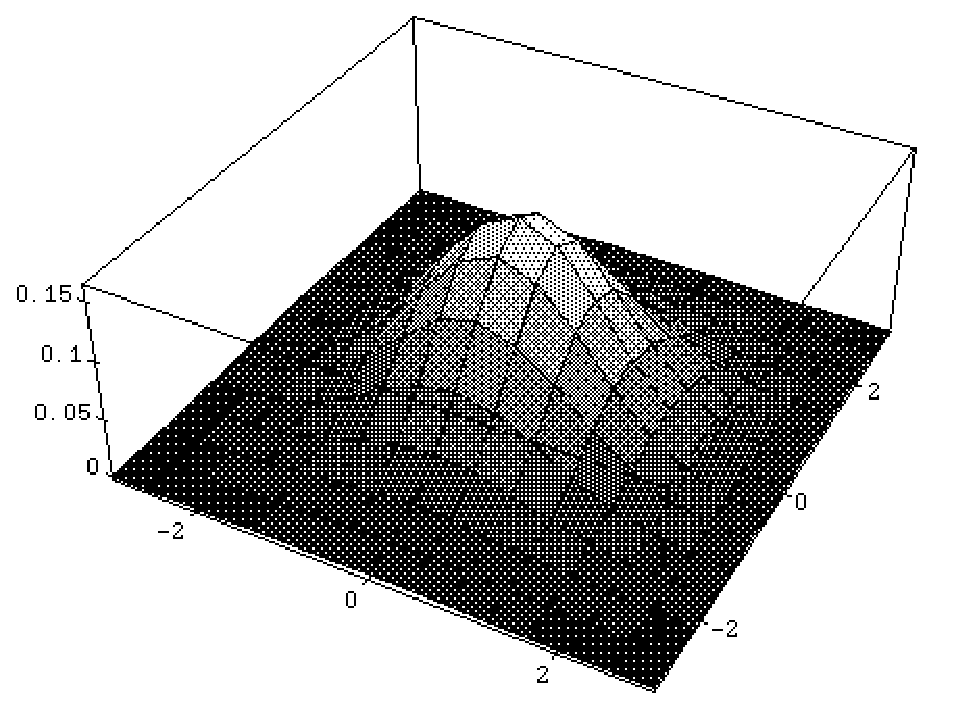
\includegraphics{normal2d.eps}\caption{Gráfica de la función de densidad normal
estándar}
\end{figure}



\begin{proposition}
 Si $X$ e $Y$ son conjuntamente gaussianas entonces:

\begin{enumerate}[a)]
\item $X+Y$ sigue una distribución normal de media $E(X+Y)=\mu_X+\mu_Y$ y varianza
$Var(X+Y)=\sigma_X^2+\sigma_Y^2+2 \sigma_{XY}$. De hecho cualquier combinación lineal no
trivial de $X$ e $Y$ es normal.
\item $Cov(X,Y)=0$ si y sólo si $X$ e $Y$ son independientes.
\item sus marginales son normales.
\end{enumerate}
\end{proposition}

\begin{proposition}
 Si $X$ es una v.a. normal e  $Y$ es otra variable normal y son independientes entonces
$X$ e $Y$ son conjuntamente normales.
\end{proposition}
\begin{proposition}
Sean $X$ e $Y$ dos v.a. conjuntamente normales entonces:

\begin{enumerate}[a)]
\item $X+Y$ sigue una distribución normal de media $E(X+Y)=\mu_X+mu_Y$ y varianza
$Var(X+Y)=\sigma_X^2+\sigma_Y^2+2 \sigma_{XY}$.
\item $Cov(x,y)=0$ si y sólo si $X$ e $Y$ son independientes.
\end{enumerate}
\end{proposition}
\subsection{La ley normal multivariante}

No la definimos aquí, es una generalización de la normal bidimensional y al igual que ella
su función de distribución queda definida por el vector de medias y la matriz de varianzas-covarianzas.

\begin{proposition}
\begin{enumerate}[a)]
\item Sean $X_1,X_2,\ldots,X_n$ $n$ v.a. que sigan una ley conjunta normal entonces cualquier
combinación lineal no trivial de $X_1,\ldots X_n$ sigue una ley normal unidimensional
\item Si $X_1,X_2,\ldots,X_n$ son v.a. normales univariantes e independientes entonces son
conjuntamente normales.
\item Como consecuencia de los resultados anteriores si $X_1,X_2,\ldots,X_n$
son v.a. normales univariantes e independientes entonces cualquier combinación lineal no
trivial de ellas es normal univariante.
\item Las marginales de una normal multivariante son normales.
\end{enumerate}
\end{proposition}

Estas propiedades nos serán de utilidad en la siguiente sección.

\section{Teorema  del Límite Central (T.L.C.)}

    Sean $X_{1},X_{2},\ldots,X_{n}$ v.a. independientes e idénticamente distribuidas (iid.)
    con $E(X_i)=\mu$ y $Var(X_i)=\sigma^2$ para $i=1,2,\ldots,n$.
    Sea $X=X_{1}+X_{2}+\ldots+X_{n}$
    entonces se tiene que:
    $E(X)=n\mu$ y $Var(x)= n\sigma^2$

    Además podemos ``tipificar'' $X$ de forma que :
    $$Z=\frac{X-E(X)}{\sqrt{Var(X)}}=\frac{X-n\mu}{\sqrt{n\sigma^2}}$$
    Operando obtenemos que $Z$ se puede poner como:
    $$Z=\frac{\overline{X}-\mu}{\frac{\sigma}{\sqrt{n}}}$$

    donde
    $$\overline{X}=\frac{X_{1}+X_{2}+\ldots+X_{n}}{n}=\frac{X}{n}$$


Se deja como ejercicio la demostración de las siguientes propiedades:

    \begin{proposition} Con las notaciones y condiciones anteriores:
\begin{enumerate}[a)]
\item $E(\sum_{i=1}^n X_i)=n \mu$ y $Var(\sum_{i=1}^n X_i)=n \sigma^2$.
\item $E(\overline{X})=\mu$ y $Var(\overline{X})=\frac{\sigma^2}{n}$.
\item $E(Z)=0$ y $Var(Z)=1$.
\end{enumerate}
\end{proposition}

 Notemos que si la distribución común a las variables es normal entonces
$Z$ es una combinación lineal de normales y por lo tanto conocemos su distribución. La
pregunta es ?`qué pasa cuando la distribución común no es normal sino otra cualquiera? La
respuesta nos la da el siguiente Teorema llamado del Límite Central.

    \subsubsection{Teorema del Límite Central }
    \begin{theorem}
Con las notaciones anteriores y cuando $n$ tiende a $\infty$ entonces

$$Z=\frac{X-n\mu}{\sqrt{n\sigma^2}}=\frac{\overline{X}-\mu}{\frac{\sigma}{\sqrt{n}}}$$
tiende a tener una distribución $N(0,1)$. Dicho de otra forma:


dado $x\in \R$ se tiene que

 $$\lim_{n\to\infty}P(Z\leq x)=\int_{-\infty}^x \frac{1}{\sqrt{2
\pi}} e^{-\frac{x^2}{2}}dx$$

\end{theorem}

Nota: La importancia de este teorema es tremenda pues nos dice que la distribución de
$\overline{X}$ en cualquier v.a. con cualquier distribución se aproxima, de alguna forma,
cuando $n$ crece a una distribución normal.

En particular podemos utilizar este resultado para aproximar las distribuciones que de
alguna manera sumen v.a. independientes con la misma distribución como es el caso de la
binomial y como es el espíritu de la Poisson. Pero tendremos un pequeño  problema que
estaremos aproximando una v.a. discreta por una continua, por lo que tendremos que realizar
pequeñas correcciones (se suelen llamar correcciones de continuidad de Fisher).

 \subsubsection{Aproximación de la distribución binomial y la Poisson
    por la normal}

    \textbf{Aproximación de una Binomial por una distribución normal}

    Veamos como utilizando el T.L.C. podemos aproximar por una
    distribución normal algunas distribuciones binomiales.

    Sea $X$ una v.a. con distribución $B(n,p)$ entonces $E(X)=np$
    y $Var(X)=npq$. También sabemos que $X=X_{1}+\cdots + X_{n}$ donde
    cada $X_{i}$ es una Bernouilli de parámetro $p$ e independientes
    entre si, entonces:

    $Z=\frac{X-E(X)}{\sqrt{Var(X)}}=\frac{X-np}{\sqrt{np(1-p)}}$

    Estamos en condiciones de aplicar el T.L.C.
%%%%%%%%La aproximación será buena si $n$ es grande
%%%%%%%% y $p$ no es muy cercano a $0$ ó $1$; también es buena si $n$ es pequeño
%%%%%%%% y p es cercana a $1/2$.
La aproximación se realiza de la siguiente manera:

$\bullet\  P(X=k)\approx P\left({{k-0.5-np}\over \sqrt{npq}}\leq Z \leq {{k+0.5-np}\over
\sqrt{npq}}\right)$


Mediante un razonamiento similar : $$\bullet\ P(X\leq k)\approx P\left(Z \leq
{{k+0.5-np}\over \sqrt{npq}}\right)$$ y

$\bullet\ P(a\leq X\leq b)\approx$

$\approx P\left(\frac{a-0.5-np}{\sqrt{npq}}\leq Z \leq \frac{b+0.5-np}{\sqrt{npq}}\right)$


Donde, en ambos casos $Z$ es la normal estándar.

%%%%%%%%
%%%%%%%%\textbf{Criterio:} La aproximación es fiables si $np(1-p)>9$ y $n\geq 20$ y $p$ próximo a
%%%%%%%%0.5

\textbf{Corrección de continuidad} El motivo de sumar o restar 0.5 en las aproximaciones es
corregir el efecto que tienen aproximar una v.a. discreta por una continua. Esta operación
recibe el nombre de corrección de continuidad de Fisher. Gráficamente el área que hacemos
corresponder a la probabilidad de cada valor entero $k$ en una binomial corresponde a la
comprendida entre la curva normal y el  segmento centrado en $k$ de amplitud 1.

\begin{example}
    $X$=número de caras en 100 lanzamientos de una moneda.
    $P(\mbox{cara})=\frac{1}{2}$. Calcular:

    \begin{enumerate}[a)]
    \item $P(40\leq X\leq 49)$
    \item $P(X=37)$
    \item $P(X\leq 50)$
    \end{enumerate}
    Solución:

    $E(X)=50=\mu_{X}$, $Var(X)=25$ y $\sigma_{X}=5$

    $Z=\frac{X-50}{5}$ por   el T.L.C. se  aproxima a  normal  estándar
    %%%%%%%%y tenemos que
%%%%%%%%    $n=1000$, $np(1-p)=25$ y $p=0.5$

    Entonces

    $P(40\leq X\leq 49)\approx P(\frac{40-0.5-50}{5}\leq Z\leq
    \frac{49+0.5-50}{5})=P(-\frac{10.5}{5}\leq Z\leq -\frac{0.5}{5})=
    F_{Z}(-\frac{0.5}{5})-  F_{Z}(-\frac{10.5}{5})=
    1-F_{Z}(\frac{0.5}{5})-1+F_{Z}(\frac{10.5}{5})=
F_{Z}(\frac{10.5}{5})-F_{Z}(\frac{0.5}{5})=F_{Z}(2.1)-F_{Z}(0.1)=0.9821-0.5398=0.4423$

La probabilidad exacta da $0.442605$. !!La aproximación es bastante buena!!

b) $P(X=37)=P(37\leq X\leq 37)\approx P(\frac{37-0.5-50}{5}\leq Z\leq
\frac{37+0.5-50}{5})=P(-\frac{13.5}{5}\leq Z\leq -\frac{12.5}{5})=
F_{Z}(\frac{13.5}{5})+F_{Z}(\frac{12.5}{5})=F_{Z}(2.7)-F_{Z}(2.5)= 0.9965-0.9938=0.0027$

La probabilidad exacta da $0.0026979$. !!La aproximación es bastante buena!!


c) $P(X\leq 50)\approx P(Z\leq \frac{50+0.5-50}{5})=P(Z\leq 0.5)=F_{Z}(0.1)=0.5398$

La probabilidad exacta calculada con un programa adecuado  da $0.539795$ !!La aproximación
es bastante buena!!

\end{example}


\textbf{Aproximación de una Poisson por una distribución normal}

De forma similar, y aplicando también la corrección de continuidad podemos aproximar la
probabilidad de una v.a. Poisson por una normal.

Si $X\equiv Po(\lambda)$ y $\lambda$ es grande, entonces podemos utilizar el TLC o también esta otra
aproximación:

$$\bullet\ P(X=k) \approx P\left({{k-0.5-\lambda} \over
\sqrt{\lambda}}\leq Z \leq {{k+0.5-\lambda}\over \sqrt{\lambda}}\right)$$


Mediante un razonamiento similar : $$\bullet\ P(X\leq k)\approx P\left(Z \leq
{{k+0.5-\lambda}\over \sqrt{\lambda}}\right)$$ y

$$\bullet\ P(a\leq X\leq b)\approx P\left(\frac{a-0.5-\lambda}{
\sqrt{\lambda}}\leq Z \leq \frac{b+0.5-\lambda}{ \sqrt{\lambda}}\right)$$

    \begin{example}
    Sea $X$=número de trabajos que llegan a un centro de cálculo en
    un lapso de $60$ minutos.

    Supongamos que $X$ siga una ley Poisson y que el número medio de
    trabajos que llegan por minuto sea $0.2$.
    Entonces $E(X)=0.2\cdot60=12$ por lo tanto $X$ es una $Po(12)$ es
    decir $\lambda =12$ y por lo tanto $\mu_X=12$ y $\sigma_X^2=12$.

    Si queremos calcular

    $P(Y\leq 10)\approx P(Z\leq \frac{10+0.5-12}{\sqrt{12}})=P(Z\leq -0.4330127)$

  $F_{Z}(-0.4330127)\approx 1-F_{Z}(0.43)=1-0.6664=0.3336$

La probabilidad exacta\footnote{Con R es  ppois(10,12) }  da $0.347229$. La aproximación es  buena.
\end{example}




% \texbf{Propiedades de la suma de normales y $\chi^{2}$}
%
% \begin{enumerate}[a)]
% \item Si $X_{1}\equiv N(\mu_{1},\sigma_{1}^{2})$ , $X_{2}\equiv
% N(\mu_{2},\sigma_{2}^{2})$  y son independientes entonces
% $$X_{1}+X_{2}\equiv N(\mu_{1}+\mu_{1},\sigma_{1}^{2}+\sigma_{2}^{2})$$
% \item Si $X_{1}\equiv \chi_{n_{1}}^{2}$ , $X_{2}\equiv
% \chi_{n_{2}}^{2}$  y son independientes entonces
% $$X=X_{1}+X_{2}\equiv \chi_{n_{1}+n_{2}}^{2}$$
% \end{enumerate}


    %%%
  %  \newline

\chapter{Muestreo Estadístico}
  
En esta tema sentaremos las bases del muestreo estadístico y estudiaremos las
distribuciones de algunos estadísticos muestrales; como la media aritmética, las proporciones y la varianza.

\section{Conceptos básicos}

  Aunque en el tema  dedicado a   la estadística descriptiva ya vimos
  algunos de los conceptos básicos sobre muestras, no está de más
  que los repasemos y ampliemos:

  \begin{description}

  \item \textbf{Población}: Conjunto de individuos con una característica observable
  común.

  \item \textbf{Muestra}: Subconjunto de la población del que se espera que la
  represente.
\end{description}

  El objetivo de la \textbf{estadística inferencial} es obtener
  información sobre el conjunto de la población a partir de un
  subconjunto representativo de ella llamado muestra.

  En la práctica lo más común es conocer sólo una parte de  la
  población y lo que queremos es averiguar por ejemplo qu\'e esperanza o
  qué varianza o \ldots\  tiene determinada población.
 \begin{description}
\item \textbf{Inferir información} de una muestra es contestar
  preguntas sobre
  el total de la población a partir del estudio de una muestra
  representativa de la misma.
\end{description}
  \subsubsection{Pasos en un estudio con muestreo}

  \begin{enumerate}[a)]
      \item ¿Qué información se necesita?
      \item ¿Cuál es la información relevante? ?`Se dispone de acceso
      a todos los individuos de la población?
      \item ¿Cómo seleccionamos los individuos de la muestra?
      \item ¿Qué método emplearemos para obtener la información de
      los individuos de la muestra?
      \item ¿Qué herramientas  utilizaremos para hacer inferencias?
      \item  ¿Qué conclusiones podemos obtener?
      \item   Si las conclusiones son fiables y suficientes
      redactar informe, en caso contrario  volver a empezar.
   \end{enumerate}


\subsection{Tipos de muestreo}


El objetivo de las técnica de muestreo es encontrar métodos para seleccionar muestras representativas de la población.

Las técnicas básicas son: el muestreo aleatorio simple, el muestreo aleatorio estratificado, el muestreo sistemático y el muestreo polietápico. Cada una de estas técnicas proporciona una muestra representativa de la población

\begin{itemize}
\item \textbf{Muestreo aleatorio probabilístico}
El muestreo aleatorio consiste en seleccionar muestra de la población con igual probabilidad. Esto quiere decir que cualquier conjunto de individuos tiene la misma probabilidad de ser seleccionado. 

Pensemos en una urna con $100$ bolas de colores. Hay dos maneras de obtener una muestra de $10$ bolas. Una podría ser sacar una bola de la urna, observar su color y devolverla a la urna. Es decir vamos obteniendo individuos y los volvemos a poner en la urna. Este tipo de muestreo recibe el nombre de \textbf{muestreo con reposición} o \textbf{muestreo aleatorio simple}. Otra forma sería repetir la experiencia anterior pero no devolver las bolas a la urna. En este caso también sucede que cualquier selección de los $10$ individuos es equiprobable. En este caso se habla de \textbf{muestreo aleatorio sin reemplazo}.


Notemos que el muestreo aleatorio con reemplazo o simple y el muestreo aleatorio sin reemplazo serán prácticamente el mismo  cuando el tamaño de la población sea muy grande en relación a la muestra y la probabilidad de que dos individuos se repitan sea muy pequeña. De todas maneras si la población es pequeña se suelen aplicar estadísticos corregidos por el efecto de población finita.

\item \textbf{Muestreo Aleatorio Estratificado}

En el caso en que la población  esté dividida en grupos o estratos  y que estos sean de interéas para la variable del estudio se toman muestras donde cada grupo esté representado en función de su tamaño. Por ejemplo los estratos podrían ser las grupos  de edad, o en las Islas Baleares por islas en proporción a  su número de habitantes,, en una provicia por municipios también en función de su número de habitantes, por estratos de nivel educativo .....


En estos casos Se determina el tamaño de la muestra en cada estrato y luego se toma una muestra aleatoria simple en ese bloque.


  
\item \textbf{ Muestreo por conglomerados}

El proceso de obtener una muestra aleatoria es caro. Por ejemplo  si el estudio se realiza por ejemplo sobre conjuntos de personas. Pesemos que queremos saber los hábitos de seguridad vial que tienen los estudiantes de primaria de Baleares. Para ello, previo permiso de la autoridad responsable queremos seleccionar una muestra representativa de los escolares de Baleares.  Lo lógico es que una vez los encuestadores estén en un centro pregunten a varios alumnos.
La selección de los colegios debe ser al azar.

Lo mismo para una encuesta  en una ciudad, seleccionaremos un edificio e intentaremos encuesta a todos sus habitantes. La selección de los bloques debe ser al azar.

% Muestreo Sistemático
% es de por listas no  lo ponenmos
%
\item \textbf{Muestreo Polietápico} 
En este caso se selecciona en etapas sucesivas grupos de la población. Por ejemplo encuesta a escolares de ESO de Mallorca, primero seleccionan al azar los centros y luego las clases y luego los individuos o se hace un muestreo por bloque de una clase.
\item \textbf{\item Muestreo no probabilístico}
Cuando nos tenemos que confomar con la información disponible o  la obtenida voluntariamente

\item  Combinaciones de las técnicas anteriores y otro tipos de técnicas dan lugar a nuevo tipos de muestreo estadístico.
\end{itemize}

En cada tipo de muestro se emplean técnicas  para estimar los resultados de interés: proporciones, medias , varianzas...

En cada uno de los tipos de muestreo las técnicas de estimación puede ser diferentes.

En este módulo sólo se estudian técnicas de estimación para el caso de  muestreo aleatorio simple.




\subsubsection{Muestreo aleatorio simple}


Estudiemos un poco más en detalle el caso del muestreo aleatorio simple con o sin reposición.
La idea es que queremos seleccionar una muestra de tamaño $n$ (es decir formada por $n$ individuos) 
de una población de tamaño $N$.
Obtendremos una muestra aleatoria simple  cuando todas las muestras posibles de $n$ individuos tengan la misma probabilidad de ser elegidas.

El tener una m.a.s de una población junto con un tamaño muestral adecuado nos asegurará la suficiente representatividad  de la muestra.

Hagamos algunas observaciones:

\begin{itemize}
      \item El proceso mismo del muestreo aleatorio simple es complejo.
      \item Una forma sencilla es numerar, si es posible a todos los
      individuos de la población y sortearlos eligiendo números como si se
      tratase de una lotería; por ejemplo con una tabla de números
      aleatorios\footnote{En realidad los números aleatorios generados por
      diversos tipos de algoritmos  son pseudoalatorios; son números que superan determinados
      test de aleatoriedad} o con un generador de números aleatorios; por ejemplo el que llevan nuestra hoja de cálculo.
      \item En ocasiones esto es impracticable o caro:
      \begin{enumerate}[a)]
          \item Población mundial de seres humanos.
          \item Población de llamadas a una centralita telefónica.
          \item Población de votantes en las próximas elecciones locales
          y autonómicas.
			\end{enumerate}

      \item En algunos de estos casos será luego impracticable localizar a
      los individuos seleccionados y convencerlos de que respondan, muchos no querrán.
\end{itemize}

\section{Inferencias}

       Nuestro interés es estudiar la distribución de probabilidad de la
       muestra o de alguna función de la muestra y de esta inferir
       resultados  de la distribución de probabilidad de la población.

\subsubsection{Estadísticos y distribuciones muestrales} 

Supongamos que tenemos
una muestra aleatoria simple de una población y deseamos obtener información sobre la media o la varianza
poblacionales. Estas inferencias las basaremos en un estadístico, que estudiaremos en más
profundidad en  los temas siguientes y  que no es más que una función que depende de la
muestra. p e: media aritmética, proporción muestral\ldots

\subsection{Distribución muestral de un estadístico}

La \textbf{distribución muestral  o distribución en el muestreo} de un estadístico es la
distribución de probabilidad de los valores que puede tomar el estadístico en todas las
posibles muestras, es decir la distribución de la variable aleatoria que define el
estadístico.

Veamos un ejemplo:

  \begin{example}
      Supongamos que queremos estimar cuál es número medio de
      municiones defectuosas una determinada marca por cada caja de 10 municiones cada una.
      Para ello tomamos una muestra aleatoria simple de cuatro cajas $X_{1}$, $X_{2}$
      $X_{3}$, $X_{4}$, las probamos y  obtenemos  los
      siguientes resultados:


      \begin{tabular}{lccl}
     primera caja &: & 1 &defectuoso\\
     segunda caja &: & 2 &defectuosos\\
     tercera caja &: & 0 &defectuoso\\
     cuarta  caja &: & 1 &defectuosos
     \end{tabular}

     Definimos el estadístico media aritmética de munición defectuosa como:

     $$\overline{X}=T(X_{1}, X_{2}, X_{3},
     X_{4})=\frac{X_{1}+X_{2}+X_{3}+X_{4}}{4}$$

     En este caso $\overline{X}=1$.
\end{example}

   Supongamos que tomamos repetidas muestras de tamaño 4 y los
     resultados son:
\begin{center}

     \begin{tabular}{c|c|c|c|c|c|c|c|c|c}
      M. & M. & M. & M. & M. & M. & M. & M. & M. & M.\\
1 & 2 & 3 & 4 & 5 & 6 & 7 & 8 & 9 & 10 \\ \hline 0&1&3&0&0&1&0&0&0&1\\
1&1&1&0&1&1&1&0&0&2\\ 0&1&2&1&0&0&1&2&0&1\\ 1&1&2&2&1&3&0&0&1&1
\end{tabular}
\end{center}

\begin{center}
     \begin{tabular}{c|c|c|c|c|c|c|c|c|c}
     M. & M. & M. & M. & M. & M. & M. & M. & M. & M.\\
11 & 12 & 13 & 14 & 15 & 16 & 17 & 18 &  19 & 20 \\
 \hline
0&0&1&2&0&2&1&2&1&1\\ 1&0&1&0&1&1&2&0&0&1\\ 1&0&2&0&1&1&0&1&1&0\\ 3&3&1&0&0&2&1&0&1&1
\end{tabular}
\end{center}



Las medias aritméticas de cada muestra son:

\begin{center}

\begin{tabular}{ccccc}
 0.50&1.00&2.00&0.75&0.50\\
 1.25&0.50&0.50&0.25&1.25\\
 1.25&0.75&1.25&0.50&0.50\\
 1.50&1.00&0.75&0.75&0.75
  \end{tabular}
  \end{center}
  %\end{example}

  Entonces:
  $$P_{\overline{X}}(0.25))=P(\overline{X}=0.25)=\frac{1}{20}=0.05$$
  $$P_{\overline{X}}(0.50))=P(\overline{X}=0.50)=\frac{6}{20}=0.30$$
  $$P_{\overline{X}}(0.75))=P(\overline{X}=0.75)=\frac{5}{20}=0.25$$
  $$P_{\overline{X}}(1))=P(\overline{X}=1)=\frac{2}{2}=0.10$$
  $$P_{\overline{X}}(1.25))=P(\overline{X}=1.25)=\frac{4}{20}=0.20$$
  $$P_{\overline{X}}(1.50))=P(\overline{X}=1.5)=\frac{1}{20}=0.05$$
  $$P_{\overline{X}}(2))=P(\overline{X}=2)=\frac{1}{20}=0.05$$

   Esta sería una aproximación a la distribución muestral del
   estadístico $\overline{X}$ a partir de los datos de varias
   muestras.


 \subsection{Distribución  la media muestral}
 La distribución del estadístico puede seguir un modelo preestablecido si se cumplen varias condiciones. Por ejemplo,
 supongamos que hemos tomado una muestra aleatoria simple de $n$ observaciones
 de una v.a. $X$ en una población de media $\mu_{X}$ y desviación típica $\sigma_{X}$.

 Representemos por $X_{1}, X_{2},\ldots,X_{n}$ los elementos de
 $n$ observaciones independientes que forman
 una muestra aleatoria simple de ésta población. Cada una de las observaciones de
 la población son así mismo variables aleatorias con la misma esperanza y varianza que
 la población.

 Llamaremos \textbf{media aritmética o media muestral}  de la muestra
 $X_{1},\ldots,X_{n}$ a
 
 $$\overline{X}=\frac{\sum_{i=1}^n X_{i}}{n}$$

 %\textbf{Observaciones:}
 
 Resaltemos que:

\begin{enumerate}[a)]
\item $E(\overline{X})=\frac{1}{n}E(X_{1}+X_{2}+\cdots
+X_{n})=\frac{1}{n}
 (\mu_{X}+\mu_{X}+\cdots+\mu_{X})=\mu_{X}$
 \item El valor esperando de la media aritmética de la muestra es la media
 poblacional. Entonces el estadístico media muestral \textit{estima}
 la media poblacional. Dicho de otra forma la esperanza de la
 distribución muestral de la media aritmética es la media poblacional.
\end{enumerate}



 Pero que el valor esperado sea $\mu_{X}$ no quiere decir que
 $\overline{X}$ sea exactamente $\mu_{X}$. Estudiemos la varianza de
 $\overline{X}$. Como  $X_{1},\ldots,X_{n}$ son independientes tenemos
 que:

\begin {enumerate}[a)]
\item $Var(\overline{X})=\frac{1}{n^2}Var(X_{1}+X_{2}+\cdots +X_{n})=
\frac{1}{n^2}(Var(X_{1})+Var(X_{2})+\cdots +Var(X_{n}))= \frac{1}{n^2}
n\sigma_{X}^2=\frac{1}{n} \sigma_{X}^2$
\item  Luego  si $n$ es suficientemente grande ( o cuando $n\to\infty$) la
 varianza tenderá a estar muy próxima a cero.
\end{enumerate}

\begin{example}
No siempre tendremos independencia entre $X_{1},\ldots,X_{n}$.
 Por ejemplo  supongamos que queremos averiguar cuántos votos
 afirmativos hay en una urna con $10$ votos. Tenemos dos opciones para
 realizar la muestra aleatoria simple:

 \begin{enumerate}[a)]
 \item Tomar un voto al azar anotar su resultado y devolverlo a la urna,
 repetir el proceso $3$ veces más. En este caso es un muestreo con reemplazamiento.
 \item Tomar sucesivamente $4$ votos de la urna sin reemplazarlos.
 En este caso es un muestreo reemplazamiento.
 \end{enumerate}

 En ambos casos la muestra obtenida es una muestra aleatoria  pues todos los
 subconjuntos de individuos tienen igual probabilidad de ser elegidos.

 Pero en el primer caso tenemos independencia entre cada una de las
 observaciones mientras que en el segundo esto no es así.
\end{example}

 En la práctica se elige casi siempre el muestreo consistente en
 observar n individuos distintos. Además si  $n$ es pequeño con respecto al tamaño de la población $N$
 podemos suponer que las variables son prácticamente independientes.
 Si no, tenemos que corregir la varianza multiplicándola por lo que se
 llama \textbf{factor de población finita} y tendremos que

 $$\sigma_{\overline{X}}^2=Var(\overline{X})=\frac{1}{n} \sigma_{X}^2 \frac{N-n}{N-1}$$


 Frecuentemente utilizaremos la expresión tipificada de la media muestral:

 $$Z=\frac{\overline{X}-\mu_{\overline{X}}}{\sigma_{\overline{X}}}
 =\frac{\overline{X}-\mu_{X}}{\frac{\sigma_{X}}{\sqrt{n}}}$$

 Además para  tamaños muestrales grandes aplicando  el Teorema del Límite Central  la
 distribución de $Z$ es una normal estándar. Este resultado es muy importante
 pues \textbf{sea cual sea la distribución de $X$ la distribución de
  $\overline{X}$ será conocida si $n$ es suficientemente grande}.


\subsubsection{Distribución muestral de $\overline{X}$}
 Sea $X$ la variable aleatoria de interés que queremos observar en  una cierta población. Supongamos que 
 la esperanza pobalacional es  $E(X)=\mu_{X}$ y su  varianza $Var(X)=\sigma_{X}^2$. Sea
$X_{1},\ldots, X_{n}$ una muestra aleatoria simple de dicha población:


Entonces se cumplen las propiedades siguientes:

\begin{enumerate}[a)]
\item $\mu_{\overline{X}}=E(\overline{X})=\mu_{X}$; el valor esperado de la media es la media poblacional.
\item La varianza y la desviación típica de $\overline{X}$ se pueden obtener con las siguientes fórmulas $\sigma_{\overline{X}}^2=\frac{1}{n}\sigma_{X}^2$
 y  la desviación típica de $\overline{X}$ es $\sigma_{\overline{X}}=
 \frac{\sigma_{X}}{\sqrt{n}}$
 que también recibe el nombre de error estándar de $\overline{X}$.

\item En el caso en que el tamaño muestral $n$ no sea
\emph{pequeño} en relación al tamaño de la población  entonces
  tenemos que aplicar el factor de corrección de población finita en
  el cálculo del error estándar de $\overline{X}$:

 $$\sigma_{\overline{X}}^2=\frac{1}{n}\sigma_{X}^2\frac{N-n}{N-1}$$
 y  el error estándar será
 $\sigma_{\overline{X}}=\frac{\sigma_{X}}{\sqrt{n}}\sqrt{\frac{N-n}{N-1}}$
 \item Si la distribución de la población ($X$) es normal entonces
 la variable aleatoria:
 $$Z=\frac{\overline{X}-\mu_{X}}{\frac{\sigma_{X}}{\sqrt{n}}}$$

 es una normal estándar. O lo que es lo mismo $\overline{X}$ es una
 normal con media $\mu_{X}$ y  desviación típica
 $\sigma_{\overline{X}}$
 \item Si la distribución de la población no es normal pero el tamaño
 muestral es suficientemente grande entones por el T.L.C.
 la distribución de $Z$ también se aproxima a una normal estándar y
 por lo tanto $\overline{X}$ se aproxima a una
 normal con media $\mu_{X}$ y  desviación típica
 $\sigma_{\overline{X}}$
\end{enumerate}


 \begin{example}
    El precio medio por $m^2$ de venta de casas nuevas durante el último año
    en una determinada ciudad  fue de 115000 pts. La desviación
    típica de la población fue de 25000 pts. Se toma una muestra
    aleatoria de 100 casas nuevas de esta ciudad.
    \begin{enumerate}[a)]
        \item ¿Cuál es la probabilidad de que la media muestral de los
        precios de venta sea menor que 110000 pts?
        \item ¿Cuál es la probabilidad de que la media muestral de los
        precios de venta esté entre 113000 pts y 117000 pts?
        \item¿Cuál es la probabilidad de que la media muestral de los
        precios de venta esté entre 114000 pts y 116000 pts?
        \item Sin hacer cálculos, razonar en cuál de los siguientes rangos
        resulta más probable que se encuentre la media muestral de los
        precios de venta:
        \begin{center}
        \begin{tabular}{ll}
        113000 pts.-&115000 pts.\\
        114000 pts.-&116000 pts.\\
        115000 pts.-&117000 pts.\\
        116000 pts.-&118000 pts.
            \end{tabular}
            \end{center}
        \end{enumerate}
 \end{example}

Supongamos que el número de casas de la ciudad sea  muy grande en relación al tamaño
muestral $n=100$. Entones si $X$ es  la v.a. precio de una casa de la ciudad el enunciado
nos dice que $\mu_{X}=E(X)=115000$. y $\sigma_{X}=25000$. Tomamos una muestra aleatoria simple
$X_{1},\ldots,X_{100}$ de precios entonces F $\mu_{\overline{X}}=\mu_{X}=115000$ y
$\sigma_{\overline{X}}= \frac{\sigma_{X}}{\sqrt{n}}=\frac{25000}{\sqrt{100}}=2500$

Además $Z=\frac{\overline{X}-\mu_{X}}{\frac{\sigma_{X}}{\sqrt{n}}}=
\frac{\overline{X}-115000}{2500}$
 sigue aproximadamente una distribución normal estándar.

     \textbf{Solución:}

 a) $P(\overline{X}\leq 110000)=\\ P(Z\leq \frac{110000-115000}{2500})=$
 $P(Z\leq -2)=F_{Z}(-2)=1-F_{Z}(2)=1-0.9772=0.0228$

  b) $P(113000\leq  \overline{X} \leq 117000)=\\ P(\frac{113000-115000}{2500}\leq
  Z \leq \frac{117000-115000}{2500})=$
  $F_{Z}(0.8)-F_{Z}(-0.8)=
  2 F_{Z}(0.8) -1= 2 (0.7881)-1=0.5762$

  c) $P(114000\leq  \overline{X} \leq 116000)=\\ P(\frac{114000-115000}{2500}\leq
  Z \leq \frac{116000-115000}{2500})=$
  $F_{Z}(0.4)-F_{Z}(-0.4)=2 F_{Z}(0.8) -1= 2 (0.6554)-1=0.3108$

  d) La media aritmética de los precios $\overline{X}$ sigue
  aproximadamente una distribución normal entonces gráficamente el
  intervalo de mayor probabilidad será el que mayor área cubra bajo
  la curva normal (centrada en 115000) y ese intervalo es
  114000 pts.-116000 pts.


    \subsection{Distribución de una proporción muestral}
    La proporción muestral de un evento en una población vendrá
    generalmente asociada a una variable binomial (si la población es
    pequeña será Hipergeométrica).

    Por ejemplo si tomamos una muestra de tamaño $n$, determinar
    el porcentaje de votos que recibirá el Partido P.X. en las
    próximas elecciones es lo mismo que determinar el parámetro $p$ de
    $X=\sum_{i}^{n}X_i$ número de votantes de P.X. en la muestra de tamaño $n$,
    que es $B(n,p)$ y donde cada $X_i$ es una $Ber(p)$ independiente de forma que $X_i=1$
    si el iésimo individuo y cero en caso contrario, así que la proporción muetral es la media
    aritmética de observaciones $Ber(p)$.

    ¿Será realmente binomial? Notemos que en la
    muestra no preguntaremos dos veces al mismo individuo,
    luego las observaciones no son exactamente independientes,
    pero si el tamaño de la población es grande respecto a
    la muestra podemos considerarlas así, ya que la probabilidad de repuesta afirmativa no cambia
    (es despreciable el cambio).

    \begin{definition}
    Sea $X$ el número de éxitos en una muestra binomial de $n$
    observaciones, con probabilidad de éxito $p$. Entonces la
    proporción de éxitos en la muestra es:

    $\hat{p}_{X}=\frac{X}{n}$,  y se denomina proporción muestral.
\end{definition}

    \subsubsection{Distribución en el muestreo de   $\mathbf{\hat{p}_{X}}$}

    Sea   $\hat{p}_{X}$ la proporción de éxitos en una muestra
    aleatoria de $n$ observaciones. Entonces:

    \begin{enumerate}[a)]
    \item  $E(\hat{p}_{X})=E(\frac{X}{n})=\frac{E(X)}{n}=\frac{np}{n}=p$
    \item  La distribución muestral de $\hat{p}_{X}$  tiene
    varianza $\sigma_{\hat{p}_{X}}^2=Var(\frac{X}{n})=\frac{Var(X)}{n^2}
    =\frac{np(1-p)}{n^2}=\frac{p(1-p)}{n}$ y por lo tanto su desviación
    típica es
    $\sigma_{\hat{p}_{X} }=\sqrt{\frac{p(1-p)}{n}}$

    que recibe también el nombre de error estándar de la proporción
    muestral
    \item Si $n$ es pequeño en relación al tamaño de la población $N$
    tenemos que aplicar el factor de corrección de población finita
  y entonces el error estándar de  $\hat{p}_{X}$  es

    $$\sigma_{\hat{p}_{X} }=\sqrt{\frac{p(1-p)}{n}}
  \sqrt{\frac{N-n}{N-1}}.$$
  \item Si el tamaño muestral es grande (por ejemplo $n>30$ o mejor  $n>40$) entonces

  $$Z=\frac{\hat{p}_{X}- p}{\sigma_{\hat{p}_{X}}},$$

  y que se distribuye aproximadamente como una normal estándar
  o lo que es lo mismo $\hat{p}_{X}$ se distribuye aproximadamente
  como una normal con esperanza $p_{X}$ y varianza
  $\sigma_{\hat{p}_{X}}$.

  \item Cuando no se verifiquen las condiciones de aproximación
  utilizaremos la distribución $t$ de Student que veremos el el siguiente tema.
\end{enumerate}

 \textbf{Observación} Notemos que si $n$ crece el error estándar
    disminuye y entonces $\hat{p}$ estará más cerca del valor real $p$.

     \begin{example}

        El dueño de una tienda de discos ha comprobado que el 20\% de los
    clientes que entran en su tienda realizan una compra. Cierta mañana
    entraron en esa tienda 180 personas, que pueden ser consideradas como
    una muestra aleatoria de todos sus clientes.
        \begin{enumerate}[a)]
        \item ¿Cuál será la media de la proporción muestral de clientes
        que realizaron alguna compra?
        \item ¿Cuál es la varianza de la proporción muestral?
        \item ¿Cuál es el error estándar de la proporción muestral?
        \item ¿Cuál es la probabilidad de que la proporción muestral sea
        mayor que 0.15?
        \end{enumerate}


   \textbf{Solución:}
    El tamaño de la muestra es pequeño en relación al
    número total de clientes. Tenemos que $p=0.2$ (probabilidad
    de éxito en la venta). Sea $X$= número de
    clientes que compran entre los 180, entonces:
\begin{enumerate}[a)]
  \item $E(\hat{p}_{X})=p=0.2$

  \item $\sigma_{\hat{p}_{X}}^2= \frac{ p(1-p)}{n}=\frac{0.2
    (1-0.2)}{180}=0.0009$

  \item $\sigma_{\hat{p}_{X}}=\sqrt{\frac{ p(1-p)}{n}}=\sqrt{0.0009}=0.03$
    \item Como $n$  es grande entonces
    $Z=\frac{\hat{p}_{X}-p}{\sigma_{\hat{p}_{X}}}=\frac{\hat{p}_{X}-0.2}{0.03}$
 sigue aproximadamente una distribución normal estándar, entonces:

 $P(\hat{p}_{X}>0.15)=1-P(\hat{p}_{X}\leq 0.15)= 1-P(Z\leq
 \frac{0.15-0.2}{0.03})=1-F_{Z}( -1.67)=F_{Z}(1.67)=0.9525$
\end{enumerate}
 \end{example}

    \subsection{Distribución muestral de la varianza muestral}

\begin{definition}
Sea $X_{1},\ldots, X_{n}$ una muestra aleatoria simple de una población ($X$) con
$E(X)=\mu_{X}$ y $Var(X)=\sigma_{X}^2$. Llamaremos
\underline{ \emph{varianza muestral}} a :

$\tilde{S}_{X}^2=\frac{\sum_{i=1}^n (X_{i}-\overline{X})^2}{n-1}$

$\tilde{S}_{X}=+\sqrt{S_{X}^2}$ recibe el nombre de desviación típica muestral.

Denotaremos por $S^2_{X}=\frac{n-1}{n}\tilde{S}^2_{X}$ y $S_X=+\sqrt{S_X^2}$.

\end{definition}

  \begin{proposition}
  \begin{enumerate}
\item $S^2_X=\frac{\sum_{i=1}^n (X_{i}-\overline{X})^2}{n}=\left(\frac{\sum_{i=1}^n
X_{i}^2}{n}-\overline{X}^2\right)$
\item $E(S^2_X)=\frac{n-1}{n} \sigma^2_X$
\item $\tilde{S}_{X}^2=\frac{n}{n-1}\left(\frac{\sum_{i=1}^n
X_{i}^2}{n}-\overline{X}^2\right)$
\item $E(\tilde{S}_{X}^2)=\sigma_{X}^2$
\end{enumerate}
\end{proposition}

    \subsubsection{Distribución en el muestreo de $\tilde{S}_{X}^2$}
    Con las notaciones anteriores tenemos que:

    \begin{enumerate}[a)]
        \item $E(\tilde{S}_{X}^2)=\sigma_{X}^2$
      %%%%%%%%  \item Si la distribución de la población es normal entonces:
%%%%%%%%        $Var(\rilde{S}_{X}^2)=\frac{2\sigma_{X}^2}{n-1}$
        \item Si la distribución de la población es normal entonces
        la variable $\frac{(n-1)\tilde{S}_{X}^2}{\sigma_{X}^2}$ se distribuye
        según una ley $\chi_{n-1}^2$
        \end{enumerate}

    \subsubsection{La distribución $\chi^{2}_{n}$ (chi-cuadrado con n g.l.)}

Si $X_{1},X_{2},\ldots, X_{n}$ son n  v.a. independientes y $X_{i}\equiv N(0,1)$ entonces:
$$X=X_{1}^{2}+X_{2}^{2}+\ldots +X_{n}^{2}$$ es una v.a. que diremos que se distribuye
chi-cuadrado con n grados de libertad y lo notaremos por $\chi^{2}_{n}$


La función de densidad de una $\chi^{2}_{n}$  es :
$$f(x)={\frac{1}{2^{n/2} \Gamma (n/2)}} x^{(n/2)-1} e^{-x/2}$$

con $x\geq 0$ y $\Gamma(n/2)=\int_{0}^{+\infty} u^{(n/2)-1}e^{-u}du$ la llamada función
gamma.

\begin{figure}

\begin{center}
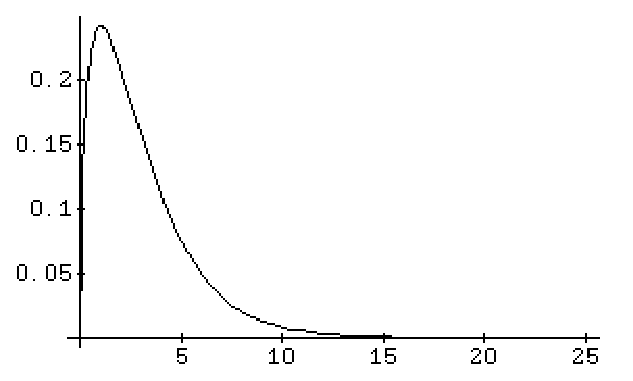
\includegraphics[scale=0.6]{chi2.eps}
\end{center}
\caption{Gráfica de la función de densidad de una $\chi^2$}
\end{figure}


%%\def\dibuixa{\scaledpicture 99.4mm by 61.3mm (c scaled 500)}

%%\dibuixa
Su función de distribución se puede calcular pero para nuestra comodidad está tabulada.


    \begin{example}

     Las rentabilidades mensuales de cierto tipo de
        acciones son independientes unas de otras, y siguen una
        distribución normal con desviación típica 1.7. Se toma una
        muestra de 12 meses.
        \begin{enumerate}[a)]
            \item Hallar la probabilidad de que la desviación típica muestral
            sea menor que 2.5.
            \item Hallar la probabilidad de que la desviación típica
            muestral sea mayor que 1.
            \end{enumerate}
            \end{example}


    \textbf{Solución}
Sea $X$= rentabilidad de las acciones. Sabemos que $\sigma_{X}^2=(1.7)^2$ además como la
distribución de la población es normal y $n=12$  tenemos que
$\frac{(n-1)\tilde{S}_{X}^2}{\sigma_{X}^2}$ sigue  una distribución $\chi^2_{11}$.

a) $P(\tilde{S}_{X}<2.5)=
P(\tilde{S}_{X}^2<(2.5)^2)=P(\frac{(12-1)\tilde{S}_{X}^2}{(1.7)^2}<\frac{(12-1)
(2.5)^2}{(1.7)^2})= P(\chi_{11}^2<23.7889)\approx P(\chi_{11}^2<24.725)=0.99.$

b)
$P(\tilde{S}_{X}>1)=P(\tilde{S}_{X}^2>1)=P(\frac{(12-1)\tilde{S}_{X}^2}{1.7^2}>\frac{(12-1)
1}{1.7^2})=P(\chi_{11}^2>3.80623)=\approx 1-P(\chi_{11}^2<3.816)=1-0.025=0.975$




%     \newline
%   \textbf{La distribuci\'on t de Student}
%
% Es aquella  que tiene por funci\'on de densidad:
% $$f(x)={{\Gamma \left({{n+1}\over 2}\right)}\over
% {\Gamma \left({{n}\over 2}\right)\sqrt{n
% \pi}}}\left(1+{{x^2}\over{n}}^{-(n+1)/2}\right)\mbox{ con }
% -\infty<x<\infty$$
%
%
% Se parece  a una normal.
%
%  A $t_{n}$ se le denomina $t$ de student con n grados de libertad.
% Gr\'aficas comparativas
% \dibu{t.epsf}{Gr\'afica de la funci\'on de densidad de una student
% }{densidadt}
%
%   \newline








  \chapter{ Inferencia estad\'{\i}stica: estimaci\'on de par\'ametros.}

  \section{Introducci\'on}

  En este tema estudiaremos como aproximar distintos par\'ametros
  poblacionales a partir de una m.a.s.
  formada por observaciones independientes de una  poblaci\'on, en los que sigue cuando digamos m.a.s. entenderemos
  que es una muestra aleatoria formada por observaciones independientes.

  Normalmente el par\'ametro (por ejemplo $\mu$, $\sigma$\ldots)
     tendr\'a distribuci\'on conocida o la aproximaremos por el T.L.C.

\section{Estimadores}

  \begin{definition}\textbf{Estad\'{\i}stico}: Sean $X_1,\ldots,X_n$ $n$ v.a. iid que forman una m.a.s.
  de una poblaci\'on. Un estad\'{\i}stico es una funci\'on de una de una
  muestra.
  \end{definition}
   Podemos decir que un estad\'{\i}stico una variable
  aleatoria que es funci\'on de la muestra.

  \begin{definition}\textbf{Estimador puntual}:
 Un \emph{estimador puntual} de un par\'ametro $\theta$ es un estad\'{\i}stico que da
 como resultado un \'unico valor del que se espera que se aproxime a $\theta$.

 Una \emph{realizaci\'on del estimador} $T(x_{1},\ldots,x_{n})=\hat{\theta }$
 en una muestra se llama \emph{ estimaci\'on puntual de par\'ametro}.
 \end{definition}


     \begin{example}  Dada una m.a.s.
     $X_{1},\ldots,X_{n}$ y una realizaci\'on de la misma
     $x_{1},\ldots,x_{n}$ los principales estimadores de los
     par\'ametros poblacionales que hemos visto son:

     \begin{center}

     \begin{tabular}{lll}
     \hline
     Par\'ametro & & \\
    Poblacional & Estimador($\theta$) & Estimaci\'on($\hat{\theta}$)\\
    &  &  \\
     \hline
    $\mu_{X}$ & $\overline{X}=\frac{\sum_{i=1}^n X_{i}}{n}$ &  $\overline{x}=\frac{\sum_{i=1}^n x_{i}}{n}$ \\
    %%$ \sigma_{X}^2$ & $S_{X}^2=\frac{\sum_{i=1}^n
%%    (X_{i}-\overline{X})^2}{n}$  & $s_{X}^2=\frac{\sum_{i=1}^n
%%    (X_{i}-\overline{X})^2}{n}$\\
%%    \hline
    $\sigma_{X}$ & $\tilde{S}_{X}=\frac{\sum_{i=1}^n
    (X_{i}-\overline{X})^2}{n-1}$ &
    $\tilde{s}_{X}=\frac{\sum_{i=1}^n
    (x_{i}-\overline{x})^2}{n-1}$\\\hline
    $p$ & $\hat{p}_{X}=\frac{\sum_{1}^n X_i}{n}$ & $\frac{\sum_{1}^n x_i}{n}$ \\
    \hline
    \end{tabular}
    \end{center}
     \end{example}

     \begin{example} Consideremos una m.a.s.
     $X_{1},X_{2},X_{3},X_{4},X_{5}$ del lanzamiento de un dado ($n=5$).

     Una realizaci\'on de esta muestra es
     $x_{1}=2,x_{2}=3,x_{3}=3,x_{4}=5,x_{5}=6$.


     Sabemos que, si el dado es perfecto, $\mu=3.5$;
     el estad\'{\i}stico de esta muestra es


    $$\overline{X}=\frac{X_{1}+X_{2}+X_{3}+X_{4}+X_{5}}{5}$$

     y una estimaci\'on es

    $$\overline{x}=\frac{x_{1}+x_{2}+x_{3}+x_{4}+x_{5}}{5}=
     \frac{2+3+3+5+6}{5}=\frac{19}{5}=3.8$$

    Si queremos estimar  la proporci\'on de veces que sale 3 es $p_{3}=
     \frac{1}{6}$

     el estad\'{\i}stico es
     $$\hat{p}_{3}=\frac{\mbox{frec. de 3 en la muestra}}{5}$$
     y una realizaci\'on ser\'a $\frac{2}{5}$.

         \end{example}

     \subsection{Estimadores insesgados}

     Vamos a ver en esta secci\'on algunas propiedades de los estimadores.
     La m\'as inmediata es pedirles que a medida que se aumente el tama\~{n}o
     muestral se aproximen m\'as al verdadero valor del par\'ametro.

     \begin{definition} \textbf{Estimador insesgado}
     Sea $\hat{\theta}$ un estimador de un par\'ametro poblacional
     $\theta$. Diremos que $\hat{\theta}$ es insesgado si
     $E(\hat{\theta})=\theta$.
     \end{definition}

     Es este caso la estimaci\'on puntual se dice que es insesgada.
     \begin{example}
         En el ejemplo anterior para cualquier muestra de tama\~{n}o
         $n$,  $X_{1},\ldots,X_{n}$, tenemos que
         $E(\overline{X})=\mu_{X}$ por lo tanto $\overline{X}$ es un estimador
         insesgado de $\mu_{X}$.
     \end{example}


\begin{proposition}
Dada una m.a.s. La media, varianza y proporci\'on muestrales son estimadores insesgados de
sus correspondientes par\'ametros poblacionales.
\end{proposition}

\begin{definition}\textbf{Sesgo}: Sea $\hat{\theta}$ un estimador puntual de un par\'ametro
poblacional $\theta$, llamaremos sesgo de $\hat{\theta}$ a:

$$Sesgo(\hat{\theta})=E(\hat{\theta})-\theta$$
\end{definition}

\textbf{Observaci\'on} Evidentemente un estimador es insesgado si y s\'olo si tiene sesgo cero.


    Una propiedad buena para un estimador es
    la  carencia de sesgo. Pero podr\'{\i}a suceder que tuviera una gran
    variabilidad, entonces aunque su valor central sea el verdadero valor del par\'ametro
    que se estima una realizaci\'on del  estad\'{\i}stico  podr\'{\i}a estar lejos del
    verdadero valor del par\'ametro. Parece pues interesante emplear aquellos estimadores
    que tengan varianza m\'as peque\~{n}a.


\begin{definition}\textbf{Eficiencia}:
Sean $\hat{\theta}_{1}$ y $\hat{\theta}_{2}$ dos estimadores de un par\'ametro poblacional
$\theta$ obtenidos de la misma muestra.

\begin{enumerate}[a)]
    \item Diremos que $\hat{\theta}_{1}$ es m\'as eficiente que $\hat{\theta}_{2}$
    si $Var(\hat{\theta}_{1})< Var(\hat{\theta}_{2})$
    \item Definimos la eficiencia relativa de $\hat{\theta}_{2}$
    respecto de
    $\hat{\theta}_{1}$ como

    $Eff.rel=\frac{Var(\hat{\theta}_{2})}{Var(\hat{\theta}_{1})}$


    de forma que si $Eff.rel<1$ entonces
    $\hat{\theta}_{1}$ es m\'as eficiente que $\hat{\theta}_{2}$

    \end{enumerate}
\end{definition}
    \begin{example}

    Sea $x_{1},\ldots,x_{n}$ la realizaci\'on ordenada de menor a mayor
     de una muestra de tama\~{n}o $n$. Se define la mediana muestral como

     $Me=\left\{\begin{array}{ll}
     x_{\frac{n+1}{2}} & \mbox{ si  } n  \mbox{  es impar }\\
      \frac{x_{\frac{n}{2}}+ x_{\frac{n}{2}+1}}{2} & \mbox{ si } n  \mbox{
      es par }\\
     \end{array}\right.$

     Como vimos en problemas la mediana es tambi\'en un valor de
     tendencia central, pero ?`es un buen estimador de $\mu$?

     Se puede demostrar que  si la poblaci\'on tiene distribuci\'on normal
     con media $\mu$ y varianza $\sigma_{X}^2$ entonces
     $E(Me)=\mu$ y $Var(Me)=\frac{\pi}{2}
     \frac{\sigma_{X}^2}{n}\approx \frac{1.57 \sigma_{X}^2}{n}$

      entonces
      $Eff. rel=\frac{Var(Me)}{Var(\overline{x})}=1.57$

      Luego si la muestra es de una poblaci\'on normal $\overline{X}$
      es m\'as eficiente  (un 57\% m\'as de varianza) que la Mediana.
      \end{example}

  \begin{definition}\textbf{Estimador m\'as eficiente}:

      Diremos que un estimador insesgado $\hat{\theta}$
      del pa\-r\'a\-me\-tro $\theta$ es el estimador m\'as eficiente si no
      existe ning\'un otro estimador insesgado que tenga menor varianza
      que \'el (tambi\'en se le denomina estimador insesgado de varianza
      m\'{\i}nima).

\end{definition}
      \begin{example}\footnote{ M\'as concretamente estos estimadores son del tipo UMVUE del
      acr\'onimo ingl\'es ``Uniformly Minimum Variance Unbiased Estimator": Estimadores
      insesgados uniformemente de m\'{\i}nima varianza".}
      \begin{itemize}
       \item Si la poblaci\'on es normal la media muestral es el
       estimador insesgado m\'as eficiente de la media poblacional.
       \item Si la poblaci\'on es normal la varianza muestral es el
       estimador insesgado  m\'as eficiente de la varianza poblacional.
       \item Si la poblaci\'on es binomial la proporci\'on muestral es el
       estimador insesgado m\'as eficiente de la proporci\'on poblacional.
      \end{itemize}
      \end{example}

\section{M\'etodos para calcular estimadores}

Existen diversos m\'etodos para el c\'alculo de estimadores:

\begin{itemize}
\item M\'etodo de los momentos. Momento central de orden $r$

$m_{r}=\frac{\sum_{i=1}^{n} (X_{i}-\overline{X})^r}{n}$

\item El de menor error cuadr\'atico medio

$E((\hat{\theta}-\theta)^2)$

\item  Convergencia en probabilidad

$P(|\hat{\theta}_{n}-\theta|<\epsilon)\to 1$

\item Estimadores m\'aximo veros\'{\i}miles.
\end{itemize}

En esta secci\'on veremos s\'olo este \'ultimo m\'etodo.

\subsubsection{Estimadores m\'aximo veros\'{\i}miles.}

\begin{definition}\textbf{Funci\'on de verosimilitud}
%%%%%%%%Sea $X$ una v.a. continua con funci\'on de densidad $f_Z(x;\theta)$ donde $\theta$ es un
%%%%%%%%par\'ametro ( o m\'as peros s\'olo veremos el caso m\'as simple) del que depende la dendidad; por
%%%%%%%%ejemplo una normal con $\sigma$ conocida y $\mu$ desconocida$.
%%%%%%%%
%%%%%%%%Entonces dadas $X_1,\X_2,\lodts,X_n$ v.a. iid como $X$ ( y por lo tanto formar\'an una
%%%%%%%%m.a.s.) su funci\'on de densidad ser\'a:
%%%%%%%%
%%%%%%%%$$f_{X_1,\X_2,\lodts,X_n}(x_1,x_2,\ldots,x_n;\theta)=f_X(x_1;\theta)f_X(x_2;\theta)\cdots
%%%%%%%%f_X(x_n;\theta)$$

Sea $X$ una v.a. tal que su distribuci\'on (densidad o funci\'on de probabilidad) depende de un
par\'ametro desconocido $\lambda$ (En el caso discreto $P_X(x;\lambda)$ y en el continuo
$f_X(x;\lambda)$). Sea $X_{1},\ldots X_{n}$ una m.a.s. de $X$ ( es decir son $n$ v.a. iid
como $X$) y sean $x_1,x_2,\ldots,x_n$ una realizaci\'on de la muestra. Entonces la funci\'on de
verosimilitud de la muestra es:

\begin{enumerate}[a)]
\item En el caso discreto $L(\lambda)=P_X(x_1;\lambda)\cdots P_X(x_n;\lambda)$
\item En el caso continuo $L(\lambda)=f_X(x_1;\lambda)\cdots f_X(x_n;\lambda)$

\end{enumerate}
\end{definition}

\begin{definition}  Dada una funci\'on de verosimilitud $L(\lambda)$ de una muestra, sea
$\hat{\lambda}=g(x_1,\ldots,x_n)$ el punto donde se alcanza en m\'aximo de $L(\lambda)$ para
la realizaci\'on de la muestra $x_1,\ldots,x_n$, es decir
$L(\hat{\lambda})=\max\limits_{\lambda} L(\lambda)$. Entonces definimos el estimador de
m\'axima verosimilitud de $\lambda$ como el valor:

$$\hat{\Lambda}=g(X_1,\ldots,X_n)$$

\end{definition}


En ocasiones  es conveniente trabajar con el logaritmo de la funci\'on de verosimilitud ya
que el m\'aximo de $\log(L(\lambda))$ y $L(\lambda)$ es el mismo y suele ser m\'as f\'acil de
maximizar.




\begin{example}
 Sea $X_{1},\ldots X_{n}$ una muestra con observaciones
independientes, de una poblaci\'on Bernouilli, por ejemplo se pregunta a 100 personas si
votar\'an al partido P.X. en las pr\'oximas elecciones y se anota un 1 si lo votan y cero en
cualquier otro caso. Sea $\hat{\theta}=T(X_{1},\ldots,X_{n})$ un estimador cualquiera.  Sea
$p$ la proporci\'on poblacional de personas que votar\'an a P.X. Entonces

$$P(X_{i}=1)=p\mbox{ y }P(X_{i}=0)=1-p=q,$$

 o lo que es lo mismo

 $$P(X=x_{i})=p^{x_{i}} q^{1-x_{i}}\mbox{ si } x_{i}=0,1$$

Como las observaciones son independientes. la funci\'on de verosimilitud es:

$$L(p)=P_{X_{1},\ldots,X_{n}}(x_{1},\ldots,x_{n})=
     P(X_{1}=x_{1},\ldots,X_{n}=x_{n})=
P(X_{1}=x_{1})\cdots P(X_{n}=x_{n})= $$ $$ p^{x_{1}}q^{1-x_{1}}\cdots p^{x_{n}}q^{1-x_{n}}=
p^{\sum_{i=1}^n x_{i}} q^{\sum_{i=1}^n (1-x_{i})}
    = p^{\sum_{i=1}^n x_{i}} q^{n-\sum_{i=1}^n x_{i}}
$$


entonces el valor de $p$ que hace m\'axima esta probabilidad es el m\'as veros\'{\i}mil o el de
m\'axima verosimilitud de esta muestra.

El problema se reduce  a estudiar qu\'e valor de $p$ maximiza

$$p^{\sum_{i=1}^n x_{i}} q^{n-\sum_{i=1}^n x_{i}}=p^{\sum_{i=1}^n x_{i}}
(1-p)^{n-\sum_{i=1}^n x_{i}}$$

Tomando logaritmos

$$\log\left(p^{\sum_{i=1}^n x_{i}} (1-p)^{n-\sum_{i=1}^n x_{i}}\right)=\sum_{i=1}^n x_{i}
\log p + (n -\sum_{i=1}^n x_{i}) \log(1-p)$$


Derivando respecto de $p$

$$(\sum_{i=1}^n x_{i}) \frac{1}{p} - (n -\sum_{i=1}^n x_{i})\frac{1}{1-p}=0$$

Despejando

$$(1-p)\sum_{i=1}^n x_{i} -p (n-\sum_{i=1}^n x_{i})=0$$

por lo tanto $$p=\frac{\sum_{i=1}^n x_{i}}{n}$$

luego el estimador m\'aximo veros\'{\i}mil de $p$ es la proporci\'on muestral, que es el que
maximiza la funci\'on de verosimilitud $L(p)$.
\end{example}

De modo similar se puede definir los estimadores m\'aximo veros\'{\i}miles cuando el n\'umero de
par\'ametros no conocidos de la distribuci\'on son m\'as de uno.

  \section{Estimaci\'on por intervalos}


  Una estimaci\'on por intervalos de un par\'ametro poblacional es una
  regla para determinar un rango o un intervalo donde, con cierta
  probabilidad, se encuentre el verdadero valor del par\'ametro.
  La estimaci\'on correspondiente se llama estimaci\'on por intervalo. M\'as formalmente:

%   \begin{description}
%       \item[$\theta$] par\'ametro a estimar
%       \item[$\left(A,B\right)$] Intervalo de estimaci\'on.
%       \item[$P(A<\theta<B)=(1-\alpha)\%$] Intervalo de confianza del
%       $(1-\alpha)\%$ del
%       par\'ametro $\theta$.
%       \end{description}
%
%
% \newline
%
%
% \newline

      \begin{definition}
Sea $\theta$ un par\'ametro, el intervalo $\left(A,B\right)$ es un intervalo de confianza del
$(1-\alpha)\dot 100\% $ para el par\'ametro $\theta$ si $$P(A<\theta<B)=1-\alpha.$$


El valor $1-\alpha$ recibe el nombre de nivel de confianza, $\alpha$ es la "\emph{cola}" de
probabilidad sobrante que normalmente se reparte por igual ($\alpha/2$) a cada lado del
intervalo.
 Es muy frecuente que el nivel de confianza se d\'e en tanto por ciento.
\end{definition}

En lo que sigue daremos distintas maneras de calcular o aproximar intervalos de confianza
para distintos par\'ametros.

    \subsection{Intervalo de confianza para la media de una poblaci\'on
    normal: varianza poblacional conocida}

    Sea $X_{1},\ldots,X_{n}$ una m.a.s. de una v.a. $X$ con distribuci\'on
    normal y $Var(X)=\sigma^2$ conocida.

    Encontremos un intervalo de confianza al \emph{nivel de confianza} del
    90\% para la media poblacional $\mu$.

    Sabemos por el tema anterior que bajo estas condiciones  la variable
 $Z=\frac{\overline{X}-\mu}{\frac{\sigma}{\sqrt{n}}}$
    sigue una distribuci\'on normal est\'andar pues es una trasformaci\'on lineal
     de una combinaci\'on lineal de
    variables normales e independientes..

\begin{example}
    Comencemos calculando un intervalo centrado en $0$ para esta $Z$
    que tenga probabilidad $0.975$.


   $$0.975= P(-\delta<Z<\delta)=F_{Z}(\delta)-F_{Z}(-\delta)=
   2 F_{Z}(\delta)-1$$

   Entonces

  $$F_{Z}(\delta)=\frac{1.975}{2}=0.9875$$

   mirando en las tablas de la distribuci\'on normal est\'andar, entonces
$F_{Z}(2.24)=0.9875$ y por lo tanto $\delta=2.24$

   Luego $P(-2.24<Z<2.24)=0.975$

    En resumen, hemos obtenido lo siguiente


    $$0.975=P(-2.24<\frac{\overline{X}-\mu}{\frac{\sigma}{\sqrt{n}}}<2.24)=$$

    $$P(\overline{X} -2.24 \frac{\sigma}{\sqrt{n}}< \mu< \overline{X}+
    2.24\frac{\sigma}{\sqrt{n}})$$

    Hemos encontrado un intervalo de confianza para $\mu$, y adem\'as
    la probabilidad de que $\mu$ se encuentre en el intervalo

    $\left(\overline{X} -2.24 \frac{\sigma}{\sqrt{n}},
    \overline{X}+
    2.24\frac{\sigma}{\sqrt{n}}\right)$

    es 0.975; luego es un
    intervalo de confianza con nivel de confianza 97.5\%
\end{example}

    \begin{example}
    Supongamos que tenemos una muestra con $n=16$
    de una v.a. normal de forma que $\overline{x}=20$, y la desviaci\'on
    t\'{\i}pica poblacional es conocida $\sigma=4$.
    Entonces un intervalo de confianza al 97.5\% para $\mu$
    ser\'a:

    $$\left( 20-\frac{(2.24) 4}{\sqrt{16}} ,
    20+\frac{(2.24) 4}{\sqrt{16}}\right)$$

    La probabilidad con que el verdadero valor del par\'ametro $\mu$ se
    encuentra en el intervalo $\left( 17.76,22.24\right)$ es $0.975$,
    o lo que es lo mismo:

    $P(17.76<\mu<22.24)=0.975$


    \textbf{Interpretaci\'on:} En el 97.5\%
    de la muestras de tama\~{n}o 16 el verdadero valor del par\'ametro
    $\mu$ se encontrar\'a dentro del intervalo correspondiente.
    \end{example}



En general si tenemos una m.a.s. $X_{1},\ldots,X_{n}$ de una poblaci\'on normal (representado
por la v.a. $X$) con distribuci\'on normal de media $\mu$ y varianza conocida $\sigma^2$ el
intervalo de confianza para $\mu$ al nivel de confianza $(1-\alpha)\cdot 100\%$ ser\'a:


$$1-\alpha=P(z_{\alpha/2}<Z<z_{1-\alpha/2})=
P(z_{\alpha/2}<\frac{\overline{X}-\mu}{\frac{\sigma}{\sqrt{n}}}<z_{1-\alpha/2}) =$$

$$P(z_{\alpha/2}\frac{\sigma}{\sqrt{n}}<
\overline{X}-\mu<z_{1-\alpha/2}\frac{\sigma}{\sqrt{n}})=
P(\overline{X}+z_{\alpha/2}\frac{\sigma}{\sqrt{n}}<\mu<\overline{X}+z_{1-\alpha/2}\frac{\sigma}
{\sqrt{n}})$$



    \subsubsection{Resumen: Intervalo de confianza para $\mathbf{\mu}$:
    $\mathbf{\sigma^2}$ conocida.}

%%%%%%%%  \begin{tabular}{|l|}
%%%%%%%%\hline
Condiciones:

    \begin{enumerate}[a)]
    \item Poblaci\'on Normal con media $\mu$ y varianza $\sigma^2$ conocida
    \item Muestra aleatoria de tama\~{n}o $n$
    \end{enumerate}

    Entonces el intervalo de confianza del $100(1-\alpha)\%$ para $\mu$
    es:

    $$\left( \overline{X}+z_{\frac{\alpha}{2}}\frac{\sigma}{\sqrt{n}},
    \overline{X}+z_{1-\frac{\alpha}{2}}\frac{\sigma}{\sqrt{n}}\right)$$

    donde $z_{\frac{\alpha}{2}}$ es el cuantil $\frac{\alpha}{2}$, es decir
    $P(Z\leq z_{\frac{\alpha}{2}})=\frac{\alpha}{2}$, cuando $Z$ tiene
    distribuci\'on normal est\'andar, mientras que  $z_{1-\frac{\alpha}{2}}$
    es el cuantil $1-\frac{\alpha}{2}$, es decir
    $P(Z\leq z_{1-\frac{\alpha}{2}})=1-\frac{\alpha}{2}$, cuando $Z$ tiene
    distribuci\'on normal est\'andar. Notemos que
    $z_{\frac{\alpha}{2}}=-z_{1-\frac{\alpha}{2}}$

    \begin{example}
    Para discutir la conveniencia de aumentar sus instalaciones una
    empresa desea estimar la demanda que espera recibir. Para ello,
    selecciona al azar a diez de sus clientes, observando el n\'umero de
    unidades demandadas en el \'ultimo a\~{n}o por \'estos se distribuye de la
    forma siguiente:
\begin{center}
    \begin{tabular}{c|c|c}
        \hline
        N\'um. Unidades &  N\'um. Clientes & Unidades$\times$ Clientes\\
        \hline
        1.000 & 1 & 1.000\\
        1.002 & 2 & 2.004\\
        1.004 & 1 & 1.004\\
        1.006 & 2 & 2.012\\
        1.008 & 1 & 1.008\\
        1.010 & 2 & 2.020\\
        1.012 & 1 & 1.012\\
       \hline\hline
       Total & 10 & 10.06
        \end{tabular}
        \end{center}

        Supongamos que la demanda sigue una distribuci\'on normal con
        varianza poblacional conocida $\sigma^2=16$
        y que se espera que en el futuro siga comport\'andose como en el
        periodo anterior, calcular un intervalo de confianza al 90\% para
        la media de la demanda futura.
    \end{example}


    \textbf{Soluci\'on:}
    Tenemos las siguientes condiciones:

     \begin{itemize}
    \item Poblaci\'on de demandas normal varianza $\sigma^2=16$ conocida
    \item Muestra aleatoria de tama\~{n}o $n=10$
    \end{itemize}

    Podemos entonces aplicar la formula anterior para $1-\alpha=0.9$, de
    donde $\alpha=0.1$, entonces $\frac{\alpha}{2}= 0.05$ y
    $1-\frac{\alpha}{2}=0.95$

    Calculemos la media aritm\'etica de las observaciones

    $$\overline{x}=\frac{10.06}{10}=1.006,$$



    entonces el intervalo es


    $$\left(1.006+z_{0.05}\frac{4}{\sqrt{10}},1.006+z_{1-0.05}\frac{4}{\sqrt{10}}\right).$$

    Mirando en las tablas de la normal $P(Z\leq 1.65)=0.9505\approx
    0.95$ entonces  $z_{0.95}=1.65$, y $z_{0.05}=-1.65$
    sustituyendo tenemos que

    $z_{1-\frac{\alpha}{2}}\frac{\sigma}{\sqrt{n}}=1.65 \frac{4}{\sqrt{10}}=2.0871$
    $z_{\frac{\alpha}{2}}\frac{\sigma}{\sqrt{n}}=-1.65 \frac{4}{\sqrt{10}}=2.0871$

por lo que  el intervalo de confianza del 90\% para la media de la demanda es :

$$\left(1.006-2.0871,1.006+2.0871\right)=\left(-1.081,3.093\right)$$


Lo que quiere decir que en el 90\% de la ocasiones en que tomemos una muestra de tama\~{n}o
$10$ la demanda media est\'a comprendida entre $-1.081$ y $3.093$. Como se ve hay un abuso,
en este caso, de la suposici\'on de normalidad en la distribuci\'on de la demanda.


    \subsubsection{Amplitud del intervalo de confianza}
    Como de todos es conocido la amplitud (longitud) de un intervalo
    es la diferencia entre sus extremos superior e inferior. En el
    caso anterior la amplitud $A$ ser\'a

    $A=\overline{X}+z_{1-\frac{\alpha}{2}}\frac{\sigma}{\sqrt{n}}-
 \left(\overline{X}+z_{\frac{\alpha}{2}}
 \frac{\sigma}{\sqrt{n}}\right)=
z_{1-\frac{\alpha}{2}}\frac{\sigma}{\sqrt{n}}+z_{1-\frac{\alpha}{2}}\frac{\sigma}{\sqrt{n}}=2
z_{1-\frac{\alpha}{2}}\frac{\sigma}{\sqrt{n}}$

El \emph{error} m\'aximo, al nivel $(1-\alpha)$, que cometemos al estimar $\mu$ por
$\overline{X}$ ser\'a la mitad de la amplitud del  intervalo de confianza $
z_{1-\frac{\alpha}{2}}\frac{\sigma}{\sqrt{n}}$

Si queremos calcular el tama\~{n}o $n$ de la muestra para asegurarnos que el intervalo de
confianza para $\mu$ al nivel $(1-\alpha)$ tiene amplitud prefijada $A$ (o un error
$\frac{A}{2}$)  se puede despejar as\'{\i}:

$n=\left(  2 z_{1-\frac{\alpha}{2}}\frac{\sigma}{A} \right)^2$


    \textbf{Observaciones:}

    \begin{itemize}
    \item El intervalo est\'a centrado en $\overline{X}$.
    \item  Para $n$ y $1-\alpha$ fijos si la varianza poblacional aumenta entonces $A$
    aumenta.
    \item Para una varianza poblacional conocida y $1-\alpha$ fijos  si $n$ aumenta entonces
      $A$ disminuye.
      \item Para una varianza poblacional conocida y $n$ fijos  si
      $1-\alpha$ aumenta entonces $A$ aumenta.
    \end{itemize}

        \subsection{Intervalo de confianza para la media
        poblacional: tama\~{n}os muestrales grandes}

     Condiciones:

    \begin{itemize}
    \item Poblaci\'on con media $\mu$ y varianza $\sigma^2$ conocida
    o  si no se estima por $\tilde{S}^2$
    \item Muestra aleatoria de tama\~{n}o $n$ grande (criterio $n\geq 30$)
    \end{itemize}

    Entonces el intervalo de confianza del $100(1-\alpha)\%$ para $\mu$
    es:

    $$\left( \overline{X}-z_{\frac{\alpha}{2}}\frac{\tilde{S}}{\sqrt{n}},
    \overline{X}+z_{\frac{\alpha}{2}}\frac{\tilde{S}}{\sqrt{n}}\right)$$

    En caso de que $\sigma$ sea conocida pondremos $\sigma$ en lugar de $\tilde{S}$

    \begin{example}
    Se tom\'o una muestra de 147 expertos en investigaci\'on de mercados y se
    les pidi\'o que calificasen en una escala de 1 (totalmente en
    desacuerdo) a 10 (totalmente de acuerdo) la siguiente afirmaci\'on:
    ``A veces utilizo t\'ecnicas de investigaci\'on que garantizan la
    obtenci\'on de los resultados que mi cliente o jefe desea''. La
    calificaci\'on media de la muestra fue $6.06$ y la desviaci\'on t\'{\i}pica
    muestral fue 1.43. Se pide calcular un intervalo de confianza al
    90\% para la media de las puntuaciones.
    \end{example}

        \textbf{Soluci\'on:}
        El enunciado no nos asegura que la poblaci\'on sea normal pero como el
        tama\~{n}o de la poblaci\'on es grande podemos aplicar el resultado anterior.


        Tenemos $n=147$, $\tilde{S}=1.43$, $1-\alpha=0.9$ entonces
        $\frac{\alpha}{2}=0.05$ y por lo tanto $z_{1-0.05}\approx 1.65$

        El intervalo para la media poblacional de las puntuaciones
        al nivel de confianza del 90\% es

        $\left(6.06-1.65 \frac{1.43}{\sqrt{147}},6.06+1.65
        \frac{1.43}{\sqrt{147}}\right)= $

    $\left(5.8654, 6.2546\right)$


       \subsubsection{Distribuci\'on $t$ de Student}

       Si queremos calcular  un intervalo de
       confianza para $\mu$
       en una poblaci\'on  normal con
        varianza poblacional  desconocida
        necesitamos una nueva
      distribuci\'on: la $t$ de Student.

       Dada una muestra de $n$ observaciones con media muestral $\overline{X}$ y
       desviaci\'on t\'{\i}pica muestral $\tilde{S}_{X}$ procedente de una poblaci\'on
       normal con media $\mu$  la variable aleatoria:

       $$t=\frac{\overline{X}-\mu}{\frac{\tilde{S}_{X}}{\sqrt{n}}}$$

       sigue una distribuci\'on $t$ de Student con $n-1$ grados de libertad.

       \begin{proposition}

       La distribuci\'on $t$ de Student es similar a la normal si el
       n\'umero de grados de libertad es grande. Su funci\'on de densidad es
       sim\'etrica respecto al origen como la de la normal est\'andar.
       Es decir si $t_{\nu}$ es una v.a. que sigue la distribuci\'on
       t de Student con $\nu$ g.l. entonces:

       $$P(t_{\nu}\leq -t)=1-P(t_{\nu}\leq t)$$
\end{proposition}

        \textbf{Notaci\'on}:
        Sea $t_{\nu}$  una v.a. que sigue una distribuci\'on
       t de Student con $\nu$ g.l. Denotaremos por $t_{\nu,\alpha}$ al
           valor para el que se verifica que:

          $$P(t_{\nu}\leq t_{\nu,\alpha})=\alpha.$$



         Luego $t_{\nu,\alpha}$ es el $\alpha$ cuantil de una $t$ de
         Student con $\nu$ g.l. y  $t_{\nu,\alpha}=-t_{\nu,1-\alpha}.$

   \subsection{Intervalo de confianza para la media de una poblaci\'on normal:
        varianza poblacional desconocida}

        Condiciones:
        \begin{itemize}
        \item Muestra aleatoria de $n$ observaciones independientes
        \item Poblaci\'on normal varianza desconocida
        \end{itemize}
        Entonces si $\overline{X}$ y $\tilde{S}_{X}$ son respectivamente la media y
        la desviaci\'on t\'{\i}pica muestrales un intervalo de confianza al nivel
        $(1-\alpha)100\%$ para la media de la poblaci\'on $\mu$ es:

$$\left( \overline{X}+t_{n-1,\frac{\alpha}{2}} \frac{\tilde{S}_{X}}{\sqrt{n}},
\overline{X}+t_{n-1,1-\frac{\alpha}{2}}\frac{\tilde{S}_{X}}{\sqrt{n}} \right)$$

Siendo $t_{n-1,\frac{\alpha}{2}}$ y $t_{n-1,\frac{\alpha}{2}}$ los cuantiles de una v.a.
$t_{n-1}$ con distribuci\'on t de Student con n-1 g.l., respectivamente.

              \textbf{Ejercicio}
    Demostrar que la probabilidad con
    que $\mu$ se encuentra en el intervalo anterior es $1-\alpha$





\begin{example}
Un fabricante de cartuchos de tinta para impresoras afirma en su publicidad  que sus
cartuchos  imprimir\'an  un promedio de 500 p\'aginas*; donde el asterisco remite a una nota a
pie de p\'agina donde afirma que: `` \texttt{Datos t\'ecnicos: Muestra mensual de tama\~{n}o $n=25$
poblaci\'on supuesta normal
 nivel de confianza del 90\%}''.

  Una organizaci\'on de consumidores desea
comprobar estas afirmaciones y toma tambi\'en una muestra al azar de tama\~{n}o $n=25$ obteniendo
como media $\overline{x}=518$ p\'aginas y una desviaci\'on est\'andar $\tilde{S}_{X}=40$.
Comprobar que con esta muestra la media poblacional que afirma el fabricante cae dentro del
intervalo de confianza del 90\%
\end{example}

\textbf{Soluci\'on:} El problema se reduce a  calcular, bajo las condiciones que afirma el
fabricante el intervalo de confianza para $\mu$ con $\alpha=0.1$.

Mirando en las tablas de la t de Student para $n-1=24$ g.l. tenemos que
$t_{n-1},1-\frac{\alpha}{2}=t_{24,1-0.05}=1.71$


El intervalo para la media al $90\%$ es

$$\left(518-1.71\frac{40}{\sqrt{25}}   , 518+1.71\frac{40}{\sqrt{25}}\right)=
\left(504.32,531.68\right).$$

Es este caso la afirmaci\'on del fabricante  queda contradicha por la muestra pues $500$ cae
fuera del intervalo. En cualquier caso se equivoca a favor del consumidor.


\subsection{Intervalos de confianza para una proporci\'on}

El procedimiento  es similar al caso de las medias. Comencemos con un ejemplo.

\begin{example}
En una muestra aleatoria  de 500 familias que poseen televisores en una ciudad se encontr\'o
que 340 se hab\'{\i}an suscrito al canal TEVE. Encontrar un intervalo de confianza del 95\% para
la proporci\'on  actual de familias de esta ciudad que est\'an suscritas a TEVE.
\end{example}

Tenemos una poblaci\'on binomial donde los \'exitos son las familias que tienen contrato con
TEVE. Sea $X$ el n\'umero de familias contratadas con TEVE entre una muestra aleatoria de
tama\~{n}o $n$. Entonces $X$ sigue una distribuci\'on binomial con $n$ repeticiones y
probabilidad de \'exito $p$
 (proporci\'on poblacional de familias contratadas a TEVE).
Si llamamos $\hat{p}_{X}=\frac{X}{n}$ a la proporci\'on muestral, sabemos que
$Z=\frac{\hat{p}_{X}-p}{\sqrt{\frac{p(1-p)}{n}}}$ sigue aproximadamente una distribuci\'on
normal est\'andar.

Pero como es evidente no conocemos $p$ as\'{\i} que no tenemos m\'as remedio que  aproximar el
denominador

$$\sqrt{\frac{p(1-p)}{n}}\approx \sqrt{\frac{\hat{p}_{X}(1-\hat{p}_{X})}{n}}$$


Si la muestra es grande $Z=\frac{\hat{p}_{X}-p}
{\sqrt{\frac{\hat{p}_{X}(1-\hat{p}_{X})}{n}}}$ seguir\'a siendo aproximadamente normal
est\'andar.

\subsubsection{Intervalos de confianza para la proporci\'on
poblacional:(muestras grandes)}

Condiciones:
\begin{itemize}
\item Una muestra aleatoria de tama\~{n}o $n$ grande.
\item Poblaci\'on Bernouilli con proporci\'on de \'exitos $p$ (desconocida)
\end{itemize}

Bajo estas condiciones y si $\hat{p}_{X}$ es la proporci\'on de \'exitos en la muestra, un
intervalo de confianza al nivel $(1-\alpha)100\%$ es


$$\left(\hat{p}_{X}-z_{\frac{\alpha}{2}}\sqrt{\frac{\hat{p}_{X} (1-\hat{p}_{X})}{n}},
\hat{p}_{X}+z_{1-\frac{\alpha}{2}}\sqrt{\frac{\hat{p}_{X} (1-\hat{p}_{X})}{n}}\right)$$


Criterio: los intervalos de confianza anteriores son fiables si $n\geq 40.$

\textbf{Observaciones}

\begin{itemize}
\item El intervalo de confianza anterior est\'a centrado en la
proporci\'on muestral.
\item Cuando $n$ crece se reduce la amplitud del intervalo de confianza.
\item La amplitud del intervalo de confianza es
$A=2 z_{1-\frac{\alpha}{2}} \sqrt{\frac{\hat{p}_{X} (1-\hat{p}_{X})}{n}}$
\item  De la f\'ormula anterior no podemos determinar el tama\~{n}o de la
muestral sin conocer $\hat{p}_{X}$ as\'{\i} que nos podremos en el caso peor:

El m\'aximo  de

$ \sqrt{\frac{\hat{p}_{X} (1-\hat{p}_{X})}{n}}$

 se alcanza en $\hat{p}_{X}=0.5$  y en este caso

 $\sqrt{\frac{0.5(1-0.5)}{n}}$
por lo tanto en el peor de los casos\footnote{ Por esto en las especificaciones o detalles
t\'ecnicos de las encuestas se suele leer, por ejemplo: ``Universo poblaci\'on Balear mayor de
18 a\~{n}os. Encuesta telef\'onica, selecci\'on aleatoria, de tama\~{n}o mil, error en las proporciones
$\pm 3\% $ con una confianza del 95\% \underline{supuesto que} $p=q=\frac{1}{2}$''}

$n=\frac{0.25 z_{1-\frac{\alpha}{2}}^2}{(A/2)^2}$.
\end{itemize}


\subsection{Intervalo de confianza para la varianza de una
poblaci\'on normal}

        Recordemos que si tenemos una poblaci\'on
         normal con varianza $\sigma^2$ y una muestra aleatoria
         de  tama\~{n}o $n$ de esta
         poblaci\'on con varianza muestral $\tilde{S}_{X}^2$ entonces el estad\'{\i}stico

        $$\chi^2_{n-1}=\frac{(n-1) S_{X}^2}{\sigma^2}$$

         sigue una distribuci\'on $\chi^2$ con $n-1$ g.l.

         \textbf{Notaci\'on}
         Si $\chi_{\nu}^2$ es una v.a. que tiene distribuci\'on $\chi^2$ con
         $\nu$ g.l.  denotaremos por $\chi_{\nu,\alpha}^2$  al valor que
         verifica:

         $$P(\chi_{\nu}^2\leq \chi_{\nu,\alpha}^2)=\alpha$$

         es decir el cuantil $\frac{\alpha}{2}$ de una v.a. con distribuci\'on
         $\chi_{\nu}^2.$
                  Estos valores est\'an tabulados para distintos g.l. en la tabla de la
         distribuci\'on $\chi^2$.

         \begin{example}
         Sea $\chi_{10}^2$ una v.a. que tiene distribuci\'on $\chi^2$ con
         $10$ g.l.
                Entonces $\chi_{10,0.995}^2=25.19$ y
                $\chi_{10,0.005}^2=2.16$, es decir

                 $$P(\chi_{10}^2\leq 25.19)=0.995\mbox{ y } P(\chi_{10}^2\leq 2.16)=0.005$$

                 Adem\'as tendremos que

                $$P(2.16\leq \chi_{10}^2\leq 25.19)=P(\chi_{10}^2\leq
                 25.19)-P(\chi_{10}^2\leq
                 2.16)=(1-0.005)-(1-0.995)=0.995-0.005=0.99$$
         \end{example}



    En general dado $\alpha$ entre $0$ y $1$
    tendremos que
    $$1-\alpha=P(\chi_{\nu,\frac{\alpha}{2}}^2\leq \chi_{\nu}^2\leq
    \chi_{\nu,1-\frac{\alpha}{2}}^2)$$

    Si tenemos una muestra de tama\~{n}o $n$ de una poblaci\'on
    normal con desviaci\'on t\'{\i}pica muestral $\tilde{S}_{X}^2$, dado un nivel de
    confianza $1-\alpha$ tendremos que $\chi_{n-1}^2=\frac{(n-1)
    \tilde{S}_{X}^2}{\sigma^2}$ y entonces:

    $$1-\alpha=P(\chi_{n-1,\frac{\alpha}{2}}^2\leq \chi_{n-1}^2\leq
    \chi_{n-1,1-\frac{\alpha}{2}}^2)=$$

    $$P(\chi_{n-1,\frac{\alpha}{2}}^2\leq \frac{(n-1)
    S_{X}^2}{\sigma^2}\leq
    \chi_{n-1,1-\frac{\alpha}{2}}^2)=
    P(\frac{(n-1)
    \tilde{S}_{X}^2}{\chi_{n-1,1-\frac{\alpha}{2}}^2}\leq\sigma^2\leq
    \frac{(n-1)
    \tilde{S}_{X}^2}{\chi_{n-1,\frac{\alpha}{2}}^2})$$



    Luego, bajo estas condiciones, un intervalo de confianza para la
    varianza poblacional del $(1-\alpha) 100\%$ es


    $$\left(  \frac{(n-1)
    \tilde{S}_{X}^2}{\chi_{n-1,1-\frac{\alpha}{2}}^2},
    \frac{(n-1)
    \tilde{S}_{X}^2}{\chi_{n-1,\frac{\alpha}{2}}^2}\right).$$

    \subsubsection{Intervalo de confianza para la varianza de una poblaci\'on
    normal}

    Condiciones
    \begin{itemize}
    \item Poblaci\'on normal
    \item Muestra aleatoria de tama\~{n}o $n$ con varianza muestral $S_{X}^2$
    \end{itemize}
    Entonces un intervalo de confianza del $(1-\alpha)100\%$ es

    $$\left(  \frac{(n-1)
    \tilde{S}_{X}^2}{\chi_{n-1,1-\frac{\alpha}{2}}^2},
    \frac{(n-1)
    \tilde{S}_{X}^2}{\chi_{n-1,\frac{\alpha}{2}}^2}\right)$$

    Donde $\chi_{n-1,\frac{\alpha}{2}}^2$ es el valor que verifica
$$P(\chi_{n-1}^2<\chi_{n-1,\frac{\alpha}{2}}^2)=\frac{\alpha}{2}$$

    y $$\chi_{n-1,1-\frac{\alpha}{2}}^2$$ es el valor tal que


       $$P(\chi_{n-1}^2\leq\chi_{n-1,1-\frac{\alpha}{2}}^2)=1-\frac{\alpha}{2}$$

        donde $\chi_{n-1}^2$ es  una v.a. que sigue una distribuci\'on $\chi^2$ con $n-1$ g.l.

        \textbf{Observaci\'on}
        El intervalo de confianza para $\sigma^2$ no est\'a centrado en
        $\tilde{S}_{X}^2$.

\begin{example}
Una cadena de hoteles tiene una \emph{L\'{\i}nea 900} para recibir reservas telef\'onicas. Un
\'{\i}ndice de la calidad del servicio es el tiempo de espera, el tiempo que transcurre desde
que el tel\'efono suena por primera vez hasta que el operador responde. El est\'andar de la
cadena es que el tiempo promedio de espera no debe ser superior a 30 segundos adem\'as se
supone que la distribuci\'on del tiempo de espera ser\'a aproximadamente normal. La cadena
tiene inspectores que  visitan los distintos hoteles y verifican todos los aspectos del
servicio. Estas personas realizan cada semana 30 llamadas para hacer reservas y anotan,
entre otros indicadores el tiempo de espera en cad una de ellas. En una semana los tiempos
de espera en segundos son:

12, 13, 13, 14, 14, 14, 15, 15, 16, 17, 17, 18, 18, 19, 19, 25, 25, 26, 27, 30, 33, 34, 35,
40, 40, 51, 51, 58, 59, 83

Calcular un intervalo de confianza para la varianza  y la desviaci\'on poblacionales al nivel
$95\%$.

\textbf{Soluci\'on:} Sea $X$ el tiempo de espera. Haciendo los c\'alculos tenemos que
(redondeando al segundo decimal):

$\overline{X}= 28.37$ y $\tilde{s}_{X}=17.37$

Como $1-\alpha=0.95$ tenemos que  $\frac{\alpha}{2}=0.025$, entonces mirando en las tablas
de la $\chi^2$ (y redondeando tambi\'en al segundo decimal)

$$\chi_{n-1,\frac{\alpha}{2}}^2= \chi_{29,0.975}^2=45.72\mbox{ y }
\chi_{n-1},1-\frac{\alpha}{2}^2= \chi_{29,0.025}^2=16.05.$$

Por lo tanto un intervalo de confianza del 95\% para $\sigma^2$ es

$$\left(\frac{(30-1) (17.37)^2}{45.72},\frac{(30-1) (17.37)^2}{16.05}\right)=
\left(191.38,545.16\right)$$

Es decir $P(191.28\leq \sigma^2\leq 545.16)=0.95$ y operando tenemos que

$$P(\sqrt{191.28}\leq\sigma\leq\sqrt{545.16})=0.95,$$ luego un intervalo de confianza del
95\% para $\sigma$ es $$\left(13.83 ,23.35\right).$$
\end{example}


%\end{document}


% \section{Comparación de parámetros}

% Uno de los problemas de estimación más habitual es el de comparar un parámetro de 
% dos poblaciones, como puede ser la media, la proporción o la varianza.

% En estos casos se parte de dos muestras indpendientes correspondientes a cada una de la poblaciones, 
% o bien de medidas repetidas sobre una misma población; por ejemplo antes y despues de un tratamiento.

% El planteamiento de una prueba u otra recibe el nombre de diseño experimental.

% A continuación expondremos distintos tipos de comparaciones de parámetros.\subsection{Comparación de dos medias}


% El primer caso que veremos será el de la comparación de las medias de dos poblaciones distintas. Supongamos que la pobalación $1$
% tiene por media y varianza $\mu_1$ y $\sigma_{1}^2$ mientras que la media y la varianza  la población $2$ son $\mu_2$ y 
% $\sigma_{2}^2$.


% Para comparar las medias disponemos de dos muestras independientes  de tamaños $n_1$ y $n_2$ respectivamente.
%  
% El estadísitico que utilizaremos para comparar la diferencia de las dos medias es $\overline{X}_1-\overline{X}_2$. 
% Si las muestras son idependientes utilizando el T.L.C. tendremos que $\overline{X}_1-\overline{X}_2$ tiende a tener 
% distribución normal. Más concretamente la variable:


% $$Z=\frac{(\overline{X}_1-\overline{X}_2)-(\mu_1-\mu_2)}{\sqrt{(\sigma^2_1/n_1+\sigma^2_2/n_2)}}$$

% tiende a seguir una distribución normal estándar.

% Por lo tanto tenemos que 

% $$P(z_{\frac{\alpha}{2}}<Z<z_{1-\frac{\alpha}{2}})=1-\alpha.$$

% operando se obtiene 
% $$P\left(z_{\frac{\alpha}{2}}<\frac{(\overline{X}_1-\overline{X}_2)-(\mu_1-\mu_2)}{\sqrt{(\sigma^2_1/n_1+\sigma^2_2/n_2)}}
% <z_{1-\frac{\alpha}{2}}\right)=1-\alpha.$$

% Esto nos conduce al siguiente resultado:

% \begin{proposition}
% Si $\overline{x}_1$  y $\overline{x}_2$ son las medias de dos muestras aleatorias independientes de tamaños $n_1$ y $n_2$
% provenientes de pobalciones con varinazas conocidas $\sigma_1^2$ y $\sigma_2^2$ respectivemente. Entones un intervalo de 
% confianza para la difertencia de las medias de las pobalciones $\mu_1-\mu_2$ es:

% $$(\overline{x}_1-\overline{x}_2)+z_{\frac{\alpha}{2}}\sqrt{\frac{\sigma^2_1}{n_1}+\frac{\sigma^2_2}{n_2}}<
%  \mu_1-\mu_2< (\overline{x}_1-\overline{x}_2)+z_{1-\frac{\alpha}{2}}\sqrt{\frac{\sigma^2_1}{n_1}+\frac{\sigma^2_2}{n_2}}
% $$

% donde $z_{x}$ es tal que $P(Z<z_{x}))=x$ para $Z$ una normal estándar, y  $0<x<1$.

% \end{proposition}

% El siguiente código de R genera dos muestras aleatorias  la primera de tamaño $N_1=40$ y la segunda de tamaño $n_2=44$

% provenientes en ambos casos de distribuciones uniformes en el intervalo unidad.
% \begin{verbatim}
% > x1<- runif(40, min=0, max=1)
% > x2<- runif(44, min=0, max=1)
% > x1
%  [1] 0.89508872 0.68740217 0.65922095 0.33306307 0.40601105 0.95423353 0.26526938 0.02730920 0.62320642
% [10] 0.26925012 0.22099489 0.81313590 0.06645902 0.63475329 0.84339303 0.60786597 0.93498311 0.43843363
% [19] 0.33626787 0.20092456 0.64499168 0.87887527 0.30664199 0.84139471 0.79343219 0.05982480 0.86964282
% [28] 0.79064579 0.49355752 0.35410152 0.68377835 0.14875876 0.54462420 0.82768564 0.93754579 0.68021088
% [37] 0.73604435 0.98948743 0.01497428 0.01974158
% > x2
%  [1] 0.37285160 0.64980239 0.54024980 0.35386286 0.55587798 0.66839626 0.50794339 0.71922422 0.06315975
% [10] 0.30585925 0.77238995 0.25574181 0.76694514 0.35425724 0.60097807 0.70641525 0.13718494 0.42420647
% [19] 0.40300056 0.32136231 0.02496746 0.83206853 0.29597047 0.60943075 0.87459834 0.43943206 0.83996030
% [28] 0.74172199 0.26404683 0.74886747 0.21859980 0.13353903 0.02836845 0.95012348 0.31074257 0.01415281
% [37] 0.60651802 0.65943521 0.53400062 0.40089347 0.27062230 0.71307666 0.09298320 0.59092345
% > mean(x1)
% [1] 0.5458306
% > mean(x2)
% [1] 0.4698807
% > 
%\end{verbatim}













\chapter{Inferencia estadística: contraste de hipótesis}
     En los temas anteriores hemos visto como puede estimarse un
     parámetro  a partir de los datos contenidos en una muestra.
     Puede encontrarse una  estimación puntual o bien una estimación
     por intervalo. Sin embargo muchos problemas de economía y
     administración requieren tomar una \emph{decisión} es decir se
     debe aceptar o rechazar  alguna afirmación sobre, por ejemplo,
     el valor de un parámetro.

     Esta afirmación recibe el nombre de
     \emph{hipótesis} y el método estadístico de toma de decisión
      sobre la  hipótesis recibe el nombre de prueba (o contraste)
       de hipótesis.

     éste es uno de los aspectos más útiles de la inferencia
     estadística puesto que muchos problemas de toma de decisiones
     pueden plantearse en términos de contraste de hipótesis.

   \begin{example}
    \begin{enumerate}[a)]

  \item Un fabricante de bombillas afirma que la duración media de sus
    productos es de 1000 horas. Para verificar esta hipótesis se toma una
    muestra aleatoria y se infiere el resultado a la población
    general. 
  \item Una distribuidora recibe una partida de productos. El encargado
    tiene orden de aceptar los envíos que contengan menos de un 5\% de
    piezas defectuosas. La decisión del encargado se podría basar en una
    muestra aleatoria de la partida.
%        
%        

\item Estamos interesados en comparar dos métodos de enseñanza de
    idiomas. Para ello se toman dos muestras de alumnos que han seguido
    cada método de enseñanza y se les evalúa con el mismo examen.
    Tenemos que decidir cuál de los dos métodos es mejor a la vista
    de estas muestras. 
    \item Un experto de una determinada compañía de tarjetas de crédito
     desea saber si las nuevas comisiones serán aceptadas en igual
     proporción por los pequeños y grandes comercios.
     Para ello realiza una encuesta de opinión a pequeños comerciantes y a
     grandes superficies y de ella tiene que inferir la conclusión.
\end{enumerate}
\end{example}
%  
%  
   \begin{definition}
    Una hipótesis estadística es una afirmación que se realiza sobre
    los parámetros de una o más poblaciones

Las hipótesis estadística se contrastan una contra otra. Habitualmente las
denominaremos  \textbf{Hipótesis nula} $H_{0}$  e  \textbf{hipótesis alternativa}
$H_{1}$.
\end{definition}

%  
%
%  
%

\begin{example}
Un fabricante de sobrasada asegura en su etiqueta que sus piezas pesan 200 Kg. Un
fabricante de la competencia sospecha que el peso es inferior al que figura en la
etiqueta para ello toma una muestra aleatoria de sobrasadas y las pesa. El contraste de
interés será:
\end{example}

$$\left\{\begin{array}{ll} H_{0}:\mu=200\\ H_{1}:\mu<200
\end{array}\right.$$

Donde $\mu$ será el contenido medio en gramos de la población de sobrasadas.

Al competidor sólo le interesa contrastar $\mu=200$ contra $\mu<200$, pues sólo quiere
decidir si el peso es inferior al declarado.

Pero si es el encargado del control de la producción le interesará contrastar


$$\left\{\begin{array}{ll} H_{0}:\mu=200\\ H_{1}:\mu\not=200
\end{array}\right.$$

Pues no puede engañar al consumidor pero tampoco quiere darle más peso gratis.


    \section{Tipos de hipótesis}
\begin{itemize}
    \item $H: \theta=\theta_{0}$ hipótesis simple (en caso contrario
    compuesta).

    \item $H: \theta>\theta_{0}$ hipótesis unilateral.

    \item $H: \theta\not=\theta_{0}$ hipótesis bilateral.
\end{itemize}

    Resumiendo: Un contraste de hipótesis consiste en plantear una
    hipótesis nula y una alternativa

    $$\left\{\begin{array}{ll}
H_{0}:\mbox{hipótesis nula}\\ H_{1}:\mbox{hipótesis alternativa}
\end{array}\right.$$

y generar un regla de decisión para aceptar la hipótesis nula o rechazarla en favor de la
alternativa a partir de la información contenida en una muestra.

\begin{example}

Supongamos que queremos decidir si una moneda está bien balanceada. Para ello lanzamos la
moneda 100 veces obteniéndose $X$ caras.

Sea $p$ la probabilidad de cara en esta moneda, queremos contrastar:


$$\left\{\begin{array}{ll} H_{0}:p=0.5\\ H_{1}:p\not=0.5
\end{array}\right.$$

Una regla podría ser aceptar $H_{0}$ contra $H_{1}$ si $X$ no es muy distinto de 50 por
ejemplo si $48\leq X\leq 52$.

En lo que sigue definiremos los elementos necesarios para estudiar que reglas (regiones)
de rechazo son las más adecuadas para distintos tipos de contrastes.
\end{example}

    \section{Tipos de Error en un contraste}

    Cuando realizamos un contraste de hipótesis pueden darse las
    situaciones que detallamos en la tabla siguiente:
\begin{center}
    \begin{tabular}{c|c|c}
    Decisión  & \multicolumn{2}{c}{Estados de la naturaleza} \\
    \hline\hline
     & $H_{0}$ cierta & $H_{0}$ falsa\\
     \hline
    Aceptar $H_{0}$ & Dec. correcta  &  Error tipo II \\
    & Prob=$1-\alpha$ & Prob=$\beta$\\
    \hline
    Rechazar $H_{0}$ & Error tipo I  & Dec. correcta \\
    &Prob=$\alpha$ & Prob =$1-\beta$\\
\hline
    \end{tabular}
\end{center}

\begin{itemize}
\item La probabilidad de Error Tipo I es

$$P(\mbox{Error Tipo I})=P(\mbox{Rechazar} H_{0}/H_{0} \mbox{ cierta})=\alpha$$

y recibe el nombre de \emph{nivel de significación} del contraste.

\item La probabilidad de Error Tipo II es

$$P(\mbox{Error Tipo II})=P(\mbox{Aceptar} H_{0}/H_{0} \mbox{falsa})=\beta$$

el valor $1-\beta$ recibe el nombre de \emph{potencia} del contraste.
\end{itemize}

En ocasiones daremos los niveles de significación y  la potencia en tantos por cien, así
un nivel de significación del 5\% implica que $\alpha=0.05$
Lo ideal es encontrar aquella regla de rechazo de $H_{0}$ que tenga menor probabilidad de Error Tipo I $\alpha$ y también tenga menor probabilidad de Error Tipo II $\beta$ o lo que es lo mismo mayor potencia $1-\beta$.

Lo que sucede es que si modificamos la regla de rechazo para que disminuya $\alpha$ entonces aumentamos $\beta$.
Buscaremos  reglas de decisión que para un $\alpha$ fijo nos den un $\beta$ lo más pequeño posible.
Lo que se hace normalmente es fijar $\alpha$ y esto  nos da la región crítica y luego, si es posible, controlar el tamaño de la muestra $n$ para
 obtener la mayor potencia y por lo tanto el menor Error de Tipo II
al menor coste.

En resumen: Si el investigador fija un nivel de significación obtiene una regla de
    decisión que fija un Error de Tipo II.

\subsubsection{Terminología} Resumamos los conceptos vistos hasta
ahora:
\begin{itemize}
\item \underline{Hipótesis nula $H_{0}$}: Es la hipótesis que se desea aceptar si no hay prueba
de que es falsa.

\item \underline{Hipótesis Alternativa $H_{1}$}: Es la hipótesis frente a la que se contrasta
la hipótesis nula y que se acepta si se rechaza la nula.

\item \underline{Hipótesis simple:} Es la que especifica un sólo valor para el parámetro a
contrastar.

\item \underline{Hipótesis compuesta}:  Es la que especifica un rango de valores para el
parámetro a contrastar.

\item \underline{Alternativa unilateral}: Es una $H_{1}$ compuesta formada por un semiintervalo
es decir $\theta>\theta_{0}$ o $\theta<\theta_{0}$.

\underline{Alternativa bilateral}:   Es aquella $H_{1}$ compuesta que es el
complementario de una $H_{0}$ simple.

\item \underline{Decisión de un contraste de hipótesis}: puede ser aceptar o rechazar la
hipótesis nula lo que se hace en función de una regla de decisión que recoge la
información de una muestra.

\item \underline{Error de Tipo I:} Se comete cuando se rechaza $H_{0}$ siendo cierta. Su
probabilidad se denota por $\alpha$.

\underline{Error Tipo II: }Se comete cuando se acepta una $H_{0}$ falsa. Su probabilidad
se denota por $\beta$.

\item \underline{Nivel de significación $\alpha$}: Es la probabilidad de cometer un
 Error Tipo I, es decir , 
  $\alpha=P(\mbox{Error Tipo I})=P(\mbox{Rechazar} H_{0}/H_{0}
\mbox{ cierta})$

\item \underline{Potencia de un contraste}: Es la probabilidad de rechazar una hipótesis nula que
es falsa. Entonces la potencia es $$P(\mbox{Rechazar} H_{0}/ H_{0}\mbox{ es falsa})=
1-P(\mbox{Aceptar} H_{0}/ H_{0}\mbox{ es falsa})= 1-P(\mbox{Error Tipo II})=1-\beta$$
\end{itemize}

   \section{?`Inocente o culpable?}

   La decisión de aceptar o rechazar una hipótesis nula se asemeja
   al concepto de declarar a un acusado en juicio inocente o culpable.

   El acusado es la hipótesis nula $H_{0}$, las pruebas son los
   elementos de la muestra. Si el jurado no encuentra suficientes las
   pruebas tiene que declarar inocente al acusado (Aceptar $H_{0}$),
   sólo en el caso en que las pruebas sean lo suficientemente
   incriminatorias condenará al culpable y se aceptará la hipótesis
   nula. El jurado siempre corre el riesgo de declarar inocente a un
   culpable cometiendo un Error de Tipo I o
    condenar a un inocente cometiendo un Error de Tipo II.

   Desde este punto de vista es más conveniente controlar el Error de
   Tipo I pues es mejor declarar inocente a un culpable que culpable
   a un inocente.

   \textbf{Ejercicio}
   Construir de forma similar al ejemplo anterior una similitud entre
   las pruebas de hipótesis y un combate de boxeo por un título
   mundial entre un aspirante y el actual poseedor del título.
    En caso de empate a puntos  el título queda en
   poder del campeón.

    \section{Ejemplo de un  contraste de hipótesis para la media  de una
    distribución normal: varianza poblacional conocida}

    En lo que sigue, comenzando por esta sección, daremos distintos
    contrastes de hipótesis para la media de una población.

    Para contrastar las hipótesis dispondremos de una m.a.s. de $n$
    observaciones $X_{1},\ldots,X_{n}$. En este caso procedentes de
    una distribución normal con media $\mu$ y varianza $\sigma^2$.
    Supondremos que la varianza es conocida.


    Consideremos el contraste:

    $$\left\{\begin{array}{l}
H_{0}:\mu=\mu_{0}\\ H_{1}:\mu>\mu_{0}
\end{array}
    \right.$$

    Como es natural la regla de rechazo se basará en observar si la
    media aritmética $\overline{X}$ es suficientemente mayor que
    valor $\mu_{0}$. Si es así rechazaremos la hipótesis nula.

    Como sabemos que bajo estas condiciones y si $H_{0}$ (es decir
    $\mu=\mu_{0}$) es cierta
    $$Z=\frac{\overline{X}-\mu_{0}}{\frac{\sigma}{\sqrt{n}}}$$
    sigue una distribución normal estándar.

%     pero como no conocemos $\mu$, pero
%     cierta entonces $\mu=\mu_{0}$ y
%
%     $Z=\frac{\overline{X}-\mu_{0}}{\frac{\sigma}{\sqrt{n}}}$
%
%     seguirá una distribución normal estándar.


    Rechazar $H_{0}$ si $\overline{X}$ es muy alta es equivalente
    a obtener un valor alto del \underline{estadístico de contraste}

    $$Z=\frac{\overline{X}-\mu_{0}}{\frac{\sigma}{\sqrt{n}}}.$$


    Entonces  la regla consiste en rechazar $H_{0}$ si $Z$ es mayor que un
    cierto umbral.

    Sabemos que $\alpha=P(\mbox{Rechazar} H_{0}/ H_{0} \mbox{ cierta})=
    P(Z>\mbox{umbral}/\mu=\mu_{0})= P(Z>z_{1-\alpha})$
    cuando $Z$ es una normal estándar.

    Luego para que el nivel de significación del contraste sea $\alpha$
    la regla de
    rechazo viene dada por la \underline{región crítica}

     $$Z=\frac{\overline{X}-\mu_{0}}{\frac{\sigma}{\sqrt{n}}}>z_{1-\alpha}$$
%  
%
%  
\section{Terminología:} 
\begin{itemize}
\item \underline{Estadístico de contraste}: es el
que nos permite definir una regla de rechazo de $H_{0}$. 
\item \underline{Región crítica o región
de rechazo}:
es aquel rango de valores tales que si el estadístico de contraste
está entre ellos se rechaza $H_{0}$.
\item \underline{Región de aceptación}: Es el complementario de la región
  crítica.
  \end{itemize}

   %% Gráficamente:\vfill

   %%% En resumen:

    \section{Ejemplo tabla de un contraste para la media poblacional de una población
    normal con varianza poblacional conocida}

    Condiciones:
    \begin{itemize}
    \item Población normal de media $\mu$ y varianza $\sigma^2$
    conocida
    \end{itemize}

    Un contraste al nivel de significación $\alpha$ para las
    hipótesis:

   $$\left\{\begin{array}{l}
    H_{0}:\mu=\mu_{0}\\
    H_{1}:\mu>\mu_{0}
    \end{array}\right.$$


    Tiene por regla de decisión:

    Rechazar $H_{0}$ si
    $$Z=
    \frac{\overline{x}-\mu_{0}}{\frac{\sigma}{\sqrt{n}}}>z_{1-\alpha}.$$

    \begin{definition}
Llamaremos valor crítico o  $p$-valor al menor nivel de significación para el que se
rechaza la hipótesis nula.
\end{definition}

    \section{Método de los seis pasos}
  Para clarificar ideas seguiremos seis pasos para resolver los
  contrastes de hipótesis sobre un parámetro $\theta$
  que veremos en este tema:

  \begin{enumerate}[1)]
      \item Establecer la hipótesis nula $H_{0}$, por ejemplo
      $\theta=\theta_{0}$
      \item Establecer la hipótesis alternativa $H_{1}$ que podrá ser
      $\theta>\theta_{0}$,  $\theta<\theta_{0}$ o
      $\theta\not=\theta_{0}$.
      \item Seleccionar un nivel de significación $\alpha$
      \item Seleccionar el estadístico apropiado para la prueba y
      establecer la región crítica o región de rechazo. Si la
      decisión se basa en un $p$-valor, como veremos, no es necesario
      calcular la región crítica.
      \item Calcular el valor del estadístico de contraste a partir
      de los datos muestrales.
      \item Decidir:  rechazar $H_{0}$ si el valor del estadístico de
      contraste cae dentro de la región crítica o si el $p$-valor es
      menor o igual que el nivel de significación prefijado $\alpha$;
      en caso contrario no rechazar $H_{0}$.
      \end{enumerate}

    \begin{example}
    Una muestra aleatoria de 100 muertes registradas en un cierto
    país durante 1998 dio una vida promedio de 71.8 años. Suponiendo
    que la desviación típica poblacional es de 8.9 años, decidir si la
    vida promedio es, hoy en día, mayor que 70 años. Utilizar un nivel de
    significación del 0.05 y suponer que la duración de la vida se
    distribuye aproximadamente normal.
     \end{example}
     \textbf{Solución:}
  Sigamos los seis pasos:
 

 1) $H_{0}:\mu=70$ años.($\mu_{0}=70$)  
 2) $H_{1}:\mu>70$ años.  
 3) $\alpha=0.05$  
 4) Bajo estas condiciones, población normal, $\sigma^2=8.9^2$ conocida
 y una muestra de tamaño $n=100$ la región crítica para estas
 hipótesis es:

 $$Z=\frac{\overline{x}-\mu_{0}}{\frac{\sigma}{\sqrt{n}}}>z_{1-0.05}=1.64$$

 5) Cálculo del estadístico de contraste:
 $\overline{x}=71.8$ años, $\sigma=8.9$ años. Entonces el estadístico
 de contraste es:

 $$Z=\frac{71.8-70}{\frac{8.9}{\sqrt{100}}}=2.02$$

 6) Decisión: Como $Z=2.02>1.64$ resulta que el valor del estadístico
 de contraste cae dentro de la región crítica, luego  a partir de esta
 muestra no podemos
 aceptar ($H_{0}$) que la vida promedio es de 70 años contra que es
 mayor de 70 años ($H_{1}$) al nivel de significación $\alpha=0.05$

    \begin{example}
En el ejemplo anterior calcular el $p$-valor e interpretarlo


Para calcular el $p$ valor tenemos que buscar aquel nivel de
significación $\alpha$ más pequeño para el que se rechaza la
hipótesis nula.

Para ello igualamos el valor del estadístico de contraste $Z=2.02$
al umbral de la región de rechazo, es decir:

    $$2.02=z_{1-\alpha}$$

mirando en las tablas de la normal estándar obtenemos que
    $1-\alpha=0.9783$ luego $\alpha=0.0217$.

    La interpretación de este valor es la siguiente:
    
    Rechazaremos ($H_{0}$) que la vida promedio es de 70 años contra que es
 mayor de 70 años ($H_{1}$) para todos los niveles de  significación
 $\alpha>0.0217$.

 Es decir la evidencia es más grande que el nivel de significación
 del ejemplo anterior.
\end{example}

\textbf{Propiedad}

Si en el anterior contraste utilizamos las hipótesis:

   $$\left\{\begin{array}{l}
    H_{0}:\mu\leq\mu_{0}\\
    H_{1}:\mu>\mu_{0}
    \end{array}\right.$$

    Todavía tendríamos más evidencia para rechazar la hipótesis nula.

    Entonces la región de contraste es la misma que en el caso
    $H_{0}:\mu=\mu_{0}$

    Damos a continuación un resumen sobre las regiones críticas para
    el contraste de una media de una población normal con varianza
    conocida para las distintas alternativas unilaterales o
    bilaterales:

    \section{Reglas de decisión para contraste de la media de una población normal: varianza
    poblacional conocida}

    Condiciones:

    \begin{itemize}
    \item Una muestra aleatoria simple de una población normal de media $\mu$ y
    varianza $\sigma^2$ conocida.
    \end{itemize}


    Un contraste al nivel de significación $\alpha$ para las
    hipótesis:
\begin{enumerate}[a)]
\item  $$\left\{\begin{array}{l}
    H_{0}:\mu=\mu_{0} \quad (\mbox{ o } H_{0}:\mu\leq \mu_{0})\\
    H_{1}:\mu>\mu_{0}
    \end{array}\right.$$


    Tiene por regla de decisión:

    Rechazar $H_{0}$ si
    $$Z=
    \frac{\overline{x}-\mu_{0}}{\frac{\sigma}{\sqrt{n}}}>z_{1-\alpha}.$$

 \item  $$\left\{\begin{array}{l}
    H_{0}:\mu=\mu_{0} \quad (\mbox{ o } H_{0}:\mu\geq \mu_{0})\\
    H_{1}:\mu<\mu_{0}
    \end{array}\right.$$


    Tiene por regla de decisión:

    Rechazar $H_{0}$ si
    $$Z=
    \frac{\overline{x}-\mu_{0}}{\frac{\sigma}{\sqrt{n}}}<z_{\alpha}.$$

\item  $$\left\{\begin{array}{l}
    H_{0}:\mu=\mu_{0} \\
    H_{1}:\mu\not=\mu_{0}
    \end{array}\right.$$


    Tiene por regla de decisión:

    Rechazar $H_{0}$ si

    $$Z=
    \frac{\overline{x}-\mu_{0}}
    {\frac{\sigma}{\sqrt{n}}}>z_{1-\frac{\alpha}{2}}\mbox{ o }  Z=
    \frac{\overline{x}-\mu_{0}}
    {\frac{\sigma}{\sqrt{n}}}<z_{\frac{\alpha}{2}}.$$
\end{enumerate}

\section{Contraste para la media: tamaños muestrales grandes}

    Si no conocemos la distribución de la población o bien no es normal
    pero tenemos un tamaño muestral grande, podemos prescindir de la
    condición de normalidad de la población y aplicar las mismas
    reglas de rechazo para la hipótesis nula que en el caso anterior.

    Además si $\sigma^2$ es desconocida se puede sustituir por la
    desviación típica muestral $\tilde{S}^2$. Criterio: si $n\geq 30$ podemos
    aplicar esta aproximación.
    \begin{example}
   Una organización ecologista ha publicado cifras sobre el consumo anual en Kw/h
   de varios aparatos del hogar. Se afirma que la
   aspiradora consume una media de 46 Kw/h al año. Si una muestra
   aleatoria de 36 hogares incluidos en un estudio planeado por
   la asociación nacional de fabricantes de aspiradoras (ANFA) da una
   media muestral de 42 Kw/h al año y una desviación típica muestral
   de 11.9. ?`Podemos
   afirmar, con un nivel de significación del 5\%,
   a la vista de estos datos que  el consumo medio es inferior
   a 46 kw/h año?
\end{example}
\textbf{Solución} Nadie nos asegura que la población es normal, además $\sigma$ es
desconocida pero como $n=36$ podemos utilizar las regiones de rechazo anteriores
sustituyendo $\sigma$ por $\tilde{s}$.

  Sigamos los seis pasos:
\begin{enumerate}[1)]
 \item $H_{0}:\mu=46$ Kw/h. ($\mu_{0}=46$)  
\item $H_{1}:\mu<46$ Kw/h.  
 \item $\alpha=0.05$  
 \item Bajo estas condiciones, como $n\geq 30$, $\sigma$ es desconocida
 pero la aproximamos por $\sigma\approx \tilde{s}=11.9$.
 Entonces la región crítica para estas
 hipótesis es:

 $$Z=\frac{\overline{x}-\mu_{0}}{\frac{s}{\sqrt{n}}}<z_{0.05}=-1.64$$

 \item Cálculo del estadístico de contraste:
 $\overline{x}=42$ años, $\tilde{s}=11.9$ años entonces:

 $$Z=\frac{42-46}{\frac{11.9}{\sqrt{36}}}=-2.02$$

\item Decisión: Como $Z=-2.02<-1.64$ resulta que el valor del estadístico
 de contraste cae  en la región crítica, luego  a partir de esta
 muestra rechazamos
  ($H_{0}$) que el consumo promedio es de 46 Kw/h  contra que es
 menor de 46 Kw/h ($H_{1}$) al nivel de significación $\alpha=0.05$.
\end{enumerate}


 Luego el consumo medio anual de las aspiradoras no es
 significativamente inferior a 46 Kw/h, por lo que
 podríamos rebatir los resultados de la asociación
 ecologista con esta muestra a este nivel de significación.
 
 
\subsection{Reglas de decisión para el contraste de una media: Tamaños muestrales grandes}


Son las misma que las de la sección~8.8 cambiando $\sigma$ por $\tilde{S}$.

\section{Contrastes para la media de una población normal:
    varianza poblacional desconocida}

    En el caso que tengamos una población normal, desconozcamos la
    varianza y no tengamos un tamaño  muestral $n$ grande utilizaremos
    (al igual que en el Tema anterior) el estadístico

    $$t_{n-1}= \frac{\overline{X}-\mu_{0}}{\frac{\tilde{S}}{\sqrt{n}}}$$

    que como sabemos sigue una distribución t de Student con $n-1$ g.l.

Las regiones críticas serán similares a las de muestras grandes pero sustituyendo los
valores de la normal estándar por los correspondientes valores de la $t_{n-1}$.



\subsection{Reglas de decisión para el contraste de una media de una distribución normal: varianza poblacional  desconocida}

Condiciones:
\begin{itemize}
        \item  Muestra aleatoria de $n$ observaciones población normal
        con media $\mu$ y varianza desconocida.
\end{itemize}
    Entonces una contraste al nivel de significación $\alpha$ para las
    hipótesis:
\begin{enumerate}[a)]
\item $$\left\{\begin{array}{l}
    H_{0}:\mu=\mu_{0} \mbox{ o } H_{0}:\mu\leq \mu_{0}\\
    H_{1}:\mu>\mu_{0}
    \end{array}\right.$$


    Tiene por regla de decisión:

    Rechazar $H_{0}$ si
    $$t_{n-1}=
    \frac{\overline{x}-\mu_{0}}{\frac{\tilde{S}}{\sqrt{n}}}>t_{n-1,1-\alpha}.$$

\item   $$\left\{\begin{array}{l}
    H_{0}:\mu=\mu_{0} \mbox{ o } H_{0}:\mu\geq \mu_{0}\\
    H_{1}:\mu<\mu_{0}
    \end{array}\right.$$


    Tiene por regla de decisión:

    Rechazar $H_{0}$ si
    $$t_{n-1}=
    \frac{\overline{x}-\mu_{0}}{\frac{\tilde{S}}{\sqrt{n}}}<t_{n-1,\alpha}.$$

\item $$\left\{\begin{array}{l}
    H_{0}:\mu=\mu_{0} \\
    H_{1}:\mu\not=\mu_{0}
    \end{array}\right.$$


    Tiene por regla de decisión:

    Rechazar $H_{0}$ si  
    $$t_{n-1}=
    \frac{\overline{x}-\mu_{0}}
    {\frac{\tilde{S}}{\sqrt{n}}}>t_{n-1,1-\frac{\alpha}{2}} \mbox{ o } t_{n-1}=
    \frac{\overline{x}-\mu_{0}}
    {\frac{\tilde{S}}{\sqrt{n}}}<t_{n-1,\frac{\alpha}{2}}.$$
\end{enumerate}


    \begin{example}
    Se espera que la resistencia en $kg/m^2$  de
    cierto material suministrado por un proveedor se distribuya
    normalmente con media 220. % y desviación típica 7.75.
    Se toma una
    muestra de 9 elementos, obteniéndose los siguientes resultados:

    203, 229, 215, 220, 223, 233, 208, 228, 209

    Contrastar la hipótesis de que esta muestra proviene de una
        población con media 220 $Kg/m^2$ al nivel de significación del
        $10\%$.
        \end{example}
%   \begin{enumerate}[a)]
%       \item Contrastar la hipótesis de que esta muestra proviene de una
%       población con media 220 y $\sigma$ cualquiera.
%       \item Contrastar la hipótesis de que la muestra proviene de una
%       población con $\sigma=7.75$ y sigma cualquiera.
%       \end{enumerate}
%
        \textbf{Solución}

        Calculemos los parámetros de la muestra:

        $\overline{x}=\frac{203+ 229+ 215+ 220+ 223+ 233+ 208+ 228+
        209}{9}=218.67$

        $\tilde{s}^2= \frac{1}{8}\left((203-218.67)^2+(229-218.67)^2+\ldots\right.$
 
        $\left. \ldots+
         (209-218.67)^2\right)=110.75$

%       $= \frac{1}{8}\left((203-218.67)^2+ (229-218.67)^2+ (215-218.67)^2+
%       (220-218.67)^2+ (223-218.67)^2+ (233-218.67)^2+ (208-218.67)^2+
%       (228-218.67)^2+ (209-218.67)^2\right)=10.52$

 La población es normal y como $\sigma$ es desconocida y $n$ pequeño
 tendremos que utilizar como estadístico de contraste la $t$ de
 Student.
\begin{enumerate}[1)]
 \item $H_{0}:\mu=220$
 \item $H_{1}:\mu\not=220$
 \item $\alpha=0.01$; $\frac{\alpha}{2}=0.05$.  
\item Bajo estas condiciones, población normal, $\sigma$ desconocida
 y una muestra de tamaño  $n=9$ pequeño, la región crítica para estas
 hipótesis es:


    $t_{8}>t_{8,1-0.05}=1.86$ o $t_{8}=<t_{8,0.05}=-1.86$

\item Cálculo del estadístico de contraste:
 $\overline{x}=218.67$, $\tilde{s}=\sqrt{110.75}=10.52$  entonces:
 $t_{n-1}=\frac{218.67-220}{\frac{10.52}{\sqrt{9}}}=-0.38$
  \item Decisión: Como $t_{8}=-0.38\not>1.86$  $t_{8}=-0.38\not<-1.86$
  resulta que el valor del estadístico
 de contraste cae fuera de la región crítica, luego  a partir de esta
 muestra no podemos
 rechazar ($H_{0}$) que la resistencia en $Kg/m^2$  del
 material sea igual a 220 contra que es distinta
con un nivel de significación del $10\%$.
\end{enumerate}

%
%  
%
%  
    \section{Contraste para la varianza de una distribución normal.}


    Como es natural basaremos los contrastes para la varianza de una
    población normal en el estadístico muestral $\tilde{S}^2$; más concretamente
    en el estadístico $\chi_{n-1}^2=\frac{(n-1) \tilde{S}^2}{\sigma^2}$,
    del que sabemos que sigue una  distribución $\chi^2$ con $n-1$ g.l.
    si la población es normal.

    Claro que no conocemos el valor de $\sigma^2$ pero bajo la hipótesis
    nula $H_{0}:\sigma=\sigma_{0}$  tendremos que

    $\chi_{n-1}^2=\frac{(n-1) \tilde{S}^2}{\sigma_{0}^2}$
    tendrá también una  distribución $\chi^2$ con $n-1$ g.l.

    Rechazaremos $H_{0}$ si $\tilde{S}^2$ es suficientemente distinta de
    $\sigma_{0}$ es decir si $H_{1}:\sigma>\sigma_{0}$ rechazaremos
    $H_{0}$ si $\chi_{n-1}^2$ es pequeño, si $H_{1}:\sigma<\sigma_{0}$
    rechazaremos
    $H_{0}$ si $\chi_{n-1}^2$ es grande y si $H_{1}:\sigma\not= \sigma_{0}$
    rechazaremos
    $H_{0}$ si $\chi_{n-1}^2$ da valores altos o bajos.



\subsection{Reglas de decisión para el contraste de la varianza de una población normal}
    Condiciones:

    \begin{itemize}
    \item Muestra aleatoria de $n$ observaciones de una población normal.
    \end{itemize}

        Entonces una contraste al nivel de significación $\alpha$ para las
    hipótesis:
\begin{enumerate} [a)]
\item $$\left\{\begin{array}{l}
    H_{0}:\sigma=\sigma_{0} \mbox{ o } H_{0}:\sigma\leq \sigma_{0}\\
    H_{1}:\sigma>\sigma_{0}
    \end{array}\right.$$


    Tiene por regla de decisión:

    Rechazar $H_{0}$ si
    $$\chi_{n-1}^2=\frac{(n-1) \tilde{s}^2}{\sigma_{0}^2}>\chi_{n-1,1-\alpha}^2.$$


 \item $$\left\{\begin{array}{l}
    H_{0}:\sigma=\sigma_{0} \mbox{ o } H_{0}:\sigma\geq \sigma_{0}\\
    H_{1}:\sigma<\sigma_{0}
    \end{array}\right.$$


    Tiene por regla de decisión:

    Rechazar $H_{0}$ si
    $$\chi_{n-1}^2=\frac{(n-1) \tilde{s}^2}{\sigma_{0}^2}<\chi_{n-1,\alpha}^2.$$

\item $$\left\{\begin{array}{l}
    H_{0}:\sigma=\sigma_{0} \\
    H_{1}:\sigma\not=\sigma_{0}
    \end{array}\right.$$


    Tiene por regla de decisión:

    Rechazar $H_{0}$ si  
    $$\chi_{n-1}^2=\frac{(n-1)
    \tilde{s}^2}{\sigma_{0}^2}>\chi_{n-1,1-\frac{\alpha}{2}}^2 \mbox{ o }\chi_{n-1}^2=\frac{(n-1)
    \tilde{s}^2}{\sigma_{0}^2}<\chi_{n-1,\frac{\alpha}{2}}^2.$$
\end{enumerate}

    \begin{example}
    Se han medido los siguientes valores en miles de personas para la
    audiencia de un programa de radio en distintos días:
    521, 742, 593, 635, 788, 717, 606, 639, 666, 624.
    Contrastar que la varianza de la audiencia es 6400
    al nivel de significación del 5\%,
    suponiendo que la población sea normal
    \end{example}
    \textbf{Solución}:
\begin{enumerate}[1)]
    \item $H_{0}:\sigma^2=6400.$
    \item $H_{1}:\sigma^2\not=6400$; ya que no se especifica qué alternativa
    se pide.
    \item Nivel de significación $\alpha=0.05$.
      \item Bajo estas condiciones podemos utilizar como región crítica 
        $\chi_{9}^2=\frac{(9)
    \tilde{S}^2}{6400}>\chi_{9,1-0.025}^2=19.02$ o
        $\chi_{9}^2=\frac{(9)
    \tilde{S}^2}{6400}<\chi_{9,0.0.25}^2=2.70$
    \item $\overline{x}=653.10$ y $\tilde{s}^2= 6111.66$
    entonces
    $\chi_{9}^2=\frac{(9)  6111.66}{6400}=8.59452$
    \item Como $\chi_{9}^2=8.59452\not>19.02$ y $\chi_{9}^2=8.66514\not<2.70$
    resulta que el estadístico de contraste no cae dentro de la región
    crítica, luego no podemos rechazar $H_{0}$ contra $H_{1}$ al nivel de
    significación $\alpha=0.05$.
    \end{enumerate}

%      
%     
       \section{Contrastes para la proporción muestral: muestras grandes}

      Si denotamos por $p$ la proporción poblacional y por $\hat{p}$
      la proporción muestral hemos visto que

      $$Z=\frac{\hat{p}-p}{\sqrt{\frac{p(1-p)}{n}}}$$

      sigue, por el T.L.C, aproximadamente una distribución normal.
      Como es lógico no conocemos la proporción muestral, pero si
      suponemos que la muestra es grande podríamos aproximar, como en
      temas anteriores el denominador por

      $$\sqrt{\frac{p(1-p)}{n}}=\sqrt{\frac{\hat{p}(1-\hat{p})}{n}}$$

      y entonces

      $$Z=\frac{\hat{p}-p}{\sqrt{\frac{\hat{p}(1-\hat{p})}{n}}}$$

      Como se hizo en tema anterior. Pero bajo $H_{0}:p=p_{0}$ tenemos
      que $\sqrt{\frac{p(1-p)}{n}}=\sqrt{\frac{p_{0}(1-p_{0})}{n}}$:

      $$Z=\frac{\hat{p}-p_0}{\sqrt{\frac{p_{0}(1-p_{0})}{n}}}$$

      sigue teniendo aproximadamente una distribución normal estándar
      si $n$ es grande.
      De forma similar al contraste de la media podemos definir las
      siguientes regiones críticas al nivel de significación $\alpha$
      para las distintas hipótesis alternativas.

  \subsection{Reglas de decisión para el contraste de una proporción muestral: tamaño muestral
       grande}

       Condiciones:
       \begin{itemize}
       \item Muestra aleatoria simple de tamaño grande $n$ procedente de
       una población con proporción poblacional de la característica
       de interés $p$, y proporción muestral de la misma $\hat{p}$
       \end{itemize}

     Entonces una contraste al nivel de significación $\alpha$ para las
    hipótesis:
\begin{enumerate}[a)]
\item $$\left\{\begin{array}{l}
    H_{0}:p=p_{0} \quad (\mbox{ o } H_{0}:p\leq p_{0})\\
    H_{1}:p>p_{0}
    \end{array}\right.$$


    Tiene por regla de decisión:

    Rechazar $H_{0}$ si
    $$Z=
    \frac{\hat{p}-p_{0}}{
    {\sqrt{\frac{p_{0}(1-p_{0})}{n}}}}>z_{1-\alpha}$$

\item $$\left\{\begin{array}{l}
    H_{0}:p=p_{0} \quad (\mbox{ o } H_{0}:p\geq p_{0})\\
    H_{1}:p<p_{0}
    \end{array}\right.$$


    Tiene por regla de decisión:

    Rechazar $H_{0}$ si
    $$Z=
    \frac{\hat{p}-p_{0}}{
    {\sqrt{\frac{p_{0}(1-p_{0})}{n}}}}<z_{\alpha}.$$

\item $$\left\{\begin{array}{l}
    H_{0}:p=p_{0} \\
    H_{1}:p\not=p_{0}
    \end{array}\right.$$


    Tiene por regla de decisión:

    Rechazar $H_{0}$ si

    $$Z=
\frac{\hat{p}-p_{0}}{
    {\sqrt{\frac{p_{0}(1-p_{0})}{n}}}}>z_{1-\frac{\alpha}{2}} \mbox{ o } \frac{\hat{p}-p_{0}}{
    {\sqrt{\frac{p_{0}(1-p_{0})}{n}}}}<z_{\frac{\alpha}{2}}.$$
    
\end{enumerate}
    
       \begin{example}
       Un constructor afirma que se pone preinstalación de aire
       acondicionado en el 70\% de  todas las viviendas que se
       están construyendo en una determinada ciudad. ?`Estaríamos de
       acuerdo con la afirmación del constructor si en una investigación
       se obtiene en muestra aleatoria de tamaño 100 resulta que 53 de
       las casas tienen preinstalación de aire acondicionado?
       Utilizar un nivel de significación $\alpha=0.01$. Calcular el
       $p$-valor del contraste.
       \end{example}
       \textbf{Solución}
       Seguiremos los seis pasos:
\begin{enumerate}[1)]
       \item $H_{0}:p=0.7$
       \item $H_{1}:p\not=0.7$
       \item $\alpha=0.01$ luego $\frac{\alpha}{2}=0.005$
       \item Región crítica

        $Z=
\frac{\hat{p}-p_{0}}{
    {\sqrt{\frac{p_{0}(1-p_{0})}{n}}}}>z_{1-0.005}=2.57$ o
        $\frac{\hat{p}-p_{0}}{
    {\sqrt{\frac{p_{0}(1-p_{0})}{n}}}}<z_{0.005}=-2.57$

    \item $\hat{p}=\frac{53}{100}=0.53$

    $Z=\frac{0.53-0.7}{{\sqrt{0.7 (0.3)}{100}}}=-3.7$

       \item $Z=-3.7\not>2.57$ pero $Z=-3.7<-2.57$ luego el estadístico
       de contraste está en la región crítica por lo tanto no podemos
       aceptar la afirmación del constructor al nivel de
       significación $\alpha=0.05$
\end{enumerate}


       Calculemos el $p$ valor. Lo haremos por el lado izquierdo que
       es por donde antes alcanzaremos el valor $Z=-3.7$ como tenemos
       que   $z_{0.0001}=-3.7$ entonces el $p$-valor es

       $\frac{\alpha}{2}=0.0001$ por lo tanto el $p$-valor es $\alpha=
       (2) (0.0001)=0.0002$. Es decir la afirmación del constructor
       dista mucho de ser cierta.

  \section{Pruebas de bondad de ajuste}
       A lo largo de este tema se han tratado contrastes estadísticos
       de hipótesis sencillos para distintos parámetros y en
       muchos casos se ha supuesto que la población era normal.
       Consideraremos ahora una prueba para determinar si una
       población tiene una determinada distribución teórica.

       La prueba se basará en la diferencia entre las frecuencias
       observadas en la muestra y las frecuencias que se obtendrían
       con la distribución hipotética.

       Veamos el ejemplo más sencillo. Queremos saber si un dado está
       bien balanceado, es decir si la distribución teórica del dado
       es $P_{X}(x)=\frac{1}{6}$ para $x=1,2,3,4,5,6$.

       Supongamos que lanzamos el dado 120 veces y anotamos cada uno
       de los resultados. En teoría si el dado no está cargado
       esperaríamos obtener 20 veces cada resultado. Los resultados de
       la muestra se dan en la siguiente tabla:

       \begin{center}
       \begin{tabular}{|c||cccccc|}\cline{2-7}
     \multicolumn{1}{c}{} & \multicolumn{6}{|c|}{Valor obtenido en el lanz.}\\
           \hline
         Frecuencia   &1 & 2 & 3 & 4 & 5 & 6\\
           \hline
          Observada ($o_{i}$) & 20 & 22 & 17 & 18 & 19 & 24\\
          Esperada  ($e_{i}$) si $H_{0}$ es cierta& 20 & 20 & 20 & 20 & 20 & 20\\
          % si $H_{0}$ es cierta & &  & & & &\\
           \hline
           \end{tabular}
       \end{center}
           Tenemos que ``medir'' de alguna manera la ``distancia''
           entre los resultados observados y los teóricos.

           Como vemos en la tabla tenemos que comparar $k= 6$ valores.

       \subsection{Un contraste de bondad de ajuste: distribución
           totalmente conocida}

           Supongamos que tenemos $n$ ($n\leq 25$ o $30$) observaciones de las que se calculan
           sus frecuencias observadas en $k$ \emph{clases} (que debe ser $k\geq 5$ y queremos
           contrastar que sigue una distribución totalmente conocida, es decir conocemos la forma de
           la distribución de contraste y todos sus parámetros:

           $$\left\{\begin{array}{l}
           H_{0}: \mbox{La población tiene esta distribución }\\
           H_{1}: \mbox{La población tiene otra distribución}
           \end{array}
           \right.
           $$

           Entonces el estadístico de contraste es:

           $$\chi_{k-1}^2=\sum_{i=1}^k \frac{\left(o_{i}-e_{i}\right)^2}{e_{i}}$$

           y tiene aproximadamente una distribución $\chi^2$ con $k-1$ g.l.
           si todas las frecuencias esperadas superan  5 (en caso
           contrario se pueden reagrupar los datos reduciéndose los grados de
           libertad)

           La regla de rechazo al nivel de confianza $\alpha$ es:

           Rechazar $H_{0}$ si:

          $$\chi^2_{k-1}>\chi_{k-1,1-\alpha}^2$$

%     
%     


   \begin{example} ?`Podemos afirmar al nivel de significación
   $\alpha=0.05$ que el dado del ejemplo anterior está bien balanceado (y por lo tanto
   conocemos su distribución y sus parámetros)
   a la vista de la muestra?
       \end{example}
       \textbf{Solución}:

       Bajo estas condiciones conocemos completamente la distribución
       teórica, $k=6$ y las frecuencia absolutas teóricas son superiores a
      $5$ entonces:

       $$\chi^2_{k-1}=\chi^2_{5}=\frac{(20-20)^2}{20}+\frac{(22-20)^2}{20}+
       \frac{(17-20)^2}{20}+
  \frac{(18-20)^2}{20}+\frac{(19-20)^2}{20}+\frac{(24-20)^2}{20}=1.7\not>
       \chi_{5,\alpha}^2=\chi_{5,1-0.05}^2=11.071 $$

       No podemos rechazar $H_{0}$ al nivel de significación
       $\alpha=0.05$.

          \begin{example}
          La información que la marca de pilas AAA aporta en el
          exterior de su envoltorio dice: ``\texttt{La duración media
          de las pilas
          AAA sigue una distribución normal de media 3.5
          horas y
          desviación típica 0.7 horas siempre que se con\-ser\-ven en un
          sitio seco y fresco}''.
          La inspección de AENOR toma una muestra aleatoria de pilas
          obteniéndose los siguientes resultados:

\begin{center}
      \begin{tabular}{|c|c|}
          \hline
          Límites de la clase &$o_{i}$
          \\
          \hline
      1.45 - -  1.95 &   2 \\
      1.95 - -  2.45 &   1 \\
      2.45 - -  2.95 &   4 \\
      2.95 - -  3.45 &  15 \\
      3.45 - -  3.95 &  10 \\
      3.95 - -  4.45 &   5 \\
      4.45 - -  4.95 &   3 \\
      \hline
          \end{tabular}
\end{center}

          ?`A la vista de estos datos podemos afirmar que la información
          del fabricante es cierta al nivel de significación del 5\%?
          \end{example}

          \textbf{Solución}:

          El contraste es:

          $$\left\{\begin{array}{l}
          H_{0}:\mbox{ La distribución de  duración es normal}\\
          \qquad\qquad\mbox{con }
          \mu=3.5 \mbox{ y }  \sigma=0.7\\
          H_{1}: \mbox{La distribución es  cualquier otra}
          \end{array}
          \right.$$

          Vamos ha realizar el contraste de bondad de ajuste, para ello
          tenemos que calcular las frecuencias esperadas. La
          muestra es de tamaño $n=40$. Sea $X$=duración de una pila
          escogida al azar. Entonces:

          $$P(1.95\leq X\leq 2.45/H_{0})=P(1.95\leq X\leq 2.45/X \mbox{sigue una distribución normal
          con}
         \mu=3.5 \mbox{ y } \sigma=0.7)=$$ 
         $$P(\frac{1.95-3.5}{0.7}\leq
         Z<\frac{2.45-3.5}{0.7})=F_{Z}(-1.5)-F_{Z}(-2.21)\approx(1-0.9332)-(1-0.9864)=0.0532.$$

         Entonces la frecuencia esperada entre 40 pilas para el
         intervalo  1.95 - - 2.45 es $e_{1}=(40) (0.0532)=2.128\approx
         2.1$ (nota: en este último cálculo se suele aproximar al
         primer decimal)

         De forma análoga se calculan los demás $e_{i}$ y se obtienen los
         siguientes resultados:
\begin{center}
          \begin{tabular}{|c|rr|rr|}
          \hline
          Límites de la clase &\multicolumn{2}{c|}{$o_{i}$} &
          \multicolumn{2}{c|}{$e_{i}$}\\
          \hline
      menor que  1.95 &   2 &      &   0.5 &      \\
      1.95 - -  2.45 &   1 &      &   2.1 &      \\
      2.45 - -  2.95 &   4 &    7 &   5.9 &   8.5\\
      2.95 - -  3.45 &  15 &   15   &  10.3 &  10.3    \\
      3.45 - -  3.95 &  10 &   10   &  10.7 &   10.7   \\
      3.95 - -  4.45 &   5 &      &   7.0 &      \\
      mayor que 4.45 &   3 &    8 &   3.5 &  10.5\\
      \hline
          \end{tabular}
\end{center}

          Donde se observa que las frecuencia esperadas de los dos
          primeros intervalos y el del último no superan 5. Así que agrupamos
          los tres primeros intervalos en uno y  los dos últimos también,
          de forma que las frecuencias esperadas y observadas quedan
          como en las segundas columnas.

          Entonces $k=4$ y el estadístico de contraste es



          $$\chi_{k-1}^2=\chi_{3}^2=\frac{(7-8.5)^2}{8.5}+\frac{(15-10.3)^2}{10.3}+
          \frac{(10-10.7)^2}{10.7}+\frac{(8-10.5)^2}{10.5}=3.05$$

          Ahora como tenemos que
          $\chi_{k-1}^2=3.05\not>\chi_{k-1,1-\alpha}^2=\chi_{3,1-0.05}=7.815$
          no hay razón para rechazar la hipótesis nula al nivel de
          significación $\alpha=0.05$.

     Nota: Como se observa en la tabla
     el primer y último intervalo se consideran con toda la cola de
     la probabilidad.

 \subsection{Un contraste de bondad de ajuste: algún parámetro
           poblacional desconocido}

       Si queremos contrastar si una población tiene una distribución
       por ejemplo normal,  Poisson. y no conocemos los parámetros
       de estas distribuciones por ejemplo en la normal no conocemos
       $\mu$ o $\sigma$ o ambas, el contraste que tenemos que realizar
       es similar al anterior pero el número de grados del libertad del
       estadístico de contraste será $k-m-1$ donde $k$ es el número de
       categorías y $m$ es el número de parámetros que se estiman.

       \begin{example}
           Durante la segunda guerra mundial se dividió el mapa de Londres
           en cuadrículas de 0.25 $Km^2$ y se contó el número de bombas
           caídas en cada cuadrícula durante un bombardeo  alemán. Los
           resultados fueron:
\begin{center}
           \begin{tabular}{|l|rrrrrr|}
           \hline
           num. impactos  & 0 & 1 & 2 & 3 & 4 & 5 \\
           en la cuad.($x_{i}$)& & & & & & \\
           \hline
           frecuencia ($o_{i}$) & 229 & 211 & 93 & 35 & 7 & 1 \\
           \hline
           \end{tabular}
\end{center}

           Si realmente  los bombardeos no seguían un plan prefijado la
           distribución del número de bombas en cada cuadrícula tendría
           que ser una $Po(\lambda)$. Contrastar esta hipótesis al nivel
           de significación $\alpha=0.05$.
        \end{example}
           \textbf{Solución}:
           Sabemos el tipo de distribución pero no conocemos el
           parámetro $\lambda$ lo tendremos que estimar por

           $\lambda=\frac{\sum_{i=0}^{5} x_{i } o_{i}}{\sum_{i=0}
           o_{i}}=\frac{535}{576}=0.929$

           Calculemos las frecuencias esperadas $e_{i}$ cuando la
           distribución de $X$=número de bombas por cuadrícula es una
           $Po(0.929)$, como sabemos que
           $$P_{X}(x_{i})=P(X=x_{i})=
           \frac{{0.929}^{x_{i}}}{x_{i}!} e^{-0.929}=p_{i}$$

           por lo tanto
           
\begin{center}
 \begin{tabular}{|l|cccccc|}
           \hline
           $x_{i}$ & 0 & 1 & 2 & 3 & 4 & 5$\geq$  \\
           \hline
           $p_{i}$&  .395  & .367  & .17 & .053  & 0.012  &
           0.003 \\
           \hline
           $e_{i}=$ & & & & & &  \\
            $p_{i}\cdot 576$ & 227.5 &  211.4   &  97.9   & 30.5  & 6.9& 1.7\\
           \hline
    \end{tabular}
\end{center}

           Tendremos que agrupar
           las dos últimas columnas. En resumen:

\begin{center}
           \begin{tabular}{|c|ccccc|}
               \hline
               $x_{i}$ & 0 & 1 & 2 & 3 & 4 $\geq$ \\
               \hline
               $o_{i}$ & 229 & 211 & 93 &35 & 8\\
               \hline
               $e_{i}$ & 227.5 &  211.4   &  97.9 & 30.5 & 8.6\\ \hline
               \end{tabular}
\end{center}

           Entonces tenemos que el número de clases es $k=5$ y  el número
           de parámetros estimados es $m=1$

           Entonces $\chi^2_{k-m-1}=\chi^2_{3}=  0.961692$ y como
           $\chi^2_{3,1-0.05}=7.815$ por lo tanto  $0.961692\not>7.815$ no podemos rechazar
           la hipótesis nula con este nivel de significación. Por lo
           tanto podemos afirmar que el bombardeo era aleatorio y que no
           estaba dirigido a objetivos militares.
           
           
           
           \subsection{Prueba de bondad de ajuste de Kolgomorov-Smirnov (K-S)}
           
           
           El contrate de Kolgomorov - Smirnov  que es conocido como K-S. Dada una ley de distribución continua $F$ el test K-S contrata las siguientes hipótesis:
           
           $$\left\{ \begin {array}{ll}
           H_0: \mbox{La distribución de la muestra sigue la ley de distribución} F(x)\\
           H_1: \mbox{no sigue esa ley de distribución}\end{array}\right.$$
           
           
          En principio la ley de distribución $F$ puede ser cualquier distribución continua: normal, exponencial, uniforme, etc. Aunque en casos particulares, por ejemplo normalidad existen mejora de este test (por ejemplo para normalidad para algunos tamaños muestrales se debe aplicar el test de Kolgomorov-Smirnov-Lilliefors\footnote{Ver: Daniel Peña,Sánchez Rivera. "\emph{Estadísitica Modelos y métodos. 1 Fundamentos }". Segunda Edición. Ed.  Alianza Universidad Textos. 1991. Pág.369})
           
           Este contraste parte de una muestra aleatoria de un cierta variable $X$: $x_1,x_2,\ldots,x_n$. A la muestra ordenada la denotaremos por :
           $x_{(1)}\leq x_{(2)},\ldots,\leq x_{(n)}$
           
           entonces podemos definir la función de distribución  muestral (empírica) de la variable $X$ para su muestra de tamaño $n$ a la que denotaremos por $F_{n}$  donde
           
           
           $$F_n(X)=\left\{\begin{array}{ll}
 0 &\mbox{ si } x\leq x_{(1)}  \\
  \frac{k}{n}&\mbox{ si }   x_{(k)}\leq  x \leq x_{(k+1)}\\
1 & \mbox{ si } x    \geq x_{n}  
\end{array}\right.$$


Definimos la máxima discrepancia para cada observación como:

$$D_n(x_h)=\max\{\left| F_{n}(x_{h-1})-F(x_h)\right|, \left| F_{n}(x_{h})-F(x_h)\right|\}$$
           
          Ya haora definimos el estadístico $D_n$ como la mayor de las discrepancias:
          
$$D_n=\max_{h=1,\ldots, n}D_n(x_h)$$ 


La regal de decisión es rechazar $H_0$ alp niverl $\alpha$ si 

$$D_n\geq D_{n,\alpha}$$


Donde $D_{n,\alpha}$ es el cuantil de la distribución del test de Kolgomorv- Smirnov que podréis encontrar en las tablas.
           
          
           \begin{example}
           Consideremos una sere de tiempo de vida  de un cierto componente electrónico:
           
           $$16,8,9,12,6,11,20,7,2,24$$
           
           Vamos a contrastar si proviene de una distribución exponencial. Estimaremos primero el parámetro $\lambda$ de la exponencial por la media muestral $\overline{x}=11.5$

$$\left\{\begin{array}{ll}H_0: \mbox{los datos provienen de una } exp(\frac{1}{11.5})\\
H_1: \mbox{siguen otra distribución}\end{array}\right.
$$
          
           
           La muestra ordenada  y los cálculos necesarios se muestran en la sguiente tabla:
           
              %$$16,8,9,12,6,11,20,7,2,24$$
              
%               2 & 6 & 7 & 8 & 9 &11 12 16 20 24
%               [1] 0.1596300 0.4065125 0.4559399 0.5012509 0.5427883 0.6157730 0.6477726
%  [8] 0.7512494 0.8243269 0.8759359
           
           \begin{tabular}{lllllll}
           h & $x_h$ & $F_n(x)$ & $F(x)=1- e ^{-x/11.5}$& $F_n(x_{h-1})-F(x)| $& $F_n(x_{h-1})-F(x)| $& $\max$ \\
           1 & 2  & 0.1 & 0.16 & 0.16 & 0.06 & 0.16\\ 
           2 & 6  & 0.2 & 0.41 & 0.31 & 0.21 & 0.31\\
           3 & 7  & 0.3 & 0.46 & 0.26 & 0.16 & 0.26\\
           4 & 8   & 0.4 & 0.50 & 0.2 & 0.1 & 0.2\\
           5 & 9  & 0.5  & 0.54 & 0.14 & 0.04 & 0.14\\
           6 & 11 & 0.6 & 0.62 & 0.12 & 0.02 &0.12\\
           7 & 12 & 0.7 & 0.65&0.05& 0.15& 0.15\\
           8 & 16 & 0.8 & 0.75& 0.05& 0.05 & 0.5\\
           9 & 20 & 0.9 & 0.82&0.02 & 0.08 &  0.08\\
           10 & 24 & 1 & 0.88& 0.02 & 0.12 & 0.12\\
           & & & & &  &$ D_n=0.31$\\
           \end{tabular}
           
         \end{example}   
         
         Como,mirando en la tablas del test K-S se tiene que $D_{10,0.01}=490$ y $D_{10}=0.31 \not>  4.90$ rechazamos que
estos datos se ajusten a esa exponencial al nivel $\alpha=0.01$. 

           

%%%%%%%%%%%%%%%%%%aqui

%     
%            \textbf{Un contraste  de  normalidad}

%      Se puede aplicar el contraste de bondad de ajuste para saber si
%      una población sigue una distribución normal, considerando en su
%      caso los aparámetros que estimemos para variar lods grados de
%      libertad del estadístico de contraste.

%      Existen contrastes más potentes (con menor Error de Tipo II).

%      Uno de ellos está basado en la simetría y el apuntamiento
%      de la distribución normal.

%      \underline{Coeficiente de asimetría}
%      Definimos el coeficiente de asimetría de una muestra
%      $x_{1},\ldots,x_{n}$ como

%      $\mbox{coeficiente de asimetría}=\frac{\frac{\sum_{i=1}^{n}
%      \left(x_{i}-\overline{X}\right)^3}{n}}{S^3}$

%      Donde el numerador recibe el nombre de momento de orden 3 de la
%      muestra.

%       Definimos el coeficiente de apuntamiento o curtosis de una muestra
%      $x_{1},\ldots,x_{n}$ como

%      $\mbox{coeficiente de apuntamiento}=\frac{\frac{\sum_{i=1}^{n}
%      (x_{i}-\overline{X})^4}{n}}{S^4}$

%      Donde elnumerador recibe el nombre de momento de orden 4 de la
%      muestra.

%      La curtosis nos da una idea de la masa de probabilidad que tienen
%      las ``\emph{colas}'' de la distribución.


%      Si la distribución es normal estándar entonces el coeficiente de
%      asimetría poblacional vale 0 y la curtosis 3 ( algunaos auntaores
%      definen la curtosis como $\frac{\frac{\sum_{i=1}^{n}
%       (x_{i}-\overline{X})^4}{n}}{S^4}-3$ para que así en el caso
%       que la distribución sea normal estándar la curtosis definida de
%       esta forma valdría 0)

%      
%       \textbf{Estadístico de \emph{Bowman-Seldon}}

%   El estadístico de \emph{Bowman-Seldon} es:

%   $B=n\left(\frac{(\mbox{Coefiente de
%   asimetría})^2}{6}+\frac{(\mbox{Curtosis}-3)^2}{24}\right)$

%   Que para un tamaño muestral suficientemente grande siqgue
%   aproximadamente una distribución muestral $\chi^2$ con 2 g.l.

%   Criterio de rechado para  
%   $\left\{\begin{array}{l}
%   H_{0}:\mbox{La distribución poblacional es
%   normal}\\
%   H_{1}:\mbox{La distribución poblacional no es
%   normal}\end{array}\right. $

%   es

%   Rechazar $H_{0}$ al nivel de significación $\alpha$ si 
%   $B>\chi_{2,\alpha}^2$

%       \begin{example}
%       Durante 268 días  escogidos al azar se observaron los beneficios de
%       un contrato de futuro de cerdos y se observó un coeficiente de
%       asimetría de $0.04033$ y una curtosis $3.15553$ en la muestra. ?`Es
%       la distribución de os beneficios normal?
%       \textbf{Solución}
%       El valor del estadístico de \emph{Bowman-Shelton} es:
%       $B=n\left(\frac{(\mbox{0.04033})^2}{6}+
%       \frac{(\mbox{3.15553}-3)^2}{24}\right)=0.36$

%   Si tomamos un nivel $\alpha=0.1$ tenemos que $\chi_{2,0.1}=4.61$
%   y como $B=0.36\not>4.16$ no podemos rechazar $H_{0}$ a este nivelk
%   de significación.

%       \end{example}
%    

%    
%       \textbf{Contraste de independencia en tabals de contingencia}

%       Tenemos una tabla de contingencia que nos da las frecuencias
%       absolutas conjuntas sobre dos características (v.a.) de una
%       pobalción. Es muy interesante preguntase por si estas dos
%       caracter«siticas son independientes estadísticamente o  no lo son.
%       Esto nos dará información sobre si es interesante o no leer las
%       frecuencia conjuntas de las variables).

%       Para decidir  sobre la hipótesis de independdencia se define un
%       estadístico llamado coeficiente de asociación.

%       \textbf{Coeficiente de asociación}
%       Consideremos dos características $X$ e $Y$ de una pobalción que
%       pueden tomar los valores $X_{1},\ldots,X_{c}$ y $Y_{1},\ldots,Y_{r}$
%       La tabla siguiente representa los valores de las frecuencias
%       absolutas conjuntas obtenidas en una muestra aleatoria de
%       tanaño $n$

%       \begin{tabular}{c|c|cccccc|c|}
%   & & \multicolumn{7}{c}{$Y$}\\
%   \cline{3-8}
%   & & $Y_{1}$ & $Y_{2}$ &$\ldots$ &$Y_{j}$ & $\ldots$ &
%   \multicolumn{2}{|c}{$Y_{c}$}&\\
%   \cline{2-8}
%   &$X_{1}$ & $n_{11}$&  $n_{12}$ &$\ldots$ & $n_{1j}$ & $\ldots$ &
%   $n_{1c}$ & $n_{1\cdot}$\\
%       \cline{2-8}
%           &$X_{2}$ & $n_{21}$&  $n_{22}$ &$\ldots$ & $n_{2j}$ & $\ldots$ &
%   $n_{2c}$ & $n_{2\cdot}$\\
%       \cline{2-8}
%           &$\ldots$ & $\ldots$ &  $\ldots$  &$\ldots$ & $\ldots$  & $\ldots$ &
% $\ldots$ & $\ldots$ \\
%   \cline{2-8}
%       $X$ &$X_{i}$ & $n_{i1}$&  $n_{i2}$ &$\ldots$ & $n_{ij}$ & $\ldots$ &
%   $n_{ic}$ & $n_{i\cdot}$\\
%       \cline{2-8}
%           &$\ldots$ & $\ldots$ &  $\ldots$  &$\ldots$ & $\ldots $ & $\ldots$ &
% $\ldots$ & $\ldots$ \\
% \cline{2-8}
%           &$X_{r}$ & $n_{r1}$&  $n_{r2}$ &\ldots$ & $n_{rj}$ & $\ldots$ &
%   $n_{rc}$ & $n_{r\cdot}$\\
%   \cline{3-8}
%       \multicolumn{2}{c|}{} & $n_{\dot 1}$&  $n_{\dot 2}$ &$\ldots$ &
%           $n_{\dot j}$ & $\ldots$ &
%   $n_{\dot c}$ & $n_{\dot \cdot}$\\
%   \cline{3-8}
%   \end{tabular}

%   Entonces se define el coeficiente de asociación (coeficiente de
%   contingencia) de la tabla de contingencia anterior como:

%   $\chi^2=\sum_{i=1}^{r}\sum_{j=1}^{c}\frac{\left(n_{ij}-
%   \frac{n_{i\dot}\n_{\dot j}}{n}\right)^2}
%   {\frac{n_{i\dot}\n_{\dot j}}{n}}$

%   Donde $\frac{n_{i\dot}\n_{\dot j}}{n}$ son las frecuencias absolutas
%   conjuntas si las var¡ables son independientes ( frecuencias teórias en
%   caso de independencia).

%   Que tiene  distribución aproximadamente $\chi^2$ con $(c-1) (r -1)$ g.l. si $n$ es
%   sufienetemente grande y cada frecuencia absoluta conjunta bajo $H_{0}$  es  $\frac{n_{\cdot i}
%   n_{j\cdot}}{n}$ es mayor que $0.05$ ( el 5\% del tamaño de la muestra).

%    

%    
%       \begin{example}
%       Una empresa de marketing quiere saber si la distribución del número
%       de hijos por familia ($Y$) ( divididos en las categorías`` Dos o menos'',
%       `` Entre tres
%       y cinco'' , ``Entre seis y ocho'', ``Nueve o más'') es independiente
%       de las regiones ``Norte'',
%       ``Centro'' y ``Sur'' de España ($X$). Para ello toma  un muetra de 200
%       familias de forma que las frecuencias conjuntas obtenidas quedan
%       resumidas en la siguiente tabla de contingencia:


%       \begin{tabular}{c|c|cccc|c|}
%   & & \multicolumn{4}{c}{$Y$}\\
%   \cline{2-7}
%   & & $\leq 2$ & 3 a 5 & 6 a 8 &  \multicolumn{2}{c|}{$\geq 9$} \\
%   \cline{2-7}
%       &Norte &  5 (10) & 8 (11) & 15 (19) &  22 (10) & 50 \\
%       \cline{2-7}
%   $X$&Centro & 20 (20) &26 (22) &46 (38) & 8 (20) & 100\\

%   \cline{2-9}
%           &Sur  & 15 (10)&  10 (11) & 15 (19) & 10 (10) & 50 \\
%   \cline{2-7}
%           &40& 44 &  76 &
%           40  & 200 \\
%   \cline{3-9}
%   \end{tabular}
%   \end{example}
%    

%   ?`Podemos afirmar al nivel de significión $\alpha=0.05$ que el
%   número de hijos en las familias es independiente de la zona?
%    
%    
%       \textbf{Solución:}
%       En caso de independencia la frecuencia absoluta de ``Dos o menos
%       hijos'' y ``Norte'' ser
%     
\section{Contraste de las  medias de dos poblaciones normales o tamaños muestrales grandes}

\newcommand{\pp}[1]{p\left\{#1\right\}}
\newcounter{cas}
\newcounter{aux}
\renewcommand{\thecas}{\Roman{cas}}
\newcommand{\posacas}{\addtocounter{cas}{1}{\bf \thecas}}


Comenzaremos los contrates de dos parámetros con el caso en que tengamos dos muestras aleatoria de una misma misma variable e independientes entre si. Que las muestras son independientes quiere decir que la selección de los individuos a observar es independiente.

Supondremos pues dos muestras aleatoria independientes de tamaños $n_1$ y $n_2$ y medias $\mu_1$ y $\mu_2$  respectivamente.

Así tendremos una muestra será $x_{1 1}, x_{1 2},\ldots x_{1 n_1}$ y  la otra $x_{2 1}, x_{2 2},\ldots, x_{2 n_2}$.
Denotaremos por $\overline{X}_1$ y $\overline{X}_2$ son las medias aritméticas de cada muestra.

La hipótesis nula que se contrasta es $H_0: \mu_1-\mu_2=0$ aunque se suele escribir como $H_0: \mu_1=\mu_2$. 


Podemos aplicar este test para poblaciones que tengan distribución normal  o bien si $n_1$ y $n_2$ son suficientemente grandes.

El test aplicar depende de si las varianzas ($\sigma^2_1$ y $\sigma^2_2$ respectivamente) son conocidas o no. En el caso que sean desconocidas hay dos variantes del test: que aceptemos que las varianzas son iguales o que son distintas. Esta diferencia radica sólo en utilizar una fórmula distinta para estimar la varianza muestral pues en el caso en que sean iguales podemos aprovechar las dos muestras para estimar la varianza de la población.

Los estadísticos de contraste, las regiones críticas y los distintos intervalos de confianza se encuentra en las tablas de resúmenes de los contrates.




\begin{example}

Supongamos que queremos estudiar los tiempos de ejecución de un algoritmo en dos  tipos de sistemas operativos. Para ello disponemos de dos muestras de ordenadores independientes de tamaños $n_1=n_2=20$. Supongamos que los tiempos siguen aproximadamente una distribución normal y que las desviaciones típicas son conocidas $\sigma_1=1$ y $\sigma_2=2$.

Los resultados de la muestra del primer sistema son:
$$10.54,10.73,9.11,8.07,10.56,9.87,9.52,8.34,9.83,8.11,11.14,10.11,7.6,11.13,10.95,9.48,9.31,11.82,10.93,8.63$$


mientras que los resultados de la muestra del segundo sistema son:

$$11.93,14.24,11.06,11.2,12.31,12.92,13.61,15.03,13.06,11.47,12.8,14.55,10.46,15.21,12.58,11.76,9.63,10.81,12.54,10.53$$



Se tiene que las medias en cada una de las poblaciones son $\overline{X}_1= 9.789$ y $\overline{X}_2=12.385$. Ahora necesitamos estimar la varianza muestral en este caso se utiliza la fórmula $\tilde{S}=
\sqrt{\frac{\sigma_1^2}{n_1}+
\frac{\sigma_2^2}{n_2}}$; con nuestros datos se obtiene que  $\tilde{S}=\sqrt{\frac{1}{20}+\frac{4}{20}}=0.5$

El estadístico de contraste 
es $$Z=
\frac{\overline{X}_1-\overline{X}_2}{\tilde{S}}$$

en nuestro caso vale $Z=\frac{9.789-12.385}{0.5}=-5.192$


si contrastamos contra $H_1: \mu_1\not=\mu_2$ entonces la región crítica del contraste para $\alpha=0.05$ es


$$Z< z_{\frac{\alpha}{2}} \mbox{ o } Z>z_{1-\frac{\alpha}{2}}$$ 

Para este nivel de significación $z_{1-\frac{\alpha}{2}}=z_{1- 0.025}=z_{0.975}=1.96$ y por lo tanto 
$ z_{\frac{\alpha}{2}}=z_{0.025}=-1.96$

Concluimos que   no podemos aceptar que los tiempos de ejecución tiene medias iguales contra que las tiene distintas al nivel de significación $\alpha=0.05$


Ahora podemos calcular un intervalo de confianza del 95\% para la diferencia de medias $\mu_1-\mu_2$, mirando en las tablas de los resúmenes de los test, tenemos que el intevalo pedido es 


$$\left(\overline{X}_1 -\overline{X}_2
+z_{\frac{\alpha}{2}}\tilde{S},
\overline{X}_1 -\overline{X}_2
+z_{1-\frac{\alpha}{2}}\tilde{S}\right)$$



Que en nuestro caso, para $\alpha=0.05$ es 

$$\left(9.789-12.385
+z_{0.025}\cdot{0.5},
9.789-12.385
+z_{0.975}\cdot {0.5}\right)= \left(-2.596-1.96\cdot 0.5,  -2.596+1.96\cdot 0.5\right)$$

Por lo tanto un intervalo de confianza al nivel del 95\% para $\mu_1-\mu_2$
 es 
 
 $$\left(  -3.576 ,  -1.616\right)$$
 
 Notemos que en este caso el cero no se encuentra en el intervalo de confianza.
 
 Por último calculemos el $p$-valor para el contraste bilateral será el valor de $\alpha$ tal que 
$$z_{\frac{\alpha}{2}}=-5.192 $$ de donde  (utilizando R  pnorm(0.025) o en su caso las tablas) se tiene que 

 $\frac{\alpha}{2}= 1.040235 e-07$ y por lo tanto $\alpha=2.08047 e-07$. Utilizando las tablas hubiéramos concluido que el $p$-valor es prácticamente cero.
 
 
 Se deja como ejercicio el cálculo de los dos contrastes bilaterales, sus $p$-valores y los intervalos de confianza unilaterales.
\end{example}





\begin{example}

Con los mismos datos que en el ejemplo anterior pero suponiendo ahora que las varianza no son conocidas los test cambian. En primer lugar tendremos que estimar la varianza de otra forma. Lo podemos hacer de dos maneras: suponiendo que las varianzas poblacionales son iguales o que son distintas.
En el primero de los casos se obtiene un estadístico que sigue la distribución $t$ de Student y en el segundo otra vez un estadístico $Z$ con distribución normal.

Necesitamos $\tilde{S}_1$ y $\tilde{S}_2$ las cuasi desviaciones típicas muestrales que valen $1.201323$ y $1.579462$ respectivamente

Supongamos las varianzas iguales entonces el estadístico de contraste para la hipótesis nula bilateral es



$$t=\frac{\overline{X}_1 -\overline{X}_2}{
\tilde{S}_{1,2}}$$


Donde la desviación típica muestral se estima por $$\tilde{S}_{1,2}=\sqrt{
\frac{(n_1-1)\tilde{S_1}^2 +(n_2 -1)\tilde{S}_2^2}{n_1 +n_2
-2}\cdot\left(\frac{1}{n_1}+\frac{1}{n_2}\right)}$$ 


El estadístico $t$ sigue una distribución

$t_{n_1 +n_2
-2}$, es decir $t$ de Student con $n_1 +n_2 -2$ grados de libertad.

Luego en nuestro caso $\tilde{S}_{1,2}=\sqrt{\frac{(20
-1)( 1.201323)^2 +(20 -1)(1.579462)^2}{20 + 20 
-2}\cdot\left(\frac{1}{20}+\frac{1}{20}\right)}= 0.4437272$



Entonces el valor del estadístico de contraste es $t= \frac{9.789-12.385}{0.4437272}=-5.850441$


La región crítica es, rechazar $H_0$ si 




$$t\leq t_{n_1+n_2-2,\frac{\alpha}{2}}\mbox{ o } t \geq
t_{n_1+n_2-2,1-\frac{\alpha}{2}}$$


Para el nivel de significación $\alpha=0.05$ tenemos que $t_{n_1+n_2-2,1-\frac{\alpha}{2}}=t_{38,0.975}$ mirando las tablas de las $t$ de Student aproximamos por $t_{40,0.975}= 2.021075$ que es el valor más cercano ( con R y la instrucción qt(0.975,38) se obtiene  $2.024394$). Ahora tenemos que $t_{38,0.025}=-t_{38,0.975}$ y lo aproximamos por $-t_{40,0.975}= -2.021075$

Así rechazamos $H_0$ ya que $t=-5.850441< -2.021075\approx t_{38,0.025}$.


Para el cálculo del $p$-valor  tendríamos que igualar $t_{30,\frac{\alpha}{2}}=t=-5.850441$  con $R$ hacemos 
$pt(-5.850441,38)$ y se obtiene que  $\frac{\alpha}{2}=4.565589e-07$ luego el $p$-valor es $2\cdot 4.565589e-07=
9.131178e-07$ que es muy próximo a cero.


Por último el intervalo de confianza para la diferencia de las medias $\mu_1-\mu_2$ es (donde $m=n_2+n_2-2$)


$$(\overline{X}_1 -\overline{X}_2
+t_{m,\frac{\alpha}{2}} \tilde{S}_{1,2},\overline{X}_1 -\overline{X}_2
+t_{m,1-\frac{\alpha}{2}}
\tilde{S}_{1,2})$$



Que en nuestro caso es 

$$(9.789-12.385-2.021075\cdot  0.4437272,9.789-12.385+2.021075\cdot 
0.4437272)= ( -3.492806, -1.699194)$$





 
 Se deja como ejercicio el cálculo de los dos contrastes bilaterales, sus $p$-valores y los intervalos de confianza unilaterales.
 
 
 También se deja como ejercicio el caso en el que las varianzas son distintas.
\end{example}



\begin{example}

Como ejercicio resolver  utilizando las tablas de contrastes el  ejercicio anterior en el caso de varianzas desconocidas y distintas.
\end{example}


\section{Contraste de dos proporciones}


El test de contraste de dos proporciones se enfrenta a la comparación del parámetro $p$ de probabilidad de éxito en dos poblaciones Bernoulli de parámetros $p_1$ y $p_2$, independientes de tamaños $n_1$ y $n_2$.

Este test es parecido al de dos medias y sólo se puede aplicar con tamaños muestrales grandes.


Tendremos dos muestras y sus correspondientes proporciones muestrales $\hat{p}_1$ y $\hat{p}_2$. El estadístico de contraste es 


$$Z=\frac{\overline{p}_1 -\overline{p}_2}{
\sqrt{\overline{p}\quad\overline{q}\left(\frac{1}{n_1}+\frac{1}{n_2}\right)}}$$


Donde $\overline{p}=\frac{n_1 \overline{p}_1 +n_2 \overline{p}_2}{n_1 +n_2}$ y $\overline{q}=1-\overline{p}$


El estadístico $Z$ sigue una ley normal estándar.

La región de rechazo frente a la alternativa bilateral es, rechazar $H_0$ al nivel $\alpha$ si :

$$Z< Z_{\frac{\alpha}{2}}\mbox{ o } Z> Z_{1-\frac{\alpha}{2}}$$


El intervalo de confianza para la diferencia de proporciones poblacionales $p_1-p_2$
al nivel $(1-\alpha)\cdot 100\%$ es



$$ \left(\overline{p}_1-\overline{p_2}+z_{\frac{\alpha}{2}}\sqrt{\overline{p}
 \overline{q}\left(\frac{1}{n_1}+\frac{1}{n_2}\right)},
 \overline{p}_1-\overline{p_2}-z_{\frac{\alpha}{2}}\sqrt{\overline{p}
 \overline{q}\left(\frac{1}{n_1}+\frac{1}{n_2}\right)}\right)
$$

\begin{example}

Se toman dos muestras de usuarios de internet de Mallorca y otra del resto de las islas. Se quiere saber si la proporción de usuarios de GNU Linux es igual o distinta entre las dos muestras. La muestra de Mallorca tiene tamaño $100$ y resultaron 20 usuarios mientras que la de Menorca tiene tamaño 50  y resultaron 12 usuarios de GNU Linux. 
Como ejercicio contrastar la hipótesis de igualdad de proporciones al nivel de significación $0.05$, calcular el $p$-valor y los intervalos de confianza con el mismo  valor de $\alpha$. 


\end{example}


\section{Muestras dependientes}


Hasta ahora hemos considerado que las muestras de las dos poblaciones de las que teníamos que contrastar su media o su varianza eran elegidas de forma que fueran independientes. Otra caso distinto es cuando las dos muestras corresponden a los mismos individuos o a individuos emparejados por algún factor  determinante. Ejemplos de este factor  son pares de gemelos univitelinos, máquinas absolutamente clónicas u otros emparejamientos que se puedan considerar aceptables para el diseño del experimento, como coeficiente intelectual, por peso, por edad, por ideología etc....

En estos casos se habla de un diseño de datos dependientes o emparejados\footnote{En inglés:\textsl{paired} y por lo tanto se habla de \textsl{paired test}}. En este caso el contraste  más común corresponde a restar los valores de las muestras para cada individuo y realizar un contraste para averiguar si la media de las diferencias o proporciones es cero.


Lo más importante de este caso es aprender que hay diferentes maneras de realizar un diseño experimental para contrastar una hipótesis. Este diseño debe haber sido fijado, justificadamente, antes de realizar la experiencia, es decir antes de  la recogida de datos. En caso contrario deberíamos realizar sólo un estudio descriptivo\footnote{Podemos hacer uno inferencial,  pero dejando claro que los datos no son exactamente datos experimentales que respondan a muestras aleatorias}, pues los datos no corresponderían a un diseño experimental del que conozcamos la  prueba de contaste de hipótesis adecuada a contrastar. Desde este punto de vista es mucho más importante, como no podía ser de otra manera, que los datos correspondan a un modelo del cual sepamos contrastar  hipótesis y que estas hipótesis respondan a la  decisión que se desea tomar.


Para saber los contrates que se proponen consultad la tabla de contrastes de hipótesis. A continuación se presentan dos ejemplos. El primero es un contraste de medias.


\begin{example} Un ayuntamiento dispone de aulas de informáticas en varios centros culturales. Estas aulas disponen  de ordenadores similares, de las mismas características. Estos ordenadores antiguos  necesitan una actualización consistente en  instalar una nueva versión del sistema operativo que utilizaban y que es mucho más \textsl{pesada} pues  requiere más memoria. Tenemos dos  posibilidades ampliar la memoria 512 Kb o un Mb (hay más opciones que no contemplaremos como cambiar de sistema operativo por uno más ligero o cambiar los ordenadores por otros más potentes). Lo que resulta obvio es que una mayor aumento de memoria es más caro. Lo que se nos pide es decidir  si el aumento de memoria de medio mega es significativamente mejor que el de un mega. El decisor político necesita saber esto  antes de plantearse la opción de otro sistema operativo u otras opciones. Supongamos que el coste de las licencias es cero; por ejemplo el ayuntamiento tiene una contrato por un número de licencias ilimitado.

Así que  vamos a varios de los centros culturales y retiramos las memoria de los ordenadores. Así podemos probar a instalar, en  un centro de prueba, las dos posibles ampliaciones de memoria. Instalamos una y realizamos una prueba de rendimiento que da como resultado unos tiempos de ejecución. Esta prueba se realiza en los mismos ordenadores y para cada una de las configuraciones de memoria. Los resultados obtenidos son:


\begin{center}

\begin{tabular}{c|cccccccccc}
ordenador i & 1 & 2 & 3 & 4 & 5 & 6 & 7 & 8 & 9 & 10\\
\hline
antes &  8.1 & 11.9 &  11.4 & 12.9 &  9.0 &  7.2 &  12.4 &  6.9 &  8.9 &  8.3\\
\hline
después & 6.9  &  6.7 &  8.3 &  8.6  &  18.9 &  7.9 &  7.4 &  8.7 &  7.9 &  12.4\\
\hline
$d_i=$ antes-después &  1.2  & 5.2  & 3.1  & 4.3 & -9.9 & -0.7 &  5.0 & -1.8 &  1.0 & -4.1
\end{tabular}


\end{center}

Se tiene que $\overline{d}=0.33$ y $\tilde{S}_d=4.72$. Contrastar la igualdad de medias con el test que corresponda y que podéis encontrar en las tablas de contraste de hipótesis. Calcular el $p$-valor y un intervalo de confianza del $95\%$ para la diferencia de las dos medias.

El estadístico de contraste es $t=\frac{\overline{d}}{\tilde{S}_d/\sqrt{n}}=\frac{0.33}{4.72/\sqrt{10}}=0.22$

Así para la región critica bilateral el $p$-valor es el $\alpha$ tal que :

$$t_{9,1-\frac{\alpha}{2}}=0.22$$  


mirando en las tablas de la t de Student se obtiene que $t_{9,0.5871}\approx  t_{9,0.9}=1.383029$  ( es una aproximación muy mala).

por lo tanto $1-\frac{\alpha}{2}=0.9$ y $\alpha=0.2$. Con R sería pt(9,0.22) que nos da $0.7720373$
y el $p$-valor exacto sería la solución de la ecuación $1-\frac{\alpha}{2}=0.7720373$. Como ejercicio calcular el intervalo de confianza para la diferencia de medias






\end{example}


El siguiente es un ejemplo de contraste de proporciones en la misma población antes y después de un 
un ``evento''.

\begin{example}
Un periódico de distribución sólo por internet quiere saber si sus lectores se interesan en la sección de tecnología. Para ello selecciona una muestra  de $1000$ lectores y les pregunta si siguen la sección de tecnología obteniéndose 35 lectores interesados. Al mismo tiempo se encarga una reorganización de la sección de tecnología introduciendo más contenidos. Una vez realizado este cambio se realiza la misma pregunta a los mismos lectores. Los resultados fueron.

$$
\begin{tabular}{|c|c|cc|}
\cline{3-4}
     \multicolumn{2}{c|}{}& \multicolumn{2}{|c|} {Después}\\\cline{3-4}
   \multicolumn{2}{c|}{} & Sí & No \\\hline
Antes & Sí &  300 & 10 \\
    & No   & 100 & 590 
\\\hline
\end{tabular}
$$

Utilizar el contraste apropiado ( mirar tablas de contrastes hipótesis). Calcular el $p$-valor y un intervalo de confianza del $95\%$ para la diferencia de las dos proporciones.
\end{example}


\section{Comparación de dos varianzas}



Hemos visto la necesidad de comparar dos varianzas como paso previo a una comparación de medias de muestras independientes, aun que también puede tener sentido en si misma.

El contraste corresponde  con una hipótesis nula $H_0: \frac{\sigma^2_1}{\sigma_2^2}=1$ contra las alternativas unilaterales y bilateral habituales. El intervalo de confianza que se  encuentra en las tablas de contrastes es para el cociente, no para la diferencia de varianzas. Así que si  vamos a aceptar la igualdad de varianzas este intervalo debe contener a $1$.

El estadístico de contraste sigue una ley de distribución F de Fisher y tiene por parámetros dos grados de libertad.



\begin{example}
En el ejemplo de los ordenadores suponer que tenemos suficiente equipo y memoria para realizarlo en dos centros culturales de forma independiente. Se trata de contrastar la diferencia de las medias de los rendimientos en el caso que se determine según sean las varianzas iguales o distintas. Para ello se debe primero contrastar la igualdad de varianzas. Hacerlo como ejercicio.









\end{example}




% \begin{minipage}{\linewidth}
% \renewcommand{\arraystretch}{1.7}
% \begin{tabular}{|>{\small}c@{\hspace{1mm}}|c|>{\small}c|c|c@{\hspace{1mm}}|}
% \hline Tipo&Condiciones&Muestra&\multicolumn{1}{m{2 cm}}{
% Hipótesis alternativa}&\multicolumn{1}{|c|}{Caso}\\
% \hline\hline
% \multirow{9}{2.5 cm}{Dos medias. $H_0:\mu_1 =\mu_2$}&\multirow{3}{3 cm}{
% $\sigma_1$ y $\sigma_2$ conocidas. Poblaciones Normales o $n_1$ y $n_2$ grandes} &
% \multirow{3}{3 cm}{$n_1$ y $n_2$ observaciones todas independientes.}&
% $H_1:\mu_1\not =\mu_2$&  
% \posacas\\\cline{4-5} & & & $H_1:\mu_1<\mu_2$&\posacas\\\cline{4-5}
%  & & &$H_1:\mu_1>\mu_2$&\posacas\\\cline{2-5} & \multirow{3}{3cm}{
%  $\sigma_1$ y $\sigma_2$ desconocidas. $\sigma_1 =\sigma_2$. 
%  Poblaciones Normales.}&
%  \multirow{3}{3cm}{$n_1$ y $n_2$ observaciones todas independientes.}&
%  $H_1:\mu_1\not =\mu_2$&\posacas\\\cline{4-5}
%  & & & $H_1:\mu_1<\mu_2$&\posacas\\\cline{4-5}
%  & & & $H_1:\mu_1>\mu_2$&\posacas\\\cline{2-5} & \multirow{3}{3 cm}{
% $\sigma_1$ y $\sigma_2$ desconocidas. $\sigma_1\not =\sigma_2$. Poblaciones 
% Normales.}&\multirow{3}{3cm}{$n_1$ y $n_2$ observaciones todas
% independientes.}&
% $H_1:\mu\not =\mu_2$&\posacas\\\cline{4-5} & & &$H_1:\mu_1<\mu_2$&\posacas\\
% \cline{4-5} & & &$H_1:\mu_1>\mu_2$&\posacas\\\hline
% \end{tabular}
% \end{minipage}


% \setcounter{cas}{0}
% \begin{minipage}{\linewidth}
% \renewcommand{\arraystretch}{1.25}
% \begin{tabular}{|>{\small}c@{}|c@{}|>{$\scriptstyle}c<{$}@{}|
% @{}>{$\scriptstyle}c<{$}|}
% \hline
% Caso&Estadístico&\multicolumn{1}{c|}{Región
% crítica}&\multicolumn{1}{c|}{Intervalo confianza}\\\hline\hline

% \posacas&\multirow{3}{2cm}{$Z=
% \frac{\overline{X}_1-\overline{X}_2}{\tilde{S}\footnote{$\tilde{S}=
% \sqrt{\frac{\sigma_1^2}{n_1}+
% \frac{\sigma_2^2}{n_2}}$}}$ Normal $N(0,1)$}& \{Z\leq
% z_{\frac{\alpha}{2}}\}\cup \{Z \geq z_{1-\frac{\alpha}{2}}\}&
% \left(\overline{X}_1 -\overline{X}_2
% +z_{\frac{\alpha}{2}}\tilde{S},
% \overline{X}_1 -\overline{X}_2
% +z_{1-\frac{\alpha}{2}}\tilde{S}\right)\\
% \cline{1-1}\cline{3-4}\posacas & &\{Z\leq z_{\alpha}\}&
% \left(-\infty,
% \overline{X}_1 -\overline{X}_2
% +z_{1-\alpha}\tilde{S}\right)\\
% \cline{1-1}\cline{3-4}
% \posacas & &\{Z\geq z_{1-\alpha}\}&\left(
% \overline{X}_1 -\overline{X}_2
% +z_{\alpha}\tilde{S},+\infty\right)\\\hline
% \posacas&\multirow{3}{2cm}{$T=\frac{\overline{X}_1 -\overline{X}_2}{
% \tilde{S}_{1,2}\footnote{$\tilde{S}_{1,2}=\sqrt{\frac{(n_1
% -1)\tilde{S_1}^2 +(n_2 -1)\tilde{S}_2^2}{n_1 +n_2
% -2}\cdot\left(\frac{1}{n_1}+\frac{1}{n_2}\right)}$}}$ $t_{n_1 +n_2
% -2}\footnote{Distribución $t$ de Student con $n_1 +n_2 -2$ grados de libertad.}$}&\{T\leq t_{m\footnote{$m=n_1+n_2
% -2$},\frac{\alpha}{2}}\}\cup \{T\geq
% t_{m,1-\frac{\alpha}{2}}\}&(\overline{X}_1 -\overline{X}_2
% +t_{m,\frac{\alpha}{2}} \tilde{S}_{1,2},\overline{X}_1 -\overline{X}_2
% +t_{m,1-\frac{\alpha}{2}}
% \tilde{S}_{1,2})\\\cline{1-1}\cline{3-4}\posacas & &\{T\leq
% t_{m,\alpha}\}&(-\infty,\overline{X}_1 -\overline{X}_2 +t_{m,1-\alpha}
% \tilde{S}_{1,2})\\\cline{1-1}\cline{3-4}\posacas & &\{T\geq
% t_{m,1-\alpha}\}&(\overline{X}_1 -\overline{X}_2
% +t_{m,\alpha}\tilde{S}_{1,2},+\infty)\\\hline\posacas&
% \multirow{3}{2cm}{$
% Z=\frac{\overline{X}_1-\overline{X}_2}{\tilde{S}_{1,2}\footnote{$
% \tilde{S}_{1,2}=\sqrt{\frac{\tilde{S}_1^2}{n_1}+\frac{\tilde{S}_2^2}{n_2}}$}}$
% Normal $N(0,1)$}&\{Z\leq
% z_{\frac{\alpha}{2}}\} \cup \{Z\geq z_{1-\frac{\alpha}{2}}\}&(\overline{X}_1
% -\overline{X}_2 +z_{\frac{\alpha}{2}}\tilde{S}_{1,2},\overline{X}_1
% -\overline{X}_2
% +z_{1-\frac{\alpha}{2}}\tilde{S}_{1,2})\\\cline{1-1}\cline{3-4}\posacas & & 
% \{Z\leq z_{\alpha}\} &(-\infty,\overline{X}_1 -\overline{X}_2
% +z_{1-\alpha}\tilde{S}_{1,2})\\
% \cline{1-1}\cline{3-4}\posacas & & \{Z\geq z_{1-\alpha}\} & (\overline{X}_1
% -\overline{X}_2 +z_{\alpha}\tilde{S}_{1,2},+\infty)\\\hline

% \end{tabular}
% \end{minipage}

% \newpage

% \begin{minipage}{\linewidth}
% \renewcommand{\arraystretch}{1.25}
% \begin{tabular}{|>{\small}c@{}|c@{}|>{$\scriptstyle}c<{$}@{}|
% @{}>{$\scriptstyle}c<{$}|}
% \hline
% Caso&Estadístico&\multicolumn{1}{c|}{Región
% Crítica}&\multicolumn{1}{c|}{Intervalo Confianza}\\\hline\hline
% \posacas&\multirow{3}{2cm}{$T=\frac{\overline{D}\footnote{$D$ es la
% variable aleatoria: $D=X_1 -X_2$.}}{\frac{\tilde{S}_D}{\sqrt{n}}}$
% $t_{n-1}\footnote{$t_{n-1}$ 
% es la variable $t$ de Student con 
% $n-1$ grados de libertad.}$}&\{T\leq t_{n-1,\frac{\alpha}{2}}\}\cup
% \{T\geq t_{n-1,1-\frac{\alpha}{2}}\}&(\overline{D} +
% z_{\frac{\alpha}{2}}\frac{\tilde{S}_D}{\sqrt{n}},
% \overline{D}+z_{1-\frac{\alpha}{2}}\frac{\tilde{S}_D}{\sqrt{n}})
% \\\cline{1-1}
% \cline{3-4}\posacas & & \{T\leq t_{n-1,\alpha}\}&(-\infty,
% \overline{D}+z_{1-\alpha}\frac{\tilde{S}_D}{\sqrt{n}})\\\cline{1-1}
% \cline{3-4}\posacas & &\{T\geq t_{n-1,1-\alpha}\}&(\overline{D} +z_{\alpha}
% \frac{\sigma_D}{\sqrt{n}},+\infty)\\\hline
% \end{tabular}
% \end{minipage}
% \setcounter{cas}{0}


\end{document}

